% ***************************************************************************************************
%
%	Szablon pracy magisterskiej dla Politechniki Wrocławskiej w wersji dwustronnej.
%	Autor:	Tomasz Strzałka
%
% ***************************************************************************************************

% Styl dwustronny z domyślną wielkością czcionki 10pt oraz oddzieloną stroną tytułową (titlepage).
% Domyślnie rodziały rozpoczynają się na stronie prawej (openright).
\documentclass[]{book}

% ***************************************************************************************************
% Ustawienia języka																					*
% ***************************************************************************************************




% Podstawowe ustawienia języka, według którego formatowany będzie dokument
\usepackage[polish]{babel}


% Pakiet babel dla polskiego języka powoduje konflikt z pakietem amssymb.
% Polecenie '\lll' definiują oba pakiety - porządana jest druga definicja.
\let\lll\undefined


% W przypadku wielojęzykowości ustawia główny język dokumentu
\selectlanguage{polish}


% Kodowanie dokumentu
\usepackage[utf8]{inputenc}


% Dowolny rozmiar czcionek, kodowanie znaków
\usepackage{lmodern}


% Polskie wcięcia akapitów
\usepackage{indentfirst}


% Polskie łamanie wyrazów
\usepackage{polski}


% Przecinek w wyrażeniach matematycznych zamiast kropki
\usepackage{icomma}


% Polskie formatowanie typograficzne
\frenchspacing


% Zapewnia liczne usprawnienia wyświetlania i organizacji matematycznych formuł. 
\usepackage{amsmath}


% Wprowadza rozszerzony zestaw symboli m.in. \leadsto
\usepackage{amssymb}


% Dodatkowa, ,,kręcona'' czcionka matematyczna
\usepackage{mathrsfs}


% Dodatkowe wsparcie dla środowiska mathbb, które nie wspiera domyślnie cyfr (\mathbb{})
\usepackage{bbold}


% Fixes/improves amsmath
\usepackage{mathtools}




% ***************************************************************************************************
% Kolory																							*
% ***************************************************************************************************



% Umożliwia kolorowanie poszczególnych komórek tabeli
\usepackage[table]{xcolor}% http://ctan.org/pkg/


% Umożliwia łatwą zmianę koloru linii w tabeli
\usepackage{tabu}


% Umożliwia rozszerzoną kontrolę nad kolorami.
\usepackage{xcolor}


% Definicje kolorów
\definecolor{lgray}{HTML}{CCCCCC}
\definecolor{dgray}{HTML}{666666}
% lgray				-	nazwa nowo zdefiniowanego koloru
% HTML				-	model kolorów
% CCCCCC			-	wartość koloru zgodna z modelem


% Kolory specyficzne dla kolorowania składni języka C/C++
\colorlet{blueC}{green!40!black}
% blueC				-	nazwa nowego koloru
% green!40!black	-	wymieszanie kolorów: 40% zielonego i 60% czarnego


\colorlet{greenC}{purple!40!black}
% greenC			-	nazwa nowego koloru
% purple!40!black	-	wymieszanie kolorów w stosunku 4:6




% ***************************************************************************************************
% Algorytmy																							*
% ***************************************************************************************************




% Udostępnia środowisko do konstruowania pseudokodów
\usepackage[ruled,vlined,linesnumbered,longend]{algorithm2e}
% ruled				-	poziome kreski na początku i końcu algorytmu, podpis na górze oddzielony również kreską poziomą
% vlined			-	pionowe kreski łączące początek polecenia z jego końcem
% linesnumbered		-	numerowanie kolejnych wierszy algorytmu
% longend			-	długie końcówki np. ifend, forend itd.


% Zamiana nazwy środowiska z domyślnej "Algorithm X" na "Pseudokod X"
\newenvironment{pseudokod}[1][htb]{
	\renewcommand{\algorithmcfname}{Pseudokod}
	\begin{algorithm}[#1]%
}{
	\end{algorithm}
}

% Zdefiniowanie słów kluczowych
\newcommand\KwTrue[0]{
	\emph{\textbf{TRUE}}
}


\newcommand\KwFalse[0]{
	\emph{\textbf{FALSE}}
}


\newcommand\KwNull[0]{
	\emph{\textbf{NULL}}
}


% Zmiana rozmiaru komentarzy
\newcommand\algcomment[1]{
	\footnotesize{#1}
}


% Ustawienie zadanego stylu dla komentarzy
\SetCommentSty{algcomment}


% Listowanie kodów źródłowych (C, bash, perl)
\usepackage{listings} 


% Styl wyświetlania listingów dla języka C
\lstdefinestyle{customc}{
	breaklines		=	true,					% Automatyczne łamanie linii
	xleftmargin		=	\leftmargin,			% Wyrównanie listingu do marginesu
	language		=	C,						% Język kodu źródłowego
	showstringspaces=	false,					% Pokazywanie białych znaków
	basicstyle		=	\footnotesize\ttfamily,	% Rozmiar czcionki
	keywordstyle	=	\bfseries\color{blueC},	% Definicje stylów: słów kluczowych
	commentstyle	=	\itshape\color{greenC},	% komentarzy
	identifierstyle	=	\color{blue},			% identyfikatorów
	stringstyle		=	\color{orange}			% łańcuchów znaków
}


% Definicje pecjalnych znaków, które nie są obsługiwane w środowisku listing
\lstset{literate=
	{ż}{{\.{z}}}1	{ź}{{\'{z}}}1
	{ć}{{\'{c}}}1	{ń}{{\'{n}}}1
	{ą}{{\c a}}1	{ś}{{\'{s}}}1
	{ł}{{\l}}1		{ę}{{\c{e}}}1
	{ó}{{\'{o}}}1	{á}{{\'a}}1
	{é}{{\'e}}1		{í}{{\'i}}1
	{ó}{{\'o}}1		{ú}{{\'u}}1
	{ù}{{\`u}}1		{Á}{{\'A}}1
	{É}{{\'E}}1		{Í}{{\'I}}1
	{Ó}{{\'O}}1		{Ú}{{\'U}}1
	{à}{{\`a}}1		{è}{{\'e}}1
	{ì}{{\`i}}1		{ò}{{\`o}}1
	{ò}{{\`o}}1		{À}{{\`A}}1
	{È}{{\'E}}1		{Ì}{{\`I}}1
	{Ò}{{\`O}}1		{Ò}{{\`O}}1
	{ä}{{\"a}}1		{ë}{{\"e}}1
	{ï}{{\"i}}1		{ö}{{\"o}}1
	{ü}{{\"u}}1		{Ä}{{\"A}}1
	{Ë}{{\"E}}1		{Ï}{{\"I}}1
	{Ö}{{\"O}}1		{Ü}{{\"U}}1
	{â}{{\^a}}1		{ê}{{\^e}}1
	{î}{{\^i}}1		{ô}{{\^o}}1
	{û}{{\^u}}1		{Â}{{\^A}}1
	{Ê}{{\^E}}1		{Î}{{\^I}}1
	{Ô}{{\^O}}1		{Û}{{\^U}}1
	{œ}{{\oe}}1		{Œ}{{\OE}}1
	{æ}{{\ae}}1		{Æ}{{\AE}}1
	{ß}{{\ss}}1		{ç}{{\c c}}1
	{Ç}{{\c C}}1	{ø}{{\o}}1
	{å}{{\r a}}1	{Å}{{\r A}}1
	{€}{{\EUR}}1	{£}{{\pounds}}1
}




% ***************************************************************************************************
% Marginesy																							*
% ***************************************************************************************************




% Ustawienia rozmiarów stron i ich marginesów
\usepackage[headheight=14pt, top=25mm, bottom=25mm, left=25mm, right=25mm]{geometry}
% headheight		-	wysokość tytułów
% top				-	margines górny
% bottom			-	margines dolny
% left				-	margines lewy
% right				-	margines prawy


% Usunięcie górnego marginesu dla środowisk
\makeatletter
	\setlength\@fptop{0\p@}	
\makeatother




% ***************************************************************************************************
% Styl																								*
% ***************************************************************************************************




% Definiuje środowisko 'titlingpage', które zapewnia pełną kontrolę nad układem strony tytułowej.
\usepackage{titling}


% Umożliwia modyfikowanie stylu spisu treści
\usepackage{tocloft}	


\tocloftpagestyle{tableOfContentStyle}


% Definiowanie własnych stylów nagłówków i/lub stopek
\usepackage{fancyhdr}


% Domyślny styl dla pracy 
\fancypagestyle{custom}{
	\fancyhf{}									% wyczyść stopki i nagłówki
	\fancyhead[RO]{								% Prawy, nieparzysty nagłówek
		\hrulefill \hspace{16pt} \large Rozdział \thechapter
		\put(-472.1, 12.1){%
			\makebox(0,0)[l]{%
				
\includegraphics[width=0.05\textwidth]{pwr-logo}
			}
		}
		\put(-443,5.5){%
			\makebox(0,0)[l]{%
				\small Politechnika Wrocławska
			}
		}
	}
	\fancyhead[LE]{								% Lewy, parzysty nagłówek
		\large Rozdział \thechapter \hspace{16pt} \hrulefill 
		\put(-22, 12.1){%
			\makebox(0,0)[l]{%
				
\includegraphics[width=0.05\textwidth]{wppt-logo}
			}
		}
		\put(-210,5.5){%
			\makebox(0,0)[l]{%
				\small Wydział Podstawowych Problemów Techniki
			}
		}
	}
	\fancyfoot[LE,RO]{							% Stopki
		\thepage
	}
	\renewcommand{\headrulewidth}{0pt}			% Grubość linii w nagłówku
	\renewcommand{\footrulewidth}{0.2pt}		% Grubość linii w stopce
}


% Domyślny styl dla dodatków
\fancypagestyle{appendixStyle}{
	\fancyhf{}									% wyczyść stopki i nagłówki
	\fancyhead[RO]{								% Prawy, nieparzysty nagłówek
		\hrulefill \hspace{16pt} \large Dodatek \thechapter
		\put(-472.1, 12.1){%
			\makebox(0,0)[l]{%
				
\includegraphics[width=0.05\textwidth]{pwr-logo}
			}
		}
		\put(-443,5.5){%
			\makebox(0,0)[l]{%
				\small Politechnika Wrocławska
			}
		}
	}
	\fancyhead[LE]{								% Lewy, parzysty nagłówek
		\large Dodatek \thechapter \hspace{16pt} \hrulefill 
		\put(-22, 12.1){%
			\makebox(0,0)[l]{%
				
\includegraphics[width=0.05\textwidth]{wppt-logo}
			}
		}
		\put(-210,5.5){%
			\makebox(0,0)[l]{%
				\small Wydział Podstawowych Problemów Techniki
			}
		}
	}
	\fancyfoot[LE,RO]{							% Stopki
		\thepage
	}
	\renewcommand{\headrulewidth}{0pt}			% Grubość linii w nagłówku
	\renewcommand{\footrulewidth}{0.2pt}		% Grubość linii w stopce
}


% Osobny styl dla stron zaczynających rozdział/spis treści itd. (domyślnie formatowane jako "plain")
\fancypagestyle{chapterBeginStyle}{
	\fancyhf{}%
	\fancyfoot[LE,RO]{
		\thepage
	}
	\renewcommand{\headrulewidth}{0pt}
	\renewcommand{\footrulewidth}{0.2pt}
}


% Styl dla pozostałych stron spisu treści
\fancypagestyle{tableOfContentStyle}{
	\fancyhf{}%
	\fancyfoot[LE,RO]{
		\thepage
	}
	\renewcommand{\headrulewidth}{0pt}
	\renewcommand{\footrulewidth}{0.2pt}
}


% Formatowanie tytułów rozdziałów i/lub sekcji
\usepackage{titlesec}


% Formatowanie tytułów rozdziałów
\titleformat{\chapter}[hang]					% kształt
{
	\vspace{-10ex}
	\Huge
	\bfseries
}												% formatowanie tekstu modyfikowanego elementu
{}												% etykieta występująca przed tekstem modyfikowanego elementu, niewidoczna w spisie treści
{
	10pt
}												% odstęp formatowanego tytułu od lewego marginesu/etykiety
{
	\Huge
	\bfseries
}												% formatowanie elementów przed modyfikowanym tytułem
[
	\vspace{2ex}
	\rule{\textwidth}{0.4pt}
	\vspace{-4ex}
]												% dodatkowe formatowanie stosowane poniżej modyfikowanego tytułu


% Formatowanie tytułów sekcji
\titleformat{\section}[hang]					% kształt
{
	\vspace{2ex}
	\titlerule\vspace{1ex}
	\Large\bfseries
}												% formatowanie tekstu modyfikowanego elementu
{
	\thesection									% etykieta występująca przed tekstem modyfikowanego elementu, niewidoczna w spisie treści
}
{
	0pt
}												% odstęp formatowanego tytułu od lewego marginesu/etykiety
{
	\Large
	\bfseries
}												% formatowanie elementów przed modyfikowanym tytułem




% ***************************************************************************************************
% Linki																								*
% ***************************************************************************************************




% Umożliwia wstawianie hiperłączy do dokumentu
\usepackage[draft]{hyperref}					% Wyłączenie linków (pewna wersja do druku)
%\usepackage{hyperref}							% Aktywuje linki


\hypersetup{
	ocgcolorlinks	=	true,					% Wyłącza kolorowanie linków w czasie druku (eksperymentalnie).
	colorlinks		=	true,					% Koloruje tekst zamiast tworzyć ramki.
	linkcolor		=	blue,					% Kolory: referencji,
	filecolor		=	magenta,				% łączy do plików,
	urlcolor		=	cyan					% hiperlinków.
}
 
 
% Do stworzenia hiperłączy zostanie użyta ta sama (same) czcionka co dla reszty dokumentu
\urlstyle{same}




% ***************************************************************************************************
% Listy																								*
% ***************************************************************************************************




% Umożliwia zdefiniowanie własnego stylu wyliczeniowego
\usepackage{enumitem}


% Nowa lista numerowana z trzema poziomami
\newlist{myitemize}{itemize}{3}


% Definicja wyglądu znacznika pierwszego poziomu
\setlist[myitemize,1]{
	label		=	\textbullet,
	leftmargin	=	4mm}


% Definicja wyglądu znacznika drugiego poziomu
\setlist[myitemize,2]{
	label		=	$\diamond$,
	leftmargin	=	8mm}


% Definicja wyglądu znacznika trzeciego poziomu
\setlist[myitemize,3]{
	label		=	$\diamond$,
	leftmargin	=	12mm
}




% ***************************************************************************************************
% Inne pakiety																						*
% ***************************************************************************************************




% Dołączanie rysunków
\usepackage{graphicx}


% Figury i przypisy
\usepackage{caption}


\usepackage{subcaption}


% Umożliwia tworzenie przypisów wewnątrz środowisk
\usepackage{footnote}


% Umożliwia tworzenie struktur katalogów
\usepackage{dirtree}


% Rozciąganie komórek tabeli na wiele wierszy
\usepackage{multirow}


% Precyzyjne obliczenia szerokości/wysokości dowolnego fragmentu wygenerowanego przez LaTeX
\usepackage{calc}




% ***************************************************************************************************
% Matematyczne skróty																				*
% ***************************************************************************************************




% Skrócony symbol liczb rzeczywistych
\newcommand{\RR}{\mathbb{R}}


% Skrócony symbol liczb naturalnych
\newcommand{\NN}{\mathbb{N}}


% Skrócony symbol liczb wymiernych
\newcommand{\QQ}{\mathbb{Q}}


% Skrócony symbol liczb całkowitych
\newcommand{\ZZ}{\mathbb{Z}}


% Skrócony symbol logicznej implikacji
\newcommand{\IMP}{\rightarrow}


% Skrócony symbol  logicznej równoważności
\newcommand{\IFF}{\leftrightarrow}




% ***************************************************************************************************
% Środowiska																						*
% ***************************************************************************************************




% Środowisko do twierdzeń
\newtheorem{theorem}{Twierdzenie}[section]


% Środowisko do lematów
\newtheorem{lemma}{Lemat}[section]


% Środowisko do przykładów
\newtheorem{example}{Przykład}[section]


% Środowisko do wniosków
\newtheorem{corollary}{Wniosek}[section]


% Środowisko do definicji
\newtheorem{definition}{Definicja}[section]


% Środowisko do dowodów
\newenvironment{proof}{
	\par\noindent \textbf{Dowód.}
}{
	\begin{flushright}
		\vspace*{-6mm}\mbox{$\blacklozenge$}
	\end{flushright}
}


% Środowisko do uwag
\newenvironment{remark}{
	\bigskip \par\noindent \small \textbf{Uwaga.}
}{
	\begin{small}
		\vspace*{4mm}
	\end{small}
}




% ***************************************************************************************************
% Słownik																							*
% ***************************************************************************************************




% Prawidłowe dzielenie wyrazów
\hyphenation{wszy-stkich ko-lu-mnę każ-da od-leg-łość
   dzie-dzi-ny dzie-dzi-na rów-nych rów-ny
   pole-ga zmie-nna pa-ra-met-rów wzo-rem po-cho-dzi
   o-trzy-ma wte-dy wa-run-ko-wych lo-gicz-nie
   skreś-la-na skreś-la-ną cał-ko-wi-tych wzo-rów po-rzą-dek po-rząd-kiem
   przy-kład pod-zbio-rów po-mię-dzy re-pre-zen-to-wa-ne
   rów-no-waż-ne bi-blio-te-kach wy-pro-wa-dza ma-te-ria-łów
   prze-ka-za-nym skoń-czo-nym moż-esz na-tu-ral-na cią-gu tab-li-cy
   prze-ka-za-nej od-po-wied-nio}




% ***************************************************************************************************
% Dokument																							*
% ***************************************************************************************************




\frontmatter

\begin{document}

	\begin{titlingpage}
		\vspace*{\fill}
		\begin{center}
			\begin{picture}(300,510)
				\put(11,520){\makebox(0,0)[l]{\large \textsc{Wydział Podstawowych Problemów Techniki}}}
				\put(11,500){\makebox(0,0)[l]{\large \textsc{Politechniki Wrocławskiej}}}
				\put(28,360){\Huge \textsc{Wybrane problemy}}
				\put(-75,320){\Huge \textsc{odpornej optymalizacji dyskretnej}}
				\put(-16,280){\Huge \textsc{z możliwością modyfikacji}}
				\put(97,240){\makebox(0,0)[l]{\large \textsc{Tomasz Strzałka}}}
				\put(200,100){\makebox(0,0)[l]{\large Praca magisterska napisana}}
				\put(200,80){\makebox(0,0)[l]{\large pod kierunkiem}}
				\put(200,60){\makebox(0,0)[l]{\large dr hab. Pawła Zielińskiego, prof. PWr}}
				
				\put(115,-70){
\includegraphics[width=0.15\textwidth]{pwr}}
				\put(106,-80){\makebox(0,0)[bl]{\large \textsc{Wrocław 2016}}}
			\end{picture}
		\end{center}	
		\vspace*{\fill}
	\end{titlingpage}
	
	\mbox{}
	\thispagestyle{empty}
	\newpage
	
	\begin{titlingpage}
		\vspace*{\fill}
		\begin{center}
			\begin{picture}(300,510)
				\put(100, 130){\makebox(0,0)[l]{Podziękowania chciałbym skierować do mojego promotora,}}
				\put(100, 115){\makebox(0,0)[l]{dr hab. Pawła Zielińskiego, prof. nadzw. Politechniki Wrocławskiej,}}
				\put(100, 100){\makebox(0,0)[l]{za nakład włożonej pracy w~korektę tekstu,}}
				\put(100, 85){\makebox(0,0)[l]{poświęcony na konsultacjach czas oraz zaangażowanie,}}
				\put(100, 70){\makebox(0,0)[l]{płynące z~chęci pomocy w~przygotowaniu jak najlepszej pracy dyplomowej.}}
				\put(100, 45){\makebox(0,0)[l]{X,}}
				\put(100, 30){\makebox(0,0)[l]{X}}
				\put(100, 15){\makebox(0,0)[l]{X}}
				\put(100, 0){\makebox(0,0)[l]{X.}}
				\put(-90,-100){
\includegraphics[width=0.1\textwidth]{pwr}}
			\end{picture}
		\end{center}
		\vspace*{\fill}
	\end{titlingpage}
	
	\mbox{}
	\thispagestyle{empty}
	\newpage
	
	\pagenumbering{Roman}
	\pagestyle{tableOfContentStyle}
	\tableofcontents
	\cleardoublepage
	
	\mbox{}
	\thispagestyle{empty}
	\newpage
	
	\mbox{}
	\thispagestyle{empty}
	\newpage
	
	
	
	
	% ***************************************************************************************************
	% Wstęp																								*
	% ***************************************************************************************************
	
	
	\pagestyle{custom}
	\mainmatter
	
	\clearpage
	\chapter{Wstęp}
\thispagestyle{chapterBeginStyle}


Przed skorzystaniem z dokumentu zalecam zapoznać się z szablonem pracy dyplomowej \href{http://prac.im.pwr.wroc.pl/~cichon/MaterialyDydaktyczne/PracDypl.zip}{,,WzorPracy.tex''}, znajdującego się na \href{http://prac.im.pwr.wroc.pl/~cichon/thesis.php}{stronie} prof. dr hab. Jacka Cichonia, gdyż choć niektóre zawarte w nim sformułowania wydają się bardziej niż oczywiste, warto je przyswoić.

Wartym podkreślenia jest fakt, że niniejszy szablon pracy dyplomowej powstał właśnie w oparciu o powyższy dokument, znacznie go rozbudowując.

Zawierające wspomniany plik archiwum \href{SzablonPracy.zip}{,,SzablonPracy.zip''}, powinno być dołączone do niniejszego dokumentu.
W przypadku jego braku należy pobrać je z podanej na wstępie strony.

Treść właściwego dokumentu jest jedynie uzupełnieniem podstawowych informacji zawartych w dokumencie \href{http://prac.im.pwr.wroc.pl/~cichon/MaterialyDydaktyczne/PracDypl.zip}{,,WzorPracy.tex''} i skupia się głównie na sposobie wykorzystania dodatkowych pakietów, sugerując przy okazji trzymanie się jednego, konkretnego stylu pisania.
	\clearpage
	
	
	
	
	% ***************************************************************************************************
	% Rodziały																							*
	% ***************************************************************************************************
	
	
	
	
	\clearpage
	\chapter{Podstawy}
\thispagestyle{chapterBeginStyle}

Aby w pełni móc zrozumieć przekrój problemów jaki poruszymy, niezbędne jest uprzednie zapoznanie się z podstawami, na których są one oparte. Jako, że będziemy rozważali problemy odpornej optymalizacji na przykładzie minimalnych drzew rozpinających, w tym rozdziale zajmiemy się przedstawieniem podstawowych definicji dotyczących zagadnień bezpośrednio nimi związanych. Przytoczymy definicje samego \textbf{minimalnego drzewa rozpinającego} (ang. \textit{minimum spanning tree}), \textbf{grafów}, terminów im pochodnych oraz sposobów ich reprezentacji. Na samym końcu dokonamy przeglądu algorytmów do rozwiązywania problemu minimalnego drzewa rozpinającego (dalej będziemy często wykorzystywać skrót od ich angielskiej nazwy --- \textbf{MST}) oraz przyjrzymy się właściwościom tych specyficznych struktur grafowych, na podstawie których wspomniane algorytmy funkcjonują i zwracają poprawne rozwiązania.

\section{Grafy a drzewa rozpinające}

Chcąc mówić o problemie \textbf{minimalnego drzewa rozpinającego} musimy najpierw przypomnieć sobie definicje podstawowych zagadnień związanych z grafami. \textbf{Grafem} $G = \left( V, E \right)$ będziemy zatem nazywać zbiór punktów $v_{i} \in V$ opcjonalnie ze sobą połączonych krawędziami $e_{ij} \in E$, gdzie przyjmiemy następującą definicję krawędzi: $e_{ij} \equiv v_{i} \overset{1}{\leadsto} v_{j}$, która wyraża fakt istnienia łuku (krawędzi) pomiędzy wierzchołkami (punktami) grafu $v_{i}$ oraz $v_{j}$, które są nim bezpośrednio połączone\footnote{Wyrażeniem $v_{i} \overset{k}{\leadsto} v_{j}$ często też będziemy chcieli zaznaczać fakt istnienia \textbf{ścieżki} pomiędzy wierzchołkami $v_{i}$ a $v_{j}$, gdzie $k$ oznaczać będzie dokładną liczbę krawędzi, która znajduje się na takiej ścieżce między wymienionymi wierzchołkami (jeśli $k = \ast$, wtedy ich liczba może być dowolna, dla $k = 1$ będziemy tę liczbę pomijać). \textbf{Ścieżką} pomiędzy wierzchołkami $v_{i}$ oraz $v_{j}$ będziemy zaś nazywać następujący ciąg krawędzi: $\left\{ v_{i} \overset{1}{\leadsto} v_{a_{1}}, v_{a_{1}} \overset{1}{\leadsto} v_{a_{2}}, \dots, v_{a_{b}} \overset{1}{\leadsto} v_{a_{b+1}}, v_{a_{b+1}} \overset{1}{\leadsto} v_{j}  \right\}$.}. Same zaś wierzchołki będziemy numerować za pomocą indeksów $i \in \left\{ 1, \dots, \left| V \right| \right\}$, gdzie $\left| V \right| = n$ i wyraża \textbf{moc} (liczbę elementów) zbioru wierzchołków grafu. Analogicznie będziemy przyjmować, że $\left| E \right| = m$. 

Przy omawianiu problemu \textbf{minimalnego drzewa rozpinającego} będziemy rozważać tylko specyficzną rodzinę grafów: grafów nieskierowanych (ang. \textit{undirected graphs}), które charakteryzują się tym, że fakt istnienia krawędzi $e_{ij}$ pomiędzy wierzchołkami grafu $v_{i}$ oraz $v_{j}$ nie przesądza o \textbf{kierunku} danego łuku --- w przypadku grafu nieskierowanego nasza definicja łuku tak naprawdę powinna wyglądać następująco: $e_{ij} \equiv v_{i} \overset{1}{\leadsto} v_{j} \wedge v_{j} \overset{1}{\leadsto} v_{i}$ (zatem w grafie nieskierowanym $e_{ij} \equiv e_{ji}$, zaś stosowana w zapisie kolejność indeksów jest tylko umowna). Będziemy wymiennie, w zależności od sytuacji, stosować aż cztery rodzaje oznaczeń krawędzi $e$:
\begin{itemize}
	\item $e_{ij}$, gdy będziemy chcieli podkreślić fakt wystąpienia krawędzi pomiędzy wierzchołkami grafu o indeksach $i$ oraz $j$,
	\item $\left( i, j \right)$, gdy będziemy chcieli położyć szczególny nacisk na połączone ze sobą wierzchołki grafu,
	\item $e_{i}$, gdzie w tym przypadku $i \in \left\{ 1, \dots, \left| E \right| \right\}$ oznacza indeks krawędzi w grafie, oraz $v_{i} \overset{1}{\leadsto} v_{j}$, gdy będziemy chcieli albo podkreślić rozpatrywany przez nas ,,kierunek'' krawędzi nieskierowanej.
\end{itemize}
Dodatkowo każda krawędź będzie posiadała dodatkowy atrybut, zwany przez nas dalej \textbf{kosztem} (lub \textbf{wagą}) krawędzi. Jako że bierzemy pod uwagę tylko grafy nieskierowane, koszty krawędzi $e_{ij}$ oraz $e_{ji}$ z definicji są takie same. Wagi krawędzi $e_{ij}$ będziemy oznaczać jako $c_{e_{ij}}$ (ang. \textit{cost}) lub jako $c_{e}$ (w przypadku, gdy nie będą nas interesowały wierzchołki które dana krawędź łączy), lub jako $c_{k}$ (gdy będziemy chcieli odwołać się do kosztu krawędzi $e$ o indeksie $k$). Pełną zatem definicją krawędzi w grafie nieskierowanym przedstawia równość:

\begin{equation}
e_{ij} \equiv v_{i} \overset{1, c_{ij}}{\leadsto} v_{j} \; \wedge ; v_{j} \overset{1, c_{ij}}{\leadsto} v_{i}
\end{equation}

Różnicę między grafami skierowanymi a nieskierowanymi przedstawiają rysunki \ref{fig:dagudacExample:a} oraz \ref{fig:dagudacExample:b} --- w drugim przypadku widzimy, że wiele ścieżek, możliwych do skonstruowania dla grafu nieskierowanego, jest nieosiągalnych w przypadku nadania krawędziom kierunku. Dodatkowo ważnym założeniem które przyjmiemy, będzie brak występowania w grafie wielu krawędzi o wspólnym wierzchołku początkowym oraz końcowym, czyli: $\left( e_{i} \equiv v_{s_{i}} \leadsto v_{t_{i}} \neq e_{j} \equiv v_{s_{j}} \leadsto v_{t_{j}} \right) \rightarrow s_{i} \neq s_{j} \vee t_{i} \neq t_{j}$, gdzie $s_{i}, s_{j}$ oznaczają odpowiednio wierzchołki początkowe (źródła --- ang. \textit{sources}) krawędzi $e_{i}$ oraz $e_{j}$, zaś $t_{i}, t_{j}$ --- ich węzły końcowe (cele --- ang. \textit{targets}). Grafy, które nie spełniają tej własności (posiadają więcej niż jedną krawędź prowadzącą bezpośrednio z wierzchołka początkowego $v_{s}$ do węzła końcowego $v_{t}$ nazywamy \textbf{multigrafami} i nie będziemy się nimi zajmować.)

\begin{figure}[!htbp]
	\null\hfill
	\begin{subfigure}[b]{0.32\textwidth}
		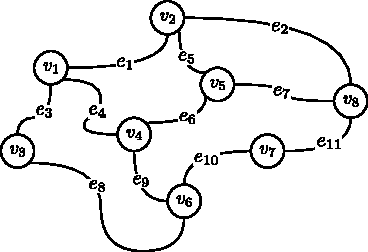
\includegraphics[width=\textwidth]{Chapter_I/DAG-UDAG-example/a}
		\caption{}
		\label{fig:dagudacExample:a}
	\end{subfigure}
	\hfill
	\begin{subfigure}[b]{0.32\textwidth}
		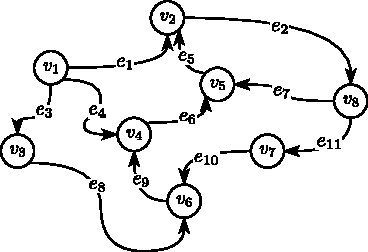
\includegraphics[width=\textwidth]{Chapter_I/DAG-UDAG-example/b}
		\caption{}
		\label{fig:dagudacExample:b}
	\end{subfigure}
	\hfill\null
	\caption{
		\textbf{(a)}~Nieskierowany graf $G = \left( V, E \right)$, gdzie $V = \left\{ v_{1}, v_{2}, \dots, v_{8} \right\}$ i $E = \left\{ e_{1}, e_{2}, \dots, e_{11} \right\}$.
		\textbf{(b)}~Skierowana wersja tego samego grafu.
	}
	\label{fig:dagudacExample}
\end{figure}

\subsection{Drzewo rozpinające}

Rozpoczniemy od definicji drzewa, które jest specyficznym rodzajem grafu:

\begin{definition}
	Drzewo jest spójnym grafem nie zawierającym żadnych cykli.
\end{definition}

\textbf{Grafem spójnym} z kolei nazywamy graf, którego wszystkie wierzchołki są ze sobą w dowolny sposób połączone --- do wszystkich z nich jesteśmy w stanie dojść z wykorzystaniem pewnej liczby krawędzi grafu. \textbf{Cyklem} zaś nazywamy taką ścieżkę w grafie, której wierzchołek początkowy jest jednocześnie węzłem na końcu tej ścieżki.

\begin{figure}[!htbp]
	\null\hfill
	\begin{subfigure}[b]{0.32\textwidth}
		\includegraphics[width=\textwidth]{Chapter_I/DEF-example/a}
		\caption{}
		\label{fig:defExample:a}
	\end{subfigure}
	\hfill
	\begin{subfigure}[b]{0.32\textwidth}
		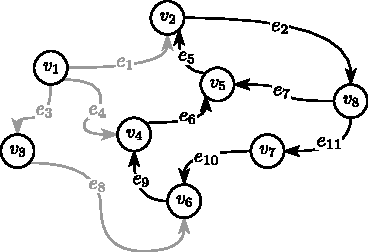
\includegraphics[width=\textwidth]{Chapter_I/DEF-example/b}
		\caption{}
		\label{fig:defExample:b}
	\end{subfigure}
	\hfill
	\begin{subfigure}[b]{0.32\textwidth}
		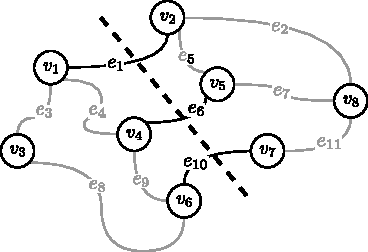
\includegraphics[width=\textwidth]{Chapter_I/DEF-example/c}
		\caption{}
		\label{fig:defExample:c}
	\end{subfigure}
	\hfill\null
	\caption{
		\textbf{(a)}~Graf nieskierowany $G^{\prime} = \left( V, E \right)$, gdzie $V = \left\{ v_{1}, v_{2}, \dots, v_{8} \right\}$ i $E = \left\{ e_{1}, e_{2}, \dots, e_{11} \right\}$ zawierający $5$ cykli: $\left\{ e_{1}, e_{2}, e_{7}, e_{6}, e_{9}, e_{8}, e_{3} \right\}$, $\left\{ e_{2}, e_{7}, e_{5} \right\}$, $\left\{ e_{2}, e_{7}, e_{6}, e_{4}, e_{1} \right\}$, $\left\{ e_{1}, e_{5}, e_{6} \right\}$, $\left\{ e_{1}, e_{5}, e_{6}, e_{9}, e_{8}, e_{3} \right\}$. Graf jest niespójny --- wierzchołek $v_{7}$ nie jest w żaden sposób połączony z pozostałymi wierzchołkami grafu.
		\textbf{(b)}~Graf skierowany posiadający tylko dwa cykle (zaznaczone czarnym kolorem): $\left\{ e_{2}, e_{7}, e_{5} \right\}$ oraz $\left\{ e_{2}, e_{11}, e_{10}, e_{9}, e_{6}, e_{5} \right\}$.
		\textbf{(c)}~Przykład cięcia w grafie.
	}
	\label{fig:defExample}
\end{figure}

\textbf{Drzewem rozpinającym} dany graf $G = \left( V, E \right)$ będziemy nazywać taki najmniej liczny zbiór krawędzi $T$, który łączy ze sobą wszystkie wierzchołki w grafie. Formanie:

\begin{equation}
	T = \left\{ e \in E : \left| T \right| = \left| V \right| - 1 \wedge \left( \forall v, v^{\prime} \in V : v \neq v^{\prime} \right) \; !\exists v \overset{\ast, T}{\leadsto} v^{\prime} \right\}\text{,}
\end{equation}
gdzie $\left| T \right|$ symbolizuje liczbę krawędzi w zbiorze $T$, $v \overset{\ast, E}{\leadsto} v^{\prime}$ wyraża dowolnej długości ścieżkę składającą się tylko z krawędzi generowanego zbioru $T$. Zbiór ten, jak widać z powyższej definicji, powinien mieć tę własność, że dla dowolnych dwóch różnych wierzchołków należących do grafu, istnieje dokładnie jedna ścieżka pomiędzy tymi wierzchołkami. Aby przekonać się, że liczba krawędzi należących do zbioru $T$ rzeczywiście powinna wynosić $\left| V \right| - 1$, możemy posłużyć się następującą konstrukcją:

\begin{itemize}
	\item poprowadźmy w grafie ścieżkę przechodzącą przez wszystkie wierzchołki dokładnie raz i kończącą się w wierzchołku początkowym (zbudujmy \textbf{cykl Hamiltona}) --- nie trudno zauważyć, że aby połączyć ze sobą wszystkie wierzchołki, potrzebujemy z każdego kolejnego wierzchołka poprowadzić nową krawędź. Otrzymujemy zatem cykl złożony z dokładnie $\left| V \right|$ krawędzi.
	\item Usuńmy teraz dowolną krawędź z cyklu. Ta operacja powoduje oczywiście jego przerwanie, zaś ze sposobu jego konstrukcji wynika, że pozostała ścieżka przechodzi kolejno przez wszystkie węzły w grafie --- tworzy drzewo rozpinające o liczbie krawędzi równej $\left| V \right| - 1$.
\end{itemize}

\section{Problem minimalnego drzewa rozpinającego}

Niech $\mathcal{T}_{G}$ oznacza zbiór wszystkich drzew rozpinających dla grafu $G$. Problem \textbf{minimalnego drzewa rozpinającego} polega na znalezieniu takiego zbioru krawędzi $T^{\ast} \in \mathcal{T}_{G}$, że ich całkowity koszt jest najmniejszy spośród wszystkich pozostałych możliwych rozwiązań. Zanim jednak bezpośrednio przejdziemy do omawiania algorytmów, które służą do odnajdywania konstrukcji o takich właściwościach, przedstawimy warunki jakie musi spełniać drzewo, abyśmy mieli pewność że suma kosztów jego krawędzi rzeczywiście jest najmniejsza.

Pierwszym takim podejściem do zdefiniowania warunków optymalności rozwiązania $T$ jest warunek \textbf{optymalnych cięć}. Zaprezentowany na rysunku \ref{fig:defExample:c} przykład prezentuje cięcie grafu $G$ --- w przypadku cięcia drzew rozpinających takie posunięcie spowoduje jego podział na dwie części, tak jak to pokazano na rysunkach \ref{fig:cut:a}--\ref{fig:cut:c}, gdyż w wyniku zastosowania cięcia przez wybraną krawędź jest ona usuwana z ciętego zbioru. Optymalnym cięciem natomiast będziemy nazywali takie cięcie, w wyniku którego z grafu usuwana jest krawędź o jak najmniejszym (w przypadku problemów minimalizacyjnych) koszcie ze wszystkich znajdujących się na drodze takiego cięcia (np. na rysunku \ref{fig:defExample:c} cięcie przechodzi przez krawędzie $\left\{ e_{1}, e_{6}, e_{10} \right\}$). W przypadku cięcia drzewa rozpinającego $T$ (patrz rysunek \ref{fig:cut}) przez krawędź $e_{6}$, zbiór taki będziemy oznaczać przez $\mathcal{Q} \left( T, e_{6} \right)$ i będą do niego należeć wszystkie krawędzie $e^{\prime} \in E$ łączące ze sobą dwa, powstałe w wyniku cięcia, zbiory wierzchołków, zgodnie z poniższą definicją.

\begin{equation}\label{eq:treecutedgeset}
\mathcal{Q} \left( T, e \right) = \left\{ \left( i, j \right) \; : \; v_{i} \in V_{1} \wedge v_{j} \in V_{2} \right\}
\end{equation}

\begin{theorem}[Kryterium optymalnych cięć (ang. \textit{Cut Optimality Conditions})]\label{def:optmstcut}
	Dla grafu $G = \left( V, E \right)$, drzewo rozpinające $T^{\ast}$ jest minimalnym drzewem rozpinającym dany graf wtedy i tylko wtedy, gdy dla każdej krawędzi $e_{ij} \in T^{\ast}$ jej koszt $c_{ij}$ jest najmniejszy spośród wszystkich krawędzi zbioru $\mathcal{Q} \left( T^{\ast}, e_{ij} \right)$, powstałego w wyniku cięcia drzewa $T^{\ast}$ przez krawędź $e_{ij}$.
\end{theorem}

Innymi słowy, przyglądając się rysunkowi \ref{fig:cut:b}, koszt krawędzi przez którą dokonujemy cięcia ($e_{6}$) musi być mniejszy bądź równy wagom krawędzi $e_{1}$ oraz $e_{10}$ --- własność ta powinna zachodzić dla każdego innego możliwego cięcia w drzewie rozpinającym (dla przykładu z omawianego rysunku tych cięć jest jeszcze $6$ --- każde takie cięcie usuwa z drzewa rozpinającego inną jego krawędź). W ogólnym przypadku liczba cięć równa się liczbie krawędzi należących do drzewa rozpinającego (jedno cięcie nie może przebiegać przez wiele krawędzi $e \in T$ naraz). Argument przemawiający za takim kryterium optymalności rozwiązania jest łatwy do zauważenia --- jeżeli krawędź $e_{6}$ (patrz \ref{fig:cut:b}) nie miałaby najmniejszego kosztu spośród wszystkich krawędzi należących do $\mathcal{Q} \left( T, e_{6} \right)$ (to jest albo $c_{1} < c_{6}$ albo $c_{10} < c_{6}$), wtedy usuwając z drzewa rozpinającego krawędź $e_{6}$ (zrywając połączenie między wierzchołkami grafu) a dodając do niego krawędź $e_{1}$ lub $e_{10}$ (zależnie od przypadku) stworzylibyśmy nowe drzewo rozpinające $T^{\prime}$ o koszcie oczywiście mniejszym niż koszt drzewa $T$. Zatem drzewo $T$ w takiej sytuacji z pewnością nie jest szukanym rozwiązaniem optymalnym.

\begin{proof}
	Dowód w pierwszą stronę, pokazujący że jeżeli drzewo $T$ jest minimalnym drzewem rozpinającym to musi spełniać podane kryterium, jest bardzo prosty, jego główną ideę zdążyliśmy już przedstawić, zatem skupimy się na pokazaniu odwrotnej zależności --- jeżeli drzewo $T^{\ast}$ spełnia warunki optymalnych cięć, musi być minimalnym drzewem rozpinającym. Załóżmy zatem, że drzewo $T$ jest minimalnym drzewem rozpinającym i jest różne od $T^{\ast}$. Z połączenia faktów, że $\left| T \right| = n - 1 = \left| T^{\ast} \right|$ i $T \neq T^{\ast}$ otrzymujemy wniosek, że do drzewa $T^{\ast}$ musi należeć choć jedna krawędź (niech będzie to łuk $e_{ij} \in T^{\ast}$), która nie należy do drugiego z drzew ($e_{ij} \notin T$). Usuńmy tą krawędź z $T^{\ast}$. Tym samym stworzymy podział drzewa $T^{\ast}$ na dwa poddrzewa --- $T_{1}$ oraz $T_{2}$ --- których wierzchołki łączone przez ich krawędzie podzielimy na zbiory $V_{1}$ i $V_{2}$. Spójrzmy teraz na drzewo $T$. Jego krawędzie oczywiście łączą ze sobą te same zbiory wierzchołków (składa się tylko z innych krawędzi). Z definicji zaś drzewa rozpinającego wiemy, że dodając do niego jeszcze jedną krawędź, stworzymy nim cykl. Dodajmy do niego zatem łuk, o którym wiemy, że nie należy do tego drzewa --- $e_{ij}$. Dodając do tego drzewa dodatkową krawędź stworzyliśmy cykl, którego elementy przynajmniej dwukrotnie przechodzą pomiędzy wierzchołkami należącymi do $V_{1}$ oraz $V_{2}$ (możemy tu odwołać się do rysunku \ref{fig:cut:b}, gdzie przedstawione na nim drzewo to $T^{\ast}$, zaś usuwana z niego krawędź $e_{ij}$ to łuk $e_{6}$ --- z założenia, że $e_{6} \notin T$ wiemy, że do $T$ musi należeć przynajmniej jeden z wierzchołków $\left\{ e_{1}, e_{10} \right\}$, tak aby zachować połączenie między wierzchołkami, więc dodanie do niego krawędzi $e_{6}$ owocuje obecnością dwóch takich wierzchołków, które łączą ze sobą węzły zbioru $V_{1}$ z tymi należącymi do $V_{2}$). Niech tą drugą krawędzią będzie krawędź $e_{kl}$. Drzewo $T^{ast}$ z założenia spełnia warunek optymalnych cięć tak więc $c_{ij} \leqslant c_{kl}$ (cięliśmy je wzdłuż krawędzi $c_{ij}$, więc z założenia wszystkie krawędzie należące do zbioru $\mathcal{Q} \left( T^{\ast}, e_{ij} \right)$ --- w tym $e_{kl}$ mają koszty nie mniejsze od wagi $e_{ij}$). Dodatkowo, na początku dowodu założyliśmy, że drzewo $T$ jest minimalnym drzewem rozpinającym graf (jest rozwiązaniem optymalnym) --- jego optymalność wymusza aby koszt krawędzi $e_{kl} \in T$ spełniał warunek $c_{kl} \leqslant c_{ij}$ (inaczej z pierwszej części dowodu natychmiast otrzymalibyśmy wynik, że $T$ nie jest optymalne). Z tych dwóch nierówności otrzymujemy, że $c_{ij} = c_{kl}$. Możemy zatem bezkarnie wymienić krawędź $e_{ij} \in T^{\ast}$ na łuk $e_{kl} \notin T^{\ast}$ --- otrzymane drzewo nadal będzie mieć takie same koszty (pozostanie rozwiązaniem optymalnym) a przy okazji liczba krawędzi różniących go od drzewa $T$ (optymalnego z założenia) ulegnie zmniejszeniu. Kontynuując powyższe czynności (wymieniając krawędzie drzewa $T^{\ast}$, które nie należą do $T$ na te, które są jego częścią), na pewnym etapie konstrukcji takiego drzewa okaże się, że skonstruowane drzewo jest drzewem zawierającym te same krawędzie co $T$ --- jako że po drodze ani razu nie zmienialiśmy kosztów konstruowanego drzewa możemy wyciągnąć wniosek, że drzewo $T^{\ast}$ (od którego wyszliśmy) od początku było optymalne, co mieliśmy udowodnić.
\end{proof}

\begin{figure}[!htbp]
	\null\hfill
	\begin{subfigure}[b]{0.32\textwidth}
		\includegraphics[width=\textwidth]{Chapter_I/CUT-example/a}
		\caption{}
		\label{fig:cut:a}
	\end{subfigure}
	\hfill
	\begin{subfigure}[b]{0.32\textwidth}
		\includegraphics[width=\textwidth]{Chapter_I/CUT-example/b}
		\caption{}
		\label{fig:cut:b}
	\end{subfigure}
	\hfill
	\begin{subfigure}[b]{0.32\textwidth}
		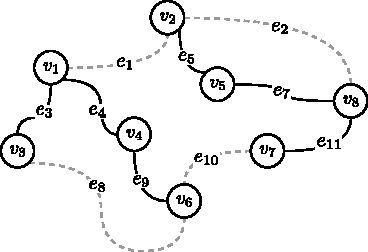
\includegraphics[width=\textwidth]{Chapter_I/CUT-example/c}
		\caption{}
		\label{fig:cut:c}
	\end{subfigure}
	\hfill\null
	\caption{
		\textbf{(a)}~Drzewo rozpinające dla grafu $G = \left( V, E \right)$, gdzie $V = \left\{ v_{1}, v_{2}, \dots, v_{8} \right\}$ i $E = \left\{ e_{1}, e_{2}, \dots, e_{11} \right\}$.
		\textbf{(b)}~Cięcie przez krawędź drzewa rozpinającego $e_{6}$ w grafie. Krawędzie leżące na cięciu zostały pogrubione.
		\textbf{(c)}~Zbiory wierzchołków $V_{1} = \left\{ v_{1}, v_{3}, v_{4}, v_{6} \right\}$ oraz $V_{2} = \left\{ v_{2}, v_{5}, v_{7}, v_{8} \right\}$ powstałe w wyniku podziału drzewa rozpinającego $T$ na mniejsze podddrzewa. Zbiór krawędzi $\mathcal{Q} \left( T, e_{6} \right)$ definiowany przez to cięcie zawiera elementy: $\left\{ e_{1}, e_{10} \right\}$.
	}
	\label{fig:cut}
\end{figure}

Alternatywnym warunkiem określającym optymalność rozwiązania problemu minimalnego drzewa rozpinającego jest kryterium optymalnych ścieżek (ang. \textit{Path Optimality Conditions}), które wygląda następująco:

\begin{theorem}{Kryterium optymalny ścieżek}\label{def:optpath}
	Drzewo rozpinające $T^{\ast}$ jest minimalnym drzewem rozpinającym wtedy i tylko wtedy, gdy dla każdej krawędzi spoza tego drzewa $e_{kl} \in E \setminus T^{\ast}$, dla każdej krawędzi $e_{ij} \in T^{\ast}$ należącej do ścieżki $v_{k} \overset{\ast}{\leadsto} v_{l}$ zachodzi $c_{ij} \leqslant c_{kl}$.
\end{theorem}

\begin{proof}
	Pokażmy, że jeśli drzewo $T^{\ast}$ jest minimalnym drzewem rozpinającym, to spełnia warunek optymalnych ścieżek.
	Dowód ten częściowo wynika z poprzedniego --- jeżeli drzewo $T^{\ast}$ jest optymalne i założymy, że istnieje taka krawędź $e_{ij}$ na ścieżce pomiędzy wierzchołkami $v_{k}$ a $v_{l}$ taka, że $c_{ij} > c_{kl}$, to dodając do drzewa krawędź $e_{ij}$ otrzymamy cykl, którego nie wszystkie koszty krawędzi są mniejsze od wagi nowo dodanego łuku. Aby na powrót otrzymać drzewo rozpinające musimy przerwać cykl, wyrzucając z rozwiązania jedną krawędź cyklu --- jako że własność optymalnej ścieżki nie była spełniona, wśród krawędzi cyklu na pewno jest łuk $e$, którego koszt jest większy od kosztu nowej krawędzi, zatem naturalnym posunięciem będzie usunąć właśnie ten łuk, by otrzymać jak najlepsze rozwiązanie. Usuwając go jednak otrzymujemy nowe rozwiązanie, którego koszt jest mniejszy od kosztu pierwotnego drzewa $T$, które było optymalne. Otrzymaliśmy zatem sprzeczność.
	Możemy także pokazać równoważność powyższych dwóch twierdzeń --- zauważmy, że jeśli dane drzewo $T^{\ast}$ podzielimy poprzez wykonanie cięcia wzdłuż krawędzi $e_{ij}$ (tak jak w poprzednim dowodzie tworząc zbiory $T_{1}$, $T_{2}$, $V_{1}$, $V_{2}$}), wybierzemy dowolną krawędź $e_{kl}$ taką, że $v_{k} \in V_{1}$ i $v_{l} \in V_{2}$, to z warunku optymalności ścieżki otrzymujemy natychmiast, że $c_{ij} \leqslant c_{kl}$, gdzie krawędź $e_{kl}$ jest dowolną krawędzią należącą do $\mathcal{Q} \left( T^{\ast}, e_{ij} \right)$ --- przedstawiona własność jest własnością optymalnego cięcia, którą drzewo $T^{\ast}$ spełnia zatem na mocy poprzedniego twierdzenia jest optymalne.
\end{proof}

\section{Znane algorytmy rozwiązujące problem MST}

Problem minimalnego drzewa rozpinającego jest bardzo dobrze znany toteż istnieje wiele algorytmów (ich wariacji)  radzących sobie z danym problemem. W tej części skupimy się na dwóch podstawowych: algorytmie Josepha Kruskala~\cite[$520$--$522$]{Ahuja:1993:NFT:137406}, Vojtěcha Jarníka (Prima)~\cite[$523$--$525$]{Ahuja:1993:NFT:137406}. Inne sposoby podejścia do problemu o jakich wspomnimy w następnych rozdziałach to: algorytm Chazelle'iego i również sobie z nim radzące modele programowania liniowego oraz całkowitoliczbowego (o tych ostatnich więcej opowiemy w rozdziale \ref{ch:linearprog}). Algorytmami, którymi się nie będziemy zajmować są natomiast: algorytm Tarjana oraz Borůvka.

\subsection{Algorytm Kruskala}

Pierwszym algorytmem, którego schemat działania omówimy, będzie algorytm Kruskala, który w bardzo dużym stopniu polega na udowodnionym przez nas kryterium optymalności drzewa rozpinającego --- optymalnych ścieżek (\ref{def:optpath}). Jak pamiętamy, zgodnie z podanym kryterium, drzewo rozpinające $T$ jest minimalnym drzewem rozpinającym grafu $G$ tylko wtedy, gdy wszystkie krawędzie nienależące do tego drzewa, zaś należące do ścieżki między dwoma wierzchołkami, które łączy krawędź należąca do $T$, mają koszt nie większy niż waga tej ostatniej. Definicja ta bezpośrednio przekłada się na ideę algorytmu: będziemy chcieli kolejno dodawać do naszego rozwiązania krawędzie w kolejności od ich najmniejszego kosztu do największej wagi, konstruując przy tym coraz to dłuższe ścieżki, aż do momentu, w którym na ścieżkach nie zaczną pojawiać się cykle. Dzięki uprzedniemu posortowaniu krawędzi względem ich kosztów mamy w tym przypadku pewność, że na takiej ścieżce znajdują się tylko krawędzie o najniższych kosztach, zaś wszystkie pozostałe łuki, które leżały na tej ścieżce (a których nie możemy już dodać ze względu na pojawienie się cyklu), mają większy koszt krawędzi niż ostatni łuk dodany do ścieżki. Naszym głównym celem zatem jest konstruowanie ścieżek --- w linii $8$ pseudokodu \ref{alg:kruskal} sprawdzamy, czy oba wierzchołki, które łączy analizowana przez nas krawędź nie należą do tego samego zbioru. Jeśli tak jest --- krawędź którą chcemy dodać utworzyłaby cykl na ścieżce, do której należą oba te wierzchołki, zatem nie chcemy dodawać takiej krawędzi. Oczywiście aby algorytm działał poprawnie, zakładamy że zbiór krawędzi, po którym iterujemy ($7$--$12$) jest odpowiednio posortowany. W przypadku chęci dodania kolejnej krawędzi do ścieżki (gdy krawędź łączy różne zbiory --- $T_{0} \neq T_{1}$) musimy zaś połączyć ze sobą zbiory $T_{0}$ i $T_{1}$. Całość prezentuje się w formie pseudokodu zamieszczonego w \ref{alg:kruskal}.

\begin{pseudokod}[!htbp]
	\DontPrintSemicolon
	\SetKwInOut{Input}{Wejście}  
	\Input{
		$G = \left( V, E \right)$ --- graf wejściowy,\\
	}
	\SetKwInOut{Result}{Wyjście}  
	\Result{$T^{\ast}$ --- minimalne drzewo rozpinające.}
	\Begin{
		$T^{\ast} \leftarrow \emptyset$\;
		$\mathcal{T} \leftarrow \emptyset$\;
		\ForEach{$v \in V$}{
			$\mathcal{T} \leftarrow \mathcal{T} \cup \left\{ v \right\}$\;
		}
		$\textsc{inc-order} \left( E \right)$\;
		\ForEach{$e_{ij} \in E$}{
			\If{$\left( T_{0} : v_{i} \in T_{0} \right) \neq \left( T_{1} : v_{i} \in T_{1} \right)$}{
				$T^{\ast} \leftarrow T^{\ast} \cup e_{ij}$\;
				$\mathcal{T} \leftarrow \mathcal{T} \setminus T_{0}$\;	
				$\mathcal{T} \leftarrow \mathcal{T} \setminus T_{1}$\;	
				$\mathcal{T} \leftarrow \mathcal{T} \cup \left\{ v : v \in T_{0} \cup T_{1} \right\}$\;	
			}	
		}
		\Return $T^{\ast}$\;
	}
	\caption{\textsc{kruskal-mst} $\left( G \right)$}
	\label{alg:kruskal}
\end{pseudokod}

Czas działania takiego algorytmu oczywiście zależy od sposobu zaimplementowania linii $5$ oraz $8$--$12$, lecz górna jego granica to $O \left( m + n \cdot \log \left( n \right) \right)$~\cite[$522$]{Ahuja:1993:NFT:137406}.

\begin{figure}[!htbp]
	\null\hfill
	\begin{subfigure}[b]{0.24\textwidth}
		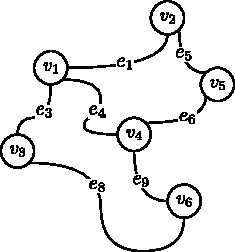
\includegraphics[width=\textwidth]{Chapter_I/KRUSKAL-example/a}
		\caption{}
		\label{fig:kruskal:a}
	\end{subfigure}
	\hfill
	\begin{subfigure}[b]{0.24\textwidth}
		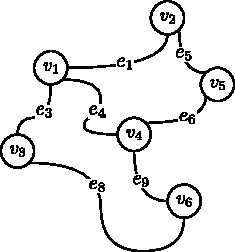
\includegraphics[width=\textwidth]{Chapter_I/KRUSKAL-example/a}
		\caption{}
		\label{fig:kruskal:b}
	\end{subfigure}
	\hfill
	\begin{subfigure}[b]{0.24\textwidth}
		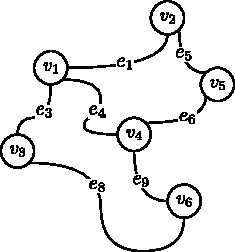
\includegraphics[width=\textwidth]{Chapter_I/KRUSKAL-example/a}
		\caption{}
		\label{fig:kruskal:c}
	\end{subfigure}
	\hfill
	\begin{subfigure}[b]{0.24\textwidth}
		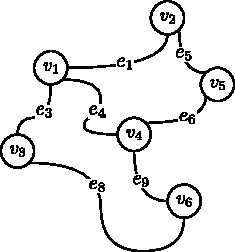
\includegraphics[width=\textwidth]{Chapter_I/KRUSKAL-example/a}
		\caption{}
		\label{fig:kruskal:d}
	\end{subfigure}
	\hfill\null
	\null\hfill
	\begin{subfigure}[b]{0.24\textwidth}
		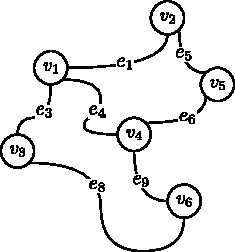
\includegraphics[width=\textwidth]{Chapter_I/KRUSKAL-example/a}
		\caption{}
		\label{fig:kruskal:e}
	\end{subfigure}
	\hfill
	\begin{subfigure}[b]{0.24\textwidth}
		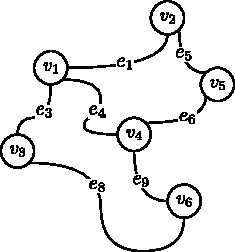
\includegraphics[width=\textwidth]{Chapter_I/KRUSKAL-example/a}
		\caption{}
		\label{fig:kruskal:f}
	\end{subfigure}
	\hfill
	\begin{subfigure}[b]{0.24\textwidth}
		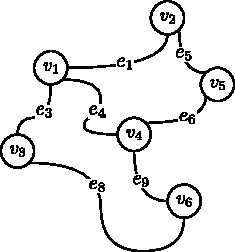
\includegraphics[width=\textwidth]{Chapter_I/KRUSKAL-example/a}
		\caption{}
		\label{fig:kruskal:g}
	\end{subfigure}
	\hfill
	\begin{subfigure}[b]{0.24\textwidth}
		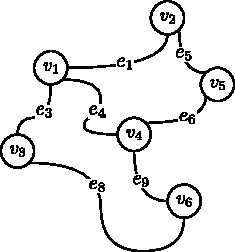
\includegraphics[width=\textwidth]{Chapter_I/KRUSKAL-example/a}
		\caption{}
		\label{fig:kruskal:h}
	\end{subfigure}
	\hfill\null
	\caption{
		\textbf{(a)}~Drzewo rozpinające dla grafu $G = \left( V, E \right)$, gdzie $V = \left\{ v_{1}, v_{2}, \dots, v_{8} \right\}$ i $E = \left\{ e_{1}, e_{2}, \dots, e_{11} \right\}$.
		\textbf{(b)}~Cięcie przez krawędź drzewa rozpinającego $e_{6}$ w grafie. Krawędzie leżące na cięciu zostały pogrubione.
		\textbf{(c)}~Zbiory wierzchołków $V_{1} = \left\{ v_{1}, v_{3}, v_{4}, v_{6} \right\}$ oraz $V_{2} = \left\{ v_{2}, v_{5}, v_{7}, v_{8} \right\}$ powstałe w wyniku podziału drzewa rozpinającego $T$ na mniejsze podddrzewa. Zbiór krawędzi $\mathcal{Q} \left( T, e_{6} \right)$ definiowany przez to cięcie zawiera elementy: $\left\{ e_{1}, e_{10} \right\}$.
	}
	\label{fig:cut}
\end{figure}

\subsection{Algorytm Prima}

\begin{pseudokod}[!htbp]
	\DontPrintSemicolon
	\SetKwInOut{Input}{Wejście}  
	\Input{
		$G = \left( V, E \right)$ --- graf wejściowy,\\
		$v_{1}$ --- węzeł początkowy, od którego rozpocznie się konstrukcja rozwiązania.
	}
	\SetKwInOut{Result}{Wyjście}  
	\Result{$T^{\ast}$ --- minimalne drzewo rozpinające.}
	\Begin{
		\ForEach{$v \in V \setminus \left( v_{1} \cup \left\{ v^{\prime} : v_{1} \leadsto v^{\prime} \right\} \right)$}{
			$v.d \leftarrow \infty$\;
		}
		$v_{1}.d \leftarrow 0$\;
		\ForEach{$v_{i} : v_{1} \leadsto v_{i}$}{
			$v_{i}.d \leftarrow c_{1i}$\;
			$v_{i}.p \leftarrow v_{1}$\;
		}
		$H \leftarrow \textsc{create-heap} \left( G \right)$\;
		\ForEach{$v \in V$}{
			$\textsc{insert} \left( v, H \right)$\;
		}
		$T^{\ast} \leftarrow \emptyset$\;
		\While{$\left| T^{\ast} \right| < \left| V \right| - 1$}{
			$v_{i} \leftarrow \textsc{find-min} \left( H \right)$\;
			$\textsc{delete-min} \left( H \right)$\;
			$T^{\ast} \leftarrow T^{\ast} \cup \left( v_{i}.p \leadsto v_{i} \right)$\;
			\ForEach{$ j : v_{i} \leadsto v_{j} \wedge v_{j} \in H$}{
				\If{$v_{j}.d > c_{ij}$}{
					$v_{j}.c \leftarrow c_{ij}$\;
					$v_{j}.p \leftarrow v_{i}$\;
					$\textsc{dec-key} \left( j, c_{ij}, H \right)$\;	
				}	
			}
		}
		\Return $T^{\ast}$\;
	}
	\caption{\textsc{prime-mst} $\left( G, v_{1} \right)$}
	\label{alg:prime}
\end{pseudokod}

\section{Podsumowanie rozdziału}

Problem minimalnego drzewa rozpinającego jest jednym z fundamentalnych problemów optymalizacyjnych pojawiających się w wielu dziedzinach codziennego życia. Wszędzie tam, gdzie może nam zależeć na np. jak największym uproszczeniu badanej struktury grafowej, pozbycia się redundantnych rozwiązań, bardzo prawdopodobnym jest, że napotkamy właśnie problem minimalnego drzewa rozpinającego. Uogólniając, zależnie od sposobu interpretacji elementów grafu możemy znaleźć wiele zastosowań dla wspomnianego problemu. Warto też zauważyć, że nie musimy ograniczać się tylko do problemu znalezienia rozwiązania o najmniejszej sumie kosztów --- jeżeli nasze koszty będą skonstruowane w ten sposób, że każdy z nich przybierać będzie postać logarytmu o ustalonej podstawie, ich suma tak naprawdę będzie wyrażać iloczyn rzeczywistych kosztów jakie chcieliśmy w problemie zawrzeć. Tworzy nam to jeszcze więcej możliwości zastosowania tak postawionego problemu~\cite[$512$--$516$]{Ahuja:1993:NFT:137406}.

Zapoznawszy się z podstawowymi pojęciami dotyczącymi problemów grafowych, naszą uwagę w następnych rozdziałach poświęcimy problemom bardziej złożonym, u podstaw których znajdziemy właśnie problem minimalnego drzewa rozpinającego (widzimy zatem, że jego zastosowania nie kończą się tylko na bezpośrednim zidentyfikowaniu problemu jako minimalnego drzewa rozpinającego, lecz jest on również podstawą do rozwiązywania wielu innych, bardziej złożonych problemów). W tym zaś przedstawiliśmy podstawowe narzędzia pozwalające nam na uporanie się z nim, przedstawiliśmy warunki optymalności takiej konstrukcji oraz przytoczyliśmy liczne definicje, z których będziemy korzystać we wszystkich następnych rozdziałach.
	\clearpage
	
	\clearpage
	\chapter{Odporna optymalizacja}\label{ch:minmax}
\thispagestyle{chapterBeginStyle}





W poprzednim rozdziale zapoznaliśmy się z~podstawowymi informacjami na temat problemu odnajdywania minimalnych drzew rozpinających w~grafach oraz poznaliśmy sposoby radzenia sobie z~nim.
Do tej pory jednak nie poruszyliśmy najistotniejszego dla nas tematu: \textbf{optymalizacji odpornej} na czynniki zewnętrzne.
Co przez to należy rozumieć?
Do tej pory poznaliśmy algorytmy, które potrafią rozwiązywać problem w~środowisku zamkniętym~--- idealnym, w~którym nic nie ma prawa się zmieniać przez cały czas pracy algorytmu.
W~tym rozdziale omówimy modele problemów nie posiadających takiego ograniczenia~--- w~modelach tych dane nie tylko będą mogły się zmieniać, ale będziemy także dopuszczać możliwość bycia nieświadomym tych zmian.
W~charakterze podsumowania, formalnie zapiszemy model jednego z~wariantów przedstawionych problemów, wskazując tym samym ogólne podejście do jego rozwiązania.




\section{Scenariusze dyskretne a~ciągłe}




W poprzednim rozdziale skupialiśmy swoją uwagę na problemie wyszukiwania minimalnego drzewa rozpinającego w~grafie $G = \left( V, E \right)$, czyli takiego zbioru krawędzi $T^{\ast}$, który łączył ze sobą wszystkie wierzchołki w~grafie, a~jednocześnie którego suma kosztów krawędzi $e \in T^{\ast}$ była możliwie najmniejsza.
Formalnie:

\begin{equation}
	T^{\ast}_{G = \left( V, E \right)} = \left\{ e \in E \; : \; T^{\ast}_{G = \left( V, E \right)} \in \mathcal{T}_{G} \; \wedge \; \left( \forall T^{\prime} \in \mathcal{T}_{G} \right) \; \sum_{ \mathclap{e \in T^{\prime} }} c_{e} \geqslant c_{ T^{\ast}_{ G = \left( V, E \right) } } \right\}\text{,}
\end{equation}
gdzie $\mathcal{T}_{G}$ oznaczał zbiór wszystkich drzew możliwych do skonstruowania w~grafie $G$, $c_{e}$~--- koszt krawędzi $e \in E$, zaś $\sum_{ e \in T^{\prime} } c_{e} = c_{T^{\prime}}$~--- sumę kosztów wszystkich krawędzi, która wynika ze \textbf{scenariusza}.
Scenariuszem $\textbf{s}$ zatem nazwiemy zbiór definiujący koszt dla każdej krawędzi w~grafie: $\textbf{s} = \left\{ c^{\textbf{s}}_{e_{i}} : i \in \left\{ 1, \dots, \left| E \right| \right\} \right\}$.
Na rysunku \ref{fig:scenarioExample} odpowiednio widzimy przykłady trzech różnych scenariuszy, zastosowanych do tego samego drzewa.
Rzecz jasna, zależnie od kosztów jakie zostaną narzucone krawędziom przez dany scenariusz, zwracane przez dotychczas poznane algorytmy rozwiązania będą się różnić.
Zwróćmy uwagę na rysunek \ref{fig:scenarioExample:b}, gdzie celowo nie zostały ujawnione koszty scenariusza~--- jedyne co o~nim wiemy to to, że żaden koszt krawędzi w~tym scenariuszu nie jest mniejszy od kosztu odpowiadającej mu krawędzi w~$\textbf{s}_{1}$, ani większy od kosztu tej samej krawędzi w~scenariuszu $\textbf{s}_{3}$.
Taki rodzaj scenariusza nazywamy \textbf{scenariuszem ciągłym}, zaś scenariusze, których poszczególne koszty krawędzi są najmniejsze (bądź największe) spośród wszystkich scenariuszy, nazywamy \textbf{scenariuszami granicznymi/krytycznymi} (odpowiednio \textbf{scenariuszem najlepszego/najgorszego przypadku}).

\begin{figure}[!htbp]
	\null\hfill
	\begin{subfigure}[b]{0.32\textwidth}
		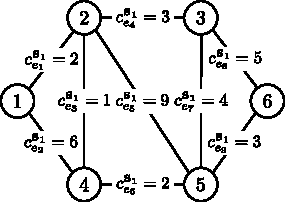
\includegraphics[width=\textwidth]{Chapter_II/SCENARIO-example/a}
		\caption{}
		\label{fig:scenarioExample:a}
	\end{subfigure}
	\hfill
	\begin{subfigure}[b]{0.32\textwidth}
		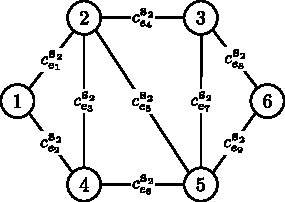
\includegraphics[width=\textwidth]{Chapter_II/SCENARIO-example/b}
		\caption{}
		\label{fig:scenarioExample:b}
	\end{subfigure}
	\hfill
	\begin{subfigure}[b]{0.32\textwidth}
		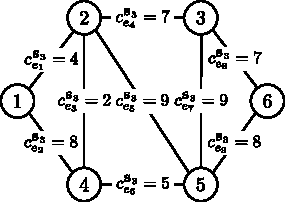
\includegraphics[width=\textwidth]{Chapter_II/SCENARIO-example/c}
		\caption{}
		\label{fig:scenarioExample:c}
	\end{subfigure}
	\hfill\null
	\caption{
		Scenariusze $\textbf{s}_{1}$, $\textbf{s}_{2}$, $\textbf{s}_{3}$ dla grafu nieskierowanego $G = \left( V, E \right)$, $V = \left\{ 1, 2, \dots, 6 \right\}$, $E = \left\{ e_{i} : i \in \left\{ 1, \dots, 9 \right\} \right\}$.
		\textbf{(a)}~Scenariusz najlepszego przypadku $\textbf{s}_{1} = \left[ 2, 6, 1, 3, 9, 2, 4, 5, 3 \right]$.
		Dla scenariusza zachodzi: $\left( \forall i \in \left\{ 1, \dots, 9 \right\} \right) c^{\textbf{s}_{1}}_{e_{i}} \leqslant c^{\textbf{s}_{2}}_{e_{i}}$.
		Scenariusz o~takich właściwościach będziemy też oznaczać jako $\underline{\textbf{s}}$.
		\textbf{(b)}~Scenariusz ciągły $\textbf{s}_{2}$.
		Koszty tego scenariusza zdefiniowane są następująco: $\left( \forall i \in \left\{ 1, \dots, 9 \right\} \right) c^{\underline{\textbf{s}}}_{e_{i}} \leqslant c^{\textbf{s}_{2}}_{e_{i}} \leqslant c^{\overline{\textbf{s}}}_{e_{i}}$.
		\textbf{(c)}~Krytyczny scenariusz najgorszego przypadku $\textbf{s}_{3} = \left[ 4, 8, 2, 7, 9, 5, 9, 7, 8 \right]$.
		Dla scenariusza zachodzi: $\left( \forall i \in \left\{ 1, \dots, 9 \right\} \right) c^{\textbf{s}_{2}}_{e_{i}} \leqslant c^{\textbf{s}_{3}}_{e_{i}}$.
		Scenariusz o~takich właściwościach będziemy też oznaczać jako $\overline{\textbf{s}}$.
	}
	\label{fig:scenarioExample}
\end{figure}

Przedstawione rodzaje scenariuszy można rozważać dla wszystkich problemów odpornej optymalizacji dyskretnej jakie tutaj wymienimy.
W~przypadku problemu minimalizacyjnego, jakim jest omawiany przez nas problem znajdowania minimalnego drzewa rozpinającego, krytyczne scenariusze najlepszego i~najgorszego przypadku będziemy oznaczać odpowiednio przez $\underline{\textbf{s}}$ oraz $\overline{\textbf{s}}$, gdzie $0 \leqslant \underline{\textbf{s}} \leqslant \overline{\textbf{s}}$.
Dla problemów maksymalizacyjnych znaczenie przedstawionych symboli byłoby zgoła odwrotne: $\overline{\textbf{s}}$ oznaczałby krytyczny scenariusz o~największych współczynnikach (najlepszego przypadku), zaś $\underline{\textbf{s}}$~--- najgorszego, gdzie każdy jego współczynnik nie byłby większy od dowolnego z~odpowiadających mu współczynników w~pozostałych scenariuszach.
\textbf{Scenariuszem dyskretnym} (ang. \textit{discrete scenario}) będziemy natomiast nazywać każdy scenariusz, który ma zdefiniowane koszty dla każdej krawędzi.
Takimi scenariuszami są na przykład scenariusze krytyczne (ang. \textit{extreme scenarios}).




\section{Problemy minimaksowe}




Problemami minimaksowymi~\cite[$428$]{minmaxSurvey} nazywamy problemy, których celem jest odnalezienie najlepszego rozwiązania przy założeniu wystąpienia najgorszych z~możliwych scenariuszy dla danych rozwiązań.
Możemy rozróżnić tutaj problemy typu \textsc{Min-Max} (\ref{eq:minmax}) oraz \textsc{Max-Min} (\ref{eq:maxmin}):

\noindent\begin{minipage}{.3\linewidth}
	\begin{equation}\label{eq:minmax}
		\min_{ \mathclap{\textbf{x} \in X}} \max_{ \mathclap{\textbf{s} \in \mathcal{S}}} v \left( \textbf{x}, \textbf{s} \right)
	\end{equation}
\end{minipage}%
\begin{minipage}{.3\linewidth}
	\centering
	oraz
\end{minipage}%
\begin{minipage}{.3\linewidth}
	\begin{equation}\label{eq:maxmin}
	\max_{ \mathclap{\textbf{x} \in X}} \min_{ \mathclap{\textbf{s} \in \mathcal{S}}} v \left( \textbf{x}, \textbf{s} \right) \text{,}
	\end{equation}
\end{minipage}
\vspace{5px}
\\
przy czym $\textbf{x}$ jest rozwiązaniem problemu, wybranym ze zbioru wszystkich możliwych rozwiązań $X$, $v \left( \textbf{x}, \textbf{s} \right)$ reprezentuje koszt rozwiązania problemu dla scenariusza $\textbf{s}$ i~wybranego zbioru krawędzi $\left\{ e \in E : x_{e} = 1 \right\}$\footnote{
	Często dla własnej wygody będziemy zamiennie stosować oznaczenia: $x_{e}$ oraz $x_{e_{i}}$ (lub $x_{i}$) dla zmiennej decyzyjnej w~wektorze $\textbf{x}$, będącym wybranym rozwiązaniem problemu minimalnego drzewa rozpinającego, czy też $c_{e}$ i~$c_{e_{i}}$ (lub $c_{i}$) dla oznaczeń kosztów krawędzi, chyba że zostanie napisane inaczej.
	Oznaczenia $x_{e_{i}}$/$x_{i}$ oraz $c_{e_{i}}$/$c_{i}$ będziemy stosować w~przypadku, gdy będzie wymagane zachowanie kolejności oznaczeń np. dla krawędzi występujących w~zbiorze kolejno po sobie ($x_{e_{i}}$, $x_{e_{i+1}}$, $\dots$).
}, zaś $S$ reprezentuje zbiór dostępnych scenariuszy.
Oczywiście w~przypadku gdy $\left| S \right| = 1$, problem \textsc{Min-Max Spanning Tree} sprowadza się do klasycznego problemu minimalnego drzewa rozpinającego.



\subsection{Przypadek ciągły}



Niech $S = \left\{ \textbf{s} : \left( \forall i \in \left\{ 1, \dots, \left| E \right| \right\} \right) \; c^{\textbf{s}}_{e} \in \left[ c^{\underline{\textbf{s}}}_{e}, c^{\overline{\textbf{s}}}_{e} \right] \right\}$, gdzie scenariusze $\underline{\textbf{s}}$ i~$\overline{\textbf{s}}$ są odpowiednio scenariuszami przedstawionymi na rysunkach \ref{fig:scenarioExample:a} i~\ref{fig:scenarioExample:c}, zaś $c^{\textbf{s}}_{e}$ oznacza koszt krawędzi $e$ dla scenariusza $\textbf{s}$.
Innymi słowy: zbiór scenariuszy $S$ składa się z~takich schematów kosztów $\textbf{s}$, że każdy koszt krawędzi $c^{\textbf{s}}_{e}$ w~tym scenariuszu może przyjmować wartość należącą do przedziału $\left[ c^{\underline{\textbf{s}}}_{e}, c^{\overline{\textbf{s}}}_{e} \right]$.
Naszym celem niech będzie rozwiązanie problemu \textsc{Interval Min-Max Spanning Tree}.

Jak łatwo zauważyć, w~przypadku ciągłym zachodzi następująca prawidłowość:

\begin{equation}
		\min_{ \mathclap{\textbf{x} \in X}} \left( \max_{ \mathclap{\textbf{s} \in \mathcal{S}}} v \left( \textbf{x}, \textbf{s} \right) \right) = \min_{ \mathclap{\textbf{x} \in X}} \left( \max_{ \mathclap{\textbf{s} \in \mathcal{S}}} \sum_{e \in E} x_{e} \cdot c^{\textbf{s}}_{e} \right) = \min_{ \mathclap{\textbf{x} \in X}} \left( \sum_{ \mathclap{e \in E}} x_{e} \cdot c^{\overline{\textbf{s}}}_{e} \right) = \min_{ \mathclap{\textbf{x} \in X}} v \left( \textbf{x}, \overline{\textbf{s}} \right) \text{,}
\end{equation}
jako że dla scenariusza $\overline{\textbf{s}}$ i~każdego definiowanego przez niego kosztu, dla dowolnego scenariusza $\textbf{s} \in S$ zachodzi: $c^{\overline{\textbf{s}}}_{e} \geqslant c^{\textbf{s}}_{e}$.
Podobne rozumowanie możemy przeprowadzić dla problemu \textsc{Max-Min}.
Widzimy zatem, że w~przypadku tak postawionego problemu, dla scenariuszy o~rozmytych/niepewnych kosztach bardzo łatwo możemy znaleźć jego rozwiązanie, redukując problem do klasycznego problemu z~jednym, krytycznym scenariuszem.



\subsection{Przypadek dyskretny}



Powróćmy raz jeszcze do rysunku \ref{fig:scenarioExample}.
Niech tym razem naszym zbiorem scenariuszy będzie $S = \left\{ \textbf{s}_{1}, \textbf{s}_{3} \right\}$, gdzie $\textbf{s}_{1}$ i~$\textbf{s}_{3}$ odnoszą się odpowiednio do \ref{fig:scenarioExample:a} oraz \ref{fig:scenarioExample:c}.
\textbf{Dyskretnym} zbiorem scenariuszy nazwiemy taki zbiór, którego elementy jesteśmy w~stanie ponumerować (będący zbiorem przeliczalnym)~--- tutaj nasz zbiór scenariuszy posiada dokładnie dwa elementy.

\begin{figure}[!htbp]
	\null\hfill
	\begin{subfigure}[b]{0.35\textwidth}
		\includegraphics[width=\textwidth]{Chapter_II/MIN-MAX-DESC-example/a}
		\caption{}
		\label{fig:minmaxdesc:a}
	\end{subfigure}
	\hfill
	\begin{subfigure}[b]{0.35\textwidth}
		\includegraphics[width=\textwidth]{Chapter_II/MIN-MAX-DESC-example/b}
		\caption{}
		\label{fig:minmaxdesc:b}
	\end{subfigure}
	\hfill\null
	\caption{
		Dyskretne scenariusze $\textbf{s}_{1}$, $\textbf{s}_{3}$ dla grafu nieskierowanego $G = \left( V, E \right)$, $V = \left\{ 1, 2, \dots, 6 \right\}$, $E = \left\{ e_{i} : i \in \left\{ 1, \dots, 9 \right\} \right\}$, z~zaznaczonymi minimalnymi drzewami rozpinającymi dla każdego z~nich.
	}
	\label{fig:minmaxdesc}
\end{figure}

Pomimo tak prosto zdefiniowanego zadania przekonamy się, że jego rozwiązanie wcale nie jest tak intuicyjne jak oczekujemy~--- w~tabeli \ref{tab:minmaxexample} przedstawiono kilka z~$55$ możliwych rozwiązań zadanego problemu\footnote{
	Rozważane przykłady grafów posiadają $9$ krawędzi łączących jego wierzchołki~--- spośród wszystkich możliwych $512$ kombinacji zbiorów krawędzi, należących do rozwiązania (każda z~nich może do niego niezależnie należeć bądź nie, co daje nam $2^{9}$ możliwości wyboru rozwiązania), tylko $55$ z~nich zawiera krawędzie, które tworzą drzewo rozpinające dla danego grafu.
	Rozwiązania zostały wygenerowane poprzez modyfikację wszystkich kosztów w~grafie (ustawieniu ich na $0$) i~pobranie wszystkich optymalnych rozwiązań dla tak zadanego problemu (w takim przypadku każde dopuszczalne rozwiązanie było także rozwiązaniem optymalnym~--- więcej o~zagadnieniu optymalności opowiemy w~rozdziale \ref{ch:linearprog}, poświęconym programowaniu liniowemu).}.
Na uwagę w~niej zasługują rozwiązania $\textbf{x}_{1}$ oraz $\textbf{x}_{2}$, które są rozwiązaniami optymalnymi dla scenariuszy $\textbf{s}_{3}$ i~$\textbf{s}_{1}$, rozpatrywanych osobno.
Jeżeli spojrzymy na ostatnią kolumnę, zauważymy, że optymalne rozwiązanie dla pierwszego z~wymienionych scenariuszy jest także rozwiązaniem optymalnym problemu minimaksowego~--- tak jak w~przypadku scenariuszy ciągłych, tak i~tutaj mogliśmy skorzystać z~posiadanej wiedzy o~kosztach definiowanych przez każdy ze scenariuszy; wiedząc, że dla scenariusza $\textbf{s}_{3}$ żaden koszt nie jest mniejszy od odpowiadającej mu wagi w~drugim scenariuszu, nie powinno być dla nas zaskoczeniem, że optymalność rozwiązania problemu dla scenariusza o~wyższych kosztach pociąga za sobą optymalność rozwiązania problemu \textsc{Min-Max}.
Należy jednak podkreślić, że taka sytuacja jest zazwyczaj mało prawdopodobna i~bardzo łatwo możemy stworzyć scenariusze, dla których ta prawidłowość nie będzie zachodziła.

\begin{table}[!htbp]
	\caption{
		Tabela przedstawiająca część z~dopuszczalnych (ang. \textit{feasible}) rozwiązań dla problemu minimalnego drzewa rozpinającego dla scenariuszy $\textbf{s}_{1}$ oraz $\textbf{s}_{3}$ (\ref{fig:minmaxdesc:a} i~\ref{fig:minmaxdesc:b}), koszty dla każdego z~proponowanych rozwiązań dla podanych scenariuszy oraz wartość rozwiązania dla problemu minimaksowego.
		Wiersze w~tabeli zostały posortowane w~kolejności rosnących wartości rozwiązań.}
	\label{tab:minmaxexample}
	\begin{tabular}{ccccccccccccc}
		\cline{11-13}
		\multicolumn{2}{l}{}       &         &         &         &         &         &         &         &         & \multicolumn{3}{c}{Scenariusze}                                                                                                                                                                                              \\
		$X$              & $e_{1}$ & $e_{2}$ & $e_{3}$ & $e_{4}$ & $e_{5}$ & $e_{6}$ & $e_{7}$ & $e_{8}$ & $e_{9}$ & $v \left( \textbf{x}, \textbf{s}_{1} \right) $ & $ v \left( \textbf{x}, \textbf{s}_{3} \right) $ & $\max \left\{ v \left( \textbf{x}, \textbf{s}_{1} \right), v \left( \textbf{x}, \textbf{s}_{3} \right) \right\} $ \\
		$\textbf{x}_{1}$ & $1$     & $0$     & $1$     & $1$     & $0$     & $1$     & $0$     & $1$	&	$0$	&	$13$	&	$25$	&	$25$	\\
		$\textbf{x}_{2}$ & $1$     & $0$     & $1$     & $1$     & $0$     & $1$     & $0$     & $0$	&	$1$	&	$11$	&	$26$	&	$26$	\\
		$\textbf{x}_{3}$ & $1$     & $0$     & $1$     & $0$     & $0$     & $1$     & $0$     & $1$	&	$1$	&	$13$	&	$26$	&	$26$	\\
		$\textbf{x}_{4}$ & $1$     & $0$     & $1$     & $0$     & $0$     & $1$     & $1$     & $1$	&	$0$	&	$14$	&	$27$	&	$27$	\\
		$\dots$ & $\dots$     & $\dots$     & $\dots$     & $\dots$     & $\dots$     & $\dots$     & $\dots$     & $\dots$	&	$\dots$	&	$\dots$	&	$\dots$	&	$\dots$	\\
		$\textbf{x}_{53}$ & $1$     & $1$     & $0$     & $0$     & $1$     & $0$     & $1$     & $0$	&	$1$	&	$24$	&	$38$	&	$38$	\\
		$\textbf{x}_{54}$ & $0$     & $1$     & $0$     & $0$     & $1$     & $1$     & $1$     & $1$	&	$0$	&	$26$	&	$38$	&	$38$	\\
		$\textbf{x}_{55}$ & $0$     & $1$     & $0$     & $0$     & $1$     & $1$     & $1$     & $0$	&	$1$	&	$24$	&	$39$	&	$39$	\\
		 \hline
	\end{tabular}
\end{table}

Niech scenariusze $\textbf{s}_{4}$ i~$\textbf{s}_{5}$ będą takie, że dla każdego $e_{i}$, $i \in \left\{ 1, \dots, \left| E \right| - 2 \right\}$, $c^{\textbf{s}_{4}}_{e} = c^{\textbf{s}_{5}}_{e}$ oraz niech $c^{\textbf{s}_{4}}_{e_{\left| E \right| - 1}} = c^{\textbf{s}_{5}}_{e_{\left| E \right| - 1}} + 1$ i~$c^{\textbf{s}_{4}}_{e_{\left| E \right|}} = c^{\textbf{s}_{5}}_{e_{\left| E \right|}} - 1$, tak jak to pokazano na rysunku \ref{fig:minmaxexample}.
Usiłując rozwiązać postawiony przed nami problem postaci: $\min_{\textbf{x} \in X} \max_{\textbf{s} \in \mathcal{S}} v \left( \textbf{x}, \textbf{s} \right)$, szybko zauważymy, że w~tym przypadku odnalezienie optymalnych rozwiązań dla każdego ze scenariuszy i~próba wybrania spośród nich jednego, jako rozwiązania problemu \textsc{Min-Max Spanning Tree}, nie jest dobrym pomysłem: dla scenariusza $\textbf{s}_{4}$ optymalnym wyborem jest każdy podzbiór zbioru krawędzi grafu tworzący drzewo rozpinające, który nie zawiera łuku $e_{8}$ o~koszcie $a+1$ (koszt takiego rozwiązania wynosi $a \cdot \left( \left| V \right| - 1 \right)$), dla scenariusza $\textbf{s}_{5}$ uzyskamy podobne wyniki, tym razem wykluczając ze zbioru rozwiązań te podzbiory, do których należy krawędź $e_{9}$.
W~obu przypadkach wartość optymalnego rozwiązania wynosi tyle samo, zaś prawidłowym rozwiązaniem problemu $\min_{\textbf{x} \in X} \max_{\textbf{s} \in \mathcal{S}} v \left( \textbf{x}, \textbf{s} \right)$ jest rozwiązanie dowolne~--- analizowany graf i~jego koszty zostały tak dobrane, że wartość wyrażenia $\max_{\textbf{s} \in \mathcal{S}} v \left( \textbf{x}, \textbf{s} \right) = 5 \cdot a + 1$ dla każdego dopuszczalnego rozwiązania.
Wystarczy zauważyć, że jedyną istotną decyzją jaką musimy podjąć, jest wybór ostatniej krawędzi, zaś~--- niezależnie od dokonanego wyboru~--- maksymalny koszt wszystkich wybranych krawędzi nie ulegnie zmianie.

\begin{figure}[!htbp]
	\null\hfill
	\begin{subfigure}[b]{0.3\textwidth}
		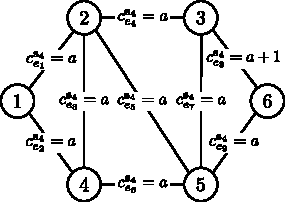
\includegraphics[width=\textwidth]{Chapter_II/MIN-MAX-DESC2-example/a}
		\caption{}
		\label{fig:minmaxexample:a}
	\end{subfigure}
	\hfill
	\begin{subfigure}[b]{0.3\textwidth}
		\includegraphics[width=\textwidth]{Chapter_II/MIN-MAX-DESC2-example/b}
		\caption{}
		\label{fig:minmaxexample:b}
	\end{subfigure}
	\hfill\null
	\caption{
		Dyskretne scenariusze $\textbf{s}_{4}$, $\textbf{s}_{5}$ dla grafu nieskierowanego $G = \left( V, E \right)$, $V = \left\{ 1, 2, \dots, 6 \right\}$, $E = \left\{ e_{i} : i \in \left\{ 1, \dots, 9 \right\} \right\}$.
		Dla tak określonych scenariuszy dłużej już nie zachodzi własność: $\forall e \in E : c^{\textbf{s}_{4}}_{e} \leqslant c^{\textbf{s}_{5}}_{e}$.
	}
	\label{fig:minmaxexample}
\end{figure}

Problem jest tym bardziej widoczny, im większe różnice będą zachodzić pomiędzy poszczególnymi scenariuszami.
Za przykład niech posłuży nam ilustracja \ref{fig:minmaxexample2}, gdzie pomimo występowania nadal jedynie dwóch scenariuszy, opieranie się na dotychczasowej intuicji policzenia optymalnych rozwiązań dla każdego z~nich i~wybraniu jednego, prowadzi do znacznie poważniejszych błędów, niż miało to miejsce w~poprzednim przykładzie, gdzie pomimo zastosowania błędnej logiki, otrzymaliśmy poprawny rezultat.
Wprowadźmy kolejne scenariusze: $\textbf{s}_{6} = \left[ 0, 0, 2^{n}, 2^{n}, 1, 1, 1, 1 \right]$ oraz $\textbf{s}_{7} = \left[ 2^{n}, 2^{n}, 0, 0, 1, 1, 1, 1 \right]$, gdzie $n$ jest dowolne\footnote{
	Chcemy aby funkcje zmiennej $n$ przyjmowały wartość większą od jedynki, co w~przypadku funkcji wykładniczej jest spełnione dla dowolnego $n \in \NN^{+}$.
}.

\begin{figure}[!htbp]
	\null\hfill
	\begin{subfigure}[b]{0.3\textwidth}
		\includegraphics[width=\textwidth]{Chapter_II/MIN-MAX-DESC3-example/a}
		\caption{}
		\label{fig:minmaxexample2:a}
	\end{subfigure}
	\hfill
	\begin{subfigure}[b]{0.3\textwidth}
		\includegraphics[width=\textwidth]{Chapter_II/MIN-MAX-DESC3-example/b}
		\caption{}
		\label{fig:minmaxexample2:b}
	\end{subfigure}
	\hfill\null
	\caption{
		Skrajny przykład problemu \textsc{Discrete Min-Max Spanning Tree}, gdzie optymalne rozwiązania dla poszczególnych scenariuszy okazują się być bardzo złe (dla dużych $n$) w~porównaniu z~rozwiązaniem głównego problemu.
		Podobny przykład~\cite[$429$--$430$]{minmaxSurvey} można skonstruować dla minimaksowego problemu najkrótszej ścieżki.
	}
	\label{fig:minmaxexample2}
\end{figure}

Optymalnymi rozwiązaniami dla poszczególnych scenariuszy są oczywiście: $T^{\ast}_{\textbf{s}_{6}} = \left\{ e_{1}, e_{2}, e_{6}, e_{7} \right\}$, o~całkowitym koszcie równym $2$, oraz $T^{\ast}_{\textbf{s}_{7}} = \left\{ e_{3}, e_{4}, e_{6}, e_{7} \right\}$, gdzie $v \left( \textbf{s}_{7}, x^{\ast}_{\textbf{s}_{7}} \right)$ ma tą samą wartość co poprzednie rozwiązanie\footnote{
	Z oznaczeniem $v \left( \textbf{s}, \textbf{x} \right)$ spotkaliśmy się już wcześniej, przy omawianiu tabeli \ref{tab:minmaxexample}, gdzie wyrażenie to oznaczało całkowity koszt dopuszczalnego rozwiązania problemu optymalizacyjnego dla zadanego scenariusza $\textbf{s}$ oraz wybranego zbioru krawędzi, reprezentowanego przez wektor $\textbf{x}$.
	Analogicznie poprzez $v \left( \textbf{s}, x^{\ast}_{\textbf{s}} \right)$ oznaczać będziemy koszt \textbf{optymalnego} rozwiązania dla scenariusza $\textbf{s}$, gdzie $x^{\ast}_{\textbf{s}}$ to binarny wektor reprezentujący optymalne rozwiązanie dla danego scenariusza ($T^{\ast} = \left\{ e : x_{e} = 1 \right\}$).
	Często będziemy skracać ten zapis do $v^{\ast}_{\textbf{s}}$.}.
Oczywiście po podstawieniu otrzymanych danych do wzoru: $\min_{\textbf{x} \in X^{\ast}} \max_{\textbf{s} \in \mathcal{S}} v \left( \textbf{x}, \textbf{s} \right)$, gdzie $X^{\ast} = \left\{ \textbf{x}^{\ast}_{\textbf{s}_{6}}, \textbf{x}^{\ast}_{\textbf{s}_{7}} \right\}$ otrzymamy:

\begin{equation*}
	\min \left\{ \max_{ \mathclap{\textbf{s} \in \mathcal{S}}} v \left( \textbf{x}^{\ast}_{\textbf{s}_{6}}, \textbf{s} \right), \max_{\mathclap{\textbf{s} \in \mathcal{S}}} v \left( \textbf{x}^{\ast}_{\textbf{s}_{7}}, \textbf{s} \right)  \right\} = \min \left\{ \max \left\{ v \left( \textbf{x}^{\ast}_{\textbf{s}_{6}}, \textbf{s}_{6} \right), v \left( \textbf{x}^{\ast}_{\textbf{s}_{6}}, \textbf{s}_{7} \right) \right\}, \max \left\{ v \left( \textbf{x}^{\ast}_{\textbf{s}_{7}}, \textbf{s}_{6} \right), v \left( \textbf{x}^{\ast}_{\textbf{s}_{7}}, \textbf{s}_{7} \right) \right\} \right\}\text{.}
\end{equation*}

Łatwo zauważyć, że $v \left( \textbf{x}^{\ast}_{\textbf{s}_{6}}, \textbf{s}_{6} \right) < v \left( \textbf{x}^{\ast}_{\textbf{s}_{6}}, \textbf{s}_{7} \right)$ oraz $v \left( \textbf{x}^{\ast}_{\textbf{s}_{7}}, \textbf{s}_{7} \right) < v \left( \textbf{x}^{\ast}_{\textbf{s}_{7}}, \textbf{s}_{6} \right)$. Stąd:

\begin{eqnarray}
	\max \left\{ v \left( \textbf{x}^{\ast}_{\textbf{s}_{6}}, \textbf{s}_{6} \right), v \left( \textbf{x}^{\ast}_{\textbf{s}_{6}}, \textbf{s}_{7} \right) \right\} = v \left( \textbf{x}^{\ast}_{\textbf{s}_{6}}, \textbf{s}_{7} \right) = 2 \cdot 2^{n} + 2 = 2^{n+1} + 2\text{,} \\
	\max \left\{ v \left( \textbf{x}^{\ast}_{\textbf{s}_{7}}, \textbf{s}_{6} \right), v \left( \textbf{x}^{\ast}_{\textbf{s}_{7}}, \textbf{s}_{7} \right) \right\} = v \left( \textbf{x}^{\ast}_{\textbf{s}_{7}}, \textbf{s}_{6} \right) = 2 \cdot 2^{n} + 2 = 2^{n+1} + 2\text{,}
\end{eqnarray}
a całe wyrażenie skraca się do $\min \left\{ 2^{n+1} + 2, 2^{n+1} + 2  \right\} = 2^{n+1} + 2$, podczas gdy optymalną wartością dla problemu \textsc{Min-Max Spanning Tree} dla tych scenariuszy wynosi $v \left( x^{\ast} \right) = v^{\ast} = 4$, gdzie $x^{\ast} = \left[ 0, 0, 0, 0, 1, 1, 1, 1 \right]$ (zbiór $T^{\ast} = \left\{ e_{5}, e_{6}, e_{7}, e_{8} \right\}$).
Uzyskaliśmy zatem błąd rzędu wykładniczego.



\subsection{Sposoby aproksymacji problemu}



Aby nie musieć uciekać się do rozwiązywania problemu \textsc{Min-Max} ze zbiorem scenariuszy $S$ prosto z~definicji tj.

\begin{itemize}
	\item dla każdego dopuszczalnego rozwiązania $\textbf{x} \in X$ wygenerować zbiór $V^{\textbf{x}}_{S} = \left\{ v \left( \textbf{x}, \textbf{s} \right) : \textbf{s} \in S \right\}$ (zawierający wartości rozwiązań dla ustalonego wektora $\textbf{x}$ dla wszystkich scenariuszy w~$S$),
	\item z~tak powstałego zbioru $\mathcal{V}^{X}_{S} = \left\{ \max_{y \in V^{\textbf{x}}_{S}} \left\{ y \right\} : \textbf{x} \in X  \right\}$ wybrać rozwiązanie $\textbf{x}^{\ast} \in X$, dla którego $v \left( \textbf{x}^{\ast}, S \right) = \min_{z \in \mathcal{V}^{X}_{S}} \left\{ z \right\}$,
\end{itemize}
możemy próbować aproksymować problem na podstawie jednego scenariusza, który jest składową wszystkich rozpatrywanych scenariuszy ~\cite{minmaxApprox}~\cite[$430$]{minmaxSurvey}.
Przyjrzyjmy się dwóm podejściom do rozpatrywanego przez nas problemu, w~obu przypadkach otrzymamy jego $k$-aproksymację, gdzie $k$ będzie liczbą scenariuszy, jakie bierzemy pod uwagę.
Choć będziemy skupiać się tylko na problemie \textsc{Min-Max Spanning Tree}, przedstawione dowody da się z~łatwością uogólnić na całą klasę problemów \textsc{Min-Max}.


\subsubsection{Uśrednianie scenariuszy}


Pierwszym, najprostszym do udowodnienia pomysłem jest potraktowanie problemu minimalizacyjnego $\mathcal{P}$ ze zbiorem scenariuszy $S$ ($\left| S \right| = k$) jako problemu z~pojedynczym scenariuszem, zdefiniowanym w~sposób podany w~poniższym twierdzeniu.

\begin{theorem}\label{th:minmaxavg}~\cite[$430$]{minmaxSurvey}
	Niech $\mathcal{I}$ będzie instancją problemu \textsc{Discrete Min-Max $\mathcal{P}$}.
	Niech problem zawiera $k$ scenariuszy w~zbiorze $S$ i~niech każdy $\textbf{s}_{j} \in S$ będzie zdefiniowany jako $\textbf{s}_{j} = \left[ c^{\textbf{s}_{j}}_{1}, \dots, c^{\textbf{s}_{j}}_{m} \right]$.
	Dodatkowo niech $\mathcal{I^{\prime}}$ będzie instancją problemu $\mathcal{P}$ z~jednym scenariuszem $\textbf{s}^{\prime}$, którego koszty są średnią kosztów scenariuszy $\textbf{s} \in S$.
	Wtedy, jeżeli istnieje optymalne rozwiązanie $\textbf{x}^{\prime}$ dla $\mathcal{I}^{\prime}$, to $\max_{\textbf{s} \in S} v \left( \textbf{x}^{\prime}, \textbf{s} \right) \leqslant k \cdot opt \left( \mathcal{I} \right)$, gdzie $opt \left( \mathcal{I} \right)$ oznacza optymalną wartość rozwiązania dla $\mathcal{I}$.
\end{theorem}

\begin{proof}~\cite[$430$]{minmaxSurvey}
	Koszty scenariusza $\textbf{s}^{\prime}$ dla $\mathcal{I}^{\prime}$ są zdefiniowane następująco:
	\begin{equation}
		c^{\textbf{s}^{\prime}}_{i} = \sum_{\mathclap{j = 1}}^{k} \frac{c_{i}^{\textbf{s}_{j}}}{k} \qquad \forall i \in \left\{ 1, \dots, m \right\}\text{.}
	\end{equation}
	
	Rozpisując wyrażenie $v \left( \textbf{x}, \textbf{s}^{\prime} \right) = \sum_{e \in E} x_{e} \cdot c^{\textbf{s}^{\prime}}_{e}$ otrzymujemy: $\sum_{e \in E} x_{e} \cdot \left( \sum_{j = 1}^{k} \frac{c_{e}^{\textbf{s}_{j}}}{k} \right) = \frac{1}{k} \cdot \sum_{j = 1}^{k} \sum_{e \in E} x_{e} \cdot c^{\textbf{s}_{j}}_{e} = \frac{1}{k} \cdot \sum_{\textbf{s} \in S} v \left( \textbf{x}, \textbf{s} \right)$.
	Pokażemy, że optymalne rozwiązanie $\textbf{x}^{\prime}$ dla scenariusza $\textbf{s}^{\prime}$ nie jest gorsze od optymalnego rozwiązania oryginalnego problemu (w przeciwnym wypadku rozważanie takiego scenariusza byłoby bezcelowe, gdyż nawet jego optymalne rozwiązanie było by gorsze od pożądanego).
	Mamy zatem:
	
	\begin{equation}
		L = v \left( \textbf{x}^{\prime}, \textbf{s}^{\prime} \right) = \min_{\mathclap{\textbf{x} \in X}} v \left( \textbf{x}, \textbf{s}^{\prime} \right) = \min_{ \mathclap{\textbf{x} \in X}} \frac{1}{k} \cdot \sum_{\textbf{s} \in S} v \left( \textbf{x}, \textbf{s} \right) \leqslant \min_{ \mathclap{\textbf{x} \in X}} \frac{1}{k} \cdot k \cdot \max_{\textbf{s} \in S} v \left( \textbf{x}, \textbf{s} \right) = \min_{ \mathclap{\textbf{x} \in X}} \max_{\textbf{s} \in S} v \left( \textbf{x}, \textbf{s} \right) = opt \left( \mathcal{I}\right)\text{.}
	\end{equation}
	
	W czasie obliczeń skorzystaliśmy z~własności $\sum_{\textbf{s} \in S} v \left( \textbf{x}, \textbf{s} \right) \leqslant k \cdot \max_{\textbf{s} \in S} v \left( \textbf{x}, \textbf{s} \right)$ (liczba scenariuszy $\left| S \right| = k$).
	Wartość $L$ nazywamy \textbf{dolnym ograniczeniem}.
	\textbf{Górnym ograniczeniem} na wartość rozwiązania jest oczywiście $\max_{\textbf{s} \in S} v \left( \textbf{x}^{\prime}, \textbf{s} \right) = U$.
	Próbując ograniczać otrzymaną wartość $U$ otrzymamy:
	
	\begin{eqnarray}
		opt \left( \mathcal{I} \right) = \min_{ \mathclap{\textbf{x} \in X}} \max_{\textbf{s} \in S} v \left( \textbf{x}, \textbf{s} \right) \leqslant \max_{\textbf{s} \in S} v \left( \textbf{x}^{\prime}, \textbf{s} \right) \leqslant \sum_{\textbf{s} \in S} v \left( \textbf{x}^{\prime}, \textbf{s} \right) = k \cdot \frac{1}{k} \cdot \sum_{\textbf{s} \in S} v \left( \textbf{x}^{\prime}, \textbf{s} \right) = k \cdot L \leqslant k \cdot opt \left( \mathcal{I} \right)\text{,}
	\end{eqnarray}
	gdzie w~dwóch ostatnich równościach skorzystaliśmy z~tego, że $L = \min_{ \textbf{x} \in X} \frac{1}{k} \cdot \sum_{\textbf{s} \in S} v \left( \textbf{x}, \textbf{s} \right) = \frac{1}{k} \cdot \sum_{\textbf{s} \in S} v \left( \textbf{x}^{\prime}, \textbf{s} \right)$ oraz, że wcześniej udowodniliśmy nierówność $L \leqslant opt \left( \mathcal{I} \right)$.
	Pokazaliśmy zatem, że $\max_{\textbf{s} \in S} v \left( \textbf{x}^{\prime}, \textbf{s} \right) \leqslant k \cdot opt \left( \mathcal{I} \right)$, co oznacza, że wybierając optymalne rozwiązanie $\textbf{x}^{\prime}$ dla scenariusza $\textbf{s}^{\prime}$, w~najgorszym możliwym przypadku (wystąpienia takiego scenariusza, że wartość rozwiązania dla wybranego $\textbf{x}^{\prime}$ będzie najbardziej oddalona od minimum) otrzymane rozwiązanie nie będzie gorsze niż $k$-krotność wartości optymalnej.
\end{proof}


\subsubsection{Scenariusz najgorszych wartości}


Scenariuszem najgorszych wartości będziemy nazywać taki scenariusz, którego każdy koszt, który definiuje, jest największym z~możliwych, odpowiadających mu, kosztów scenariuszy, z~których ten scenariusz powstaje.
Innymi słowy, powracając do rysunku \ref{fig:minmaxexample2}, jeżeli mamy dwa scenariusze: $\textbf{s}_{6} = \left[ 0, 0, 2^{n}, 2^{n}, 1, 1, 1, 1 \right]$ oraz $\textbf{s}_{7} = \left[ 2^{n}, 2^{n}, 0, 0, 1, 1, 1, 1 \right]$, to scenariuszem najgorszych wartości będzie scenariusz $s^{\prime} = \left[ 2^{n}, 2^{n}, 2^{n}, 2^{n}, 1, 1, 1, 1 \right]$~--- tak samo jak w~przypadku ciągłym, gdy najgorszy z~możliwych scenariuszy był definiowany za pomocą $\overline{s}$, tak wszystkie koszty scenariusza $s^{\prime}$ są nie mniejsze niż odpowiadające im wartości w~scenariuszach pozostałych.
Co więcej, jeżeli wykorzystalibyśmy tak stworzony scenariusz $s^{\prime}$ do rozwiązania problemu przedstawionego na ilustracji \ref{fig:minmaxexample2}, otrzymalibyśmy rozwiązanie optymalne, podobnie jak miałoby to miejsce w~przypadku ciągłym.
Pokażemy jednak, że~--- pomimo obiecującego wyniku~--- taka próba podejścia do problemów \textsc{Min-Max} nie zapewnia nam optymalnego rozwiązania, a~co najwyżej jego $k$-aproksymację, podobnie jak poprzednio zaprezentowana metoda.

\begin{theorem}\label{th:minmaxworst}~\cite[$430$]{minmaxSurvey}
	Niech $\mathcal{I}$ będzie instancją problemu \textsc{Discrete Min-Max $\mathcal{P}$}.
	Niech problem zawiera $k$ scenariuszy w~zbiorze $S$ i~niech każdy $\textbf{s} \in S$ będzie zdefiniowany jako $\textbf{s} = \left[ c^{\textbf{s}}_{1}, \dots, c^{\textbf{s}}_{m} \right]$.
	Dodatkowo niech $\mathcal{I^{\prime}}$ będzie instancją problemu $\mathcal{P}$ z~pojedynczym scenariuszem najgorszych wartości $\textbf{s}^{\prime}$.
	Wtedy, jeżeli istnieje optymalne rozwiązanie $\textbf{x}^{\prime}$ dla $\mathcal{I}^{\prime}$, to $\max_{\textbf{s} \in S} v \left( \textbf{x}^{\prime}, \textbf{s} \right) \leqslant k \cdot opt \left( \mathcal{I} \right)$, gdzie $opt \left( \mathcal{I} \right)$ oznacza optymalną wartość rozwiązania dla $\mathcal{I}$.
\end{theorem}

\begin{proof}~\cite[$430$]{minmaxSurvey}
	Koszty scenariusza $\textbf{s}^{\prime}$ dla $\mathcal{I}^{\prime}$ są zdefiniowane następująco:
	
	\begin{equation}
		c^{\textbf{s}^{\prime}}_{i} = \max_{\mathclap{\textbf{s} \in S}} c^{\textbf{s}}_{i} \qquad \forall i \in \left\{ 1, \dots, m \right\}\text{.}
	\end{equation}
	
	Pokażemy ciąg przekształceń, który da nam górne oszacowanie na wartość wyrażenia $ \max_{\textbf{s} \in S} v \left( \textbf{x}^{\prime}, \textbf{s} \right)$.
	Niech $\textbf{x}^{\ast}$ będzie optymalnym rozwiązaniem oryginalnego problemu $\mathcal{I}$:
	
	\begin{equation}
		\max_{\mathclap{\textbf{s} \in S}} v \left( \textbf{x}^{\prime}, \textbf{s} \right) \leqslant \sum_{\mathclap{i = 1}}^{m} c_{i}^{\textbf{s}^{\prime}} \cdot x_{i}^{\prime} \leqslant \sum_{\mathclap{i = 1}}^{m} c_{i}^{\textbf{s}^{\prime}} \cdot x_{i}^{\ast} \leqslant \sum_{\mathclap{i = 1}}^{m} \sum_{\mathclap{\textbf{s} \in S}} c_{i}^{\textbf{s}} \cdot x_{i}^{\ast} =  \sum_{\mathclap{\textbf{s} \in S}} \sum_{\mathclap{i = 1}}^{m} c_{i}^{\textbf{s}} \cdot x_{i}^{\ast} \leqslant k \cdot \max_{\mathclap{\textbf{s} \in S}} \sum_{\mathclap{i = 1}}^{m} c_{i}^{\textbf{s}} \cdot x_{i}^{\ast} = k \cdot opt \left( \mathcal{I} \right)\text{.}
	\end{equation}
	
	Chcąc dokładniej przyjrzeć się przeprowadzonemu przez nas rozumowaniu:
	
	\begin{itemize}
		\item $\max_{\textbf{s} \in S} v \left( \textbf{x}^{\prime}, \textbf{s} \right) = \sum_{i = 1}^{m} c_{i}^{\textbf{s}} \cdot x_{i}^{\prime} \leqslant \sum_{i = 1}^{m} c_{i}^{\textbf{s}^{\prime}} \cdot x_{i}^{\prime}$ otrzymujemy prosto z~definicji kosztów scenariusza $s^{\prime}$~--- dla każdego $i \in \left\{ 1, \dots, m \right\}$ zachodzi $c_{i}^{\textbf{s}} \leqslant \max_{\textbf{s} \in S} c^{\textbf{s}}_{i} = c_{i}^{\textbf{s}^{\prime}}$, zaś reszta wyrażenia nie ulega zmianie,
		\item $\sum_{i = 1}^{m} c_{i}^{\textbf{s}^{\prime}} \cdot x_{i}^{\prime} \leqslant \sum_{i = 1}^{m} c_{i}^{\textbf{s}^{\prime}} \cdot x_{i}^{\ast}$~--- rozwiązanie, opisywane przez wektor $\textbf{x}^{\prime}$, jest optymalne dla scenariusza z~kosztami $c_{i}^{\textbf{s}^{\prime}}$, zatem każde inne rozwiązanie jest nie lepsze od niego ($\textbf{x}^{\ast}$ jest optymalne dla kosztów oryginalnych, nie dla tych, które występują w~nierówności),
		\item $\sum_{i = 1}^{m} c_{i}^{\textbf{s}^{\prime}} \cdot x_{i}^{\ast} \leqslant \sum_{i = 1}^{m} \sum_{\textbf{s} \in S} c_{i}^{\textbf{s}} \cdot x_{i}^{\ast}$ w~oczywisty sposób wynika z~faktu, że dla każdego $i \in \left\{ 1, \dots, m \right\}$ zachodzi $c_{i}^{\textbf{s}^{\prime}} = \max_{\textbf{s} \in S} c^{\textbf{s}}_{i} \leqslant \sum_{\textbf{s} \in S} c^{\textbf{s}}_{i}$,
		\item $\max_{\textbf{s} \in S} \sum_{i = 1}^{m} c_{i}^{\textbf{s}} \cdot x_{i}^{\ast}$ jest równe wartości rozwiązania dla najgorszego możliwego przypadku, zakładając, że podstawiane do wzoru rozwiązanie $\textbf{x}^{\ast}$ jest optymalne~--- $ opt \left( \mathcal{I} \right)$.
	\end{itemize}
	
	Pokazaliśmy zatem, tak samo jak w~przypadku poprzedniego twierdzenia, że takie podejście do problemu \textsc{Min-Max} zapewnia nam jedynie $k$-aproksymację rozwiązania.
\end{proof}




\section{Problemy minimaksowe ze względną funkcją optymalności}




W poprzednim dziale rozważaliśmy problem, który możemy najłatwiej określić pytaniem: ,,Jakie wybrać rozwiązanie, aby w~najgorszym przypadku było ono najlepsze z~możliwych?''.
Skupiało się zatem ono tylko na niwelowaniu strat, których można było się spodziewać, nie zaś na faktycznym szukaniu rozwiązania, które byłoby możliwie bliskie optymalnego.
W~tym podrozdziale zmienimy nieco nasze podejście do postawionego problemu i~zadamy sobie pytanie: ,,Jakie rozwiązanie wybrać, aby w~najgorszym przypadku było ono tak blisko rozwiązania optymalnego, jak to tylko możliwe?''.
Aby to osiągnąć, wprowadzimy pojęcie \textbf{żalu} (ang. \textit{regret}).
Niech $v_{\textbf{s}}^{\ast}$ oznacza wartość optymalnego rozwiązania dla scenariusza $\textbf{s}$.
Wektorem zapewniającym to rozwiązanie optymalne, jest wektor $x^{\ast}_{\textbf{s}}$.
Oznacza to, że dla każdego innego wektora $\textbf{x} \neq \textbf{x}^{\ast}_{\textbf{s}}$ zachodzi $v \left( \textbf{x}, \textbf{s} \right) \geqslant v \left( \textbf{x}^{\ast}_{\textbf{s}}, \textbf{s} \right)$.
Różnicę tych dwóch wartości nazywamy żalem i~reprezentuje on stratę, jaką ponieśliśmy w~konsekwencji wyboru innego rozwiązania niż optymalne dla danego scenariusza.
Istotą problemu \textsc{Min-Max Regret}~\cite[$595$]{Kasperski2012} jest wybranie takiego rozwiązania $\textbf{x}$, aby zminimalizować tę różnicę dla wszystkich scenariuszy, w~szczególności dla tego najgorszego, bo to od niego zależy wynik poniższego wyrażenia:

\begin{equation}
	\min_{\mathclap{\textbf{x} \in X}} \max_{\mathclap{\textbf{s} \in S}} \left( v \left( \textbf{x}, \textbf{s} \right) - v \left( \textbf{x}^{\ast}_{\textbf{s}}, \textbf{s} \right) \right)\text{.}
\end{equation}

Możemy także rozpatrywać przypadek \textsc{Max-Min Regret}, którego definicja nieco różni się od tej podanej wyżej i~nie jest analogiczna do problemu \textsc{Max-Min}: $\min_{\textbf{x} \in X} \max_{\textbf{s} \in S} \left( v \left( \textbf{x}^{\ast}_{\textbf{s}}, \textbf{s} \right) - v \left( \textbf{x}, \textbf{s} \right) \right)$.
Tak samo jak w~przypadku poprzednich problemów, tutaj też możemy wyróżnić podział na scenariusze ciągłe oraz dyskretne.



\subsection{Przypadek dyskretny}



Tym razem zaczniemy od omówienia przypadku dyskretnego, gdyż~--- jak się będziemy mogli przekonać~--- wiele z~tego, co do tej pory powiedzieliśmy o~problemach \textsc{Min-Max}, powtórzy się dla problemów \textsc{Min-Max Regret}.
Podobnie jak to miało miejsce w~przypadku poprzedniej klasy problemów, zaczniemy od omówienia prostego przykładu, który przedstawia rysunek \ref{fig:minmaxregexample}, a~na którym zaznaczono optymalne rozwiązania dla problemu \textsc{Min-Max Regret Minimum Spanning Tree} dla dwóch scenariuszy: $\textbf{s}_{1}$ oraz $\textbf{s}_{2}$, natomiast w~tabeli \ref{tab:minmaxregexample2}~--- $7$ przykładowych wyników, jakie daje zastosowanie różnych drzew rozpinających.
Już dwa pierwsze rozwiązania: $\textbf{x}_{1}$ oraz $\textbf{x}_{2}$ wskazują na to, że kierowanie się przy wyborze rozwiązania dla tego problemu tylko kryterium optymalności dla pojedynczego scenariusza jest błędne i~nie należy go stosować; obydwa rozwiązania są optymalne odpowiednio dla scenariuszy $\textbf{s}_{1}$ oraz $\textbf{s}_{2}$, lecz nie dają tego samego rezultatu przy rozpatrywaniu właściwego problemu.

\begin{figure}[!htbp]
	\null\hfill
	\begin{subfigure}[b]{0.35\textwidth}
		\includegraphics[width=\textwidth]{Chapter_II/MIN-MAX-REG-example/a}
		\caption{}
		\label{fig:minmaxregexample:a}
	\end{subfigure}
	\hfill
	\begin{subfigure}[b]{0.35\textwidth}
		\includegraphics[width=\textwidth]{Chapter_II/MIN-MAX-REG-example/b}
		\caption{}
		\label{fig:minmaxregexample:b}
	\end{subfigure}
	\hfill\null
	\caption{
		Dyskretne scenariusze $\textbf{s}_{1}$, $\textbf{s}_{2}$ dla grafu nieskierowanego $G = \left( V, E \right)$, $V = \left\{ 1, 2, \dots, 6 \right\}$, $E = \left\{ e_{i} : i \in \left\{ 1, \dots, 9 \right\} \right\}$.
		\textbf{(a)}~Optymalnym rozwiązaniem dla scenariusza $\textbf{s}_{1}$ jest zbiór wierzchołków $T^{\ast}_{\textbf{s}_{1}} = \left\{ e_{1}, e_{3}, e_{4}, e_{6}, e_{9} \right\}$, któremu odpowiada wektor $\textbf{x}^{\ast}_{\textbf{s}_{1}} = \left[ 1, 0, 1, 1, 0, 1, 0, 0, 1 \right]$.
		Wartość tego rozwiązania wynosi $v^{\ast}_{\textbf{s}_{1}} = 11$.
		\textbf{(b)}~Optymalnym rozwiązaniem dla scenariusza $\textbf{s}_{2}$ jest zbiór wierzchołków $T^{\ast}_{\textbf{s}_{2}} = \left\{ e_{1}, e_{3}, e_{4}, e_{6}, e_{8} \right\}$, któremu odpowiada wektor $\textbf{x}^{\ast}_{\textbf{s}_{2}} = \left[ 1, 0, 1, 1, 0, 1, 0, 1, 0 \right]$.
		Wartość tego rozwiązania wynosi $v^{\ast}_{\textbf{s}_{2}} = 25$.
	}
	\label{fig:minmaxregexample}
\end{figure}

\begin{table}[!htbp]
	\caption{
		Tabela przedstawiająca część z~osiągalnych rozwiązań dla problemu minimalnego drzewa rozpinającego dla scenariuszy $\textbf{s}_{1}$ oraz $\textbf{s}_{2}$ (\ref{fig:minmaxregexample:a} i~\ref{fig:minmaxregexample:b}), koszty dla każdego z~proponowanych rozwiązań dla podanych scenariuszy, poniesione straty względem optymalnych rozwiązań oraz wartość rozwiązania dla problemu \textsc{Min-Max Regret}.
		Wiersze w~tabeli zostały posortowane w~kolejności rosnących wartości rozwiązań.
	}
	\label{tab:minmaxregexample2}
	\centering
	\begin{tabular}{ccccccccccccccc}
		\cline{11-15}
		\multicolumn{2}{c}{}       &         &         &         &         &         &         &         &         & \multicolumn{5}{c}{Scenariusze}                                                                                                                                                                                             \\ \hline
		$X$              & $e_{1}$ & $e_{2}$ & $e_{3}$ & $e_{4}$ & $e_{5}$ & $e_{6}$ & $e_{7}$ & $e_{8}$ & $e_{9}$ & $v \left( \textbf{x}, \textbf{s}_{1} \right) $ & $r_{\textbf{s}_{1}}$  & $v \left( \textbf{x}, \textbf{s}_{2} \right) $ &  $r_{\textbf{s}_{2}}$ & $\max \left\{ r_{\textbf{s}_{1}}, r_{\textbf{s}_{2}} \right\} $ \\ \hline
		$\textbf{x}_{1}$ & $1$     & $0$     & $1$     & $1$     & $0$     & $1$     & $0$     & $0$	&	$1$	&	$11$	&	$0$	&	$26$	&	$1$	&	$1$	\\
		$\textbf{x}_{2}$ & $1$     & $0$     & $1$     & $1$     & $0$     & $1$     & $0$     & $1$	&	$0$	&	$13$	&	$2$	&	$25$	&	$0$	&	$2$	\\
		$\textbf{x}_{3}$ & $1$     & $0$     & $1$     & $0$     & $0$     & $1$     & $0$     & $1$	&	$1$	&	$13$	&	$2$	&	$26$	&	$1$	&	$2$	\\
		$\textbf{x}_{4}$ & $1$     & $0$     & $1$     & $0$     & $0$     & $1$     & $1$     & $0$	&	$1$	&	$12$	&	$1$	&	$28$	&	$3$	&	$3$	\\
		$\dots$ & $\dots$     & $\dots$     & $\dots$     & $\dots$     & $\dots$     & $\dots$     & $\dots$     & $\dots$	&	$\dots$	&	$\dots$	&	$\dots$	&	$\dots$	&	$\dots$	&	$\dots$	\\
		$\textbf{x}_{53}$ & $0$     & $1$     & $1$     & $0$     & $1$     & $0$     & $1$     & $1$	&	$0$	&	$25$	&	$14$	&	$35$	&	$10$	&	$14$	\\
		$\textbf{x}_{54}$ & $0$     & $1$     & $0$     & $0$     & $1$     & $1$     & $1$     & $1$	&	$0$	&	$26$	&	$15$	&	$38$	&	$13$	&	$15$	\\
		$\textbf{x}_{55}$ & $1$     & $1$     & $0$     & $0$     & $1$     & $0$     & $1$     & $1$	&	$0$	&	$26$	&	$15$	&	$37$	&	$12$	&	$15$	\\
		\hline
	\end{tabular}
\end{table}

\begin{figure}[!htbp]
	\null\hfill
	\begin{subfigure}[b]{0.3\textwidth}
		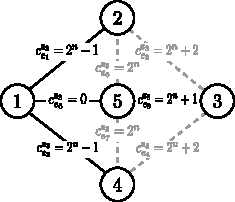
\includegraphics[width=\textwidth]{Chapter_II/MIN-MAX-REG2-example/a}
		\caption{}
		\label{fig:minmaxregexample2:a}
	\end{subfigure}
	\hfill
	\begin{subfigure}[b]{0.3\textwidth}
		\includegraphics[width=\textwidth]{Chapter_II/MIN-MAX-REG2-example/b}
		\caption{}
		\label{fig:minmaxregexample2:b}
	\end{subfigure}
	\hfill
	\begin{subfigure}[b]{0.3\textwidth}
		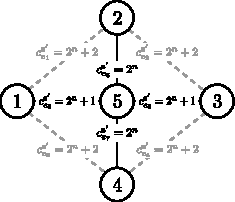
\includegraphics[width=\textwidth]{Chapter_II/MIN-MAX-REG2-example/c}
		\caption{}
		\label{fig:minmaxregexample2:c}
	\end{subfigure}
	\hfill\null
	\caption{
		Dyskretne scenariusze $\textbf{s}_{3}$, $\textbf{s}_{4}$ i~$\textbf{s}^{\prime}$ dla grafu nieskierowanego $G = \left( V, E \right)$, $V = \left\{ 1, 2, \dots, 5 \right\}$, $E = \left\{ e_{i} : i \in \left\{ 1, \dots, 8 \right\} \right\}$, gdzie $\textbf{s}^{\prime}$ jest sztucznie wygenerowanym scenariuszem najgorszych kosztów.
		\textbf{(a)}~Optymalne rozwiązanie $T^{\ast}_{\textbf{s}_{3}} = \left\{ e_{1}, e_{3}, e_{5}, e_{8} \right\}$ o~całkowitym koszcie $3 \cdot 2^{n} - 1$.
		\textbf{(b)}~Optymalne rozwiązanie $T^{\ast}_{\textbf{s}_{4}} = \left\{ e_{2}, e_{4}, e_{5}, e_{8} \right\}$ o~identycznym koszcie, co $v^{\ast}_{\textbf{s}_{3}}$.
		\textbf{(c)}~Optymalne rozwiązanie dla scenariusza $\textbf{s}^{\prime}$ o~kosztach $c_{i}^{\textbf{s}^{\prime}} = \max_{\textbf{s} \in S} c_{i}^{\textbf{s}}$.
		Koszt całkowity rozwiązania optymalnego wynosi $v \left( \textbf{x}^{\ast}_{\textbf{s}^{\prime}}, \textbf{s}^{\prime} \right) = 4 \cdot 2^{n} + 2$.
	}
	\label{fig:minmaxregexample2}
\end{figure}


\subsubsection{Aproksymacja rozwiązania}


Chcąc otrzymać aproksymację dla problemu \textsc{Min-Max Regret}, możemy odwołać się do udowodnionego twierdzenia \ref{th:minmaxavg}~--- jego dowód przebiega analogicznie dla tej klasy problemów~\cite[propozycja $1$]{minmaxSurvey} i~zostanie tu pominięty.
Dużo ciekawszy okazuje się natomiast przypadek, w~którym tworzyliśmy dodatkowy scenariusz $s^{\prime}$, którego koszty definiowaliśmy jako $c^{\prime}_{i} = \max_{\textbf{s} \in S} c^{\textbf{s}}_{i} \; \forall i \in \left\{ 1, \dots, m \right\}$.
Pokażemy, że nawet dla dwóch scenariuszy (gdzie spodziewalibyśmy się wyniku co najwyżej $2$ razy gorszego niż optymalny) otrzymany rezultat jest dalece gorszy od spodziewanego.
Stwórzmy dwa scenariusze: $\textbf{s}_{3} = \left[ 2^{n} - 1, 2^{n} + 2, 2^{n} - 1, 2^{n} + 2, 0, 2^{n}, 2^{n}, 2^{n} + 1 \right]$ oraz $\textbf{s}_{4} = \left[ 2^{n} + 2, 2^{n} - 1, 2^{n} + 2, 2^{n} - 1, 2^{n} + 1, 2^{n}, 2^{n}, 0 \right]$, tak jak na rysunku \ref{fig:minmaxregexample2}.
Będziemy chcieli pokazać, że optymalna wartość rozwiązania problemu \textsc{Min-Max Regret Minimum Spanning Tree} dla takiej konfiguracji scenariuszy wynosi $0$, toteż każda inna wartość (różna od zera), jaką otrzymamy przy rozwiązywaniu problemu z~wykorzystaniem scenariusza $\textbf{s}^{\prime}$, będzie błędna (zgodnie z~twierdzeniem \ref{th:minmaxworst}: $\max_{\textbf{s} \in S} v \left( \textbf{x}^{\prime}, \textbf{s} \right) \leqslant k \cdot opt \left( \mathcal{I} \right)$, zatem w~przypadku, gdy $opt \left( \mathcal{I} \right) = 0$, gdzie $\mathcal{I}$ to instancja oryginalnego problemu, jedyne rozwiązanie $\textbf{x}^{\prime}$ dla scenariusza $\textbf{s}^{\prime}$, które spełnia tą nierówność, także musi mieć wartość równą $0$)\footnote{
	Rozpatrywane przez nas grafy nie posiadają ujemnych wag krawędzi.
}. 

Jak łatwo zauważyć, koszty obydwu scenariuszy dla problemu zostały tak dobrane, aby oba optymalne rozwiązania dla każdego scenariusza nie różniły się pod względem wartości, która wynosi $v^{\ast}_{\textbf{s}_{3}} = v^{\ast}_{\textbf{s}_{4}} = 3 \cdot 2^{n} - 1$.
Jest to o~tyle istotne, że podstawiając te dane do ogólnego wzoru, otrzymujemy:

\begin{equation}\label{eq:minmaxreg}
	\min_{\textbf{x} \in X} \max_{\textbf{s} \in \left\{ \textbf{s}_{3}, \textbf{s}_{4} \right\}} v \left( \textbf{x}, \textbf{s} \right) - v \left( \textbf{x}^{\ast}_{\textbf{s}}, \textbf{s} \right) = \min \left\{   \max_{\textbf{s} \in \left\{ \textbf{s}_{3}, \textbf{s}_{4} \right\}} v \left( \textbf{x}^{\ast}_{\textbf{s}_{3}}, \textbf{s} \right) - v \left( \textbf{x}^{\ast}_{\textbf{s}}, \textbf{s} \right), \max_{\textbf{s} \in \left\{ \textbf{s}_{3}, \textbf{s}_{4} \right\}} v \left( \textbf{x}^{\ast}_{\textbf{s}_{4}}, \textbf{s} \right) - v \left( \textbf{x}^{\ast}_{\textbf{s}}, \textbf{s} \right) \right\}\text{.}
\end{equation}

Na tym etapie możemy zauważyć, że bez względu na to, które rozwiązanie wybierzemy (czy $\textbf{x}^{\ast}_{\textbf{s}_{3}}$ czy $\textbf{x}^{\ast}_{\textbf{s}_{4}}$), dla obu rozpatrywanych scenariuszy otrzymamy identyczną wartość żalu (równą zeru).
Podstawiając dane do wzoru \ref{eq:minmaxreg}, otrzymamy zatem: $\min \left\{ \max \left\{ 0, 0 \right\} , \max \left\{ 0, 0 \right\} \right\} = 0$.
Innych rozwiązań nie rozpatrywaliśmy, gdyż z~samej definicji problemu \textsc{Min-Max Regret} wynika, że $\forall x \in X \; v \left( \textbf{x}, \textbf{s} \right) - v \left( \textbf{x}^{\ast}_{\textbf{s}}, \textbf{s} \right) \geqslant 0$, toteż wartości otrzymane dla pozostałych rozwiązań z~pewnością nie mogą być lepsze.

Zakładając, że analogiczne do \ref{th:minmaxworst} twierdzenie dla \textsc{Min-Max Regret} jest prawdziwe, spodziewamy się, że wartość optymalnego rozwiązania dla dodatkowego scenariusza $\textbf{s}^{\prime}$ będzie nie gorsza niż $k$-krotność powyżej otrzymanego rozwiązania (będzie równa $0$).
Z~rysunku \ref{fig:minmaxregexample2:c} natomiast jednoznacznie wynika, że rozwiązaniem dla tego scenariusza jest zbiór krawędzi $T^{\ast}_{\textbf{s}^{\prime}} = \left\{ e_{5}, e_{6}, e_{7}, e_{8} \right\}$ o~całkowitym koszcie równym $2^{n+2} + 2$, gdzie $\textbf{x}^{\ast}_{\textbf{s}^{\prime}} = \left[ 0, 0, 0, 0, 1, 1, 1, 1 \right]$, zaś po podstawieniu danych do wzoru otrzymamy:

\begin{gather*}
	\min_{\textbf{x} \in \left\{ x^{\ast}_{\textbf{s}^{\prime}} \right\}} \max_{\textbf{s} \in \left\{ \textbf{s}_{3}, \textbf{s}_{4} \right\}} v \left( \textbf{x}, \textbf{s} \right) - v \left( \textbf{x}^{\ast}_{\textbf{s}}, \textbf{s} \right) = \max_{\textbf{s} \in \left\{ \textbf{s}_{3}, \textbf{s}_{4} \right\}} v \left( x^{\ast}_{\textbf{s}^{\prime}}, \textbf{s} \right) - v \left( \textbf{x}^{\ast}_{\textbf{s}}, \textbf{s} \right) = \\ 
	= \max \left\{ v \left( x^{\ast}_{\textbf{s}^{\prime}}, \textbf{s}_{3} \right), v \left( x^{\ast}_{\textbf{s}^{\prime}}, \textbf{s}_{4} \right) \right\} - \left( 3 \cdot 2^{n} - 1 \right) = \max \left\{ 3 \cdot 2^{n} + 1, 3 \cdot 2^{n} + 1 \right\} - 3 \cdot 2^{n} + 1 = 2\text{.}
\end{gather*}

Wynikiem możemy dowolnie manipulować~--- przykładem takiej manipulacji są scenariusze $\textbf{s}^{\prime}_{3}$, $\textbf{s}^{\prime}_{4}$ oraz $\textbf{s}^{\prime\prime}$, przedstawione (wraz z~optymalnymi rozwiązaniami dla każdego z~nich) na rysunkach \ref{fig:minmaxregexample3:a}, \ref{fig:minmaxregexample3:b} i~\ref{fig:minmaxregexample3:c}, gdzie optymalną wartością rozwiązania problemu \textsc{Min-Max Regret} dla tych pierwszych jest ponownie wartość $0$, zaś dla trzeciego z~nich: $2^{n+1} \cdot \left( 2^{n} - 1\right)$.

\begin{figure}[!htbp]
	\null\hfill
	\begin{subfigure}[b]{0.3\textwidth}
		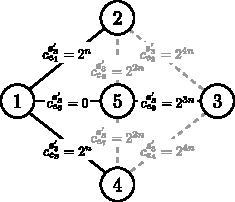
\includegraphics[width=\textwidth]{Chapter_II/MIN-MAX-REG3-example/a}
		\caption{}
		\label{fig:minmaxregexample3:a}
	\end{subfigure}
	\hfill
	\begin{subfigure}[b]{0.3\textwidth}
		\includegraphics[width=\textwidth]{Chapter_II/MIN-MAX-REG3-example/b}
		\caption{}
		\label{fig:minmaxregexample3:b}
	\end{subfigure}
	\hfill
	\begin{subfigure}[b]{0.3\textwidth}
		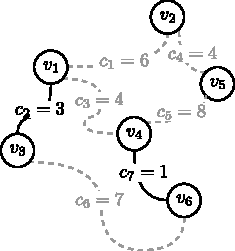
\includegraphics[width=\textwidth]{Chapter_II/MIN-MAX-REG3-example/c}
		\caption{}
		\label{fig:minmaxregexample3:c}
	\end{subfigure}
	\hfill\null
	\caption{
		Scenariusze $\textbf{s}_{3}^{\prime}$ i~$\textbf{s}_{4}^{\prime}$, dla których scenariusz najgorszych kosztów $\textbf{s}^{\prime\prime}$ daje bardzo złe rozwiązanie.
		\textbf{(a)}~Minimalne drzewo rozpinające dla scenariusza $\textbf{s}_{3}^{\prime}$ o~całkowitym koszcie $v^{\ast}_{\textbf{s}_{3}^{\prime}} = 2^{3n} + 2 \cdot 2^{n}$.
		\textbf{(b)}~Minimalne drzewo rozpinające dla scenariusza $\textbf{s}_{4}^{\prime}$ o~takim samym koszcie.
		\textbf{(c)}~Optymalne drzewo rozpinające dla scenariusza $\textbf{s}^{\prime\prime}$.
	}
	\label{fig:minmaxregexample3}
\end{figure}

Pokazaliśmy zatem, że w~tym przypadku nie możemy zastosować analogicznego twierdzenia.



\subsection{Przypadek ciągły}



Zacznijmy od następującego twierdzenia:

\begin{theorem}\label{th:intminmaxreg}~\cite[$431$]{minmaxSurvey}
	Niech dany będzie problem minimalizacyjny $\mathcal{P}$.
	Niech $\underline{\textbf{s}}$ i~$\overline{\textbf{s}}$ będą krytycznymi scenariuszami (odpowiednio najgorszym i~najlepszym), definiującymi przestrzeń scenariuszy $S$.
	Wartość żalu dla dowolnego rozwiązania $\textbf{x} \in X$ jest największa dla, zależnego od $\textbf{x}$, scenariusza $\textbf{s}^{-} \left( \textbf{x} \right)$, którego koszty są zdefiniowane następująco:
	
	\begin{equation}
		c^{\textbf{s}^{-} \left( \textbf{x} \right)}_{i} = \left\{\begin{matrix}
			c^{\overline{\textbf{s}}}_{i} & \text{gdy $e_{i}$ należy do rozwiązania ($x_{i} = 1$),}\\ 
			c^{\underline{\textbf{s}}}_{i} &  \text{w przeciwnym przypadku ($x_{i} = 0$),}
		\end{matrix}\right. \qquad \forall i \in \left\{ 1, 2, \dots, m \right\}\text{.}
	\end{equation}
\end{theorem}

\begin{proof}~\cite[$431$]{minmaxSurvey}
	Dla danego rozwiązania $\textbf{x} \in X$ niech będzie dany zbiór $\mathbb{1} \left( \textbf{x} \right) = \left\{ i : i \in \left\{ 1, \dots, m \right\} \; \wedge \; x_{i} = 1 \right\}$.
	Wartość żalu dla scenariusza $\textbf{s} \in S$ i~dowolnego rozwiązania $\textbf{x}$ wynosi:
	
	\begin{gather*}
		R \left( \textbf{x}, \textbf{s} \right) = v \left( \textbf{x}, \textbf{s} \right) - v^{\ast}_{\textbf{s}} \overset{\left( 1 \right)}{=} \sum_{\mathclap{i \in \mathbb{1} \left( \textbf{x} \right) \setminus \mathbb{1} \left( \textbf{x}^{\ast}_{\textbf{s}} \right)}} c_{i}^{\textbf{s}} \quad - \quad \sum_{\mathclap{i \in \mathbb{1} \left( \textbf{x}^{\ast}_{\textbf{s}} \right) \setminus \mathbb{1} \left( \textbf{x} \right)}} c_{i}^{\textbf{s}} \quad \overset{\left( 2 \right)}{\leqslant} \quad \sum_{\mathclap{i \in \mathbb{1} \left( \textbf{x} \right) \setminus \mathbb{1} \left( \textbf{x}^{\ast}_{\textbf{s}} \right)}} c^{\overline{\textbf{s}}}_{i} \quad - \quad \sum_{\mathclap{i \in \mathbb{1} \left( \textbf{x}^{\ast}_{\textbf{s}} \right) \setminus \mathbb{1} \left( \textbf{x} \right)}} c^{\underline{\textbf{s}}}_{i} \overset{\left( 3 \right)}{=} \\ 
		\overset{\left( 3 \right)}{=} v \left( \textbf{x}, \textbf{s}^{-} \left( \textbf{x} \right) \right) - v \left( \textbf{x}^{\ast}_{\textbf{s}}, \textbf{s}^{-} \left( \textbf{x} \right) \right) \overset{\left( 4 \right)}{\leqslant} v \left( \textbf{x}, \textbf{s}^{-} \left( \textbf{x} \right) \right) - v \left( \textbf{x}^{\ast}_{\textbf{s}^{-} \left( \textbf{x} \right)}, \textbf{s}^{-} \left( \textbf{x} \right) \right) = \\ 
		= v \left( \textbf{x}, \textbf{s}^{-} \left( \textbf{x} \right) \right) - v^{\ast}_{\textbf{s}^{-} \left( \textbf{x} \right)} = R \left( \textbf{x}, \textbf{s}^{-} \left( \textbf{x} \right) \right)\text{,}
	\end{gather*}
	co dowodzi poprawności twierdzenia.
	Aby lepiej zrozumieć ciąg logicznego rozumowania jaki został podjęty, skupimy się teraz na kilku, kluczowych dla dowodu, przekształceniach.
	
	\begin{itemize}
		\item[$\left( 1 \right)$] Niech $\mathbb{0} \left( \textbf{x} \right) = \left\{ i : i \in \left\{ 1, \dots, m \right\} \; \wedge \; x_{i} = 0 \right\}$.
		Łatwo zauważyć, że $\mathbb{0} \left( \textbf{x} \right)$ i~$\mathbb{1} \left( \textbf{x} \right)$ są rozłączne, zaś ich suma $\mathbb{0} \left( \textbf{x} \right) \cup \mathbb{1} \left( \textbf{x} \right)$ generuje cały zbiór $\left\{ i : i \in \left\{ 1, \dots, m \right\} \right\}$.
		Rozpisując wzór na wartość rozwiązania $\textbf{x}$ dla danego scenariusza $\textbf{s}$ mamy: $v \left( \textbf{x}, \textbf{s} \right) = \sum_{e_{i} \in E} x_{i} \cdot c^{\textbf{s}}_{i} = \sum_{i \in \left( \mathbb{0} \cup \mathbb{1} \right) \left( \textbf{x} \right)} x_{i} \cdot c^{\textbf{s}}_{i} = \sum_{i \in \mathbb{0} \left( \textbf{x} \right)} 0 \cdot c^{\textbf{s}}_{i} + \sum_{i \in \mathbb{1} \left( \textbf{x} \right)} 1 \cdot c^{\textbf{s}}_{i} = \sum_{i \in \mathbb{1} \left( \textbf{x} \right)} c^{\textbf{s}}_{i}$.
		Analogicznie możemy postąpić dla $v^{\ast}_{\textbf{s}} = v \left( \textbf{x}^{\ast}_{\textbf{s}}, \textbf{s} \right) = \sum_{i \in \mathbb{1} \left( \textbf{x}^{\ast}_{\textbf{s}} \right)} c^{\textbf{s}}_{i}$.
		Zauważmy, że w~wyrażeniu $v \left( \textbf{x}, \textbf{s} \right) - v^{\ast}_{\textbf{s}}$ wszystkie elementy sumy, które należą do obu zbiorów, zredukują się:
		
		\begin{gather*}
			v \left( \textbf{x}, \textbf{s} \right) - v^{\ast}_{\textbf{s}} = \sum_{\mathclap{i \in \mathbb{1} \left( \textbf{x} \right)}} c^{\textbf{s}}_{i} - \sum_{\mathclap{i \in \mathbb{1} \left( \textbf{x}^{\ast}_{\textbf{s}} \right)}} c^{\textbf{s}}_{i} = \left( \quad \; \; \sum_{\mathclap{i \in \mathbb{1} \left( \textbf{x} \right) \setminus \mathbb{1} \left( \textbf{x}^{\ast}_{\textbf{s}} \right) }} c^{\textbf{s}}_{i} \; + \; \sum_{\mathclap{i \in \mathbb{1} \left( \textbf{x}^{\ast}_{\textbf{s}} \right) }} c^{\textbf{s}}_{i} \; - \; \sum_{\mathclap{i \in \mathbb{1} \left( \textbf{x}^{\ast}_{\textbf{s}} \right) \setminus \mathbb{1} \left( \textbf{x} \right) }} c^{\textbf{s}}_{i} \quad \; \; \right) - \sum_{\mathclap{i \in \mathbb{1} \left( \textbf{x}^{\ast}_{\textbf{s}} \right) }} c^{\textbf{s}}_{i} = \\ 
			= \quad \sum_{\mathclap{i \in \mathbb{1} \left( \textbf{x} \right) \setminus \mathbb{1} \left( \textbf{x}^{\ast}_{\textbf{s}} \right) }} c^{\textbf{s}}_{i} \quad - \quad \sum_{\mathclap{i \in \mathbb{1} \left( \textbf{x}^{\ast}_{\textbf{s}} \right) \setminus \mathbb{1} \left( \textbf{x} \right) }} c^{\textbf{s}}_{i}\text{.}
		\end{gather*}
		
		\item[$\left( 2 \right)$] Łatwo zauważyć, że suma po prawej stronie nierówności jest większa ze względu na definicje kosztów scenariuszy $\overline{\textbf{s}}$ oraz $\underline{\textbf{s}}$ ($\sum_{i \in \mathbb{1} \left( \textbf{x} \right) \setminus \mathbb{1} \left( \textbf{x}^{\ast}_{\textbf{s}} \right)} c_{i}^{\textbf{s}} \leqslant \sum_{i \in \mathbb{1} \left( \textbf{x} \right) \setminus \mathbb{1} \left( \textbf{x}^{\ast}_{\textbf{s}} \right)} c_{i}^{\overline{\textbf{s}}}$ oraz $\sum_{i \in \mathbb{1} \left( \textbf{x}^{\ast}_{\textbf{s}} \right) \setminus \mathbb{1} \left( \textbf{x} \right)} c_{i}^{\textbf{s}} \geqslant \sum_{i \in \mathbb{1} \left( \textbf{x}^{\ast}_{\textbf{s}} \right) \setminus \mathbb{1} \left( \textbf{x} \right)} c_{i}^{\underline{\textbf{s}}}$). 
		\item[$\left( 3 \right)$] Przeprowadzone rozumowanie jest analogiczne do tego z~punktu $\left( 2 \right)$~--- na uwagę zasługuje fakt, iż:
		
		\begin{equation*}
			\sum_{\mathclap{i \in \mathbb{1} \left( \textbf{x} \right) \setminus \mathbb{1} \left( \textbf{x}^{\ast}_{\textbf{s}} \right)}} c^{\overline{\textbf{s}}}_{i} \quad - \quad \sum_{\mathclap{i \in \mathbb{1} \left( \textbf{x}^{\ast}_{\textbf{s}} \right) \setminus \mathbb{1} \left( \textbf{x} \right)}} c^{\underline{\textbf{s}}}_{i} \quad = \quad \sum_{\mathclap{i \in \mathbb{1} \left( \textbf{x} \right) \setminus \mathbb{1} \left( \textbf{x}^{\ast}_{\textbf{s}} \right)}} c^{\textbf{s}^{-}}_{i} \quad - \quad \sum_{\mathclap{i \in \mathbb{1} \left( \textbf{x}^{\ast}_{\textbf{s}} \right) \setminus \mathbb{1} \left( \textbf{x} \right)}} c^{\textbf{s}^{-}}_{i}\text{,}
		\end{equation*}
		co bezpośrednio wynika z~definicji scenariusza $\textbf{s}^{-} \left( \textbf{x} \right)$~--- dla wszystkich elementów pierwszej sumy (indeksowanej po $i \in \mathbb{1} \left( \textbf{x} \right) \setminus \mathbb{1} \left( \textbf{x}^{\ast}_{\textbf{s}} \right)$) koszty dla tych elementów $x_{i}$ przyjmują wartość $c^{\overline{\textbf{s}}}_{i}$ ($x_{i} = 1$).
		Analogicznie druga suma jest indeksowana po $i$, które w~szczególności nie należą do zbioru $\mathbb{1} \left( \textbf{x} \right)$, tak więc dla każdego elementu tej sumy spełniony jest warunek $x_{i} = 0$.
		Poczyniwszy tę obserwację, dalsze przekształcanie formuły odbywa się identycznie, jak przedstawiono w~kroku $\left( 2 \right)$.
		\item[$\left( 4 \right)$] Wynika bezpośrednio z~właściwości optymalnego rozwiązania $\textbf{x}^{\ast}_{\textbf{s}^{-} \left( \textbf{x} \right)}$ dla scenariusza $\textbf{s}^{-} \left( \textbf{x} \right)$:
		
		\begin{equation*}
			v \left( \textbf{x}^{\ast}_{\textbf{s}}, \textbf{s}^{-} \left( \textbf{x} \right) \right) \geqslant v \left( \textbf{x}^{\ast}_{\textbf{s}^{-} \left( \textbf{x} \right)}, \textbf{s}^{-} \left( \textbf{x} \right) \right) = v^{\ast}_{\textbf{s}^{-} \left( \textbf{x} \right)}\text{.}
		\end{equation*}
	\end{itemize}
\end{proof}

Udowodniliśmy zatem, że dla dowolnego rozwiązania $\textbf{x} \in X$ wartość $R \left( \textbf{x}, \textbf{s} \right) = v \left( \textbf{x}, \textbf{s} \right) - v^{\ast}_{\textbf{s}}$ osiąga swoje maksimum dla $\textbf{s} = \textbf{s}^{-} \left( \textbf{x} \right)$.
W~oparciu o~twierdzenie \ref{th:intminmaxreg} możemy wyciągnąć następujący wniosek, od którego tylko krok dzieli nas od podania metody na rozwiązywanie zagadnienia \textsc{Interval Min-Max Regret}.

\begin{corollary}
	Dla problemu \textsc{Interval Min-Max Regret $\mathcal{P}$}, gdzie $\mathcal{P}$ jest problemem minimalizacyjnym, optymalnym rozwiązaniem $\textbf{x}^{\ast}$ jest jedno z~rozwiązań $\textbf{x} \in X$ dla scenariusza $\textbf{s}^{-} \left( \textbf{x} \right)$.
\end{corollary}

Znaczy to dla nas tyle, że zamiast rozwiązywać problem z~definicji: $\min_{\textbf{x} \in X} \max_{\textbf{s} \in S} R \left( \textbf{x}, \textbf{s} \right)$, możemy równoważnie rozważać problem $\min_{\textbf{x} \in X} R \left( \textbf{x}, \textbf{s}^{-} \left( \textbf{x} \right) \right)$.
Tak więc, jeśli istnieje optymalne rozwiązanie problemu $\min_{\textbf{x} \in X} R \left( \textbf{x}, \textbf{s}^{-} \left( \textbf{x} \right) \right)$, jest ono także optymalnym rozwiązaniem dla $\min_{\textbf{x} \in X} \max_{\textbf{s} \in S} R \left( \textbf{x}, \textbf{s} \right)$.

Choć powyższe twierdzenie da się łatwo uogólnić na klasę problemów \textsc{Min-Max Regret} (co też uczyniliśmy), pierwotny pomysł wywodzi się z~rozważań nad problemem \textsc{Min-Max Regret Minimum Spanning Tree}~\cite[$429$--$430$]{minmaxSurvey}~\cite{robustSTP}, który nas szczególnie interesuje.
Podobnie możemy postąpić z~następnym twierdzeniem, którego potrzebujemy, aby udowodnić prawidłowość w~drugą stronę: że istnienie optymalnego rozwiązania dla problemu \textsc{Interval Min-Max Regret} pociąga za sobą istnienie optymalnego rozwiązania dla problemu minimalizacyjnego $\mathcal{P}$ dla jednego z~ekstremalnych scenariuszy.
Udowodnijmy zatem, że: $\exists \textbf{x}^{\ast} = \min arg_{\textbf{x} \in X} \max_{\textbf{s} \in S} R \left( \textbf{x}, \textbf{s} \right) \Rightarrow \exists \textbf{s} \left( \textbf{x} \right) \in S : \min arg_{\textbf{x} \in X} R \left( \textbf{x}, \textbf{s} \left( \textbf{x} \right) \right) = \textbf{x}^{\ast}$.

\begin{theorem}\label{th:intminmaxreg2}~\cite[$432$]{minmaxSurvey}
	Niech dany będzie problem minimalizacyjny $\mathcal{P}$ i~optymalne rozwiązanie problemu \textsc{Interval Min-Max Regret $\mathcal{P}$}~--- $\textbf{x}^{\ast}$.
	Rozwiązanie optymalne $\textbf{x}^{\ast}$ odpowiada optymalnemu rozwiązaniu problemu $\mathcal{P}$ dla co najmniej jednego scenariusza ekstremalnego, w~szczególności dla $\textbf{s}^{+} \left( \textbf{x}^{\ast} \right)$, którego koszty są zdefiniowane następująco:
	
	\begin{equation}
		c^{\textbf{s}^{+} \left( \textbf{x}^{\ast} \right)}_{i} = \left\{\begin{matrix}
			c^{\underline{\textbf{s}}}_{i} & \text{gdy $e_{i}$ należy do optymalnego rozwiązania ($x^{\ast}_{i} = 1$),}\\ 
			c^{\underline{\textbf{s}}}_{i} &  \text{w przeciwnym przypadku ($x^{\ast}_{i} = 0$),}
		\end{matrix}\right. \qquad \forall i \in \left\{ 1, 2, \dots, m \right\}\text{.}
	\end{equation}
\end{theorem}

Będziemy chcieli zatem udowodnić, że o~ile istnieje optymalne rozwiązanie dla problemu \textsc{Interval Min-Max Regret $\mathcal{P}$}, musi istnieć co najmniej jeden ekstremalny scenariusz (jest nim $\textbf{s}^{+} \left( \textbf{x}^{\ast} \right)$), który możemy wykorzystać do wygenerowania szukanego rozwiązania (na podstawie twierdzenia \ref{th:intminmaxreg})~--- samo udowodnienie \ref{th:intminmaxreg} gwarantuje nam bowiem tylko następującą własność: $\exists \textbf{s} \left( \textbf{x} \right) \in S : \min arg_{\textbf{x} \in X} R \left( \textbf{x}, \textbf{s} \left( \textbf{x} \right) \right) = \textbf{x}^{\ast} \Rightarrow \exists \textbf{x}^{\ast} = \min arg_{\textbf{x} \in X} \max_{\textbf{s} \in S} R \left( \textbf{x}, \textbf{s} \right)$.
Dopiero gdy udowodnimy powyższe twierdzenie, będziemy mogli wymiennie stosować obydwie techniki, gdyż wtedy: $\exists \textbf{s} \left( \textbf{x} \right) \in S : \min arg_{\textbf{x} \in X} R \left( \textbf{x}, \textbf{s} \left( \textbf{x} \right) \right) = \textbf{x}^{\ast} \Leftrightarrow \exists \textbf{x}^{\ast} = \min arg_{\textbf{x} \in X} \max_{\textbf{s} \in S} R \left( \textbf{x}, \textbf{s} \right)$.
\\
\begin{proof}~\cite[$432$]{minmaxSurvey}
	Niech $\textbf{x}^{\ast}$ oznacza optymalne rozwiązanie dla problemu \textsc{Interval Min-Max Regret $\mathcal{P}$} oraz niech $\mathbb{1} \left( \textbf{x} \right) = \left\{ i : i \in \left\{ 1, \dots, m \right\} \; \wedge \; x_{i} = 1 \right\}$.
	Dla dowolnego scenariusza $\textbf{s} \in S$ mamy:
	\begin{gather*}
		v \left( \textbf{x}^{\ast}, \textbf{s} \right) - v \left( \textbf{x}^{\ast}_{\textbf{s}^{+} \left( \textbf{x}^{\ast} \right)}, \textbf{s} \right) = \sum_{\mathclap{i \in \mathbb{1} \left( \textbf{x}^{\ast} \right) \setminus \mathbb{1} \left( \textbf{x}^{\ast}_{\textbf{s}^{+} \left( \textbf{x}^{\ast} \right)} \right)}} c_{i}^{\textbf{s}} \qquad - \qquad \sum_{\mathclap{i \in \mathbb{1} \left( \textbf{x}^{\ast}_{\textbf{s}^{+} \left( \textbf{x}^{\ast} \right)} \right) \setminus \mathbb{1} \left( \textbf{x}^{\ast} \right)}} c_{i}^{\textbf{s}} \qquad \geqslant \qquad \sum_{\mathclap{i \in \mathbb{1} \left( \textbf{x}^{\ast} \right) \setminus \mathbb{1} \left( \textbf{x}^{\ast}_{\textbf{s}^{+} \left( \textbf{x}^{\ast} \right)} \right)}} c^{\underline{\textbf{s}}}_{i} \qquad - \qquad \sum_{\mathclap{i \in \mathbb{1} \left( \textbf{x}^{\ast}_{\textbf{s}^{+} \left( \textbf{x}^{\ast} \right)} \right) \setminus \mathbb{1} \left( \textbf{x}^{\ast} \right)}} c^{\overline{\textbf{s}}}_{i} = \\
		= v \left( \textbf{x}^{\ast}, \textbf{s}^{+} \left( \textbf{x}^{\ast} \right) \right) - v \left( \textbf{x}^{\ast}_{\textbf{s}^{+} \left( \textbf{x}^{\ast} \right)}, \textbf{s}^{+} \left( \textbf{x}^{\ast} \right) \right)\text{.}
	\end{gather*}
	
	Analogiczny do powyższego proces przekształcania wyrażeń został wykorzystany przy dowodzie twierdzenia \ref{th:intminmaxreg}, tak więc nie będziemy jeszcze raz przytaczać uczynionych w~nim spostrzeżeń.
	Co nas teraz interesuje, to fakt pokazania, że dla optymalnego rozwiązania problemu \textsc{Interval Min-Max Regret $\mathcal{P}$} $\textbf{x}^{\ast}$ nie istnieje inny scenariusz, którego wartość żalu byłaby mniejsza niż dla $\textbf{s}^{+} \left( \textbf{x}^{\ast} \right)$.
	Dodatkowo zauważmy, że jeśli $\textbf{x}^{\ast}$ jest rozwiązaniem optymalnym, to nie istnieje inne rozwiązanie $\textbf{x}$ takie, że $v \left( \textbf{x}, \textbf{s}^{+} \left( \textbf{x} \right) \right) \leqslant \left( \textbf{x}^{\ast}, \textbf{s}^{+} \left( \textbf{x}^{\ast} \right) \right)$, w~szczególności $v \left( \textbf{x}^{\ast}, \textbf{s}^{+} \left( \textbf{x}^{\ast} \right) \right) = v \left( \textbf{x}^{\ast}_{\textbf{s}^{+} \left( \textbf{x}^{\ast} \right)}, \textbf{s}^{+} \left( \textbf{x}^{\ast} \right) \right)$ (wartość $v^{\ast}_{\textbf{s}^{+} \left( \textbf{x}^{\ast} \right)}$ jest optymalna z~definicji i~nie może istnieć od niej inne rozwiązanie o~mniejszym koszcie).
	Stąd dochodzimy do wniosku, że jeśli $\textbf{x}^{\ast}$ jest optymalnym rozwiązaniem dla \textsc{Interval Min-Max Regret $\mathcal{P}$}, to $v \left( \textbf{x}^{\ast}, \textbf{s} \right) - v \left( \textbf{x}^{\ast}_{\textbf{s}^{+} \left( \textbf{x}^{\ast} \right)}, \textbf{s} \right) \geqslant v \left( \textbf{x}^{\ast}, \textbf{s}^{+} \left( \textbf{x}^{\ast} \right) \right) - v \left( \textbf{x}^{\ast}_{\textbf{s}^{+} \left( \textbf{x}^{\ast} \right)}, \textbf{s}^{+} \left( \textbf{x}^{\ast} \right) \right) = 0$.
	
	Załóżmy teraz, że $\textbf{x}^{\ast}$ nie jest optymalnym rozwiązaniem problemu $\mathcal{P}$ dla scenariusza $\textbf{s}^{+} \left( \textbf{x}^{\ast} \right)$.
	W~związku z~tym wyrażenie: $v \left( \textbf{x}^{\ast}, \textbf{s} \right) - v \left( \textbf{x}^{\ast}_{\textbf{s}^{+} \left( \textbf{x}^{\ast} \right)}, \textbf{s} \right)$ staje się ostro większe od zera, stąd:
	
	\begin{gather*}
		v \left( \textbf{x}^{\ast}, \textbf{s} \right) - v \left( \textbf{x}^{\ast}_{\textbf{s}^{+} \left( \textbf{x}^{\ast} \right)}, \textbf{s} \right) > 0\text{,} \\
		v \left( \textbf{x}^{\ast}, \textbf{s} \right) > v \left( \textbf{x}^{\ast}_{\textbf{s}^{+} \left( \textbf{x}^{\ast} \right)}, \textbf{s} \right)\text{,} \\
		v \left( \textbf{x}^{\ast}, \textbf{s} \right) - v^{\ast}_{\textbf{s}} > v \left( \textbf{x}^{\ast}_{\textbf{s}^{+} \left( \textbf{x}^{\ast} \right)}, \textbf{s} \right) - v^{\ast}_{\textbf{s}}
	\end{gather*}
	dla dowolnego scenariusza $\textbf{s} \in S$, więc:
	
	\begin{equation*}
			\max_{\mathclap{\textbf{s} \in S}} \left( v \left( \textbf{x}^{\ast}, \textbf{s} \right) - v^{\ast}_{\textbf{s}} \right) > \max_{\mathclap{\textbf{s} \in S}} \left( v \left( \textbf{x}^{\ast}_{\textbf{s}^{+} \left( \textbf{x}^{\ast} \right)}, \textbf{s} \right) - v^{\ast}_{\textbf{s}} \right)\text{.}
	\end{equation*}
	
	Stoi to w~oczywisty sposób w~sprzeczności z~tym, że $\textbf{x}^{\ast}$ jest optymalnym rozwiązaniem problemu \textsc{Interval Min-Max Regret $\mathcal{P}$} (wybranie rozwiązania $\textbf{x}^{\ast}_{\textbf{s}^{+} \left( \textbf{x}^{\ast} \right)} \neq \textbf{x}^{\ast}$ zagwarantowałoby mniejsze odchylenie od optymalnego rozwiązania w~przypadku wystąpienia najgorszego scenariusza).
\end{proof}

Obydwa powyższe twierdzenia (\ref{th:intminmaxreg} oraz \ref{th:intminmaxreg2}) pozwalają nam na efektywniejsze poszukiwania rozwiązań dla omawianej klasy problemów.
Jak już zdążyliśmy wspomnieć po zakończeniu dowodu pierwszego z~wymienionych twierdzeń, zamiast szukać rozwiązania w~oparciu o~wzór: $\min_{\textbf{x} \in X} \max_{\textbf{s} \in S} R \left( \textbf{x}, \textbf{s} \right)$, możemy zastąpić go tym: $\min_{\textbf{x} \in X} R \left( \textbf{x}, \textbf{s}^{-} \left( \textbf{x} \right) \right)$.
Problemem nadal oczywiście zostaje liczba ekstremalnych scenariuszy, która w~wielu przypadkach może być ponad wielomianowa.
Więcej na ten temat można przeczytać w~\cite{intervalregMST}, gdzie pokazano, że rozwiązanie problemu $\mathcal{P}$ dla odpowiedniego scenariusza zapewnia nam dobre górne ograniczenie na wartość \textsc{Interval Min-Max Regret $\mathcal{P}$} (rozwiązaniem tym jest wartość, zwrócona przez, zaprezentowany we wspomnianym artykule, algorytm $2$--aproksymacyjny), oraz~\cite{intervalregMST2}, gdzie bliżej przyjrzano się omawianemu przez nas podejściu dla stałej liczby ekstremalnych scenariuszy, bądź ograniczonej w~taki sposób, aby złożoność obydwu problemów była taka sama.
W~\cite{DBLP:journals/ol/KasperskiZ15} możemy zobaczyć podsumowanie stopnia złożoności szerokiej gamy problemów \textsc{Min-Max} oraz \textsc{Min-Max Regret} dla obu przypadków (ciągłych oraz dyskretnych), dodatkowo osobno rozpatrywanych dla stałych liczb scenariuszy i~dla ich liczby, która jest częścią wejścia (zmienna).
Na podstawie powyższych dokumentów oraz~\cite{minmaxApprox}~\cite{intervalregMST2} możemy się przekonać, że omawiane przez nas problemy rozciągają się od takich, dla których istnieją algorytmy wielomianowe, aproksymacyjne, bądź są one \textsc{NP}-trudne lub nawet \textsc{NP}-zupełne, gdzie naszym celem będzie pochylenie się nad jednym z problemów, reprezentujących tą przedostatnią klasę. 
Nim jednak podejmiemy tę próbę, omówimy potrzebne nam do tego zagadnienia.




\section{Optymalizacja z~możliwością poprawy}




Dotychczas przedstawione przez nas problemy ogólnie nazwaliśmy problemami \textbf{optymalizacji odpornej}, to jest niewrażliwej na niekorzystne dla siebie zmiany~--- bez względu na scenariusz, który okazywał się tym, który zaszedł w~rzeczywistości, stosując podejście minimaksowe, mogliśmy zapewnić sobie, że otrzymany wynik będzie zawsze ten sam, niezależnie od tego, czy zrealizowany scenariusz był tym najgorszym, czy definiował koszty w~najlepszy dla nas sposób.
Warunek był jeden~--- musieliśmy z~wyprzedzeniem znać wszystkie możliwe scenariusze, by móc chociaż zacząć rozważać tego typu problemy (np. przy omawianiu problemu \textsc{Interval Min-Max} lub \textsc{Interval Min-Max Regret} swoje rozważania opieraliśmy w~głównej mierze na znajomości krytycznych wartości kosztów scenariuszy).
W~tej części omówimy problemy, które tych ograniczeń się pozbywają.



\subsection{Problem przyrostowy}



Pierwszym tego typu problemem, na jaki zwrócimy uwagę, będzie \textbf{problem przyrostowy} (ang. \textit{incremental problem}), z~którym zetkniemy się we wszystkich podejściach do problemu odpornej optymalizacji, jakie wymienimy w~tej części~\cite[$1$-$2$]{DBLP:journals/corr/NasrabadiO13}~\cite[$586$]{incNetOpt}.
Swoją nazwę problem zawdzięcza swojej specyfice działania~--- tak jak w~przypadku problemów z~rodziny \textsc{Min-Max} mogliśmy odnieść wrażenie, że nasza odpowiedzialność za podjęcie optymalnej decyzji zaczyna się w~momencie otrzymania kompletnej informacji o~wszystkich scenariuszach $\textbf{s} \in S$ i~dozwolonych wyborach $\textbf{x} \in X$, i~jednocześnie kończy wraz z~momentem ich przeanalizowania i~zwróceniu rozwiązania, tak w~tym przypadku możemy obserwować specyficzne ,,narastanie'' problemu i~stopniowy wzrost skomplikowania podejmowanych decyzji.
Załóżmy, że na podstawie posiadanych informacji o~kosztach, opisujących początkowy stan problemu $\mathcal{P}$, wyznaczyliśmy optymalne rozwiązanie $\textbf{x}^{\ast^{\prime}}$.
Niech po pewnym czasie koszty te ulegną na tyle znaczącym zmianom, iż rozwiązanie $\textbf{x}^{\ast^{\prime}}$ przestanie być optymalne\footnote{
	Warunek ten oczywiście nie musi zachodzić w~ogólnym przypadku~--- gdybyśmy dopuścili taką sytuację, że po zmianie kosztów stare rozwiązanie nadal jest optymalne, niepotrzebne byłoby szukanie następnego rozwiązania.
	}.
W~ramach definicji problemu przyrostowego, pod wpływem pojawienia się nowych danych, możemy zmienić naszą decyzję, lecz nie może to być zupełnie nowe rozwiązanie~--- wybrany wektor $\textbf{x}^{\ast^{\prime\prime}}$ musi być w~pewnym określonym stopniu podobny do rozwiązania poprzedniego $\textbf{x}^{\ast^{\prime}}$.
Niech po pewnym czasie koszty te ulegną na tyle znaczącym zmianom, iż rozwiązanie $\textbf{x}^{\ast^{\prime\prime}}$ przestanie być optymalne.
Nasz wybór kolejnego rozwiązania podlega tym samym zasadom co poprzednio~--- widzimy więc, że rozwiązanie $\textbf{x}^{\ast^{\prime\prime}}$ zależy od początkowo wybranego rozwiązania $\textbf{x}^{\ast^{\prime}}$, $\textbf{x}^{\ast^{\prime\prime\prime}}$ zależy od dwóch poprzednich rozwiązań, każde kolejne od wszystkich swoich poprzedników (pośrednio lub nie).
Aby formalnie zapisać problem \textsc{Incremental}, musimy wprowadzić kilka dodatkowych pojęć:

\begin{itemize}
	\item $\textbf{x}^{\prime}$, $\textbf{x}^{\prime\prime}$, $\dots$~--- oznaczają kolejne rozwiązania problemu, wybierane z~\textbf{otoczenia} poprzedniego,
	\item $X^{k}_{\textbf{x}}$~--- \textbf{otoczenie} wektora $\textbf{x}$ charakteryzuje zbiór rozwiązań, z~którego jesteśmy zobligowani wybrać nasze nowe rozwiązanie w~przypadku chęci zmiany rozwiązania pierwotnego ($\textbf{x}$).
	Parametrem $k$ będziemy oznaczać stopień, w~jakim dane dwa rozwiązania mogą się od siebie różnić; w~ogólnym przypadku wartość ta będzie determinowała zbiór rozwiązań za pomocą specjalnej funkcji $f : X \times X \rightarrow \ZZ^{+}$, która dla dwóch wybranych rozwiązań zwracać będzie ich ,,odległość'' od siebie.
	W~przypadku rozważania problemów grafowych, funkcja zwykle zwraca liczbę krawędzi, które nie należą jednocześnie do obu rozwiązań. 
	Formalna definicja zbioru $X^{k}_{\textbf{x}}$: $\left\{ \textbf{y} \in X : f \left( \textbf{y}, \textbf{x} \right) \leqslant k \right\}$.
\end{itemize}

Naszym celem przy rozwiązywaniu problemu \textsc{Incremental} dla zadanego rozwiązania początkowego $\textbf{x}$, jest znalezienie wartości wyrażenia (a właściwie rozwiązania, dla którego jest ono przyjmowane):

\begin{equation}
	\min_{\mathclap{\textbf{y} \in X^{k}_{\textbf{x}}}} v \left( \textbf{y}, \textbf{s}^{\prime} \right)\text{,}
\end{equation}\label{eq:imst}
gdzie $\textbf{s}^{\prime}$ reprezentuje nowe koszty, dla których poszukujemy optymalnego rozwiązania.
Niech \textbf{miarą unikalności} rozwiązania będzie funkcja $f \left( T^{\prime}, T \right) = \left| T^{\prime} \setminus T \right|$, gdzie $T^{\prime}$ oraz $T$ są zbiorami krawędzi, przedstawiającymi minimalne drzewo rozpinające, odpowiednio dla scenariuszy $\textbf{s}^{\prime}$ i~$\textbf{s}$, tak jak przedstawiono na rysunkach \ref{fig:increxample:a} oraz \ref{fig:increxample:b}.
Dodatkowo niech $k = 1$.
Zgodnie z~definicją naszej funkcji $f \left( T^{\prime}, T \right)$, zbiorem dopuszczalnych rozwiązań dla tak zdefiniowanego problemu \textsc{Incremental Minimum Spanning Tree} są wszystkie te zbiory krawędzi, które zawierają co najwyżej jeden element nie należący do zbioru krawędzi, który charakteryzuje początkowe rozwiązanie $T$ (wyrażenie $\left| T^{\prime} \setminus T \right|$ oznacza \textbf{moc}\footnote{
	Liczbę elementów w~zbiorze.
} zbioru $T^{\prime} \setminus T$, czyli liczbę wszystkich krawędzi, które należą do $T^{\prime}$, zaś nie znajdują się w~zbiorze $T$).
Łatwo zauważyć, że w~tym konkretnym przypadku zachodzi $\left| T \setminus T^{\prime} \right| = \left| T^{\prime} \setminus T \right|$, jako że obydwa zbiory są równoliczne (z definicji liczba ich elementów wynosi $\left| V \right| - 1$) a~ich elementy nie powtarzają się (np. zgodnie z~rysunkiem \ref{fig:increxample}: $T = T^{\ast}_{\textbf{s}} = \left\{ e_{2}, e_{5}, e_{6}, e_{8}, e_{9} \right\}$, $T^{\prime} = T^{\ast}_{\textbf{s}^{\prime}} = \left\{ e_{1}, e_{2}, e_{6}, e_{7}, e_{8} \right\}$, $\left| T^{\ast}_{\textbf{s}} \setminus T^{\ast}_{\textbf{s}^{\prime}} \right| = \left| \left\{ e_{2}, e_{5}, e_{6}, e_{8}, e_{9} \right\} \setminus \left\{ e_{1}, e_{2}, e_{6}, e_{7}, e_{8} \right\} \right| = \left| \left\{ e_{5}, e_{9} \right\} \right| = 2 = \left| \left\{ e_{1}, e_{7} \right\} \right| = \left| \left\{ e_{1}, e_{2}, e_{6}, e_{7}, e_{8} \right\} \setminus \left\{ e_{2}, e_{5}, e_{6}, e_{8}, e_{9} \right\} \right| = \left| T^{\ast}_{\textbf{s}^{\prime}} \setminus T^{\ast}_{\textbf{s}} \right|$).
Niestety podane przez nas nowe rozwiązanie $T^{\prime}$, będące minimalnym drzewem rozpinającym dla scenariusza $\textsc{s}^{\prime}$, nie jest optymalnym rozwiązaniem w~myśl definicji rozpatrywanego przez nas problemu \textsc{Incremental Minimum Spanning Tree} (dalej \textsc{IMST})~--- co więcej nie jest ono nawet rozwiązaniem dopuszczalnym, jako że $ = f \left( T^{\prime}, T \right) \nleqslant k = 1$.


\subsubsection{Naiwne rozwiązanie}


Aby otrzymać poprawne rozwiązanie $T^{\ast}$ problemu \textsc{Incremental Minimum Spanning Tree} $\mathcal{P}$, spełniającego ograniczenie $f \left( T^{\ast}, T \right) \leqslant 1$, naturalnym wydaje się rozpocząć jego konstrukcję od uzyskania zbioru krawędzi, który jest optymalny dla zadanego scenariusza ($T^{\prime}$~--- niedopuszczalne w~$\mathcal{P}$), a~następnie przekształcić je w~rozwiązanie optymalne, tak jak to pokazano na rysunkach \ref{fig:increxample:b} i~\ref{fig:increxample:c}~--- z~uzyskanego zbioru krawędzi $T^{\prime}$ (na rysunku $T^{\ast}_{\textbf{s}^{\prime}}$), będącego optymalnym rozwiązaniem dla scenariusza $\textbf{s}^{\prime}$, ze zbioru krawędzi nie należących do pierwotnego rozwiązania (będącego przyczyną jego niedopuszczalności~--- $T^{\prime} \setminus T = \left\{ e_{1}, e_{7} \right\}$) usunięto krawędź o~najwyższym koszcie ($e_{7}$) i~zastąpiono ją krawędzią o~najniższym koszcie ze zbioru $T \setminus T^{\prime} = \left\{ e_{5}, e_{9} \right\}$.
Tym samym otrzymane rozwiązanie $T^{\prime\prime}$ spełnia $f \left( T^{\prime}, T \right) - 1 = f \left( T^{\prime\prime}, T \right) = k$, zaś sposób jego konstrukcji gwarantuje nam jego optymalność, co w~danym przypadku jest trywialne do zauważenia.
Zatem $T^{\prime\prime} = T^{\ast}$ dla tak zdefiniowanego problemu $\mathcal{P}$.

\begin{figure}[!htbp]
	\null\hfill
	\begin{subfigure}[b]{0.3\textwidth}
		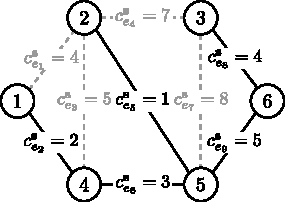
\includegraphics[width=\textwidth]{Chapter_II/INC-MST-example/a}
		\caption{}
		\label{fig:increxample:a}
	\end{subfigure}
	\hfill
	\begin{subfigure}[b]{0.3\textwidth}
		\includegraphics[width=\textwidth]{Chapter_II/INC-MST-example/b}
		\caption{}
		\label{fig:increxample:b}
	\end{subfigure}
	\hfill
	\begin{subfigure}[b]{0.3\textwidth}
		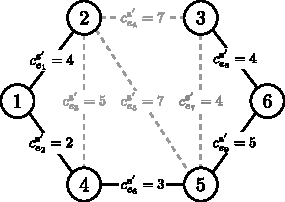
\includegraphics[width=\textwidth]{Chapter_II/INC-MST-example/c}
		\caption{}
		\label{fig:increxample:c}
	\end{subfigure}
	\hfill\null
	\caption{
		Różnice między rozwiązaniami problemów \textsc{Minimum Spanning Tree} i~\textsc{Incremental MST} z~parametrem $k = 1$.
		\textbf{(a)}~Optymalne rozwiązanie problemu minimalnego drzewa rozpinającego $T^{\ast}_{\textbf{s}}$ dla scenariusza $\textbf{s} = \left\{ 4, 2, 5, 7, 1, 3, 8, 4, 5 \right\}$ o~całkowitym koszcie rozwiązania $v_{\textsc{MST}} \left( T^{\ast}_{\textbf{s}}, \textbf{s} \right) = 15$.	
		\textbf{(b)}~Niedopuszczalne rozwiązanie $T^{\ast}_{\textbf{s}^{\prime}} = \left\{ e_{1}, e_{2}, e_{6}, e_{7}, e_{8} \right\}$ problemu \textsc{Incremental Minimum Spanning Tree}, będące jednocześnie optymalnym dla scenariusza $\textbf{s}^{\prime}$ w~problemie \textsc{MST} o~koszcie $v_{\textsc{MST}} \left( T^{\ast}_{\textbf{s}^{\prime}}, \textbf{s}^{\prime} \right) = 17$.
		\textbf{(c)}~Optymalne rozwiązanie problemu \textsc{Incremental MST} i~scenariusza $\textbf{s}^{\prime}$: $T^{\ast} = \left\{ e_{1}, e_{2}, e_{6}, e_{8}, e_{9} \right\}$ o~całkowitym koszcie $v^{\ast}_{\textbf{s}^{\prime}} = 18$.
	}
	\label{fig:increxample}
\end{figure}

Niestety wraz ze wzrostem grafu (oraz przede wszystkim parametru $k$) rozwiązanie to staje się nieefektywne~--- jak mogliśmy zauważyć, opisany algorytm działa sekwencyjnie, co każdą iterację zmniejszając wartość funkcji $f \left( T^{i}, T \right)$, gdzie $T^{i}$ to rozwiązanie uzyskane podczas $i$-tej iteracji.
Ogólnie: $f \left( T^{i-1}, T \right) - 1 = f \left( T^{i}, T \right)$\footnote{
	W rozdziale \ref{ch:binaryIncMST} omówimy algorytm, który także działa iteracyjnie ze względu na wartość tej funkcji, lecz przedstawiona własność nie jest zachowana, co przekłada się na dużo lepsze otrzymywane czasy działania.
}.
Naszym zadaniem zatem jest konstrukcja takiego ciągu drzew rozpinających $T^{1}, \dots, T^{l}$, aby $f \left( T^{l}, T^{0} \right) = k$, gdzie $T^{0} = T$ i~jest początkowym rozwiązaniem problemu $\mathcal{P}$ dla pierwotnego scenariusza, zaś $l = f \left( T^{1}, T^{0} \right) - k + 1$ ($k = f \left( T^{l}, T^{0} \right) = f \left( T^{l-1}, T^{0} \right) - 1 = \dots =  f \left( T^{2}, T^{0} \right) - \left( l - 2 \right) = f \left( T^{1}, T^{0} \right) - \left( l - 1 \right) = k$~--- ogólnie $f \left( T^{l - i}, T^{0} \right) - i = k$).
Każde kolejne rozwiązanie powinno zatem składać się z~coraz to większej liczby krawędzi należących do $T^{0}$.
Aby to osiągnąć, dla każdej $i$-tej iteracji musielibyśmy rozpatrzyć wszystkie możliwe podziały drzewa $T^{i-1}$, powstałe w~wyniku usunięcia jednej z~krawędzi $e^{i-1} \in T^{i-1} \setminus T^{0}$~--- innymi słowy wszystkie takie pary drzew $\left( T^{i-1}_{1}, T^{i-1}_{2} \right)$, których łączna liczba krawędzi nie należących do drzewa $T^{0}$ jest o~$1$ mniejsza niż dla drzewa $T^{i-1}$. 
Takich par w~$i$--tej iteracji jest dokładnie $f \left( T^{1}, T^{0} \right) - k - \left( i - 1 \right)$ (iteracje numerujemy rozpoczynając od $i = 1$).
Dla każdej takiej pary musimy następnie znaleźć wszystkie krawędzie należące do zbioru $\mathcal{Q} \left( T^{i-1}, e^{i-1} \right) \cap T^{0}$, łączące ze sobą dane poddrzewa\footnote{
	O zbiorze krawędzi łączącym dwa poddrzewa rozpinające, które powstały w~wyniku cięcia oryginalnego drzewa, pisaliśmy w~poprzednim rozdziale (\ref{sec:mst}).
}, gdzie krawędź $e^{i-1} \in T^{i-1}$ jest krawędzią usuwaną z~$T^{i-1}$, nienależącą do $T^{0}$.
Na samym końcu musimy stworzyć nowe drzewo, do którego dołączymy krawędź $e^{\prime} \in \mathcal{Q} \left( T^{i-1}, e^{i-1} \right) \cap T^{0}$ o~najkorzystniejszym stosunku jej wagi do kosztu usuniętej krawędzi.
Formalnie: $T^{i} = \left( \left\{ e : e \in T^{i-1} \right\} \setminus e^{i-1} \right) \cup e^{\prime} \; : \; e^{\prime} = \min arg_{e^{\prime}} \frac{c_{e^{\prime}}}{c_{e^{i-1}}}$. 

Złożoność takiego rozwiązania to $O \left( \left| V \right| \cdot \left(l^{3} + \left| V \right| \right) \right)$, gdzie $l$ to liczba iteracji algorytmu (miara tego, jak daleko od dopuszczalności dla \textsc{Incremental MST} jest optymalne rozwiązanie dla problemu \textsc{MST}).
W~pierwszej iteracji liczba potencjalnych krawędzi do usunięcia wynosi $l - 1$ i~stopniowo maleje.
Dla każdej takiej krawędzi musimy zaś zdeterminować zbiór możliwych do dodania łuków.
Bez straty ogólności możemy założyć, że po uzyskaniu podziału drzewa $T^{i-1}$ na $\left( T^{i-1}_{1}, T^{i-1}_{2} \right)$, aby ustalić właściwy zbiór krawędzi, będziemy szukać odpowiednich łuków wychodzących z~wierzchołków, należących do drzewa o~mniejszej ich liczbie (będziemy analizować krawędzie wychodzące z~wierzchołków $v \in T^{i-1}_{1}$, jeśli $\left| \left\{ v_{i} : e_{ij} \in T^{i-1}_{1} \right\} \right| \leqslant \left| \left\{ v_{i} : e_{ij} \in T^{i-1}_{2} \right\} \right|$\footnote{
	Wyrażenie $\left| \left\{ v_{i} : e_{ij} \in T \right\} \right|$ oznacza po prostu liczbę wierzchołków, które łączą ze sobą krawędzie należące do drzewa $T$~--- jako że rozpatrujemy tylko grafy nieskierowane, $\left\{ v_{i} : e_{ij} \in T \right\} \equiv \left\{ v_{j} : e_{ij} \in T \right\}$ (kolejność wierzchołków w~zbiorach nie jest istotna).
}, bądź z~$v \in T^{i-1}_{2}$ w~przeciwnym przypadku).
Możemy założyć, że w~najgorszym z~możliwych przypadków wszystkie krawędzie, tworzące podział na poddrzewa $T^{i-1}_{1}$ oraz $T^{i-1}_{2}$, dzielą oryginalne drzewo $T^{i-1}$ na możliwie równe części~--- każdorazowe ustalenie zbioru krawędzi $\mathcal{Q} \left( T^{i-1}, e^{i-1} \right)$ (a tym samym $\mathcal{Q} \left( T^{i-1}, e^{i-1} \right) \cap T^{0}$) zatem wymagać będzie od nas przeglądnięcia wszystkich krawędzi wychodzących z~$\frac{\left| V \right| - 1}{2} - \frac{i - j}{2}$ wierzchołków, gdzie $j$ to indeks krawędzi $e_{j}$, według której dokonujemy podziału.
Możemy także założyć, że w~pesymistycznym przypadku będziemy mieli do czynienia z~grafem pełnym, gdzie stopnień każdego wierzchołka $v \in V$ wynosi $d \left( v \right) = \left| V \right| - 1$.
Stąd otrzymujemy wzór na ogólną liczbę porównań wybranych par krawędzi $\left( e^{i-1}, e^{\prime} \right)$, gdzie $e^{i-1}$ jest krawędzią wychodzącą z~rozwiązania, zaś $e^{\prime}$~--- wchodzącą:

\begin{gather*}
	\sum_{\mathclap{i=1}}^{\mathclap{l-1}} \sum_{\mathclap{j=1}}^{\mathclap{i}} \left( \left| V \right| - 1 \right) \cdot \left( \frac{\left| V \right| - 1}{2} - \frac{i - j}{2} \right) = \frac{1}{12} \cdot \left( l - 3 \right) \cdot \left( \left| V \right| - 1 \right) \cdot \left( l^{2} - 3 \cdot l \cdot \left| V \right| + 2 \right) = \\ 
	= \frac{l^{3} \cdot \left( \left| V \right| - 1 \right)}{12} - \frac{l^{2} \cdot \left( \left| V \right|^{2} - 1 \right)}{4} + \frac{3 \cdot l \cdot \left| V \right|^{2}}{4} - \frac{7 \cdot l \cdot \left| V \right|}{12} - \frac{l}{6} - \frac{\left| V \right|}{2} + \frac{1}{2}\text{.}
\end{gather*}

Dodając do tego koszt odnalezienia potencjalnych krawędzi, które będziemy usuwać ($\left| V \right| - 1$~--- wystarczy raz przejść po wszystkich krawędziach drzewa $T^{0}$; z~każdą następną iteracją zbiór ten pomniejsza się o~ustaloną krawędź, więc nie musimy za każdym razem rozpoczynać analizy krawędzi drzewa od nowa), otrzymujemy~--- wymieniony na samym początku~--- stopień złożoności, który ilustruje wykres \ref{fig:incmst3D}.

\begin{figure}[!htbp]
	\renewcommand\figurename{Wykres}
	\null\hfill
	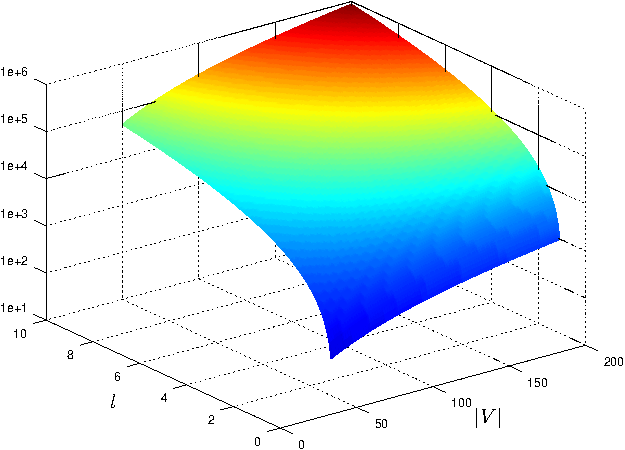
\includegraphics[width=0.65\textwidth]{Chapter_II/INC-MST-Other/incmst3DPlot_psfrag}
	\hfill\null
	\caption{
		Stopień złożoności naiwnego algorytmu rozwiązującego problem minimalnego drzewa rozpinającego w~wersji \textsc{Incremental} głównie zależy od liczby krawędzi, o~które optymalne rozwiązanie dla problemu \textsc{MST} różni się od dopuszczalnej liczby nowych krawędzi względem starego rozwiązania w~problemie \textsc{Incremental Minimum Spanning Tree}.
	}
	\label{fig:incmst3D}
\end{figure}

Najprostszym z~możliwych opisów tak zdefiniowanego problemu jest model przedstawiony w~\ref{mod:lpmodel1} dla nowego scenariusza $\textbf{s}^{\prime}$, gdzie $T_{0}$ oznacza nasze drzewo początkowe, $T^{\ast}$~--- optymalne rozwiązanie dla problemu \textsc{IMST}, gdzie $x_{e} = 1$ oznacza należenie do niego krawędzi $e \in E$. 

\newpage

\begin{subequations}
	\begin{alignat}{5}
	v^{\textsc{IMST}} \left( T^{\ast}, \textbf{s}^{\prime} \right) \; = \; & \text{min} & & \sum_{\mathclap{e \in E}} c^{\textbf{s}^{\prime}}_{e} \cdot x_{e}\text{,} \quad\quad &\\
	& & \quad & x_{e} = 1\text{,} & & \forall e \in T_{0}\text{,} & \quad\quad &\\
	& & & \sum_{\mathclap{e \in T^{\ast} \setminus T_{0}}} x_{e} \leqslant k \text{,} & & & \quad\quad &\\
	& & & \phantom{\sum} x_{e} \in \left\{ 0, 1 \right\}\text{,} && \forall e \in E\text{.} && \quad\quad &
	\end{alignat}\label{mod:lpmodel1}
\end{subequations}



\subsection{Zagadnienia oparte na problemie INCREMENTAL}



\subsubsection{Problem adwersarza}\label{sec:adv}


Przyjrzymy się teraz nieco bardziej rozbudowanemu problemowi, znanego jako \textbf{problem adwersarza} (ang. adversarial problem).
W~tym przypadku zamiast skupiać się na minimalizacji rozwiązania, naszym celem (celem adwersarza) jest maksymalizowanie jego wartości~\cite[$2$]{DBLP:journals/corr/NasrabadiO13}.
Osiągnąć cel możemy poprzez wybór takiego scenariusza, dla którego najlepsza wartość rozwiązania problemu \textsc{Incremental} będzie najgorsza:

\begin{equation}
	\max_{\mathclap{\textbf{s}^{\prime} \in S}} \min_{\mathclap{\textbf{y} \in X^{k}_{\textbf{x}}}} v \left( \textbf{y}, \textbf{s}^{\prime} \right)\text{.}
\end{equation}

Łatwo zauważyć, że oba te wybory~--- adwersarza i~osoby wybierającej rozwiązanie dla problemu \textsc{Incremental}~--- nie zależą od siebie, przez co problem sprowadza się do omawianego wcześniej, z~tą różnicą, że zamiast posiadania dwóch scenariuszy (gdzie na podstawie pierwszego wybieraliśmy rozwiązanie w~postaci wektora $\textbf{x}$), mamy ich większą liczbę i~adwersarz dla każdego z~nich musi policzyć wartość $\min_{\textbf{y} \in X^{k}_{\textbf{x}}} v \left( \textbf{y}, \textbf{s}^{\prime} \right)$, by móc wybrać najbardziej sprzyjający mu scenariusz (skutkujący zwróceniem jak największej wartości).
Problem można zatem bez trudu zrównoleglić (rozwiązywać jednocześnie klasyczny problem \textsc{IMST} dla wielu scenariuszy naraz), przez co nie da się o~nim napisać wiele więcej ponad to, co już napisaliśmy przy omawianiu wcześniejszego problemu.


\subsubsection{Odporny problem przyrostowy z~możliwością poprawy rozwiązania}\label{sub:rrimst}


Kolejnym rozszerzeniem poprzednio omawianego problemu jest problem \textbf{odpornej optymalizacji przyrostowej} (ang. \textit{robust incremental optimization}~\cite[$2$]{DBLP:journals/corr/NasrabadiO13}).
W~odróżnieniu od problemów typu \textsc{Incremental} oraz problemu adwersarza, w~tym przypadku chcemy cofnąć się o~jeden krok w~procesie poszukiwania rozwiązania i~zminimalizować jego wartość, uwzględniając dodatkowo naszą pierwszą decyzję~--- tą odnoszącą się do wektora $\textbf{x}$, będącą podstawą do rozwiązania problemu \textsc{Incremental}.
Jak możemy się domyślać, problem ten definiujemy w~następujący sposób:

\begin{equation}\label{eq:rimstdef}
	\min_{\mathclap{\textbf{x} \in X}} \left( v \left( \textbf{x}, \textbf{s} \right) + \max_{\mathclap{\textbf{s}^{\prime} \in S}} \min_{\mathclap{\textbf{y} \in X^{k}_{\textbf{x}}}} v \left( \textbf{y}, \textbf{s}^{\prime} \right) \right)\text{.}
\end{equation}

Niech początkowym scenariuszem, na podstawie którego wybierzemy wektor $\textbf{x}$, będzie $\textbf{s}_{0} = \left\{ 1, 1, 1, 1, 1, 1 \right\}$, zaś scenariuszami, spośród których będzie mógł wybierać adwersarz:

\begin{itemize}
	\item $\textbf{s}_{1} = \left\{ 4, 6, 1, 9, 3, 7 \right\}$ oraz
	\item $\textbf{s}_{2} = \left\{ 7, 3, 9, 1, 9, 4 \right\}$.
\end{itemize}

Oczywiście wybór scenariusza $\textbf{s}_{0}$ nie jest przypadkowy~--- naszym celem jest pokazanie możliwej do osiągnięcia różnicy w~jakości rozwiązania dla dwóch różnych sposobów podejścia do zadanego problemu: klasycznego, polegającego na prostym wybraniu rozwiązania o~najmniejszym koszcie w~pierwszym kroku, z~pominięciem problemu adwersarza, tożsamym z~rozwiązaniem zagadnienia minimalnego drzewa rozpinającego dla pojedynczego scenariusza ($\min_{\textbf{x} \in X} v \left( \textbf{x}, \textbf{s} \right)$), oraz odpornego. 
Łatwo zauważyć, że w~przypadku tak dobranych scenariuszy (tak jak to pokazano na rysunkach od \ref{fig:robincrexample:a} do \ref{fig:robincrexample:f} oraz \ref{fig:robincrexampleopt}), na pozór nic nie znacząca decyzja o~pierwszym wyborze rozwiązania (jako że wszystkie koszty w~scenariuszu $\textbf{s}_{0}$ są sobie równe, dowolnie wybrane drzewo rozpinające charakteryzuje ten sam koszt~--- będzie zatem wyborem optymalnym), w~przypadku pojawienia się odpowiednich zmian kosztów, może zaważyć na optymalności całego rozwiązania w~myśl \ref{eq:rimstdef}.
Dodatkowo niech parametr dla problemu \textsc{Incremental Minimum Spanning Tree} wynosi $k = 1$.
Przedstawiany na rysunkach \ref{fig:robincrexample:a}--\ref{fig:robincrexample:f}, \ref{fig:robincrexampleopt} graf jest na tyle nieduży, że z~powodzeniem możemy rozwiązać ten problem, wykorzystując do tego pełen przegląd wszystkich możliwych rozwiązań (ang. \textit{brute force})~--- dla każdego możliwego drzewa rozpinającego, reprezentowanego przez wektor $\textbf{x}$, możemy wyliczyć wartość $v \left( \textbf{x}, \textbf{s} \right) + \max_{\textbf{s}^{\prime} \in S} \min_{\textbf{y} \in X^{k}_{\textbf{x}}} v \left( \textbf{y}, \textbf{s}^{\prime} \right)$, rozwiązując po drodze $24$ egzemplarze problemu \textsc{Incremental Minimum Spanning Tree} (po dwa dla każdej z~$12$ instancji problemu \textsc{Adversarial Incremental Minimum Spanning Tree}~--- $X = \left\{ \textbf{x}_{1}, \textbf{x}_{1}, \dots, \textbf{x}_{12} \right\}$).
Otrzymane wyniki zgromadzono w~tabeli \ref{tab:minmaxrobexample}, która reprezentuje wartości optymalnych rozwiązań poszczególnych składowych głównego problemu.
Tabela nie przedstawia natomiast wyników, uzyskanych dla problemu przedstawionego w~równaniu (\ref{eq:rimstdef})~--- możemy dostrzec, że dla tak specyficznie zdefiniowanego scenariusza $\textbf{s}_{0}$, suma kosztów wszystkich krawędzi w~dowolnie wybranym drzewie rozpinającym jest taka sama (wynosi $4$), więc wartości te możemy z~powodzeniem obliczyć sami (dodając tą wartość do przedstawionych wyników dla problemu adwersarza)\footnote{
	Ze względu na dość ogólne znaczenie, jakie ma zwrot odpornej optymalizacji przyrostowej, będziemy chcieli od niego uciec i~od tej pory odnosić się do naszego problemu, u~którego podstaw leży problem minimalnego drzewa rozpinającego w~wersji \textsc{Incremental}, jako do problemu \textsc{Recoverable Robust Incremental Minimum Spanning Tree} (dalej \textsc{RRIMST}), gdzie takie oznaczenie bezpośrednio wskazuje na podstawowy problem, z~jakim się będziemy zmagać.
	W~literaturze często możemy się dodatkowo spotkać z~inną jego nazwą: \textsc{k-Dist Recoverable Robust Spanning Tree}~\cite{Kasperski2014}.
}.

\begin{table}[!htbp]
	\caption{
		Tabela przedstawiająca wszystkie, możliwe do skonstruowania dla grafu prezentowanego na rysunkach od \ref{fig:robincrexample:a} do \ref{fig:robincrexample:f} oraz \ref{fig:robincrexampleopt}, drzewa rozpinające, reprezentowane przez wektory od $\textbf{x}_{1}$ do $\textbf{x}_{12}$, wartości optymalnych rozwiązań problemów \textsc{Incremental Minimum Spanning Tree} dla wszystkich scenariuszy adwersarza ($\textbf{s}_{1}$ oraz $\textbf{s}_{2}$) z~uwzględnieniem parametru $k = 1$ oraz (w ostatniej kolumnie) wartość optymalnego rozwiązania problemu adwersarza dla zbioru jego scenariuszy oraz danego wektora początkowego $\textbf{x}$.
		Rozwiązania, reprezentowane przez wektory od $\textbf{x}_{1}$ do $\textbf{x}_{12}$, są posortowane według rosnącej wartości dla odpowiadającego im rozwiązania problemu \textsc{Adversarial Incremental Minimum Spanning Tree}.
	}
	\label{tab:minmaxrobexample}
	\begin{tabular}{cccccccccc}
		\cline{8-10}
		\multicolumn{2}{l}{}       &         &         &         &         &         & \multicolumn{3}{c}{Scenariusze}                                                                                                                                                                                              \\
		$X$              & $e_{1}$ & $e_{2}$ & $e_{3}$ & $e_{4}$ & $e_{5}$ & $e_{6}$ & 	\footnotesize$v^{\textsc{IMST}}_{\textbf{s}_{1}} = \min_{\textbf{y} \in X^{k}_{\textbf{x}}} v \left( \textbf{y}, \textbf{s}_{1} \right) $ &\footnotesize $v^{\textsc{IMST}}_{\textbf{s}_{2}} = \min_{\textbf{y} \in X^{k}_{\textbf{x}}} v \left( \textbf{y}, \textbf{s}_{2} \right)$ &\footnotesize $\max \left\{ v^{\textsc{IMST}}_{\textbf{s}_{1}}, v^{\textsc{IMST}}_{\textbf{s}_{2}} \right\} $ \\\normalsize
		$\textbf{x}_{1}$	&	$1$	&	$1$	&	$0$	&	$1$	&	$1$	&	$0$	&	$14$	&	$15$	&	$15$	\\
		$\textbf{x}_{2}$	&	$1$	&	$0$	&	$0$	&	$1$	&	$1$	&	$1$	&	$15$	&	$15$	&	$15$	\\
		$\textbf{x}_{3}$	&	$0$	&	$1$	&	$0$	&	$1$	&	$1$	&	$1$	&	$17$	&	$15$	&	$17$	\\
		$\textbf{x}_{4}$	&	$0$	&	$1$	&	$1$	&	$0$	&	$1$	&	$1$	&	$14$	&	$17$	&	$17$	\\
		$\textbf{x}_{5}$	&	$1$	&	$0$	&	$1$	&	$1$	&	$0$	&	$1$	&	$15$	&	$15$	&	$15$	\\
		$\textbf{x}_{6}$	&	$0$	&	$1$	&	$1$	&	$1$	&	$0$	&	$1$	&	$17$	&	$15$	&	$17$	\\
		$\textbf{x}_{7}$	&	$1$	&	$1$	&	$1$	&	$0$	&	$0$	&	$1$	&	$14$	&	$15$	&	$15$	\\
		$\textbf{x}_{8}$	&	$1$	&	$0$	&	$1$	&	$0$	&	$1$	&	$1$	&	$14$	&	$21$	&	$21$	\\
		$\textbf{x}_{9}$	&	$1$	&	$0$	&	$1$	&	$1$	&	$1$	&	$0$	&	$14$	&	$20$	&	$20$	\\
		$\textbf{x}_{10}$	&	$0$	&	$1$	&	$1$	&	$1$	&	$1$	&	$0$	&	$14$	&	$17$	&	$17$	\\
		$\textbf{x}_{11}$	&	$1$	&	$1$	&	$1$	&	$0$	&	$1$	&	$0$	&	$14$	&	$20$	&	$20$	\\
		$\textbf{x}_{12}$	&	$1$	&	$1$	&	$0$	&	$1$	&	$0$	&	$1$	&	$18$	&	$15$	&	$18$	\\
		\hline
	\end{tabular}
\end{table}

\begin{figure}[!htbp]
	\null\hfill
	\begin{subfigure}[b]{0.3\textwidth}
		\includegraphics[width=\textwidth]{Chapter_II/ROB-INC-MST-example/a1}
		\caption{}
		\label{fig:robincrexample:a}
	\end{subfigure}
	\hfill
	\begin{subfigure}[b]{0.3\textwidth}
		\includegraphics[width=\textwidth]{Chapter_II/ROB-INC-MST-example/b1}
		\caption{}
		\label{fig:robincrexample:b}
	\end{subfigure}
	\hfill
	\begin{subfigure}[b]{0.3\textwidth}
		\includegraphics[width=\textwidth]{Chapter_II/ROB-INC-MST-example/c1}
		\caption{}
		\label{fig:robincrexample:c}
	\end{subfigure}
	\hfill\null
	\caption{
		Sytuacja dla problemu \textsc{Recoverable Robust Incremental Minimum Spanning Tree} dla wybranego rozwiązania $T = T_{\textbf{x}_{5}} = \left\{ e_{1}, e_{3}, e_{4}, e_{6} \right\}$, gdzie dwa ostatnie rysunki prezentują drzewa, z~których rozwiązanie wybierać będzie adwersarz.
		\textbf{(a)}~Drzewo rozpinające wybrane przez podejmującego decyzję (nie przez adwersarza), reprezentowane przez wektor $\textbf{x}_{5} = \left[ 1, 0, 1, 1, 0, 1 \right]$ (patrz: tabela \ref{tab:minmaxrobexample}) o~sumie kosztów wybranych krawędzi $v \left( T, \textbf{s}_{0} \right) = 4$.
		\textbf{(b)}~Minimalne drzewo rozpinające $T^{\textsc{IMST}}_{\textbf{s}_{1}}$ o~najmniejszym koszcie dla problemu typu \textsc{Incremental} z~parametrem $k = 1$ oraz drzewem początkowym $T$.
		Krawędzią, która weszła do rozwiązania nowego drzewa, jest $e_{5}$ ($T^{\textsc{IMST}}_{\textbf{s}_{1}} \setminus T = \left\{ e_{5} \right\}$), zaś usuniętą~--- $e_{4}$.
		Koszt rozwiązania wynosi $15$.
		\textbf{(c)}~Rozwiązanie problemu \textsc{Incremental Minimum Spanning Tree} dla drugiego scenariusza ($\textbf{s}_{2}$) i~tego samego początkowego drzewa rozpinającego $T$.
		Liczba krawędzi nie należących do drzewa $T$, jednocześnie zawierających się w~nowym rozwiązaniu $T^{\textsc{IMST}}_{\textbf{s}_{2}}$, wynosi $1$.
		W~obu przypadkach koszt optymalnych rozwiązań danego problemu jest taki sam ($v \left(  T^{\textsc{IMST}}_{\textbf{s}_{1}}, \textbf{s}_{1} \right) = v \left(  T^{\textsc{IMST}}_{\textbf{s}_{2}}, \textbf{s}_{2} \right) = 15$), toteż wybór scenariusza ($\textbf{s}_{1}$ lub $\textbf{s}_{2}$), który zostanie podjęty przez adwersarza, nie ma żadnego znaczenia (dla rozwiązania reprezentowanego przez $\textbf{x}_{5}$).
	}
\end{figure}

\begin{figure}[!htbp]
	\null\hfill
	\ContinuedFloat
	\begin{subfigure}[b]{0.3\textwidth}
		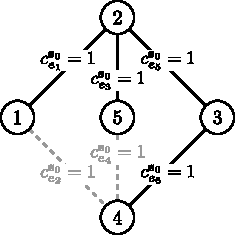
\includegraphics[width=\textwidth]{Chapter_II/ROB-INC-MST-example/a2}
		\caption{}
		\label{fig:robincrexample:d}
	\end{subfigure}
	\hfill
	\begin{subfigure}[b]{0.3\textwidth}
		\includegraphics[width=\textwidth]{Chapter_II/ROB-INC-MST-example/b2}
		\caption{}
		\label{fig:robincrexample:e}
	\end{subfigure}
	\hfill
	\begin{subfigure}[b]{0.3\textwidth}
		\includegraphics[width=\textwidth]{Chapter_II/ROB-INC-MST-example/c2}
		\caption{}
		\label{fig:robincrexample:f}
	\end{subfigure}
	\hfill\null
	\caption{
		Wybrane drzewo rozpinające $T_{\textbf{x}_{8}}$ (patrz: tabela \ref{tab:minmaxrobexample}) dla problemu \textsc{Recoverable Robust Incremental Minimum Spanning Tree} wraz z~dwoma drzewami, będącymi optymalnymi rozwiązaniami problemu \textsc{Incremental Minimum Spanning Tree} odpowiednio dla scenariuszy $\textbf{s}_{1}$ oraz $\textbf{s}_{2}$.
		\textbf{(d)}~Wybrane rozwiązanie, reprezentowane przez wektor $\textbf{x}_{8} = \left[ 1, 0, 1, 0, 1, 1 \right]$, o~koszcie $4$.
		\textbf{(e)}~Optymalne rozwiązanie problemu minimalnego drzewa rozpinającego w~wersji \textsc{Incremental} dla scenariusza $\textbf{s}_{1}$ (początkowego $\textbf{s}_{0}$) o~wartości rozwiązania równej $14$.
		\textbf{(f)}~Minimalne drzewo rozpinające, które jest optymalnym rozwiązaniem dla tego samego problemu, dla scenariusza $\textbf{s}_{2}$.
		Jako że koszt tego rozwiązania jest największy spośród wszystkich rozwiązań problemu \textsc{IMST} dla scenariuszy adwersarza (koszt tego rozwiązania wynosi $21$), zostanie ono przez niego wybrane.
		Poprzednie rozwiązanie (o koszcie $14$) zostanie odrzucone jako nieopłacalne.
	}
	\label{fig:robincrexample}
\end{figure}

\begin{figure}[!h]
	\null\hfill
	\begin{subfigure}[b]{0.3\textwidth}
		\includegraphics[width=\textwidth]{Chapter_II/ROB-INC-MST-example/d1}
		\caption{}
		\label{fig:robincrexampleopt:a}
	\end{subfigure}
	\hfill
	\begin{subfigure}[b]{0.3\textwidth}
		\includegraphics[width=\textwidth]{Chapter_II/ROB-INC-MST-example/d2}
		\caption{}
		\label{fig:robincrexampleopt:b}
	\end{subfigure}
	\hfill\null
	\caption{
		Optymalne rozwiązania problemów \textsc{Incremental Minimum Spanning Tree} dla podwyższonej wartości parametru $k = 2$, która dla prezentowanego grafu jest wystarczająca, aby zwracane rozwiązania dla poszczególnych scenariuszy były takie same jak dla klasycznego problemu minimalnego drzewa rozpinającego.
		\textbf{(a)}~Minimalne drzewo rozpinające dla scenariusza $\textbf{s}_{1} = \left[ 4, 6, 1, 9, 3, 7 \right]$.
		\textbf{(b)}~Optymalne rozwiązanie problemu minimalnego drzewa rozpinającego w~wersji \textsc{Incremental} dla scenariusza $\textbf{s}_{2}$.
	}
	\label{fig:robincrexampleopt}
\end{figure}

Widzimy zatem jak bardzo skomplikowanym i~trudnym obliczeniowo procesem jest generowanie rozwiązań dla problemu \textsc{Recoverable Robust Incremental Minimum Spanning Tree} i~jak ciężko musieliśmy pracować, aby dojść do tego punktu (po drodze poznaliśmy dwa inne problemy, które są tylko jego częścią).
Poziom złożoności opisanego przez nas problemu dodatkowo potęguje fakt, że przedstawiony przez nas przykład tyczył się grafu o~bardzo niewielkich rozmiarach~--- liczył on sobie zaledwie $6$ krawędzi i~$5$ wierzchołków.
Jego konstrukcja z~kolei w~bardzo znaczący sposób ograniczyła liczbę możliwych rozwiązań (liczebność zbioru $X$), my zaś jeszcze bardziej uprościliśmy problem, wybierając do problemu adwersarza najmniejszą liczbę scenariuszy, jaka ma jeszcze dla tego problemu sens ($\textbf{s}_{1}$, $\textbf{s}_{2}$).
W ogólnym przypadku nie możemy mieć nadziei, że takie podejście do problemu (rozwiązanie siłowe) będzie możliwe.




\section{Podsumowanie rozdziału}




Widzimy, że sposobów podejścia do problemów optymalizacyjnych jest bardzo dużo, zaś te przez nas przedstawione stanowią już dużo bardziej zaawansowane spojrzenie na ten problem, niż pokazaliśmy w~poprzednim rozdziale, omawiając podstawowe pojęcia związanie z~problemem minimalnego drzewa rozpinającego.
Wraz z~omawianiem kolejnych zagadnień w~tym rozdziale mogliśmy zauważyć naszą potrzebę konstrukcji takich rozwiązań, które nie tylko pozwalać nam będą wybierać najlepsze dla nas rozwiązania, gdy zawczasu przewidzimy wszystkie możliwe sytuacje (im większy zbiór zdarzeń zostanie przez nas uwzględniony, tym bardziej ogólne rozwiązanie najprawdopodobniej wybierzemy), ale i~na bieżąco będą reagować na zaistniałe sytuacje (co pozwala na wybór znacznie lepszych rozwiązań, uwzględniających tylko najbliższą przyszłość).
Dodatkowo chcieliśmy, aby tak konstruowane rozwiązania łatwo poddawały się zmianom~--- aby wybór jednego (optymalnego w~czasie jego wyboru) nie powodował konieczności jego całkowitej rekonstrukcji w~przypadku zajścia przewidzianego przez nas scenariusza.
W~związku z~tym podaliśmy formułę, która wybiera dla nas takie rozwiązania, które nie tylko łatwo modyfikować (poprawiać), ale i~takie, które zapewniają najlepsze rezultaty w~najbliższej, przewidzianej przez nas, przyszłości.
Niestety wraz z~rosnącymi oczekiwaniami oczywiście rósł poziom skomplikowania opisywanych problemów i~dla ostatniego z~nich (\textsc{Recoverable Robust Incremental Minimum Spanning Tree} z~dyskretnym zbiorem scenariuszy $S$) zwyczajnie nie jesteśmy już w~stanie podać wielomianowego algorytmu, który radziłby sobie z~danym problemem (w przypadku dwóch pozostałych~--- \textsc{Adversarial Incremental Minimum Spanning Tree} oraz \textsc{Incremental Minimum Spanning Tree}~--- podamy je w~następnych rozdziałach).
W~związku z~tym, w~rozdziale \ref{ch:localSearch} przedstawimy inną metodę podejścia do danego problemu (heurystyczną).
Dodatkowo warto w~tym miejscu podkreślić, że wszystkie do tej pory omówione przypadki problemów koncentrowały się na znanej, ograniczonej przez daną stałą, liczbie scenariuszy (z góry ustalonym, dyskretnym ich zbiorze $S$), co zdecydowanie upraszcza sposób patrzenia się na te problemy~--- analizę przez nas omawianych przypadków (tyle że dla nieograniczonej liczby scenariuszy, gdzie ich liczba jest częścią danych wejściowych dla problemu) możemy znaleźć w~\cite{DBLP:journals/ipl/KasperskiZ09}.
Następnym rozdziałem odejdziemy nieco od omawianych jak dotąd problemów~--- wyjaśnimy znaczenie modelu (równania \ref{mod:lpmodel1}), przedstawiając podstawowe pojęcia z~nieco innego obszaru algorytmiki~--- programowania \textsc{LP}, \textsc{MIP} oraz \text{IP}.
	\clearpage
	
	\clearpage
	\chapter{Problemy programowania liniowego}\label{ch:linearprog}
\thispagestyle{chapterBeginStyle}





Chcąc podjąć próbę formalnego opisania przedstawionych wcześniej problemów, należy najpierw zapoznać się z~ogólnymi zasadami ich zapisywania.
Jak mogliśmy zaobserwować w~poprzednim rozdziale, opisując problem typu \textsc{Incremental}, uciekliśmy się do przedstawienia go za pomocą serii nierówności oraz równości (\ref{mod:lpmodel1})~--- innymi słowy zapisaliśmy go w~postaci \textbf{modelu programowania liniowego}.
Możliwość przekształcenia dowolnie zadanego problemu do takiej postaci może nam zagwarantować odnalezienie jego istniejącego rozwiązania w~czasie wielomianowym i~takie narzędzie może stanowić doskonały punkt wyjściowy do dalszych rozważań.
W tym rozdziale omówimy ten sposób podejścia do problemów oraz przedstawimy narzędzia, które posłużą nam do konstrukcji algorytmu, rozwiązującego problem odpornej optymalizacji dla wyszukiwania minimalnego drzewa rozpinającego w~wersji \textsc{Incremental}, w rozdziale następnym.
Po drodze przedstawimy także alternatywne sposoby na radzenie sobie z problemami \textsc{MST} oraz \textsc{IMST}.




\section{Programowanie liniowe}




Mając na uwadze, że nie chcemy zajmować się zagadnieniem programowania liniowego samym w~sobie, gdyż nie jest to naszym celem, w~poniższym rozdziale zostaną przytoczone tylko podstawowe fakty, niezbędne do zrozumienia dalszej jego części.
Punktem wyjścia do pozyskania głębszej wiedzy na poruszany w~tym rozdziale temat może być książka~\cite{Papadimitriou:1982:COA:31027}, która omawia wszystkie aspekty tej dziedziny, począwszy od programowania wklęsłego, przez liniowe, do całkowitoliczbowego, tłumacząc zasady działania każdego z~tych modeli.

Przez pojęcie \textbf{programowania liniowego} będziemy rozumieli zbiór liniowych równań oraz nierówności wraz z~określoną dla nich \textbf{funkcją celu}, która także musi przybrać formę liniowego wyrażenia arytmetycznego.
Zbiór tych ograniczeń wraz z~funkcją celu będziemy nazywali \textbf{modelem prymalnym}\footnote{
	Terminem ,,prymalny'' będziemy określać modele programowania liniowego/całkowitoliczbowego, których funkcja celu jest minimalizacyjna.
	Problemem \textbf{dualnym} nazwiemy model, który skupia się na maksymalizowaniu jej wartości.
	Zagadnienia związane z~obydwoma modelami zostały dokładniej opisane w~książce~\cite[$67$--$73$]{Papadimitriou:1982:COA:31027}.
} programowania liniowego.
Schemat takiego modelu wygląda następująco:

\begin{subequations}
	\begin{alignat}{4}
	& \text{min} & & f \left( \textbf{x}, \dots \right)\textrm{,} &&& \\
	& \text{takie, że} & \quad & g_{1} \left( \textbf{x}, \dots \right) \quad \Diamond_{1} \quad b_{1}\textrm{,} && \text{(ang. \textit{subject to})}&\label{eq:lp:b} \\
	& & & g_{2} \left( \textbf{x}, \dots \right) \quad \Diamond_{2} \quad b_{2}\textrm{,} &&& \\
	& & & \cdots &&& \\
	& & & g_{m} \left( \textbf{x}, \dots \right) \quad \Diamond_{m} \quad b_{m}\textrm{,} &&&\label{eq:lp:d} \\
	& & & \phantom{\sum} x_{i} \geqslant x_{i}^{\textrm{LB}}, &\quad & & x_{i} \in \textbf{x}\textrm{,} \\
	& & & \phantom{\sum} x_{i} \leqslant x_{i}^{\textrm{UB}}, &\quad & & x_{i} \in \textbf{x}\textrm{,}
	\end{alignat}
\end{subequations}\label{eq:lp}
gdzie znak $\Diamond_{i}$ zastępuje dowolny znak ze zbioru $\left\{ =, \leqslant, \geqslant \right\}$, funkcja $f \left( \textbf{x}, \dots \right)$ jest funkcją celu i~przyjmuje postać $\sum_{i=1}^{n} c_{i} \cdot x_{i}$, $\textbf{x}$ jest wektorem symbolizującym rozwiązanie, $\textbf{c}$~--- zbiorem kosztów ($\left| \textbf{x} \right| = \left| \textbf{c} \right| = n$).
Zbiór funkcji $\left\{ g_{1} \left( \textbf{x}, \dots \right), \dots, g_{m} \left( \textbf{x}, \dots \right) \right\}$ oraz, odpowiadające im, wartości $\left\{ b_{1}, \dots, b_{m} \right\}$ będziemy zaś odpowiednio nazywać \textbf{ograniczeniami} modelu oraz \textbf{wartościami prawych stron}.
O~spełnieniu danej relacji $\Diamond_{i}$ przez parę $\left( g_{i} \left( \textbf{x}, \dots \right), b_{i} \right)$ będziemy mówić, że zaszło ograniczenie $i$~--- oczywiście rozwiązanie dowolnego modelu jest dopuszczalne tylko wtedy, gdy spełnia ono je wszystkie.
Wektor $\textbf{x}$ będziemy nazywać zbiorem \textbf{zmiennych decyzyjnych} modelu.
Dla wszystkich do tej pory opisanych problemów w~poprzednim rozdziale wykorzystywaliśmy podobne oznaczenia~--- zmienna decyzyjna $x_{i}$ przyjmowała odpowiednio wartość $0$, gdy krawędź $e_{i}$ nie należała do poszukiwanego rozwiązania, oraz $1$ w~przeciwnym przypadku.
Tutaj generalizujemy tę ideę, dopuszczając przyjmowanie przez te zmienne wartości z~zakresu od $x_{i}^{\textrm{LB}}$ do $x_{i}^{\textrm{UB}}$, gdzie odpowiednio $x_{i}^{\textrm{LB}}$ oznacza dolne ograniczenie na wartość zmiennej $x_{i}$ (ang. \textit{lower bound}), zaś $x_{i}^{\textrm{UB}}$~--- górne (ang. \textit{upper bound}).
Od rodzaju wartości, jakie mogą przyjmować te zmienne, zależy z~jakiego typu problemem mamy do czynienia~--- w~przypadku, gdy wartości $x_{i} \in \left\langle x_{i}^{\textrm{LB}}, x_{i}^{\textrm{UB}} \right\rangle$, model, w~którym występują tylko takie zmienne, będziemy nazywali modelem programowania liniowego (ang. \textsc{LP}~--- \textit{Linear Programming}).
W~przeciwnym przypadku, gdy w~modelu pojawią się zmienne o~wartościach dyskretnych ($x_{i} \in \left[ x_{i}^{\textrm{LB}}, x_{i}^{\textrm{UB}} \right]$), mówimy o~modelu \textbf{całkowitoliczbowym} (ang. \textsc{IP}~--- \textit{Integer Programming}).
Ma to o~tyle duże znaczenie, że w~pierwszym przypadku jesteśmy w~stanie zagwarantować, że o~ile dla zdefiniowanego modelu istnieje \textbf{rozwiązanie optymalne} (minimalizujące funkcję celu $f \left( \textbf{x}, \dots \right)$), otrzymamy je w~czasie wielomianowym od wielkości modelu.
Informację o~braku takiego rozwiązania również uzyskamy w~takim czasie (często dużo szybciej, gdy algorytm, służący do rozwiązywania tak zdefiniowanych problemów, znajdzie się w~stanie, który będzie tożsamy z~brakiem istnienia jakiegokolwiek rozwiązania\footnote{
	Dla przykładu: ograniczenia w~postaci funkcji $g \left( \textbf{x}, \dots \right)$ mogą tak ograniczyć zbiór wartości, które może przyjąć dana zmienna decyzyjna $x_{i}$, że w~pewnym momencie $x_{i} \in \emptyset$ (co jest sygnałem dla algorytmu, że dalsze obliczenia są bezcelowe).
}).
W~przypadku zaś modeli całkowitoliczbowych nie mamy takiej gwarancji\footnote{
	Algorytm rozwiązujący dany problem w~pierwszej kolejności znajdzie rozwiązanie problemu, ignorując ograniczenia na całkowitoliczbowość zmiennych decyzyjnych, a~następnie zacznie szukać takiego rozwiązania, które będzie je spełniać, będąc jednocześnie rozwiązaniem możliwie najlepszym.
	W~wielu przypadkach kończy się to na inteligentnym przeglądaniu wszystkich możliwych rozwiązań metodą np. podziału i~ograniczeń (ang. \textit{branch and bound})~\cite[$433$--$448$]{Papadimitriou:1982:COA:31027}.
} i~często czas, potrzebny do znalezienia rozwiązania, wykracza poza wielomianowy.
W~przypadku gdy w~modelu występują oba typy zmiennych, mamy do czynienia z~modelem mieszanym \textbf{MIP} (ang. \textit{Mixed Integer Programming}), którego czas rozwiązania również może być ponad-wielomianowy.
Aby zilustrować działanie tak opisanego modelu, wyjaśnić jak go należy rozumieć, posłużymy się poniższym przykładem, który ukazuje rzeczywisty model (\ref{fig:lpexample:a}), który w kolejnych krokach (\ref{fig:lpexample:b} i \ref{fig:lpexample:c}) sprowadzimy do, przedstawionego wcześniej, schematu.

\begin{figure}[!htbp]
	\renewcommand\figurename{Model}
	\null\hfill
	\begin{subfigure}[b]{0.3\textwidth}
		\begin{subequations}
			\begin{alignat*}{4}
			& \text{min} & & 2 \cdot x_{1} + 3 \cdot x_{2}\textrm{,} &&&\\
			& \text{s.t.} & \quad & 3 \cdot x_{1} + 2 \cdot x_{2} \leqslant 12\textrm{,} &&&\\
			& & \quad & 1 \cdot x_{1} - 4 \cdot x_{2} \geqslant 2\textrm{,} &&&\\
			& & & \phantom{\sum} 0 \leqslant x_{1} \leqslant 3, &\quad & x_{i} &\in \textbf{x}\textrm{,} \\
			& & & \phantom{\sum} 0 \leqslant x_{2} \leqslant 4, &\quad & x_{i} &\in \textbf{x}\textrm{.}
			\end{alignat*}
		\end{subequations}
		\caption{}
		\label{fig:lpexample:a}
	\end{subfigure}
	\hfill
	\begin{subfigure}[b]{0.3\textwidth}
		\begin{gather*}
		f \left( \textbf{x}, \textbf{c} \right) = \sum_{i=1}^{i=2} c_{i} \cdot x_{i}\textrm{,}\\
		g_{1} \left( \textbf{x}, \textbf{a}_{1} \right) = \sum_{i=1}^{i=2} a_{1,i} \cdot x_{i}\textrm{,}\\
		g_{2} \left( \textbf{x}, \textbf{a}_{2} \right) = \sum_{i=1}^{i=2} a_{2,i} \cdot x_{i}\textrm{.}
		\end{gather*}
		\caption{}
		\label{fig:lpexample:b}
	\end{subfigure}
	\hfill
	\begin{subfigure}[b]{0.3\textwidth}
		\begin{subequations}
			\begin{alignat*}{4}
			& \text{min} & & f \left( \textbf{x}, \textbf{c} \right)\textrm{,} &&&\\
			& \text{s.t.} & \quad & g_{1} \left( \textbf{x}, \textbf{a}_{1} \right) \leqslant b_{1}\textrm{,} &&&\\
			& & \quad & g_{2} \left( \textbf{x}, \textbf{a}_{2} \right) \geqslant b_{2}\textrm{,} &&&\\
			& & & \phantom{\sum} 0 \leqslant x_{1} \leqslant 3, &\quad & x_{i} &\in \textbf{x}\textrm{,} \\
			& & & \phantom{\sum} 0 \leqslant x_{2} \leqslant 4, &\quad & x_{i} &\in \textbf{x}\textrm{.}
			\end{alignat*}
		\end{subequations}
		\caption{}
		\label{fig:lpexample:c}
	\end{subfigure}
	\hfill\null
	\caption{
		Przykładowy problem sformułowany jako model programowania liniowego.
		\textbf{(a)}~Jawnie zapisany model~--- w~takiej formie będzie rozwiązywany przez wyspecjalizowany algorytm do rozwiązywania zagadnień programowania liniowego.
		\textbf{(b)}~Reprezentacja wszystkich elementów modelu w~zwartej formie funkcji z~następująco zdefiniowanymi zbiorami wartości: $\textbf{x} = \left\{ x_{1}, x_{2} \right\}$, $x_{1} \in \left\langle 0, 3 \right\rangle$, $x_{2} \in \left\langle 0, 4 \right\rangle$, $\textbf{c} = \left[ 2, 3 \right]$, $\textbf{b} = \left[ 12, 2 \right]$, $\textbf{a}_{1} = \left[ 3, 2 \right]$ i~$\textbf{a}_{2} = \left[ 1, -4 \right]$.
		\textbf{(c)}~Zwarty zapis modelu.
	}
	\label{fig:lpexample}
\end{figure}

Oczywistym rozwiązaniem problemu \ref{fig:lpexample} jest para wartości $\left( 2, 0 \right)$.
Przypisanie takich liczb do zmiennych $x_{1}$ oraz $x_{2}$ spełnia wszystkie ograniczenia zawarte w~modelu, wartości przypisane zmiennym należą do ich dziedzin, zaś wartość funkcji celu dla tak zadanych zmiennych osiąga swoje minimum.
Zwykle możemy spotkać się z~macierzowym zapisem modelu, gdzie przedstawione przez nas wektory $\textbf{a}_{1}$ oraz $\textbf{a}_{2}$ traktuje się jako macierz $A = \left[ \textbf{a}_{1}, \textbf{a}_{2} \right]^{T}$ a~układ ograniczeń zadanego modelu prezentuje się w~postaci $A \cdot \textbf{x} = \textbf{b}$.



\subsection{Problem minimalnego drzewa rozpinającego}



W dalszej części rozdziału poznamy szereg różnych modeli, przedstawiających problem minimalnego drzewa rozpinającego, poczynając od bezpośredniej próby przełożenia jego definicji na model matematyczny, poprzez modele całkowitoliczbowe, aż do modelu programowania liniowego, którego specyficzna budowa zapewni nam całkowitoliczbowe rozwiązanie.
Na tej podstawie będziemy chcieli skonstruować modele odpowiadające problemowi minimalnego drzewa rozpinającego w~wersji \textsc{Incremental}, które posłużą nam jako punkt wyjścia do dalszych rozważań.



\subsection{Naiwne podejście}



Pierwszym i~zarazem najbardziej naturalnym sposobem podejścia do zamodelowania interesującego nas problemu jest model przedstawiony poniżej.
Opiera się on na ogólnie znanych właściwościach drzew rozpinających i~ich podstruktury~--- jeśli dane drzewo $T$ jest drzewem rozpinającym dla grafu $G = \left( V, E \right)$ (między innymi składa się z~$\left| V \right| - 1$ krawędzi), to każdy podzbiór wierzchołków $S \subseteq V$ grafu jest połączony ze sobą co najwyżej $\left| S \right| - 1$ krawędziami (zobacz rysunek \ref{fig:mst1Example:a}).
Niech zbiór $E \left( S \right)$ będzie zdefiniowany jako $E \left( S \right) = \left\{ \left\{ i, j \right\} : v_{i} \overset{1}\leadsto v_{j} \in E \; \wedge \; v_{i} \in S \; \wedge \; v_{j} \in S \right\}$ i~oznacza zbiór wszystkich krawędzi łączących dowolne dwa różne wierzchołki ze zbioru $S$.
Niech dodatkowo dla każdej krawędzi w~grafie $e \in E$ będzie zdefiniowana zmienna decyzyjna $x_{e}$, której wartość odpowiada decyzji o~przynależności danej krawędzi do minimalnego drzewa rozpinającego, będącego rozwiązaniem $T$ dla modelu \ref{mod:mst1} (innymi słowy, minimalne drzewo rozpinające $T$ składa się z~krawędzi $e$, dla których $x_{e} = 1$~--- $T = \left\{ e : x_{e} = 1 \right\}$).
W~takiej sytuacji równanie \ref{eq:modmst1:c} w~naturalny sposób opisuje wskazaną przez nas własność.
W~szczególności dla zbioru $S = V$ mamy $E \left( S \right) = E$, a~wspomniane równanie sprowadza się do wyrażenia \ref{eq:modmst1:b}, które w~dobitny sposób wyraża podstawową własność, posiadaną przez drzewa rozpinające dowolny graf.
Teraz, aby uzyskać minimalne takie drzewo, wystarczy byśmy zdefiniowali funkcję celu, która będzie dążyć do zminimalizowania kosztów znalezionego rozwiązania (\ref{eq:modmst1:a}).

\begin{figure}[!h]
	\null\hfill
	\begin{subfigure}[b]{0.36\textwidth}
		\includegraphics[width=\textwidth]{Chapter_III/MST1-example/a}
		\caption{}
		\label{fig:mst1Example:a}
	\end{subfigure}
	\hfill
	\begin{subfigure}[b]{0.5\textwidth}
		\begin{subequations}
			\begin{alignat}{4}
			& \text{min} & & \sum_{\mathclap{e \in E}} c_{e} \cdot x_{e}\textrm{,}\label{eq:modmst1:a} \\
			& \text{s.t.} & \quad & \sum_{\mathclap{e \in E}} x_{e} = \left| V \right| - 1\text{,}\label{eq:modmst1:b} \\
			& & & \sum_{\mathclap{e \in E \left( S \right) }} x_{e} \leqslant \left| S \right| - 1, & \quad & S & \subseteq V\textrm{,}\label{eq:modmst1:c} \\
			& & & \phantom{\sum} x_{e} \geqslant 0, &\quad & e &\in E\textrm{.}
			\end{alignat}
		\end{subequations}
		\caption{}
		\label{fig:mst1Example:b}
		\label{mod:mst1}%Obie referencje są używane, żeby się nie myliło, gdy mowa o modelu a o subfigurze
	\end{subfigure}
	\hfill\null
	\caption{
		Minimalne drzewo rozpinające, uzyskane za pomocą, przedstawionego obok, modelu programowania liniowego.
		\textbf{(a)}~Przykładowe drzewo rozpinające $T = \left\{ e_{1}, e_{3}, e_{4}, e_{6}, e_{9} \right\}$ dla grafu $G = \left( V, E \right)$.
		Dla dowolnego podzbioru $S \subseteq V$ liczba krawędzi $\left\{ e_{ij} : e_{ij} \in T \; \wedge \; v_{i} \in S \; \wedge \; v_{j} \in S \right\}$ jest co najwyżej równa $\left| S \right| - 1$ (żaden podzbiór $S \subseteq V$ wraz z odpowiadającymi mu krawędziami $E \left( S \right)$ nie tworzy cykli~--- innymi słowy każdy graf $G_{S} = \left( S, E \left( S \right) \right)$ jest acykliczny).
		\textbf{(b)}~Model liniowego programowania dla problemu minimalnego drzewa rozpinającego.
	}
	\label{fig:mst1Example}
\end{figure}

Niestety model, którego idea wydaje się być bardzo prosta, jest równie intuicyjny co niepraktyczny w~zastosowaniu.
Wystarczy spojrzeć na definicję zbioru $E \left( S \right)$ bądź na rysunek \ref{fig:mst1Example:a} oraz jego opis, by dojść do wniosku, że liczba wymaganych przez model ograniczeń jest ponad-wielomianowa~--- znacznie większa niż czas, w~którym spodziewalibyśmy się otrzymać rozwiązanie dla takiego modelu programowania liniowego (przypomnijmy, że modelem \textsc{LP} nazywamy model, którego zmienne decyzyjne nie są ograniczone do dyskretnego zbioru liczb)\footnote{
	Z wiedzy ogólnej wiemy, że wszystkich podzbiorów zbioru, składającego się z~$n$ elementów, jest $2^{n}$ ($\sum_{i=0}^{n} \binom{n}{i}$).
	Wzór ten doskonale opisuje naszą sytuację~--- chcemy mieć ograniczenie dla wszystkich możliwych zbiorów $S$ jedno-, dwu-, $\dots$, $n$-elementowych.
	Z~drugiej zaś strony powiedzieliśmy (rozdzielając pojęcia programowania liniowego od całkowitoliczbowego), że wykorzystanie modelu \textsc{LP} gwarantuje nam możliwość otrzymania jego rozwiązania w~czasie wielomianowym \textbf{od rozmiaru problemu}.
	W~związku z~czym algorytm, rozwiązujący dany model, będzie zwracał interesujący nas wynik w~nieakceptowalnym dla nas czasie.
	Aby mimo wszystko uzyskać chciane rozwiązanie w~czasie wielomianowym, musimy zrezygnować z~algorytmów, które czasem działania płacą za swoją uniwersalność (taki jak przez nas przyjęty algorytm \textsc{simplex}~\cite{Gass2011}, którym potrafimy rozwiązać dowolne zagadnienie z~\textsc{LP}), na rzecz bardziej złożonych metod, które do działania nie potrzebują pełnego opisu problemu, tak jak wspomniany przez nas algorytm (a zatem ich czas działania nie jest na samym początku ograniczony z~dołu wielkością zadanego modelu, lecz występującą w~nim liczbą zmiennych decyzyjnych, a~tych w~omawianym przypadku jest niewiele~--- $\left| E \right|$)~\cite{DBLP:conf/icalp/BeiCZ15}.
}



\subsection{Przepływy}



Innym sposobem podejścia do problemu minimalnego drzewa rozpinającego jest jego zdefiniowanie za pomocą \textbf{przepływów}~\cite[$38$--$44$]{Magnanti1995503}.
W~tej interpretacji węzłami są miejsca, w~których dozwolony jest skład pewnych towarów, zaś krawędzie między nimi symbolizują ścieżki, którymi dane towary możemy przemieszczać pomiędzy dwoma sąsiednimi punktami, ponosząc tego koszty proporcjonalnie do wagi wybranej krawędzi, która je łączy.
Załóżmy, że mamy dany graf $G$, taki jak przedstawiono na rysunku \ref{fig:mst2Example}.
Dodatkowo niech jeden z~węzłów w~grafie ($v_{1}$) będzie wyróżniony i~posiada tyle jednostek towarów, ile w~grafie jest wierzchołków.
Naszym celem jest dystrybucja wszystkich towarów z~wykorzystaniem dostępnych krawędzi w~taki sposób, aby każdy z~transportów dotarł w~efekcie końcowym do innego wierzchołka~--- biorąc pod uwagę, że życzymy sobie, aby przy okazji ponieść tego jak najmniejsze koszty, okaże się że droga, która zostanie w~ten sposób wytyczona z~punktu startowego $v_{1}$ do wszystkich $v_{j} \in V \setminus \left\{ v_{1} \right\}$, jest minimalnym drzewem rozpinającym ten graf, a~fakt rozdzielenia towarów pomiędzy wszystkie węzły w~oczywisty sposób świadczy o~spójności tak wygenerowanego drzewa.

\begin{figure}[!htbp]
	\null\hfill
	\begin{subfigure}[b]{0.254\textwidth}
		\includegraphics[width=\textwidth]{Chapter_III/MST2-example/a}
		\caption{}
		\label{fig:mst2Example:a}
	\end{subfigure}
	\hfill
	\begin{subfigure}[b]{0.242\textwidth}
		\includegraphics[width=\textwidth]{Chapter_III/MST2-example/b}
		\caption{}
		\label{fig:mst2Example:b}
	\end{subfigure}
		\hfill
	\begin{subfigure}[b]{0.242\textwidth}
		\includegraphics[width=\textwidth]{Chapter_III/MST2-example/c}
		\caption{}
		\label{fig:mst2Example:c}
	\end{subfigure}
	\hfill
	\begin{subfigure}[b]{0.242\textwidth}
		\includegraphics[width=\textwidth]{Chapter_III/MST2-example/d}
		\caption{}
		\label{fig:mst2Example:d}
	\end{subfigure}
	\hfill\null
	\caption{
		Rysunek przedstawiający wygenerowany przepływ dla problemu znalezienia minimalnego drzewa rozpinającego.
		Szarymi ciągłymi liniami zostało zaznaczone optymalne rozwiązanie problemu, przerywanymi~--- pozostałe krawędzie w~grafie, zaś czarnymi oznaczone są łuki, które do tej pory były wykorzystane do transportu towarów.
		\textbf{(a)}~Sytuacja początkowa z~wszystkimi pięcioma elementami zgromadzonymi przy węźle $v_{1}$.
		\textbf{(b)}~Z wierzchołka $v_{1}$ została przekazana piątka elementów z~wykorzystaniem krawędzi $e_{1}$.
		\textbf{(c)}~Z wierzchołkiem $v_{2}$ połączone są jeszcze dwie krawędzie należące do minimalnego drzewa rozpinającego danego grafu przy tak zdefiniowanych kosztach~--- wykorzystując krawędzie $e_{3}$ oraz $e_{4}$, do nowych wierzchołków zostały w~sumie przemieszczone cztery elementy, pozostawiając jeden w~wierzchołku $v_{2}$.
		\textbf{(d)}~W wyniku rozdystrybuowania wszystkich elementów tak, aby każdy wierzchołek posiadał dokładnie jeden spośród nich, otrzymano minimalne drzewo rozpinające dla prezentowanego grafu. 
	}
	\label{fig:mst2Example}
\end{figure}

Niech teraz z~każdą krawędzią $e_{ij}$ ($e_{ij} \equiv v_{i} \overset{1}{\leadsto} v_{j} \; \wedge \; v_{j} \overset{1}{\leadsto} v_{i}$) będą związane dwie dodatkowe zmienne: $f_{ij}$ oraz $f_{ji}$, symbolizujące przepływ (ang. \textit{flow}) na tej krawędzi w~danym kierunku (wartość zmiennej $f_{ij}$ oznacza więc liczbę elementów, które z~wierzchołka $v_{i}$ przesunęliśmy do $v_{j}$ przy wykorzystaniu krawędzi $e_{ij}$, zaś zmienna $f_{ji}$ symbolizuje odwrotną zależność~--- liczbę transportowanych elementów po tym samym łuku, lecz z~$v_{j}$ do $v_{i}$).
Tak jak to sobie powiedzieliśmy i~jak mogliśmy zaobserwować na rysunku \ref{fig:mst2Example:a}, naszym celem jest wyjście z~sytuacji, gdzie w~jednym wierzchołku znajduje się $n = \left| V \right|$ elementów, i~zakończenie w~takiej, w~której do każdego wierzchołka przyporządkowany jest jeden z~nich~--- innymi słowy chcemy, aby z~wyróżnionego wierzchołka wysłanych zostało $n - 1$ posiadanych przez niego elementów, przy jednoczesnym upewnieniu się, że żaden z~nich do niego nie wróci.
W~równaniu \ref{eq:mst2:flowArray} możemy wyróżnić dwie sumy, które kolejno oznaczają:

\begin{itemize}
	\item $\sum_{ \left( i, j \right ) \in E } f_{ij}$~--- sumę wartości wszystkich przepływów, których kierunek jest wyznaczony w~stronę wierzchołków innych niż $v_{i}$ (mówimy wtedy o~sumie przepływów \textbf{wyjściowych} wierzchołka $v_{i}$),
	\item $\sum_{ \left( j, i \right ) \in E } f_{ji}$~--- sumę wartości przepływów skierowanych w~stronę wierzchołka $v_{i}$ (sumę przepływów przychodzących do danego wierzchołka).
\end{itemize}

Innymi słowy wartość pierwszego wyrażenia będzie równa liczbie ładunków, które wysłaliśmy z~wierzchołka $v_{i}$ do pozostałych węzłów, zaś wartość drugiej sumy oznacza liczbę tych ładunków, które do wierzchołka $v_{i}$ dotarły.
Widzimy zatem, że wartość wyrażenia z~równania \ref{eq:mst2:flowArray} dla parametru $i = 1$ odpowiada opisanej przez nas sytuacji~--- wierzchołek początkowy wysyła w~kierunku pozostałych wierzchołków łącznie $n - 1$ ładunków (sobie pozostawiając jeden~--- $\sum_{ \left( 1, j \right ) \in E } f_{1j} = n - 1$), zaś sam nie przyjmuje żadnych~--- $\sum_{ \left( j, 1 \right ) \in E } f_{j1} = 0$.
Dla wszystkich pozostałych przypadków, tak jak to mogliśmy zaobserwować na rysunkach \ref{fig:mst2Example:a}--\ref{fig:mst2Example:d}, każdy wierzchołek, z~otrzymanych od sąsiada elementów, wybierał dla siebie jeden a~resztę przekazywał dalej, co natychmiast prowadzi do równości $\sum_{ \left( j, i \right ) \in E } f_{ji} - \sum_{ \left( i, j \right ) \in E } f_{ij} = 1$ (i oczywiście $\sum_{ \left( i, j \right ) \in E } f_{ij} - \sum_{ \left( j, i \right ) \in E } f_{ji} = -1$, gdyż w~takiej formie najwygodniej jest nam zastosować tą równość w~prezentowanym modelu \ref{mod:mst2}~\cite[$35$]{robustSTP}).

\begin{subequations}
	\begin{alignat}{4}
	& \text{min} & & \sum_{\mathclap{e \in E}} c_{e} \cdot x_{e}\text{,}\label{mod:mst2:a} \\
	& \text{s.t.} & \quad & \sum_{\mathclap{ \left( i, j \right ) \in E }} f_{ij} - \sum_{\mathclap{ \left( j, i \right ) \in E }} f_{ji} &= \left\{
	\begin{matrix}
		n - 1 & \text{jeżeli}~i = 1 \text{,}\\ 
		-1 & \text{w przeciwnym przypadku,}
	\end{matrix}\label{eq:mst2:flowArray}
	\right.\\
	& & & f_{ij} \leqslant \left( n - 1 \right) \cdot x_{ij}, & \forall  \left\{ i, j \right\} \in E\text{,}&&&\label{eq:mst2:flow1}\\
	& & & f_{ji} \leqslant \left( n - 1 \right) \cdot x_{ij}, & \forall  \left\{ i, j \right\} \in E\text{,}&&&\label{eq:mst2:flow2}\\
	& & & \sum_{\mathclap{e \in E}} x_{e} = n - 1\text{,} & & &\\
	& & & \phantom{\sum} f_{e} \geqslant 0\text{,} & \forall e \in E\text{,}\label{mod:mst2:f}&&&\\
	& & & \phantom{\sum} x_{e} \in \left\{ 0, 1 \right\}\text{,} & \forall e\in E\text{.}\label{mod:mst2:g}&&&
	\end{alignat}\label{mod:mst2}
\end{subequations}

Reszta ograniczeń w~modelu \ref{mod:mst2} wydaje się być intuicyjna~--- poprzez ograniczenia takie jak \ref{eq:mst2:flow1} czy \ref{eq:mst2:flow2} gwarantujemy sobie, że w~przypadku krawędzi $e$, która należy do minimalnego drzewa rozpinającego ($x_{e} = 1$), liczba przesyłanych przezeń elementów wynosić może maksymalnie $n - 1$ (czyli tyle, ile przesyłałby wierzchołek początkowy, gdyby posiadał tylko jednego sąsiada), w~przeciwnym zaś razie wykorzystanie tej krawędzi jest zabronione ($x_{ij} = 0 \rightarrow f_{ij} = 0$).
Dodatkowo posiadamy ograniczenie, które determinuje liczbę krawędzi tworzących rozwiązanie, oraz ograniczenia wartości samych zmiennych decyzyjnych.
Te ostatnie widzimy, że ograniczają ich dziedzinę do jedynie dwóch wartości ($0$ oraz $1$), co wskazuje na to, że przedstawiony w~\ref{mod:mst2} model opisuje problem programowania całkowitoliczbowego, w~związku z~czym oczekiwany czas otrzymania rozwiązania tak postawionego problemu, przy wykorzystaniu naszego modelu \ref{mod:mst2}, nie jest w~żaden sposób z góry ograniczony funkcją wielomianową od wielkości problemu.
Możemy oczywiście zignorować ograniczenia całkowitoliczbowości, licząc na prawidłowe zachowanie się modelu bez tego ograniczenia~--- choć brzmi to niedorzecznie, w~rzeczywistości (np. dla grafu i~kosztów zaprezentowanych na rysunkach \ref{fig:mst2Example:a}--\ref{fig:mst2Example:d}) może się okazać, że otrzymamy identyczne rozwiązanie co w~przypadku zastosowania ograniczeń na całkowitoliczbowość, co może sugerować, że tak zbudowany model również jest poprawny.

\begin{figure}[!h]
	\null\hfill
	\begin{subfigure}[b]{0.27\textwidth}
		\includegraphics[width=\textwidth]{Chapter_III/MST3-example/a}
		\caption{}
		\label{fig:mst3Example:a}
	\end{subfigure}
	\hfill
	\begin{subfigure}[b]{0.27\textwidth}
		\includegraphics[width=\textwidth]{Chapter_III/MST3-example/b}
		\caption{}
		\label{fig:mst3Example:b}
	\end{subfigure}
	\hfill\null
	\caption{
		Optymalne rozwiązania dla modelu przedstawionego w~\ref{mod:mst2}.
		\textbf{(a)}~Minimalne drzewo rozpinające o~całkowitym koszcie $2$, zwrócone przez model opisany ograniczeniami \ref{mod:mst2:a}--\ref{mod:mst2:g}.
		Wartości zmiennych decyzyjnych $\left\{ x_{i} : e_{i} \in E \right\}$ są ograniczone do wartości $0$ (krawędź nie należy do rozwiązania) albo $1$.
		\textbf{(b)}~Rozwiązanie nie będące drzewem rozpinającym, zwrócone przez model opisany ograniczeniami \ref{mod:mst2:a}--\ref{mod:mst2:f} (gdzie dodatkowo $\forall e_{i} \in E \; : \; x_{i} \geqslant 0$).
	}
	\label{fig:mst3Example}
\end{figure}

Niestety, jak widzimy na rysunkach \ref{fig:mst3Example:a} oraz \ref{fig:mst3Example:b}~\cite[$41$]{Magnanti1995503}, nawet w~najprostszych przypadkach zniesienie wspomnianego ograniczenia może spowodować, że zwracane rozwiązania będą niedopuszczalne w~myśl problemu minimalnego drzewa rozpinającego (choć oczywiście wszystkie ograniczenia tak zbudowanego modelu są spełnione~--- po prostu nie modeluje on już więcej problemu, którego rozwiązania byśmy oczekiwali~\cite[$39$]{Magnanti1995503}).
W~związku z~tym będziemy chcieli zaproponować trzeci wariant rozwiązania, który w~znacznym stopniu opiera się na idei powyższego modelu, jednak w~odróżnieniu od swojego poprzednika, optymalne rozwiązania przez niego zwracane będą poprawne nawet, jeżeli zaniechamy ograniczenia na całkowitoliczbowość zmiennych decyzyjnych $\left\{ x_{i} : e_{i} \in E \right\}$.



\subsection{Przepływy z~całkowitymi punktami ekstremalnymi}



W tej części będziemy chcieli pokazać wariację na temat poprzednio prezentowanego modelu (patrz model \ref{mod:mst2}), która pozwoli nam na stwierdzenie, że dla tak zbudowanego modelu, jego rozwiązania (punkty ekstremalne~\cite{Papadimitriou:1982:COA:31027}) są liczbami całkowitymi~\cite[$42$--$46$]{Magnanti1995503}, bez względu na to, jakie ograniczenia zostaną nałożone na zmienne decyzyjne tego modelu.
To z~kolei pozwoli nam na zdefiniowanie dziedzin wszystkich zmiennych decyzyjnych jako nieograniczonego zakresu liczb rzeczywistych większych od zera~--- z~omówionych wcześniej własności problemu modelowania wiemy zaś, że w~takim przypadku mamy do czynienia z~modelem programowania liniowego, rozwiązywalnego w~czasie wielomianowym (a to jest właśnie naszym celem~--- pokazanie modelu, dla którego rozwiązanie otrzymamy w~opisanym przez nas czasie).
Zanim jednak przedstawimy pełen model (\ref{mod:mst3}), zaproponowany w~\cite[$42$--$46$]{Magnanti1995503}, omówimy kolejno znaczenie wszystkich najistotniejszych jego ograniczeń, które wymagają pochylenia się nad nimi.


\subsubsection{Wielotowarowy model przepływu dla grafów skierowanych} 


Zasadniczą różnicą pomiędzy tym (ang. \textit{directed multicommodity flow model}) a~poprzednio przedstawionym modelem jest odmienny sposób organizacji przepływu pomiędzy wierzchołkami grafu.
Spójrzmy na rysunki \ref{fig:mst4Example:a}--\ref{fig:mst4Example:d}~--- przedstawiają one niemal tę samą sytuację co na rysunku \ref{fig:mst2Example}, lecz skupiają się one jedynie na pojedynczym elemencie do przetransportowania, w~odróżnieniu od przytoczonego przykładu.

\begin{subequations}
	\begin{alignat}{4}
	& \text{min} & & \sum_{ \left( i, j \right) \in E} c_{ij} \cdot \left( y_{ij} + y_{ji} \right)\text{,} \\
	& \text{s.t.} & \quad & \sum_{\mathclap{ \left( j, s \right ) \in E }} f^{k}_{js} - \sum_{\mathclap{ \left( s, j \right ) \in E }} f^{k}_{sj} = -1, & \forall v_{k} \in V \setminus \left\{ v_{s} \right\}\text{,}\label{mod:mst3:b}\\
	& & & \sum_{\mathclap{ \left( j, i \right ) \in E }} f^{k}_{ji} - \sum_{\mathclap{ \left( i, j \right ) \in E }} f^{k}_{ij} = 0\text{,} & \forall v_{i}, v_{k} \in V \setminus \left\{ v_{s} \right\} \; \wedge \; i \neq k\text{,}\label{mod:mst3:c}\\
	& & & \sum_{\mathclap{ \left( j, k \right ) \in E }} f^{k}_{jk} - \sum_{\mathclap{ \left( k, j \right ) \in E }} f^{k}_{kj} = 1\text{,} & \forall v_{k} \in V \setminus \left\{ v_{s} \right\}\text{,}\label{mod:mst3:d}\\
	& & & f^{k}_{ij} \leqslant y_{ij}, & \forall \left( i, j \right) \in E \; \wedge \; \forall v_{k} \in V \setminus \left\{ v_{s} \right\}\text{,}&&&\label{mod:mst3:e}\\
	& & & \sum_{\mathclap{ \left( i, j \right) \in E}} y_{ij} = n - 1\text{,} & & &\label{mod:mst3:f}\\
	& & & \phantom{\sum} f_{ij} \geqslant 0\text{,} & \forall \left( i, j \right) \in E\text{,}&&&\\
	& & & \phantom{\sum} y_{ij} \geqslant 0\text{,} & \forall \left( i, j \right) \in E\text{.}&&&
	\end{alignat}\label{mod:mst3}
\end{subequations}

\begin{figure}[!htbp]
	\null\hfill
	\begin{subfigure}[b]{0.254\textwidth}
		\includegraphics[width=\textwidth]{Chapter_III/MST4-example/a}
		\caption{}
		\label{fig:mst4Example:a}
	\end{subfigure}
	\hfill
	\begin{subfigure}[b]{0.242\textwidth}
		\includegraphics[width=\textwidth]{Chapter_III/MST4-example/b}
		\caption{}
		\label{fig:mst4Example:b}
	\end{subfigure}
	\hfill
	\begin{subfigure}[b]{0.242\textwidth}
		\includegraphics[width=\textwidth]{Chapter_III/MST4-example/c}
		\caption{}
		\label{fig:mst4Example:c}
	\end{subfigure}
	\hfill
	\begin{subfigure}[b]{0.242\textwidth}
		\includegraphics[width=\textwidth]{Chapter_III/MST4-example/d}
		\caption{}
		\label{fig:mst4Example:d}
	\end{subfigure}
	\hfill\null
	\caption{
		Przepływ towarów z~perspektywy wyróżnionego elementu $t_{5}$.
		\textbf{(a)}~Sytuacja początkowa: wierzchołkiem startowym jest wierzchołek $v_{1} = v_{s}$, końcowym dla wyróżnionego towaru~--- $v_{5}$.
		\textbf{(b)}~Towar $t_{5}$ został przesunięty w~kierunku następnego wierzchołka.
		Suma przepływów wychodzących dla danego towaru z~wierzchołka startowego wynosi $1$.
		Wszystkie wierzchołki pośrednie (nie będące ani początkowym, ani końcowym dla branego pod uwagę towaru), które otrzymują towar $t_{5}$ w~czasie jego drogi do $v_{5}$, otrzymawszy go,
		\textbf{(c)}~natychmiast przesyłają go dalej~--- bilans przepływu dla takiego wierzchołka względem towaru $t_{5}$ wynosi $0$.
		\textbf{(d)}~Różnica przepływów wchodzących oraz wychodzących do wierzchołka będącego odbiorcą swojego towaru wynosi $1$~--- jeśli wierzchołek nie jest wierzchołkiem początkowym, akceptuje on tylko przeznaczony dla siebie element, resztę zaś przesyła dalej w~chwili ich otrzymania (równość \ref{mod:mst3:d}).
	}
	\label{fig:mst4Example}
\end{figure}

Na wspomnianych rysunkach widzimy zatem wyraźnie sposób konstrukcji ograniczeń \ref{mod:mst3:b}, \ref{mod:mst3:c} oraz \ref{mod:mst3:d}.
Niech zmienne decyzyjne $f_{ij}$ oznaczają przepływ tak jak w~poprzednim modelu.
Wprowadźmy teraz nowe zmienne $f^{k}_{ij}$, które wykorzystamy do konstrukcji modelu \ref{mod:mst3}.
Niech wyrażenie $f^{k}_{ij}$ oznacza przepływ skierowany pomiędzy wierzchołkami $v_{i}$ oraz $v_{j}$ dla towaru $t_{k}$ ($v_{i} \overset{1, t_{k}}{\leadsto} v_{j}$), gdzie $i, j, k \in \left\{ 1, \dots, n \right\}$ (oczywiście $\sum_{k=1}^{n} f^{k}_{ij} = f_{ij}$).
Suma przepływów wchodzących do wierzchołka początkowego równa się $0$, jako że to właśnie w~nim na początku znajdują się wszystkie towary, które wierzchołek tylko przekazuje dalej.
Jasnym jest, że w~przypadku rozpatrywania każdego z~towarów osobno mamy $\sum_{\left( s, j \right ) \in E} f^{k}_{sj} = 1$ (gdy $j \neq s$, gdyż towar $t_{s}$ z~założenia znajduje się już na swoim miejscu).
Analogicznie wszystkie wierzchołki $v_{i}$, nie będące wierzchołkiem początkowym, oczekują na przyjęcie tylko jednego towaru ($t_{i}$), toteż ich bilans przepływów dla konkretnego towaru $t_{i}$ także sumuje się do jedynki.
Dla wszystkich pozostałych wierzchołków, które nie są ani wierzchołkiem początkowym, ani docelowym węzłem danego towaru $t_{i}$, suma przepływów wchodzących do danego wierzchołka i~z niego wychodzących dla towaru $t_{i}$ powinna być taka sama.
Własności te są zachowane dla wszystkich towarów, poza tym znajdującym się w~wierzchołku początkowym ($t_{s}$).
Oczywistym jest również, że w~przypadku, gdy dana krawędź nie należy do rozwiązania, przepływ dla tej krawędzi i~dowolnego towaru nie występuje ($y_{ij} = 0 \rightarrow \forall f_{ij}^{k} = 0$), zaś ograniczenie \ref{mod:mst3:f} redukuje nam przestrzeń dopuszczalnych przez model rozwiązań do drzew rozpinających zadany graf.
Dzięki funkcji celu spośród nich wybierane jest zaś rozwiązanie optymalne~--- minimalne drzewo rozpinające.
Warto zwrócić uwagę na fakt, że do problemu, który zdefiniowaliśmy tylko dla grafów nieskierowanych\footnote{
	Problem minimalnego drzewa rozpinającego dla grafów skierowanych nosi nazwę optymalnego rozgałęziania (ang. \textit{optimum branching}) i~jest także rozwiązywalny w~czasie porównywalnym do czasu działania algorytmu Prima dla grafów nieskierowanych~\cite{NET:NET3230070103}.
}, wykorzystujemy model, który rozróżnia kierunki przepływu na krawędziach (który jest przystosowany do grafów skierowanych).
Wiąże się to z~koniecznością zastosowania funkcji celu, która za wartość zmiennej decyzyjnej $x_{ij}$ (z poprzedniego modelu) przyjmuję sumę zmiennych $y_{ij}$ oraz $y_{ji}$~--- dzięki tak prostemu zabiegowi otrzymujemy wyrażenie, którego wartość jest niezależna od kierunku przepływów i~może być traktowana jako wartość rozwiązania problemu minimalnego drzewa rozpinającego dla grafu nieskierowanego.




\section{Odporne minimalne drzewo rozpinające}




Naszym następnym, naturalnym krokiem po zapoznaniu się z~podstawowymi schematami modelującymi problem minimalnego drzewa rozpinającego, jest postawienie pytania o~modele, z~których pomocą moglibyśmy rozwiązywać bardziej złożone zagadnienia, które są oparte o~wyżej omówiony problem.
W~tej części postaramy się zatem skonstruować modele rozwiązujące problem minimalnego drzewa rozpinającego w~wersji \textsc{Incremental}, a~następnie wykorzystamy uzyskane rezultaty do sformułowania twierdzeń, które będą dla nas punktem wyjściowym do stworzenia ,,tradycyjnego'', iteracyjnego algorytmu dla tego problemu.

Przypomnijmy, że problem minimalnego drzewa rozpinającego w~wersji \textsc{Incremental} (\textsc{IMST}) stawiał przed nami zadanie odnalezienia takiego drzewa $T^{\ast}$ (w obliczu pojawienia się nowych kosztów krawędzi w~grafie), którego część wspólna ze starym rozwiązaniem jest dostatecznie duża (jest regulowana przez parametr $k$, który należy do obowiązkowego opisu problemu).
Zatem, tak jak zdefiniowaliśmy to w~\ref{eq:imst}, naszym celem jest znalezienie drzewa $T^{\ast}$, które spełnia

\begin{equation}
	v \left( T^{\ast}, \textbf{s}^{\prime} \right) = \min_{\mathclap{T^{\prime} \in \mathcal{T}^{k}_{T^{\ast}_{\textbf{s}}}}} v \left( T^{\prime}, \textbf{s}^{\prime} \right)\text{,}
\end{equation}
gdzie za $T^{\ast}_{\textbf{s}}$ przyjmujemy drzewo będące minimalnym drzewem rozpinającym grafu $G$, którego koszty krawędzi definiowane są przez scenariusz $\textbf{s}$, $\mathcal{T}^{k}_{T^{\ast}_{\textbf{s}}}$ jest zbiorem zbiorów krawędzi (drzew), zdefiniowanym jako $\left\{ T : f \left( T, T^{\ast}_{\textbf{s}} \right) \leqslant k \right\}$ (gdzie $f: X \times X \rightarrow \ZZ^{+}$ była zdefiniowana jako $f \left( T^{0}, T^{1} \right) = \left| T^{0} \setminus T^{1} \right|$\footnote{
	Zbiorem $X$ w~tym przypadku będziemy oznaczać przestrzeń wszystkich możliwych drzew rozpinających graf.}
), zaś my szukamy pośród tego zbioru takiego drzewa $T^{\ast}$, którego suma kosztów krawędzi dla nowego scenariusza $\textbf{s}^{\prime}$ będzie jak najmniejsza.
Przyjmując, że pierwsze rozwiązanie problemu minimalnego drzewa rozpinającego $T^{\ast}_{\textbf{s}}$ opisują zmienne decyzyjne $x_{ij}$ ($T^{\ast}_{\textbf{s}} = \left\{ e_{ij} \; : \; x_{ij} = 1 \right\}$), nowego zaś~--- $y_{ij}$ ($T^{\ast}_{\textbf{s}^{\prime}} = \left\{ e_{ij} \; : \; y_{ij} = 1 \right\}$), to bez głębszego zastanowienia możemy napisać następujący model:

\begin{subequations}
	\begin{alignat}{4}
	& \text{min} & & \sum_{\mathclap{e \in E}} c_{e} \cdot y_{e}\text{,}\\
	& \text{s.t.} & \quad & A \cdot \textbf{y} = \textbf{b}\text{,} & & &\label{mod:mst4:b}\\
	& & & \sum_{\mathclap{e \in E}} \left| x_{e} - y_{e} \right| \leqslant 2 \cdot k\text{,} & & &\label{mod:mst4:c}\\
	& & & \phantom{\sum} y_{e} \geqslant 0\text{,} & \forall e\in E\text{,}&&&
	\end{alignat}\label{mod:mst4}
\end{subequations}
gdzie równanie \ref{mod:mst4:b} symbolizuje dowolny układ ograniczeń, który posłużył nam w~poprzednim rozdziale do zamodelowania problemu minimalnego drzewa rozpinającego.
Nierówność \ref{mod:mst4:c} w~naturalny sposób opisuje dodatkowe ograniczenie w~problemie typu \textsc{Incremental}~--- jesteśmy zainteresowani rozwiązaniami, które nie zawierają więcej niż $k$ krawędzi, których nie ma w~rozwiązaniu bazowym ($x_{ij} = 0 \wedge y_{ij} = 1 \rightarrow \left| x_{e} - y_{e} \right| = 1$)\footnote{
	Weźmy pod uwagę, że skoro oba rozwiązania zawierają z~definicji tą samą liczbę krawędzi, to fakt pojawienia się łuku należącego tylko do jednego z~nich, pociąga za sobą fakt pojawienia się w~drugim rozwiązaniu krawędzi, która nie jest częścią rozwiązania pierwszego.
	Innymi słowy jesteśmy zmuszeni do podwojenia wartości parametru $k$ ($x_{ij} = 0 \wedge y_{ij} = 1 \; \rightarrow \; \exists e_{kl} \in E \; x_{kl} = 1 \wedge y_{kl} = 0$).
}.
Przyglądając się tak zdefiniowanemu modelowi, od razu możemy dostrzec pierwszy poważny problem~--- funkcji $g \left( x_{ij}, y_{ij} \right) = \left| x_{ij} - y_{ij} \right|$ (zobacz pierwszy model \ref{eq:lp}) nie jesteśmy w~stanie przedstawić za pomocą dostępnych nam narzędzi, gdyż w~zależności od wartości zmiennych decyzyjnych, zmianom ulega nasza macierz współczynników dla modelu (gdy $x_{ij} \geqslant y_{ij}$, współczynnikami dla tego ograniczenia są $\left[ 1, -1 \right]$, zaś w~przypadku gdy $x_{ij} < y_{ij}$~--- sytuacja jest odwrotna), co oczywiście nie może mieć miejsca (nie możemy uzależniać struktury modelu od jego własnego rozwiązania).
Aby rozwiązać ten problem, wprowadźmy dodatkowe zmienne decyzyjne:

\begin{itemize}
	\item $z_{ij}^{+}$~--- dla każdej krawędzi jej wartość wynosi $1$, gdy dana krawędź $e_{ij} \in T^{\ast}_{\textbf{s}^{\prime}}$ ($y_{ij} = 1$), lecz $e_{ij} \notin T^{\ast}_{\textbf{s}}$ ($x_{ij} = 0$).
	W~przeciwnym wypadku $z_{ij}^{+} = 0$.
	Wartość tak zdefiniowanej zmiennej zatem będzie udzielać informacji, czy dana krawędź nie występowała w~oryginalnym rozwiązaniu i~została dodana do nowego rozwiązania w~wyniku zmiany kosztów w~grafie,
	\item $z_{ij}^{-}$~--- analogicznie do wyżej zdefiniowanej zmiennej wartość tej wskazuje na krawędzie, które zostały usunięte z~rozwiązania na rzecz tych, dla których $z_{ij}^{+} = 1$ (w przypadku, gdy dana krawędź $e_{ij} \notin T^{\ast}_{\textbf{s}^{\prime}}$, ale $e_{ij} \in T^{\ast}_{\textbf{s}}$~--- $z_{ij}^{-} = 1$),
\end{itemize}
które mają następujące własności:
\begin{itemize}
	\item jeśli dana krawędź $e_{ij}$ należy do pierwotnego rozwiązania (dla starych kosztów grafu), wtedy $z_{ij}^{+} = 0$ (nie możemy ponownie dodać do rozwiązania tego samego łuku~--- \ref{mod:mst5:h}),
	\item jeśli krawędź $e_{ij}$ nie należy do drzewa $T^{\ast}_{\textbf{s}}$, wtedy $z_{ij}^{-} = 0$ (analogicznie nie możemy z~rozwiązania usunąć krawędzi, której w~nim nie ma~--- \ref{mod:mst5:i}),
	\item nowa zmienna decyzyjna, generująca nam optymalne rozwiązanie problemu \textsc{IMST} ($T^{\ast} = \left\{ e_{ij} \; : \; z_{ij} = 1 \right\}$), jest zależna od obu tych zmiennych i~przybiera formę $z_{e} = z^{+}_{e} - z^{-}_{e} + x_{e}$.
\end{itemize}

Widzimy, że w~łatwy sposób możemy związać ze sobą informacje o~zmianach w~zbiorze krawędzi będących rozwiązaniem, z~informacjami niesionymi przez wektor zmiennych $\textbf{x}$~--- do modelu przedstawionego w~\ref{mod:mst2} dołączymy dodatkowe ograniczenia: \ref{mod:mst5:f}, \ref{mod:mst5:g}, \ref{mod:mst5:h} oraz \ref{mod:mst5:i} a~także za wektor zmiennych, wyznaczających rozwiązanie dla modelu, przyjmiemy $\textbf{z}$ (wektor $\textbf{x}$ w~tym przypadku symbolizuje stare rozwiązanie).
Jak wskazaliśmy wyżej, jedynym miejscem, w~którym wiążemy nowe zależności ze starym modelem, jest zbiór równości \ref{mod:mst5:g} (gdybyśmy je usunęli, otrzymywane rozwiązania dla tego modelu niczym by się nie różniły od tych otrzymywanych dla \ref{mod:mst2}~--- ograniczenia od \ref{mod:mst5:f} do \ref{mod:mst5:i} po prostu nie miałyby na rozwiązanie żadnego wpływu).
Bardzo łatwo też można dostrzec, że jeżeli $\forall e_{ij} \in E \; z_{ij}^{+} = 0 \wedge z_{ij}^{-} = 0$, to otrzymany model również niczym nie różni się od przedstawionego wyżej \ref{mod:mst2}~--- wartości zmiennych decyzyjnych $z_{ij}$ będą po prostu przyrównane do starych wartości a~model bez zastanowienia powinien zwrócić nam identyczne rozwiązanie.
W~zależności od parametru $k$ dla problemu \textsc{IMST} wiele ograniczeń zajdzie właśnie w~takiej formie~--- $z_{ij} = 0 - 0 + x_{ij}$ (jeśli $k$ jest małe w~stosunku do liczby krawędzi w~grafie).
Ogólnie $\sum_{e \in E} z_{e}^{+} = \sum_{e \in E} z_{e}^{-} = k$).

\begin{subequations}
	\begin{alignat}{4}
	& \text{min} & & \sum_{\mathclap{e \in E}} c_{e} \cdot z_{e}\text{,} \\
	& \text{s.t.} & \quad & \sum_{\mathclap{ \left( i, j \right ) \in E }} f_{ij} - \sum_{\mathclap{ \left( j, i \right ) \in E }} f_{ji} &= \left\{
	\begin{matrix}
		n - 1 & \text{jeżeli}~i = 1\text{,}\\ 
		-1 & \text{w przeciwnym przypadku,}
	\end{matrix}
	\right.\\
	& & & f_{ij} \leqslant \left( n - 1 \right) \cdot z_{ij}, & \forall \left\{ i, j \right\} \in E\text{,}&&&\\
	& & & f_{ji} \leqslant \left( n - 1 \right) \cdot z_{ij}, & \forall \left\{ i, j \right\} \in E\text{,}&&&\\
	& & & \sum_{\mathclap{e \in E}} z_{e} = n - 1\text{,} & & &\\
	& & & \sum_{\mathclap{e \in E}} z^{+}_{e} + z^{-}_{e} \leqslant 2 \cdot k\text{,} & & &\label{mod:mst5:f}\\
	& & & \phantom{\sum} z_{e} = z^{+}_{e} - z^{-}_{e} + x_{e}\text{,}  & \forall e \in E\text{,}&&&\label{mod:mst5:g}\\
	& & & \phantom{\sum} z^{+}_{e} \leqslant 1 -  x_{e}\text{,} & \forall e \in E\text{,}&&&\label{mod:mst5:h}\\
	& & & \phantom{\sum} z^{-}_{e} \leqslant x_{e}\text{,} & \forall e \in E\text{,}\label{mod:mst5:i}&&&\\
	& & & \phantom{\sum} f_{e}, z^{+}_{e}, z^{-}_{e} \geqslant 0\text{,} & \forall e \in E\text{,}&&&\label{mod:mst5:j}\\
	& & & \phantom{\sum} z_{e} \in \left\{ 0, 1 \right\}\text{,} & \forall e \in E\text{.}\label{mod:mst5:k}&&
	\end{alignat}\label{mod:mst5}
\end{subequations}

Wracając zaś do problemu wyrażenia wartości bezwzględnej w~modelu programowania \textsc{LP}/\textsc{MIP}, widzimy, że dla tak zdefiniowanych zmiennych zachodzi $\left| x_{ij} - y_{ij} \right| = z_{ij}^{+} - z_{ij}^{-}$~--- wystarczy zauważyć, że w~przypadku gdy $x_{ij} < y_{ij}$ bądź $y_{ij} < x_{ij}$ (odpowiednio $e_{ij} \notin T^{\ast}_{\textbf{s}}$ i~$e_{ij} \in T^{\ast}_{\textbf{s}^{\prime}}$ lub $e_{ij} \notin T^{\ast}_{\textbf{s}^{\prime}}$ i~$e_{ij} \in T^{\ast}_{\textbf{s}}$~--- krawędź $e_{ij}$ należy tylko do pierwszego bądź tylko do drugiego rozwiązania), suma zmiennych $z_{e_{ij}}^{+}$ oraz $z_{e_{ij}}^{-}$ wynosi dokładnie $1$~--- dzięki ograniczeniom \ref{mod:mst5:h} oraz \ref{mod:mst5:i} mamy pewność, że gdy jedna z~tych zmiennych równa się $1$, w~tym czasie wartość drugiej jest z~góry ograniczona przez $0$ ($z^{+}_{e_{ij}}$ i~$z^{-}_{e_{ij}}$ są zmiennymi o~wartościach nieujemnych).
Dodatkowo, aby któraś z~nierówności ($x_{e_{ij}} < y_{e_{ij}}$ lub $y_{e_{ij}} < x_{e_{ij}}$) mogła zajść, wartość którejkolwiek ze zmiennych $z_{e_{ij}}^{+}$ lub $z_{e_{ij}}^{-}$ musi się różnić od zera~--- zakładając zaś, że wartości zmiennych $x_{ij} \in \textbf{x}$ ze starego rozwiązania należą do zbioru $\left\{ 0 , 1 \right\}$, oraz że domeny zmiennych należących do wektora $\textbf{z}$ wymuszają te same zakresy dopuszczalnych wartości (\ref{mod:mst5:k}), dochodzimy do wniosku, że jedynymi dopuszczalnymi w~takim wypadku wartościami zmiennych $z_{e_{ij}}^{+}$ lub $z_{e_{ij}}^{-}$ są te, należące do $\left\{ 0, 1 \right\}$\footnote{
	Dla przykładu: jeśli $z_{ij} = 1$, $x_{ij} = 0$, to wiemy, że $z_{e_{ij}}^{+} - z_{e_{ij}}^{-} = 1$, zaś z~ograniczenia \ref{mod:mst5:i} mamy dodatkowo, że $z_{e_{ij}}^{-} \leqslant 0$, co razem z~\ref{mod:mst5:j} ($z_{e_{ij}}^{-} \geqslant 0$) doprowadza nas do jedynego słusznego wniosku, że $z_{e_{ij}}^{+} = 0$.
}.
Oczywiście, gdy $\left| x_{e} - y_{e} \right| = 0$, $x_{e} = y_{e}$, co pociąga za sobą $z_{e}^{+} = z_{e}^{-} = 0$.

Możemy całkowicie zrezygnować z~ograniczenia \ref{mod:mst5:g}, pozbywając się w~ten sposób nadmiaru zmiennych z~modelu oraz znacznie redukując liczbę potrzebnych ograniczeń, tak jak to pokazano poniżej (\ref{mod:mst6}), gdzie w~miejsce zmiennych $z_{e}$ dla każdej krawędzi pojawiły się jego podwyrażenia~--- $\sum_{e \in E} c_{e} \cdot x_{e} + \sum_{e \in E} c_{e} \cdot \left( z^{+}_{e} - z^{-}_{e} \right) = \sum_{e \in E} c_{e} \cdot z_{ij}$, gdzie $z_{ij}$ to zmienne odnoszące się do poprzedniego modelu (\ref{mod:mst5:g}).
Równość \ref{mod:mst6:b} także pokrywa się z~równością \ref{mod:mst4:b} dla modelu \ref{mod:mst4}:

\begin{equation}
	A \cdot \textbf{x} = b \wedge A \cdot \textbf{z} = b \leftrightarrow A \cdot \left( \textbf{z}^{+} - \textbf{z}^{-} + \textbf{x} \right) = b \leftrightarrow A \cdot  \left( \textbf{z}^{+} - \textbf{z}^{-} \right) = \textbf{0}\text{,}
\end{equation}
zaś pozostałe ograniczenia wyrażają te same zależności co wcześniej.

\begin{subequations}
	\begin{alignat}{4}
	& \text{min} & & \sum_{\mathclap{e \in E}} c_{e} \cdot x_{e} + \sum_{\mathclap{e \in E}} c_{e} \cdot \left( z^{+}_{e} - z^{-}_{e} \right)\text{,} \\
	& \text{s.t.} & \quad & A \cdot \left( z^{+}_{e} - z^{-}_{e} \right) = \textbf{0}\text{,} & & &\label{mod:mst6:b}\\
	& & & \sum_{\mathclap{e \in E}} z^{+}_{e} + z^{-}_{e} \leqslant 2 \cdot k\text{,} & & &\\
	& & & \phantom{\sum} z^{-}_{e} \leqslant x_{e}\text{,}  & \forall e\in E\text{,}&&&\\
	& & & \phantom{\sum} z^{+}_{e}, z^{-}_{e} \geqslant 0\text{,} & \forall e \in E\text{.}&&&
	\end{alignat}\label{mod:mst6}
\end{subequations}



\subsection{Relaksacja Lagrange'a}



W celu efektywnego rozwiązywania modeli programowania liniowego/całkowitoliczbowego, możemy posłużyć się jeszcze jednym bardzo ciekawym narzędziem, jakim jest \textbf{relaksacja} ograniczeń.
Przyglądając się modelowi zdefiniowanemu w~\ref{mod:mst4} (przytoczymy go poniżej)

\begin{subequations}
	\begin{alignat}{4}
	& \text{min} & & \sum_{\mathclap{e \in E}} c_{e} \cdot y_{e}\text{,}\\
	& \text{s.t.} & \quad & A \cdot \textbf{y} = \textbf{b}\text{,} & & &\label{mod:mst4dup:b}\\
	& & & \sum_{\mathclap{e \in E}} \left| x_{e} - y_{e} \right| \leqslant 2 \cdot k\text{,} & & &\label{mod:mst4dup:c}\\
	& & & \phantom{\sum} y_{e} \geqslant 0\text{,} & \forall e \in E\text{,}&&&
	\end{alignat}\label{mod:mst4dup}
\end{subequations}

możemy zauważyć, że gdyby nie obecność ograniczenia \ref{mod:mst4dup:c}, prezentowany model niczym nie różniłby się od dowolnego modelu rozwiązującego problem minimalnego drzewa rozpinającego (byłby dokładnie jego uogólnionym zapisem~--- jak powiedzieliśmy przy omawianiu rzeczonego modelu, równość \ref{mod:mst4dup:b} symbolizuje ograniczenia dla tego problemu).
Naturalnym pytaniem zatem jest: ,,Czy możemy za pomocą posiadanego już modelu rozwiązywać inne, podobne do siebie problemy?''.
Zanim odpowiemy na to pytanie, przekształćmy jeszcze model \ref{mod:mst4dup} do najprostszej, najbardziej wymownej postaci jaką możemy uzyskać~--- zauważmy, że zgodnie z~definicją funkcji $f: X \times X \rightarrow \ZZ^{+}$, jej wartość zależy tylko od dwóch zbiorów krawędzi (w naszym przypadku od drzew $T^{\ast}_{\textbf{s}}$ oraz $T^{\ast}$, gdzie pierwszym z~nich jest optymalne (minimalne) drzewo rozpinające dla grafu z~kosztami krawędzi zgodnymi ze scenariuszem początkowym $\textbf{s}$, drugie zaś jest optymalnym rozwiązaniem problemu \textsc{IMST}).
Skoro zaś $f \left( T^{\ast}_{\textbf{s}}, T^{\ast} \right) = \left| T^{\ast} \setminus T^{\ast}_{\textbf{s}} \right|$ (oraz $f \left( T^{\ast}_{\textbf{s}}, T^{\ast} \right) = \left| T^{\ast}_{\textbf{s}} \setminus T^{\ast} \right|$)\footnote{
	Zatem kolejność argumentów funkcji $f: X \times X \rightarrow \ZZ^{+}$ nie ma żadnego znaczenia.
}, możemy dojść do wniosku, że wyliczanie wartości $\left| x_{e} - y_{e} \right|$ dla wszystkich krawędzi nie jest najszybszym sposobem narzucenia ograniczeń zgodnie z~wymogami problemu minimalnego drzewa rozpinającego w~wersji \textsc{Incremental}.
Szybko możemy zauważyć, że tak naprawdę jesteśmy zainteresowani tylko wartościami zmiennych decyzyjnych dla dowolnego z~podanych zbiorów krawędzi: $T^{\ast} \setminus T^{\ast}_{\textbf{s}}$ lub $T^{\ast}_{\textbf{s}} \setminus T^{\ast}$, a~dokładniej następującą sumą:

\begin{equation}
	\sum_{\mathclap{e \in E}} \left| x_{e} - y_{e} \right| \leqslant 2 \cdot k \leftrightarrow \sum_{\mathclap{e_{i} \in E \setminus T^{\ast}_{\textbf{s}}}} z_{i} \leqslant k \leftrightarrow \sum_{\mathclap{e_{i} \in T^{\ast} \setminus T^{\ast}_{\textbf{s}}}} z_{i} \leqslant k\text{.}\footnote{
		Zauważyliśmy tutaj, że sumy $\sum_{e_{i} \in E \setminus T^{\ast}_{\textbf{s}}} z_{i}$ oraz $\sum_{e_{i} \in T^{\ast} \setminus T^{\ast}_{\textbf{s}}} z_{i}$ są identyczne~--- wynika to z~prostego faktu, że dla wszystkich krawędzi $e \in E \setminus T^{\ast} \; z_{i} = 0$.
	}
\end{equation}

Przyjrzyjmy się zatem następującemu modelowi\footnote{
	Jako że nie będziemy już rozróżniać zmiennych z~wektorów $\textbf{x}$, $\textbf{y}$ i~$\textbf{z}$ (odpowiednio jako zmienne wskazujące krawędzie należące do zbiorów $T^{\ast}_{\textbf{s}}$, $T^{\ast}_{\textbf{s}^{\prime}}$~--- dla problemu \textsc{MST}~--- oraz $T^{\ast}$~--- dla problemu \textsc{IMST}), w~dalszej części będziemy na powrót posługiwać się oznaczeniami $\textbf{x}$, by podkreślić odrębność omawianego zagadnienia.
}~\cite[$588$]{incNetOpt}:

\begin{subequations}
	\begin{alignat}{4}
	& \text{min} & & \sum_{\mathclap{e \in E}} c_{e} \cdot x_{e}\text{,}\\
	& \text{s.t.} & \quad & A \cdot \textbf{x} = \textbf{b}\text{,} & & &\\
	& & & \sum_{\mathclap{e \in T^{\ast} \setminus T^{\ast}_{\textbf{s}}}} x_{e} \leqslant k \text{,} & & &\label{mod:mst7:c}\\
	& & & \phantom{\sum} x_{e} \geqslant 0\text{,} & \forall e \in E\text{,}&&&
	\end{alignat}\label{mod:mst7}
\end{subequations}
a następnie dokonajmy \textbf{relaksacji} jego ograniczeń~--- innymi słowy usuniemy z~niego ograniczenie \ref{mod:mst7:c} (tak aby powstały w~ten sposób model był identyczny, co model rozwiązujący problem minimalnego drzewa rozpinającego) a~następnie dodamy to ograniczenie do wartości funkcji celu:

\begin{subequations}
	\begin{alignat}{4}
	& \text{min} & & \sum_{\mathclap{e \in E}} c_{e} \cdot x_{e} + \lambda \cdot \left( \quad \sum_{\mathclap{e \in T^{\ast} \setminus T^{\ast}_{\textbf{s}}}} x_{e} - k \quad \right)\text{,}\\
	& \text{s.t.} & \quad & A \cdot \textbf{x} = \textbf{b}\text{,} & & &\\
	& & & \phantom{\sum} x_{e} \geqslant 0\text{,} & \forall e \in E\text{,}&&&
	\end{alignat}\label{mod:mst8}
\end{subequations}
gdzie $\lambda$ jest parametrem.
Idea, stojąca za takim postępowaniem, jest bardzo prosta.
Załóżmy, że ograniczenie \ref{mod:mst7:c} nie zaszło (czyli $\sum_{e \in T^{\ast} \setminus T^{\ast}_{\textbf{s}}} x_{e} > k$)~--- sami na to zezwoliliśmy, usuwając dane ograniczenie z~modelu.
Bezpośrednią konsekwencją niespełnienia danego ograniczenia jest wzrost wartości rozwiązania, jaką zwróci nam tak zmodyfikowana funkcja celu~--- zwracana wartość będzie tym większa, im bardziej będziemy oddalać się od przestrzeni rozwiązań dopuszczalnych ($\sum_{e \in T^{\ast} \setminus T^{\ast}_{\textbf{s}}} x_{e}$ będzie coraz bardziej oddalone od $k$) lub im większą wartość parametru $\lambda$ przyjmiemy.
Naszą motywacją w~tak podjętym działaniu jest naturalne wymuszenie na modelu odrzucania niedopuszczalnych rozwiązań (ściślej mówiąc~--- traktowania ich jako rozwiązania nieoptymalne, dla których funkcja celu nie zwraca najmniejszej wartości spośród wszystkich dostępnych rozwiązań) przy jednoczesnym zachowaniu jego uproszczonej struktury.
Pokażemy teraz słuszność takiego postępowania w~ogólnym przypadku.

\begin{lemma}~\cite[$607$]{Ahuja:1993:NFT:137406}\label{lm:lagrange}
	Niech dany będzie problem optymalizacyjny $\mathcal{P}$, do którego zastosowano relaksację Lagrange'a, relaksując ograniczenia w~postaci $A \cdot \textbf{x} \leqslant b$.
	Niech $\textbf{x}^{\ast}$ będzie optymalnym rozwiązaniem takiego problemu dla pewnego wektora $\boldsymbol{\lambda} \geqslant \textbf{0}$.
	Jeśli $\textbf{x}^{\ast}$ jest rozwiązaniem dopuszczalnym w~$\mathcal{P}$ i~spełnia założenia warunku komplementarności $\boldsymbol{\lambda} \cdot \left( A \cdot \textbf{x}^{\ast} - b \right) = \textbf{0}$, wtedy rozwiązanie $\textbf{x}^{\ast}$ jest rozwiązaniem optymalnym dla problemu $\mathcal{P}$.
\end{lemma}

W naszym przypadku, jak można było zauważyć w~modelu \ref{mod:mst8}, użyty przez nas parametr $\lambda$ nie jest wektorem (zwykliśmy je oznaczać pogrubioną czcionką), co ma swoje uzasadnienie w~tym, że wartość, przez którą go mnożymy, też nim nie jest (usunięte z~modelu \ref{mod:mst7} ograniczenie nie jest agregatorem dla większej liczby ograniczeń~--- tyczy się pojedynczej sumy).
Naszym celem zatem jest pokazać, że o~ile model \ref{mod:mst8} zwróci rozwiązanie spełniające podane w~lemacie kryteria, będzie ono szukanym przez nas rozwiązaniem optymalnym, co pozwoli nam się następnie skupić na sposobie obliczania samego parametru $\lambda$ dla minimalizującej funkcji celu.

\begin{proof}
	Niech dany będzie model w~postaci macierzowej:
	
	\begin{subequations}
		\begin{alignat}{4}
		v^{\ast} = & & & \min \textbf{c} \cdot \textbf{x}\text{,} \\
		& \text{s.t.} & \quad & A \cdot \textbf{x} = \textbf{b}\text{,} \\
		& & & \phantom{\sum} x_{i} \in X\text{,}
		\end{alignat}\label{mod:relax1}
	\end{subequations}
	którego postać po relaksacji Lagrange'a jest następująca:
	
	\begin{subequations}
		\begin{alignat}{4}
		L \left( \boldsymbol{\lambda} \right) = & & & \min \textbf{c} \cdot \textbf{x} + \boldsymbol{\lambda} \cdot \left( A \cdot \textbf{x} - \textbf{b} \right)\text{,} \\
		& \text{s.t.} & & \phantom{\sum} x_{i} \in X\text{.}
		\end{alignat}\label{mod:relax2}
	\end{subequations}
	
	Zauważmy oczywisty fakt, że zbiory opisane przez \ref{mod:relax1} oraz \ref{mod:relax2} łączy wzajemna relacja zawierania się, to jest zbiór rozwiązań, opisany przez $\left\{ \textbf{x} : A \cdot \textbf{x} = \textbf{b} \right\} \subseteq \left\{ \textbf{x} \right\}$ (drugi model nie narzuca nam żadnych ograniczeń co do rozwiązania).
	Wiemy zatem, że pomiędzy wartościami dla rozwiązań $\textbf{x}^{\ast}$ a~$L \left( \boldsymbol{\lambda} \right)$ zachodzi prawidłowość:
	
	\begin{equation}
		v^{\ast} = \min_{\textbf{x} \in X} \left\{ \textbf{c} \cdot \textbf{x} : A \cdot \textbf{x} = \textbf{b} \right\} \geqslant \min_{\textbf{x} \in X} \left\{ \textbf{c} \cdot \textbf{x} + \boldsymbol{\lambda} \cdot \left( A \cdot \textbf{x} - \textbf{b} \right) \right\} = L \left( \boldsymbol{\lambda} \right)\footnote{
			Optymalne rozwiązanie (o najmniejszej wartości) może znajdować się w~zbiorze większym, zaś nie należeć do zbioru będącego tylko jego podzbiorem.
		}\text{.}
	\end{equation}
	
	Możemy zatem o~wartości $L \left( \boldsymbol{\lambda} \right)$ powiedzieć, że jest dolnym ograniczeniem na wartość $v^{\ast}$, jako że zawsze $L \left( \boldsymbol{\lambda} \right) \leqslant v^{\ast}$.
	Wartość wyrażenia $v^{\ast}$ jest najmniejsza spośród wszystkich innych rozwiązań ($v^{\ast} = \textbf{c} \cdot \textbf{x}^{\ast}$, gdzie $\textbf{x}^{\ast}$ jest optymalnym rozwiązaniem problemu opisanego przez model \ref{mod:relax1}), zatem $L \left( \boldsymbol{\lambda} \right)$~--- jeśli jest mniejsza od $v^{\ast}$~--- jest rozwiązaniem na pewno niedopuszczalnym (wartość $L \left( \boldsymbol{\lambda} \right)$ reprezentuje rozwiązanie niedopuszczalne).
	Co nas w~związku z~tym powinno interesować, to jak najdokładniejsze dolne ograniczenie na wartość $v^{\ast}$, najlepiej takie, że $v^{\ast} = L \left( \boldsymbol{\lambda} \right)$: $L^{\ast} = \max_{\boldsymbol{\lambda}} L \left( \boldsymbol{\lambda} \right)$, które spełnia $L \left( \boldsymbol{\lambda} \right) \leqslant L^{\ast} \leqslant v^{\ast}$.
	Dodatkowo z~faktu optymalności rozwiązania $\textbf{x}^{\ast}$ wiemy, że dla dowolnego $\textbf{x} \in X$ zachodzi także $L \left( \boldsymbol{\lambda} \right) \leqslant L^{\ast} \leqslant v^{\ast} = \textbf{c} \cdot \textbf{x}^{\ast} \leqslant \textbf{c} \cdot \textbf{x}$.
	Załóżmy teraz, że rozwiązanie $\textbf{x} \in X$ spełnia warunek komplementarności, to znaczy $\boldsymbol{\lambda} \cdot \left( A \cdot \textbf{x} - \textbf{b} \right) = \textbf{0}$, w~związku z~tym wyrażenie $L \left( \boldsymbol{\lambda} \right)$ upraszcza się do $\textbf{c} \cdot \textbf{x}$.
	Jeśli, zgodnie z~lematem, przedstawione rozwiązanie $\textbf{x}$ o~takich własnościach jest dopuszczalne, to znaczy, że jego wartość na pewno nie jest mniejsza od wartości rozwiązania reprezentowanego przez wektor zmiennych decyzyjnych $\textbf{x}^{\ast}$. W~związku z~tym mamy, że:
	
	\begin{gather}
		L \left( \boldsymbol{\lambda} \right) = \textbf{c} \cdot \textbf{x} + \boldsymbol{\lambda} \cdot \left( A \cdot \textbf{x} - \textbf{b} \right) = \textbf{c} \cdot \textbf{x}\text{,}\\
		L \left( \boldsymbol{\lambda} \right) \leqslant L^{\ast} \leqslant v^{\ast} = \textbf{c} \cdot \textbf{x}^{\ast} \leqslant \textbf{c} \cdot \textbf{x} = L \left( \boldsymbol{\lambda} \right)\text{.}
	\end{gather}
	
	Z powyższego zaś wynika, że drugi z~podanych wzorów przedstawia szereg równości, tak więc ostatecznie otrzymujemy, że $L \left( \boldsymbol{\lambda} \right) = v^{\ast} = \textbf{c} \cdot \textbf{x}$, gdzie $\textbf{x} = \textbf{x}^{\ast}$.
\end{proof}

Powyższy lemat jest bardzo potężnym narzędziem~--- okazuje się bowiem, że dzięki spełnieniu warunku komplementarności możemy bezkarnie uprościć nasz model rozwiązujący problem minimalnego drzewa rozpinającego w~wersji \textsc{Incremental}\footnote{
	Powstało bardzo dużo prac naukowych na temat użyteczności zaprezentowanego lematu i~polach do zastosowania relaksacji Lagrange'a, których nie będziemy tu przytaczać~--- głównym polem, na którym eksploatowana jest ta metoda, jest problem transformacji modeli programowania \textsc{IP}/\textsc{MIP} do postaci \textsc{LP} tak, aby bez pogorszenia stopnia użyteczności danego modelu, móc uzyskiwać rozwiązania problemów w~rozsądnym, wielomianowym czasie.
}.
W~naszym przypadku zastosowanie tej metody jest bardzo proste, gdyż liczba relaksowanych przez nas ograniczeń to zaledwie $1$~--- w~związku z~tym przedstawimy teraz cały proces transformacji modelu rozwiązującego problem \textsc{IMST} do prostszego, radzącego sobie z~problemem \textsc{MST}, zwracającego zaś te same rozwiązania\footnote{
	W~przypadku dobrania odpowiedniej wartości parametru $\lambda$~--- jako że jesteśmy zainteresowani na razie samą ideą takiego podejścia, nie będziemy skupiać się na tym problemie.
	Poruszymy go zaś w~następnym rozdziale, gdzie będzie on głównym punktem naszych rozważań.
}.


\subsubsection{Minimalne drzewo rozpinające w~wersji INCREMENTAL}


W~modelu \ref{mod:mst8}, w~wyniku relaksacji ograniczeń otrzymaliśmy następujące wyrażenie:

\begin{equation}\label{eq:imstrelax}
	\sum_{\mathclap{e \in E}} c_{e} \cdot x_{e} + \lambda \cdot \left( \quad \sum_{\mathclap{e \in T^{\ast} \setminus T^{\ast}_{\textbf{s}}}} x_{e} - k \quad \right)\text{.}
\end{equation}

Aby móc je uprościć, by miało dla nas większą wartość merytoryczną, musimy pozbyć się z~niego wyrażenia $T^{\ast}$, które definiuje nam zbiór krawędzi będących elementami minimalnego drzewa rozpinającego w~wersji \textsc{Incremental} (w funkcji celu, pozwalającej nam na odnalezienie optymalnego rozwiązania problemu \textsc{IMST}, pojawia nam się samo jego rozwiązanie).
Aby wyeliminować tą zależność między powyższym wzorem a~rozwiązaniem $T^{\ast}$, spójrzmy jeszcze raz na ograniczenie, które wciągnęliśmy do wyrażenia funkcji celu dla modelu.
Możemy zauważyć, że:

\begin{gather}
	\sum_{\mathclap{e \in T^{\ast} \setminus T^{\ast}_{\textbf{s}}}} x_{i} \leqslant k \leftrightarrow \sum_{\mathclap{e \in T^{\ast}_{\textbf{s}}}} x_{i} \geqslant n - 1 - k\text{.}
\end{gather}


Powyższa równoważność wynika z~faktu, że suma zmiennych $x_{i}$ dla dowolnego drzewa rozpinającego graf o~$n$ wierzchołkach jest równa co najwyżej $n - 1$ (dla zmiennych binarnych), zatem jeżeli liczba krawędzi $e$, należących do takiego rozwiązania, gdzie $e \notin T^{\ast}_{\textbf{s}}$, nie przekracza $k$, to pozostałych krawędzi w~rozwiązaniu ($e \in T^{\ast}_{\textbf{s}}$) musi być tyle, aby suma ich liczebności dawała $n - 1$.
Bardziej formalnie:

\begin{gather}
	k \geqslant \sum_{\mathclap{e \in T^{\ast} \setminus T^{\ast}_{\textbf{s}}}} x_{i} \leftrightarrow \left| e \; : \; e \in T^{\ast} \setminus T^{\ast}_{\textbf{s}} \wedge x_{e} = 1 \right| \leftrightarrow\\
	\leftrightarrow \left| e \; : \; e \in T^{\ast} \wedge x_{e} = 1 \right| - \left| e \; : \; e \in T^{\ast}_{\textbf{s}} \wedge x_{e} = 1 \right|\text{,}\\
	\left| e \; : \; e \in T^{\ast} \wedge x_{e} = 1 \right| = n - 1\text{,}\\
	\sum_{\mathclap{e \in T^{\ast}_{\textbf{s}}}} x_{i} = \left| e \; : \; e \in T^{\ast}_{\textbf{s}} \wedge x_{e} = 1 \right| \leftrightarrow\\
	\leftrightarrow \left| e \; : \; e \in T^{\ast} \wedge x_{e} = 1 \right| - \left| e \; : \; e \in T^{\ast} \setminus T^{\ast}_{\textbf{s}} \wedge x_{e} = 1 \right| \geqslant \left( n - 1 \right) - k\text{.}
\end{gather}

Korzystając zatem z~równoważności powyższych warunków, możemy przekształcić równanie \ref{eq:imstrelax} w~następujący sposób:

\begin{gather}\label{eq:imstcosts}
	\sum_{\mathclap{e \in E}} c_{e} \cdot x_{e} + \lambda \cdot \left( \quad \sum_{\mathclap{e \in T^{\ast} \setminus T^{\ast}_{\textbf{s}}}} x_{e} - k \quad \right) \leftrightarrow \\
	\leftrightarrow \sum_{e_{i} \in E} c_{i} \cdot x_{i} + \lambda \cdot \left( \left( n - 1 - k \right) - \sum_{\mathclap{e_{i} \in T^{\ast}_{\textbf{s}}}} x_{i} \right) \overset{\left( 1 \right)}{\leftrightarrow}\\
	\overset{\left( 1 \right)}{\leftrightarrow} \left[ \sum_{e_{i} \in E \setminus T^{\ast}_{\textbf{s}}} c_{i} \cdot x_{i} + \sum_{e_{i} \in T^{\ast}_{\textbf{s}}} c_{i} \cdot x_{i} \right] + \lambda \cdot \left( - \sum_{\mathclap{e_{i} \in T^{\ast}_{\textbf{s}}}} x_{i} \right) \leftrightarrow \\
	\leftrightarrow \sum_{e_{i} \in E \setminus T^{\ast}_{\textbf{s}}} c_{i} \cdot x_{i} + \sum_{e_{i} \in T^{\ast}_{\textbf{s}}} c_{i} \cdot x_{i} - \sum_{\mathclap{e_{i} \in T^{\ast}_{\textbf{s}}}} \lambda \cdot x_{i} \leftrightarrow \\
	\leftrightarrow \sum_{e_{i} \in E \setminus T^{\ast}_{\textbf{s}}} c_{i} \cdot x_{i} + \sum_{\mathclap{e_{i} \in T^{\ast}_{\textbf{s}}}} \left( c_{i} - \lambda \right) \cdot x_{i}\label{eq:imstcosts:e}\text{,}
\end{gather}
gdzie w~kroku oznaczonym jako $\left( 1 \right)$ pozbyliśmy się stałego wyrażenia $\lambda \cdot \left( n - 1 - k \right)$, które nie wpływa w~żaden sposób na rozwiązanie (dla każdego wektora $\textbf{x}$, który możemy podstawić do otrzymanego wzoru, relatywna wartość funkcji dla rozwiązań $\textbf{x}$ i~$\textbf{x}^{\prime}$ się nie zmienia), oraz rozbiliśmy sumę zmiennych decyzyjnych dla zbioru $e$ na dwie części.




\section{Podsumowanie rozdziału}




Otrzymaliśmy zatem dokładny przepis na rozwiązanie problemu minimalnego drzewa rozpinającego w~wersji \textsc{Incremental}.
Tak jak zapowiadaliśmy na początku tego rozdziału, w~następnym wykorzystamy zgromadzone informacje do implementacji algorytmu iteracyjnego, który będzie potrafił rozwiązywać problem \textsc{IMST} w znacznie krótszym czasie, niż przedstawione w tym rozdziale rozwiązania.
Wykorzystując podane przez nas warunki optymalności:

\begin{align}
	f \left( T^{\ast}, T^{\ast}_{\textbf{s}} \right) \leqslant k \; & \wedge \; \lambda = 0 \quad \text{lub}\label{eq:imstoptcond1}\\
	f \left( T^{\ast}, T^{\ast}_{\textbf{s}} \right) = k \; & \wedge \; \lambda \neq 0\text{,}\label{eq:imstoptcond2}
\end{align}
oraz policzone wyżej wyrażenie, będące definicją funkcji celu dla zrelaksowanego problemu \textsc{IMST}, podamy algorytm, który następnie posłuży nam do rozwiązania kolejnych, bardziej złożonych problemów: adwersarza (dalej \textsc{AIMST}) oraz odpornego drzewa rozpinającego w~wersji \textsc{Incremental} z~możliwością poprawy (\textsc{RRIMST}).
W~tym rozdziale natomiast mieliśmy okazję zapoznać się z~terminem liniowego programowania, poznać jego zalety, wady jak i~ograniczenia. 
Przygotowaliśmy dla siebie naprawdę potężne narzędzia do pracy z~modelami i~wykorzystaliśmy je, by otrzymać przedstawione powyżej wyniki.
	\clearpage
	
	\mbox{}
	\newpage
	
	\clearpage
	\chapter{Odporna optymalizacja przyrostowa}\label{ch:binaryIncMST}
\thispagestyle{chapterBeginStyle}

W tym rozdziale skonstruujemy efektywny algorytm rozwiązujący jedno z zagadnień odpornej optymalizacji dyskretnej --- problem minimalnego drzewa rozpinającego dla okresowo zmieniających się kosztów z ograniczoną możliwością modyfikacji pierwotnego rozwiązania (problem \textsc{incremental minimum spanning tree}). Mając w ręku odpowiednie narzędzia przekonamy się, że konstrukcja takiego algorytmu jest prosta --- w oparciu o wcześniej przedstawione pomysły będziemy mogli sprowadzić całe zagadnienie do prostego wyszukiwania binarnego, pokazać słuszność takiego postępowania oraz sposoby na jego udoskonalenie.

\section{Konstrukcja algorytmu i warunki optymalności}

Konstruowanie algorytmu, rozwiązującego zagadnienie typu \textsc{incremental} dla minimalnego drzewa rozpinającego, rozpoczniemy od powtórzenia wyniku \ref{eq:imstcosts:e}, otrzymanego w poprzednim rozdziale po zastosowaniu relaksacji Lagrange'a dla modelu \ref{mod:mst4}:

\begin{eqnarray}\label{eq:imstcosts2}
	\min \left\{ \sum_{e_{i} \in E \setminus T^{\ast}_{\textbf{s}}} c_{i} \cdot x_{i} + \sum_{\mathclap{e_{i} \in T^{\ast}_{\textbf{s}}}} \left( c_{i} - \lambda \right) \cdot x_{i} \right\}\text{,}
\end{eqnarray}
gdzie przypomnijmy, że $T^{\ast}_{\textbf{s}}$ oznaczał zbiór krawędzi należący do optymalnego rozwiązania problemu minimalnego drzewa rozpinającego dla starych kosztów w grafie, zdefiniowanych pzez scenariusz $\textbf{s}$.

Pokazaliśmy, że dla problemu minimalnego drzewa rozpinającego w wersji \textsc{inremental} z początkowym minimalnym drzewem rozpinającym $T^{\ast}_{\textbf{s}}$ i parametrem $k$, przedstawiającym liczbę dopuszczalnych zmian krawędzi względem pierwotnego rozwiązania, w wyniku zmiany kosztów w grafie, z twierdzenia o różnicach dopełniających zastosowanego do tak opisanego problemu (\ref{eq:imstcompl}), wynika, że optymalnym jego rozwiązaniem jest zbiór krawędzi, który zawiera dokładnie $k$ łuków nie należących do początkowego rozwiązania $T^{\ast}_{\textbf{s}}$. Otrzymany wynik jest zgodny z naszą intuicją --- niech $N \left( T, k \right)$ oznacza zbiór wszystkich drzew rozpinających różniących się od drzewa $T$ co najwyżej $k$ krawędziami, w szczególności $N \left( T, 0 \right) = \left\{ T \right\}$. Niech dane będzie $k^{\prime} < k$. Nietrudno zauważyć, że $N \left( T, k^{\prime} \right) \supseteq N \left( T, k \right)$, zatem jeżeli optymalne rozwiązanie problemu \textsc{imst} $T^{\ast}$ znajduje się w zbiorze $N \left( T, k^{\prime} \right)$, tym bardziej zawiera się w zbiorze większym --- $N \left( T, k \right)$. Odwrotna relacja oczywiście nie zachodzi --- rozwiązanie należące do zbioru $N \left( T, k \right)$, niekoniecznie musi należeć także do zbioru mniejszego. Aby zatem mieć pewność, że znajdziemy rozwiązanie optymalne dla problemu \textsc{imst} z parametrem $k$, musimy szukać go wśród drzew rozpinających graf o takiej samej liczbie nowych krawędzi względem starego rozwiązania (innymi słowy, co wydaje się oczywiste, wśród wszystkich możliwych, dopuszczalnych rozwiązań problemu, a te należą do zbioru $N \left( T, k \right)$ --- rozwiązania, które charakteryzują się większą liczbą łuków niż $k$ są niedopuszczalne). Opierając się zatem o wcześniej przypomniany wzór \ref{eq:imstcosts2}, możemy zauważyć, że rozsądną strategią na szukanie optymalnego rozwiązania dla badanego zagadnienia, jest taka manipulacja parametrem $\lambda$, aby koszty grafu, definiowane przez scenariusz $\textbf{s}^{\prime}$:

\begin{equation}
c^{\textbf{s}^{\prime} \left( \lambda \right)}_{i} = \left\{\begin{matrix}
c^{\textbf{s}^{\prime}}_{i} & \text{gdy $e_{i}$ nie należy do $T^{\ast}_{\textbf{s}}$,}\\ 
c^{\textbf{s}^{\prime}}_{i} - \lambda &  \text{gdy $e_{i}$ jest krawędzią należącą do oryginalnego rozwiązania,}
\end{matrix}\right.
\end{equation}
stopniowo wymuszały na algorytmie rozwiązującym problem minimalnego drzewa rozpinającego rozwiązania, których część wspólna ze starym rozwiązaniem jest coraz większa. Innymi słowy zmniejszając koszty poszczególnych krawędzi w grafie, podnosimy ich szansę na to, że znajdą się w zbiorze krawędzi minimalnego drzewa rozpinającego, jako że ich koszty w pewnym momencie staną się mniejsze od wag tych łuków, które do tej pory trafiały do tego zbioru. Taką sytuację (oraz problemy związane z takim podejściem) doskonale odzwierciedlają rysunki od \ref{fig:imstExample:a} do \ref{fig:imstExample:f}. Przypomnijmy tylko, że liniami ciągłymi dla problemu \textsc{imst} oznaczaliśmy oryginalne minimalne drzewo rozpinające $T^{\ast}_{\textbf{s}}$, zaś kolorem czarnym --- aktualnie przedstawiane na rysunku rozwiązanie (to znaczy, że czarną linią przerywaną są zaznaczone te krawędzie, które w wyniku zmiany kosztów krawędzi w grafie weszły do rozwiązania problemu \textsc{imst} $T^{\ast}$ i nie należą do $T^{\ast}_{\textbf{s}}$, zaś szara linia ciągła oznacza krawędź, która z tych samych przyczyn nie należy do znalezionego rozwiązania, jest natomiast elementem zbioru $T^{\ast}_{\textbf{s}}$). Pozwoli nam to na łatwe stwierdzenie, czy przedstawiane rozwiązanie jest dopuszczalne, optymalne, czy nie należące do zbioru dopuszczalnych rozwiązań (odpowiednio $f \left( T^{\ast}, T^{\ast}_{\textbf{s}} \right) = \left| T^{\ast} \setminus T^{\ast}_{\textbf{s}} \right| = \left| T^{\ast}_{\textbf{s}} \setminus T^{\ast} \right| \leqslant k$, $f \left( T^{\ast}, T^{\ast}_{\textbf{s}} \right) = k$, $f \left( T^{\ast}, T^{\ast}_{\textbf{s}} \right) > k$).

\begin{figure}[!htbp]
	\null\hfill
	\begin{subfigure}[b]{0.32\textwidth}
		\includegraphics[width=\textwidth]{Chapter_IV/INC-MST-example/a}
		\caption{}
		\label{fig:imstExample:a}
	\end{subfigure}
	\hfill
	\begin{subfigure}[b]{0.32\textwidth}
		\includegraphics[width=\textwidth]{Chapter_IV/INC-MST-example/b}
		\caption{}
		\label{fig:imstExample:b}
	\end{subfigure}
	\hfill\null
	\caption{
		\textbf{(a)}~Optymalne rozwiązanie problemu \textsc{mst} dla scenariusza $\textbf{s} = \left[ 1, 2, 3, 7, 1, 3, 8, 4, 5 \right]$. Całkowity jego koszt wynosi $13$. Krawędzie do niego należące tworzą początkowe rozwiązanie dla problemu \textsc{imst} z parametrem $k = 1$: $T^{\ast}_{\textbf{s}} = \left\{ e_{1}, e_{2}, e_{5}, e_{8}, e_{9} \right\}$.
		\textbf{(b)}~Nieograniczone parametrem $k$, optymalne rozwiązanie problemu \textsc{imst} dla scenariusza $\textbf{s}^{\prime} = \left[ \textit{4}, 2, \textit{5}, 7, \textit{7}, 3, \textit{4}, 4, 5 \right]$, gdzie pochyloną czcionką zaznaczono wagi krawędzi, które uległy zmianie względem scenariusza $\textbf{s}$. Wartość takiego rozwiązania wynosi $17$ i jest tym samym rozwiązaniem, jakie otrzymalibyśmy dla scenariusza $s^{\prime} \left( \lambda \right)$ w przypadku, gdy $\lambda = 0$. Należące do tego rozwiązania krawędzie tworzą zbiór $T^{\ast}_{\textbf{s}^{\prime}} = \left\{ e_{1}, e_{2}, e_{6}, e_{7}, e_{8} \right\}$, gdzie krawędzie $e_{6}$ i $e_{7}$ nie należą do $T^{\ast}_{\textbf{s}}$ ($f \left( T^{\ast}_{\textbf{s}^{\prime}}, T^{\ast}_{\textbf{s}} \right) = 2 > k$).
	}
\end{figure}

\begin{figure}[!htbp]
	\ContinuedFloat
	\null\hfill
	\begin{subfigure}[b]{0.32\textwidth}
		\includegraphics[width=\textwidth]{Chapter_IV/INC-MST-example/c1}
		\caption{}
		\label{fig:imstExample:c}
	\end{subfigure}
	\hfill
	\begin{subfigure}[b]{0.32\textwidth}
		\includegraphics[width=\textwidth]{Chapter_IV/INC-MST-example/c2}
		\caption{}
		\label{fig:imstExample:d}
	\end{subfigure}
	\hfill\null
	\caption{
		\textbf{(c)}~Rozwiązanie optymalne problemu \textsc{mst} dla wygenerowanego scenariusza $\textbf{s}^{\prime} \left( \lambda_{1} \right) = \left[ \textbf{3}, \textbf{1}, 5, 7, \textbf{6}, 3, 4, \textbf{3}, \textbf{4} \right]$, gdzie pogrubioną czcionką zaznaczono, obniżone o współczynnik $\lambda_{1} = 1$ względem scenariusza $s^{\prime}$ i rozwiązania początkowego $T^{\ast}_{\textbf{s}}$, koszty na podstawie których algorytm rozwiązujący problem minimalnego drzewa rozpinającego zwrócił nam przedstawione rozwiązanie $T^{1} = \left\{ e_{1}, e_{2}, e_{6}, e_{7}, e_{8} \right\}$. Fikcyjny koszt takiego rozwiązania wynosi $14$ (dla rzeczywistych kosztów, tych definiowanych przez scenariusz $\textbf{s}^{\prime}$, jego wartość to $18$).
		\textbf{(d)}~Inne optymalne rozwiązanie dla scenariusza $\textbf{s}^{\prime} \left( \lambda_{1} \right)$.
	}
\end{figure}

Po przyjrzeniu się bliżej rysunkom \ref{fig:imstExample:c} oraz \ref{fig:imstExample:d}, zauważamy pierwszy poważny problem dotyczący obranej strategii --- algorytm do rozwiązywania problemu minimalnego drzewa rozpinającego (w tym przypadku do wygenerowania rysunków celowo zastosowaliśmy algorytm Prima) ma skłonność do zwracania różnych odpowiedzi. Co gorsza, w kontekście problemu \textsc{imst} rozwiązania te nie są takie same, pomimo że ich koszt jest identyczny. Zauważmy, że o ile w przypadku \ref{fig:imstExample:c} dla scenariusza $\textbf{s}^{\prime} \left( 1 \right)$ zostało zwrócone identyczne rozwiązanie co na rysunku \ref{fig:imstExample:b} (niedopuszczalne, jako że zawierające więcej niż jedną krawędź nienależącą do $T^{\ast}_{\textbf{s}}$), to już rozwiązanie zwrócone na rysunku \ref{fig:imstExample:d} jest rozwiązaniem dopuszczalnym (co więcej, na mocy wcześniejszych lematów jest ono rozwiązaniem optymalnym). Skąd wzięła się ta różnica? Jeśli wrócimy do, przedstawionego w pierwszym rozdziale, pseudokodu algorytmu Prima (Pseudokod \ref{alg:prime}), zobaczymy, że rzeczony algorytm jako parametr wejściowy przyjmuje arbitralnie wybrany przez nas węzeł początkowy. Jako że w przypadku klasycznego problemu minimalnego drzewa rozpinającego jesteśmy zainteresowani jedynie sumą kosztów krawędzi zwracanego rozwiązania, nie ma dla nas różnicy od którego węzła algorytm zacznie jego konstruowanie (zwykle po prostu jest to pierwszy węzeł, jeśli wierzchołki grafu przechowujemy w dowolny sposób uporządkowanej strukturze danych). Skutkuje to, tak jak pokazano na rysunkach \ref{fig:imstExample:c} i \ref{fig:imstExample:d}, w przypadku których wierzchołkami startowymi są odpowiednio wierzchołki $v_{1}$ i $v_{6}$, dwoma różnymi rozwiązaniami. Jakby tego było mało, na rysunkach \ref{fig:imstExample:e} i \ref{fig:imstExample:f} przedstawiono podobną sytuację, w której dla tego samego parametru $\lambda_{2} = 4$, znalezionymi rozwiązaniami są odpowiednio: rozwiązanie optymalne $T^{2} = \left\{ e_{1}, e_{2}, e_{6}, e_{8}, e_{9} \right\}$ o rzeczywistym (patrz rysunek \ref{fig:imstExample:b}) koszcie równym $18$ oraz dopuszczalne, o sumie kosztów krawędzi należących do rozwiązania równej $21$ (koszty obydwu rozwiązań dla tymczasowego scenariusza $\textbf{s}^{\prime} \left( \lambda_{2} \right)$ są identyczne i wynoszą $2$). Ponownie otrzymaliśmy dwa różne rozwiązania tylko dlatego, że za początkowy wierzchołek obraliśmy $v_{1}$ (rysunek \ref{fig:imstExample:e}) oraz $v_{2}$ (\ref{fig:imstExample:f}).

\begin{figure}[!htbp]
	\ContinuedFloat
	\null\hfill
	\begin{subfigure}[b]{0.32\textwidth}
		\includegraphics[width=\textwidth]{Chapter_IV/INC-MST-example/d1}
		\caption{}
		\label{fig:imstExample:e}
	\end{subfigure}
	\hfill
	\begin{subfigure}[b]{0.32\textwidth}
		\includegraphics[width=\textwidth]{Chapter_IV/INC-MST-example/d2}
		\caption{}
		\label{fig:imstExample:f}
	\end{subfigure}
	\hfill\null
	\caption{
		\textbf{(e)}~Minimalne drzewo rozpinające graf dla parametru $\lambda_{2} = 4$ i wygenerowanego na jego podstawie scenariusza $\textbf{s}^{\prime} \left( \lambda_{2} \right) = \left[ \textbf{0}, \textbf{-2}, 5, 7, \textbf{3}, 3, 4, \textbf{0}, \textbf{1} \right]$.
		\textbf{(f)}~Inne optymalne rozwiązanie dla scenariusza $\textbf{s}^{\prime} \left( \lambda_{2} \right)$. Koszt optymalnego rozwiązania wynosi $2$.
	}
	\label{fig:imstExample}
\end{figure}

Widzimy zatem, że tak opisana strategia szukania rozwiązania dla problemu \textsc{imst} posiada wadę, która czyni ją zupełnie bezużyteczną, jako że typ zwracanego rozwiązania (optymalny, dopuszczalny bądź niedopuszczalny) nie zależy w pełni od świadomie wybieranego parametru $\lambda$, lecz od pośredniczącego algorytmu, wyliczającego minimalne drzewo rozpinające. Należy podkreślić, że problem ten nie dotyczy tylko algorytmu Prima --- zdecydowaliśmy się na ten algorytm, gdyż na jego przykładzie najdokładniej widać istotę problemu. Problem ten będzie występował (może występować) zawsze, gdy w grafie, dla którego chcemy znaleźć minimalne drzewo rozpinające, będą występować co najmniej dwie krawędzie o takich samych kosztach, niezależnie od wybranego algorytmu.

\section{Struktura drzewa i koszty krawędzi}

Aby rozwiązać powyższy problem, będziemy chcieli zaburzyć koszty grafu w taki sposób, aby zapewnić sobie unikalność wag wszystkich krawędzi w grafie, nie zaburzając jednocześnie ich kolejności występowania tj. dla grafu $G = \left(V, E \right)$ i dla kosztów krawędzi w grafie $\textbf{s} = \left[ c_{i} : \forall e_{i} \in E \right]$, gdzie załóżmy dodatkowo, że $\exists e, e^{\prime} \in E \; : \; c_{e} = c_{e^{\prime}} \wedge e \neq e^{\prime}$, będziemy chcieli wygenerować nowe koszty $\textbf{s}^{\prime} = \left[ c^{\prime}_{i} : \forall e_{i} \in E \right]$ takie, że $\forall e, e^{\prime} \in E \; : \; e \neq e^{\prime} \implies c^{\prime}_{e} \neq c^{\prime}_{e^{\prime}}$ a dodatkowo $\forall e, e^{\prime} \in E \; : \; c_{e} < c_{e^{\prime}} \implies c^{\prime}_{e} < c^{\prime}_{e^{\prime}}$. Zanim jednak zdefiniujemy takie przekształcenie, poczyńmy inną obserwację.

\begin{lemma}~\cite{incNetOpt}\label{lm:shrunkenGraph}
	Niech drzewa $T^{\ast}_{\textbf{s}}$ i $T^{\ast}_{\textbf{s}^{\prime}}$ oznaczają odpowiednio optymalne rozwiązania dla problemu \textsc{mst} i scenariuszy $\textbf{s}$ oraz $\textbf{s}^{\prime}$ problemu minimalnego drzewa rozpinającego w wersji \textsc{incremental} z parametrem $k$. Dla dowolnego $T^{\ast}_{\textbf{s}^{\prime}}$ w grafie $G = \left( V, E \right)$ istnieje minimalne drzewo rozpinające dla problemu \textsc{incremental} $T^{k}$ takie, że wszystkie jego krawędzie należą do zbioru $E^{\ast} = T^{\ast}_{\textbf{s}^{\prime}} \cup T^{\ast}_{\textbf{s}}$.
\end{lemma}

Z lematu zatem wynika, że aby znaleźć optymalne rozwiązanie dla problemu \textsc{imst}, możemy zamiast grafu $G = \left( V, E \right)$, wziąć pod uwagę dużo rzadszy graf $G^{\ast} = \left( V, E^{\ast} \right)$. Wynika to z faktu, że o ile istnieje optymalne rozwiązanie $T^{k}$ dla omawianego problemu w grafie $G$, takie samo rozwiązanie istnieje w $G^{\ast}$, zaś po drodze do rozwiązania ani razu nie będziemy brali pod uwagę krawędzi spoza zbioru $E^{\ast}$ (upraszczając, naszym celem jest wyjście od rozwiązania optymalnego $T^{\ast}_{\textbf{s}^{\prime}}$ dla nowego scenariusza $\textbf{s}^{\prime}$ i stopniowe zamienianie wybranych jego krawędzi na te należące do drzewa $T^{\ast}_{\textbf{s}}$ --- nie ma więc mowy, abyśmy potrzebowali krawędzi spoza zbioru $T^{\ast}_{\textbf{s}^{\prime}} \cup T^{\ast}_{\textbf{s}} = E^{\ast}$). Ta obserwacja pozwala nam często w znacznym stopniu zredukować strukturę grafu, gdyż w najgorszym przypadku moc nowo otrzymanego zbioru krawędzi będzie wynosić $\left| E^{\ast} \right| = 2 \cdot n - 2$ (gdy oba zbiory krawędzi są rozłączne, zaś każdy z nich, z definicji bycia drzewem, zawiera dokładnie $\left| V \right| - 1$ krawędzi, gdzie $\left| V \right| = n$). Nawet w takim przypadku nasza obserwacja może okazać się wielce pomocna, na przykład gdy mamy do czynienia z grafem pełnym --- wtedy możemy mówić o zredukowaniu mocy zbioru krawędzi grafu do co najmniej $\frac{2 \cdot \left( n - 1 \right)}{\binom{n}{2}} = \frac{4}{n}$ części jego oryginalnej liczebności.

\begin{proof}
	Niech drzewa $T^{\ast}_{\textbf{s}}$ i $T^{\ast}_{\textbf{s}^{\prime}}$ będą zdefiniowane tak jak w lemacie. Dodatkowo niech $T^{k}$ będzie optymalnym rozwiązaniem dla problemu minimalnego drzewa rozpinającego w wersji \textsc{incremental}, takim że zawiera ono największą liczbę krawędzi ze zbioru $E^{\ast}$ spośród pozostałych rozwiązań. Jeśli liczba takich krawędzi w drzewie $T^{k}$ równa się jego mocy ($\left| T^{k} \right| = n - 1$), to dowód możemy zakończyć, gdyż $\forall e \in T^{k} \; \left( e \in T^{k} \implies e \in E^{\ast} \right)$, więc $T^{k} \subseteq E^{\ast}$.
	
	Załóżmy zatem, że tak nie jest, czyli że istnieje taka krawędź $e \in T^{k}$, która nie należy do zbioru $E^{\ast}$ --- $e \in T^{k} \setminus E^{\ast}$. Aby $T^{k} \subseteq E^{\ast}$, usuńmy z niego tą krawędź. W wyniku usunięcia krawędzi $e$ z drzewa $T^{k}$ otrzymamy podział na dwa zbiory krawędzi będące drzewami: $S$ i $\overline{S}$ oraz zbiór $\mathcal{Q} \left( T^{k}, e \right)$ (oznaczenie zdefiniowaliśmy w \ref{eq:treecutedgeset} i oznaczało ono zbiór wszystkich takich krawędzi $e_{ij}$, gdzie $v_{i} \in S$ oraz $v_{j} \in \overline{S}$). Skorzystajmy teraz z własności optymalnego cięcia (\ref{def:optmstcut}), które mówi, że drzewo jest minimalnym drzewem rozpinającym $T$ wtedy i tylko wtedy, gdy należące do niego krawędzie $e^{\prime}$ mają najmniejszy koszt spośród wszystkich innych krawędzi, które należą do zbiorów $\mathcal{Q} \left( T, e^{\prime} \right)$ (dla każdej krawędzi $e^{\prime} \in T$). Wybierzmy zatem ze zbioru $\mathcal{Q} \left( T^{k}, e \right)$ krawędź $e^{\ast}$ o najmniejszym koszcie w tym zbiorze. Bezpośrednio z powyższej własności wiemy, że wybrana krawędź należy do minimalnego drzewa rozpinającego $T^{\ast}_{\textbf{s}^{\prime}}$. W związku z tym, że usuwana z drzewa $T^{k}$ krawędź $e \notin E^{\ast}$, z definicji $e \notin T^{\ast}_{\textbf{s}^{\prime}} \wedge e \notin T^{\ast}_{\textbf{s}}$. Z faktu zaś, że $e \notin T^{\ast}_{\textbf{s}^{\prime}}$ otrzymujemy natychmiast prosty wniosek, że $e \neq e^{\ast}$ ($e \notin T^{\ast}_{\textbf{s}^{\prime}}$, $e^{\ast} \in T^{\ast}_{\textbf{s}^{\prime}}$). W związku z tym nic nie stoi na przeszkodzie, aby z drzewa $T^{k}$ stworzyć nowe drzewo $T^{k^{\prime}}$, różne od $T^{k}$, poprzez usunięcie krawędzi $e \in T^{k} \setminus E^{\ast}$ a dodanie do niego $e^{\ast} \in T^{\ast}_{\textbf{s}^{\prime}} \in E^{\ast}$. Zauważmy, że z własności $e^{\ast}$ wynika, że suma kosztów krawędzi w drzewie $T^{k^{\prime}}$ jest co najwyżej równa tej samej wartości dla drzewa $T^{k}$. Jako że drzewo $T^{k}$ było rozwiązaniem optymalnym, nie istnieje drzewo o mniejszej sumie kosztów krawędzi do niego należących. Stąd prosty wniosek, że suma wag łuków w drzewie $T^{k^{\prime}}$ jest taka sama jak w $T^{k}$. Dodatkowo oczywistym jest, że otrzymane drzewo nadal jest rozwiązaniem dopuszczalnym dla problemu \textsc{imst}. Z założenia optymalności $T^{k}$ i definicji problemu \textsc{incremental} mamy, że $f \left( T^{k}, T^{\ast}_{\textbf{s}} \right) = k$. Usuwana z drzewa $T^{k}$ krawędź $e \in T^{k} \setminus E^{\ast}$ z założenia nie należy do zbioru $T^{\ast}_{\textbf{s}}$, więc $f \left( T^{k} \setminus \left\{ e \right\}, T^{\ast}_{\textbf{s}} \right) = k - 1 < k$ (zatem bez względu na dodawaną krawędź $e^{\ast}$, drzewo $T^{k^{\prime}}$ jest rozwiązaniem dopuszczalnym). Skoro zatem nowe drzewo jest również rozwiązaniem dopuszczalnym i zarazem optymalnym, a przy okazji zawiera o jedną krawędź, wspólną ze zbiorem $E^{\ast}$, więcej niż drzewo $T^{k}$, otrzymaliśmy sprzeczność z założeniem, że $T^{k}$ zawiera największą liczbę takich krawędzi spośród wszystkich optymalnych rozwiązań, co kończy dowód.
\end{proof}

Tym samym od razu możemy zredukować wyprowadzone przez nas równanie \ref{eq:imstcosts2}, zauważając, że zbiór $E \setminus T^{\ast}_{\textbf{s}} = \left( T^{\ast}_{\textbf{s}} \cup T^{\ast}_{\textbf{s}^{\prime}} \right) \setminus T^{\ast}_{\textbf{s}} = T^{\ast}_{\textbf{s}^{\prime}} \setminus T^{\ast}_{\textbf{s}}$:

\begin{equation}\label{eq:imstcosts3}
	\min \left\{ \quad \sum_{\mathclap{e_{i} \in E \setminus T^{\ast}_{\textbf{s}}}} c_{i} \cdot x_{i} + \sum_{\mathclap{e_{i} \in T^{\ast}_{\textbf{s}}}} \left( c_{i} - \lambda \right) \cdot x_{i} \quad \right\} = \min \left\{ \quad \sum_{\mathclap{e_{i} \in T^{\ast}_{\textbf{s}^{\prime}} \setminus T^{\ast}_{\textbf{s}}}} c_{i} \cdot x_{i} + \sum_{\mathclap{e_{i} \in T^{\ast}_{\textbf{s}}}} \left( c_{i} - \lambda \right) \cdot x_{i} \quad \right\}\text{.}
\end{equation}
	
Pokażemy teraz jak dla tak zredukowanego zbioru krawędzi (z $E$ do $E^{\ast}$) stworzyć sztuczny scenariusz, w którym wszystkie koszty krawędzi będą unikalne i jednocześnie zachowywały oryginalną relację w stosunku do pozostałych kosztów.

\begin{lemma}~\cite{Dimitromanolakis02analysisof}\label{lm:Dimitromanolakis02analysisof}
	Niech dane będą koszty krawędzi $c_{e_{i}}$ w grafie $G = \left( V, E \right)$. Dla zmodyfikowanych kosztów, zdefiniowanych jako $c^{\prime}_{e_{i}} = c_{e_{i}} + \phi \left( i \right)$, gdzie $\phi \left( i \right) = \frac{m \cdot i^{2} + i}{\left( m + 1 \right)^{3}}$, dla każdego $i \in \left\{ 1, \dots, \left| E \right| \right\}$ zachodzi:
	\begin{equation}\label{eq:Dimitromanolakis1}
		c_{e_{i}} < c^{\prime}_{e_{i}} < c_{e_{i}} + 1\text{,}
	\end{equation}
	gdzie $m = \left| E \right|$.
\end{lemma}

Dla tak zdefiniowanych kosztów dodatkowo pokażemy, że dla dowolnych $i$ oraz $j$, takich że $i \neq j$, zachodzi dodatkowa własność:

\begin{equation}\label{eq:Dimitromanolakis2}
	\forall e_{i}, e_{j} \in E \; \left( i \neq j \implies c^{\prime}_{e_{i}} \neq c^{\prime}_{e_{j}} \right)\text{.}
\end{equation}

Dzięki tym dwóm własnościom będziemy mieli pewność, że po nałożeniu na wszystkie krawędzie w grafie takiego wzoru, każda krawędź będzie miała unikalny koszt, zaś po uporządkowaniu krawędzi względem ich kosztów oryginalnych i zaburzonych, otrzymamy dwa identyczne ciągi (w wyniku zaburzenia kosztów, koszt żadnej z krawędzi nie przewyższy ani nie zostanie przewyższony przez koszt innej, której oryginalna waga przewyższała lub była przewyższana przez koszt pierwszej z nich). Taka modyfikacja rozwiąże obydwa problemy, o których wspomnieliśmy przy omawianiu rysunków od \ref{fig:imstExample:c} do \ref{fig:imstExample:f}. Oczywiście takie podejście niesie za sobą pewne ograniczenia --- oryginalne koszty krawędzi muszą być całkowitoliczbowe, gdyż w przeciwnym przypadku własność \ref{eq:Dimitromanolakis1} nie będzie dawała nam żadnej gwarancji, że dla zmodyfikowanych kosztów będziemy otrzymywać te same rozwiązania problemu drzewa rozpinającego co dla kosztów oryginalnych. Jeżeli zależy nam na zachowaniu zmiennoprzecinkowych wag na krawędziach --- możemy albo dodatkowo zmodyfikować koszty początkowe, poprzez pomnożenie ich przed odpowiednią potęgę liczby $10$, bądź też wprowadzić odgórny porządek na krawędziach, co wiązać się dodatkowo będzie z koniecznością modyfikacji każdej części naszych algorytmów, w których stają one przed wyborem jednej z dwóch lub większej liczby krawędzi o tym samym koszcie.

\begin{proof}
	Dowód własności \ref{eq:Dimitromanolakis1} sprowadzimy do problemu pokazania, że dla dowolnego parametru $i$, wartość $\phi \left( i \right)$ zawiera się w przedziale otwartym $\left( 0, 1 \right)$. Niech zatem $\phi \left( i \right) = \frac{m \cdot i^{2} + i}{\left( m + 1 \right)^{3}}$, gdzie $m = \left| E \right|$.
	\begin{gather}
		c_{e_{i}} < c^{\prime}_{e_{i}} < c_{e_{i}} + 1\text{,}\nonumber\\
		0 < \left( c_{e_{i}} + \phi \left( i \right) \right) - c_{e_{i}} < 1\text{,}\nonumber\\
		0 < \frac{m \cdot i^{2} + i}{\left( m + 1 \right)^{3}} < 1\text{,}\label{eq:DimitromanolakisProof1}\\
		0 < m \cdot i^{2} + i < \left( m + 1 \right)^{3}\text{,}\nonumber\\
		0 < m \cdot i^{2} + i \leqslant m^{3} + m < m^{3} + 3 \cdot m^2 + 3 \cdot m + 1 = \left( m + 1 \right)^{3}\nonumber\text{.}
	\end{gather}
	W ostatniej nierówności skorzystaliśmy z faktu, że $i$ oznacza numer porządkowy krawędzi w grafie ($i \in \left\{ 1, \dots, m \right\}$). Pokażemy teraz dodatkową własność \ref{eq:Dimitromanolakis2} dla dowolnego $i \neq j$:
	\begin{gather}
		c^{\prime}_{e_{i}} \neq c^{\prime}_{e_{j}}\text{,}\nonumber\\
		c_{e_{i}} + \phi \left( i \right) \neq c_{e_{j}} + \phi \left( j \right)\text{,}\nonumber\\
		c_{e_{i}} + \frac{m \cdot i^{2} + i}{\left( m + 1 \right)^{3}} \neq c_{e_{j}} + \frac{m \cdot j^{2} + j}{\left( m + 1 \right)^{3}}\text{.}\label{eq:DimitromanolakisProof2}
	\end{gather}
	Jeżeli $c_{e_{i}} = c_{e_{j}}$, \ref{eq:DimitromanolakisProof2} w oczywisty sposób jest spełnione. W przeciwnym przypadku mamy spełniony warunek $c_{e_{i}} + 1 \leqslant c_{e_{j}}$ (zakładając bez straty ogólności, że uporządkowaliśmy koszty rosnąco według numeru porządkowego krawędzi, $i < j$ a kosztami są liczby całkowite) i stosując \ref{eq:DimitromanolakisProof1} otrzymamy:
	\begin{gather*}
		c_{e_{i}} < c_{e_{i}} + \frac{m \cdot i^{2} + i}{\left( m + 1 \right)^{3}} < c_{e_{i}} + 1 \leqslant c_{e_{j}} < c_{e_{j}} + \frac{m \cdot j^{2} + j}{\left( m + 1 \right)^{3}}\text{.}
	\end{gather*}
\end{proof}

Pokazaliśmy zatem poprawność jednego ze sposobów na rozwiązanie problemu z nieunikatowymi kosztami krawędzi w grafie, a co za tym idzie --- zapewniliśmy jednoznaczność rozwiązań zwracanych przez algorytm Prima (bądź inny rozwiązujący zagadnienie minimalnego drzewa rozpinającego) dla dowolnego scenariusza i dowolnej wartości parametru $\lambda$. Przyglądając się formule \ref{eq:imstcosts2}, doszliśmy też do wniosku, że wraz ze stopniowym zwiększaniem wartości tego parametru, otrzymujemy kolejne rozwiązania, którym coraz bliżej do spełnienia warunków, które określiliśmy w poprzednim rozdziale (\ref{eq:imstoptcond1}, \ref{eq:imstoptcond2}). Pokażemy teraz formalnie, że takie postępowanie istotnie doprowadzi nas do rozwiązania.

\begin{theorem}~\cite[$589$]{incNetOpt}\label{th:incNetOpt}
	Drzewo rozpinające $T^{\ast}$ jest unikalnym minimalnym drzewem rozpinającym dla problemu \textsc{incremental} wtedy i tylko wtedy, gdy koszty rozpatrywanego grafu $G$ są unikalne\footnote{Na przykład niech spełniają własności \ref{eq:Dimitromanolakis1} i \ref{eq:Dimitromanolakis2}.} oraz istnieje parametr $\lambda \geqslant 0$, dla którego $T^{\ast}$ jest optymalne dla zrelaksowanego problemu oraz:
	\begin{align}
		f \left( T^{\ast}, T^{\ast}_{\textbf{s}} \right) \leqslant k \; & \wedge \; \lambda = 0 \quad \text{lub}\label{eq:imstoptcond3}\\
		f \left( T^{\ast}, T^{\ast}_{\textbf{s}} \right) = k \; & \wedge \; \lambda \neq 0\text{.}\label{eq:imstoptcond4}
	\end{align}
\end{theorem}

\begin{proof}
	Unikalność rozwiązania $T^{\ast}$ bezpośrednio wynika z własności \ref{eq:Dimitromanolakis2}, zaś pierwsza część dowodu (jeśli istnieje $\lambda \geqslant 0$, dla której $T^{\ast}$ jest optymalne dla tak zrelaksowanego problemu w oparciu o ten parametr i spełnione są warunki \ref{eq:imstoptcond3} i \ref{eq:imstoptcond4}, wtedy $T^{\ast}$ jest unikalnym minimalnym drzewem rozpinającym dla problemu \textsc{imst}) jest w zasadzie powtórzeniem twierdzenia o różnicach dopełniających , którego słuszność pokazaliśmy w poprzednim rozdziale (\ref{eq:imstcompl}). Pozostaje nam zatem do udowodnienia druga część dowodu (tylko wtedy, gdy istnieje $\lambda \geqslant 0$, dla której $T^{\ast}$ jest optymalne i spełnione są warunki \ref{eq:imstoptcond3} i \ref{eq:imstoptcond4}, $T^{\ast}$ jest unikalnym minimalnym drzewem rozpinającym dla problemu \textsc{imst}). Oczywiście gdy $\lambda = 0$, drzewo $T^{\ast} = T^{\ast}_{\textbf{s}^{\prime}}$ jest minimalnym drzewem rozpinającym. Co więcej, jeżeli spełnia nierówność $f \left( T^{\ast}, T^{\ast}_{\textbf{s}} \right) \leqslant k$, jest także optymalnym rozwiązaniem dla problemu \textsc{imst}. Załóżmy zatem, że tak nie jest i $f \left( T^{\ast}, T^{\ast}_{\textbf{s}} \right) = k^{\prime} > k$. Co powinno być już dla nas oczywiste, jeżeli zaczniemy zwiększać wartość parametru $\lambda$, równolegle do niego będziemy zmniejszać koszty wszystkich krawędzi $e \in T^{\ast}_{\textbf{s}}$. W pewnym momencie parametr $\lambda$ osiągnie taką wartość, że koszt pewnej pojedynczej krawędzi $e_{0}$ zrówna się z kosztem innego łuku $e_{0}^{\ast}$, który należy do aktualnego rozwiązania. Niech wartość tą reprezentuje wyrażenie $\lambda_{1}$, zaś drzewo o kosztach krawędzi zależnych od niego --- $T \left( \lambda_{1} \right)$. Skoro $c_{e_{0}} - \lambda_{1} = c_{e_{0}^{\ast}}$, to zamieniając ze sobą krawędzie miejscami ($e_{0} \in T^{\ast}_{\textbf{s}} \setminus T \left( \lambda_{1} \right)$ dołączając do rozwiązania, zaś $e_{0}^{\ast} \in T \left( \lambda_{1} \right) \setminus T^{\ast}_{\textbf{s}}$ z niego usuwając), otrzymamy nowy zbiór krawędzi $E^{\prime} \left( \lambda_{1} \right)$\footnote{Trzeba tutaj zaznaczyć, że operacja wymiany krawędzi między zbiorami nic nie wspomina o własnościach dodawanego łuku względem starego --- nie jesteśmy zatem w stanie powiedzieć, czy dodawana krawędź zapewni nam to, że nowy zbiór będzie nadal drzewem (np. należy do zbioru $\mathcal{Q} \left( T^{\ast} \left( \lambda_{1} \right), e_{0} \right)$, gdzie $e_{0}$ to krawędź usuwana, gdzie w takim przypadku na pewno otrzymalibyśmy nowe drzewo). Aby zapewnić sobie, że nowy zbiór będzie nadal drzewem, powinniśmy wartość parametru $\lambda_{1}$ (i każdy następny) podnieść jeszcze wyżej (np. o $\epsilon$), a następnie poprosić algorytm dla problemu \textsc{mst} o nowe rozwiązanie.}, który będzie spełniał równość $f \left( E^{\prime} \left( \lambda_{1} \right), T^{\ast}_{\textbf{s}} \right) = k^{\prime} - 1$, zaś suma kosztów wszystkich krawędzi w nowym zbiorze będzie równa tej samej sumie dla $T \left( \lambda_{1} \right)$ (z punktu widzenia algorytmu rozwiązującego problem \textsc{mst} nic więc się nie zmieni). Dodatkowo warto zauważyć, że ze względu na własności \ref{eq:Dimitromanolakis1} i \ref{eq:Dimitromanolakis2}, które założyliśmy, że spełniają wszystkie krawędzie w grafie\footnote{Graf może zawierać już tylko łuki $E = T^{\ast}_{\textbf{s}^{\prime}} \cup T^{\ast}_{\textbf{s}}$.}, taka para krawędzi $\left( e_{0}, e_{0}^{\ast} \right)$ jest unikalna, więc w każdym kroku będziemy wymieniać dokładnie jedną krawędź pomiędzy zbiorami. Powtarzając więc powyżej opisane kroki, podnosząc sukcesywnie wartość parametru $\lambda$, otrzymamy zbiór wartości $\lambda_{1}$, $\lambda_{2}$, $\dots$, $\lambda_{k^{\prime} - k}$ oraz odpowiadający im ciąg zbiorów $E^{\prime} \left( \lambda_{1} \right)$, $E^{\prime} \left( \lambda_{2} \right)$, $\dots$, $E^{\prime} \left( \lambda_{k^{\prime} - k} \right)$, gdzie każdy z nich spełnia równość $f \left( E^{\prime} \left( \lambda_{i} \right), T^{\ast}_{\textbf{s}} \right) = k^{\prime} - i$. To oznacza, że w którymś momencie (dokładnie dla $\lambda_{k^{\prime} - k}$) otrzymamy $f \left( E^{\prime} \left( \lambda_{k^{\prime} - k} \right), T^{\ast}_{\textbf{s}} \right) = k^{\prime} - \left( k^{\prime} - k \right) = k$ (widzimy, że funkcja $f : X \times X \rightarrow \NN$ jest monotonicznie malejąca), co oznaczać będzie, że spełniliśmy jeden z dwóch opcjonalnych warunków optymalności rozwiązania (\ref{eq:imstoptcond4}).
\end{proof}

Mamy zatem pewność, że nasza strategia stopniowego zwiększania wartości parametru $\lambda$ i równoległego obniżania kosztów krawędzi, należących do oryginalnego rozwiązania $T^{\ast}_{\textbf{s}}$, doprowadzi nas do znalezienia optymalnego rozwiązania problemu minimalnego drzewa rozpinającego w wersji \textsc{incremental} z parametrem $k$. Pozostaje nam zatem już tylko kwestia odpowiedniego dobierania wartości wspomnianego parametru, jako że do tej pory milcząco zakładaliśmy, że zawsze jesteśmy w stanie znaleźć odpowiednie jego wartości (dla których każde kolejne rozwiązanie będzie zawierało malejącą liczbę krawędzi $e \notin T^{\ast}_{\textbf{s}}$, aż do momentu, gdy ich liczba wyniesie dokładnie $k$). Pierwszym naiwnym pomysłem jest oczywiście zadanie pewnego interwału $\Delta > 0$ i rozpoczęcie generowania kolejnych wartości parametru $\lambda$, począwszy od $\lambda_{\text{min}}$, kończąc na pewnym $\lambda_{\text{max}}$ (gdzie dla przykładu $\lambda_{\text{min}}$ może równać się zeru\footnote{Wtedy pierwsze wygenerowane drzewo $T \left( \lambda_{\text{min}} \right)$ odpowiadać będzie oczywiście drzewu $T^{\ast}_{\textbf{s}^{\prime}}$.}, zaś za $\lambda_{\text{max}}$ możemy przyjąć chociażby koszt krawędzi w grafie o największej wadze)\footnote{Jeśli dla zadanych danych problem minimalnego drzewa rozpinającego w wersji \textsc{incremental} ma rozwiązanie, najprawdopodobniej przerwiemy obliczenia poniżej wartości $\lambda_{\text{max}}$, jednakże w przeciwnym przypadku musimy takie górne ograniczenie przyjąć.}. Wtedy będziemy generować kolejne drzewa: $T \left( \lambda_{\text{min}} \right)$, $T \left( \lambda_{\text{min}} + \Delta \right)$, $\dots$, $T \left( \lambda_{\text{min}} + i \cdot \Delta \right) = T^{\ast}$, gdzie po $i$ iteracjach możemy natknąć się na pierwsze optymalne rozwiązanie $T^{\ast}$ dla badanego problemu. Problemy, które natychmiastowo pojawiają się przy takim rozwiązaniu, są dwa. Nie potrafimy określić jakiego rzędu wielkości powinien być parametr $\Delta$, by przypadkiem nie ,,przeskoczyć'' odpowiednich wartości $\lambda$. Z drugiej strony, zmniejszanie tego pierwszego bardzo szybko zwiększa nam liczbę minimalnych drzew rozpinających, które musielibyśmy policzyć, co z kolei przekłada się negatywnie na czas działania takiego algorytmu.

\section{Binarne poszukiwanie rozwiązania}

Pierwszą próbą udoskonalenia przedstawionego pomysłu jest skorzystanie z własności funkcji $f$, która zwraca liczbę krawędzi będących częścią jednego z drzew, będącego parametrem tej funkcji, zaś nie należących do drzewa przekazanego jako jej drugi parametr. W dowodzie twierdzenia \ref{th:incNetOpt} pokazaliśmy, że wspomniana funkcja jest funkcją monotoniczną --- dla dwóch różnych parametrów $\lambda_{i}$, $\lambda_{j}$, gdzie $\lambda_{i} < \lambda_{j}$ (niech $i < j$), zachodzi $f \left( T \left( \lambda_{i} \right), T^{\ast}_{\textbf{s}} \right) \geqslant f \left( T \left( \lambda_{j} \right), T^{\ast}_{\textbf{s}} \right)$. W naszym przypadku $f \left( T \left( \lambda_{i} \right), T^{\ast}_{\textbf{s}} \right) \geqslant f \left( T \left( \lambda_{i} + \Delta \right), T^{\ast}_{\textbf{s}} \right)$, zaś w przytoczonych dowodach zakładaliśmy, że każdy kolejny parametr $\lambda$ spełniał $f \left( T \left( \lambda_{i} \right), T^{\ast}_{\textbf{s}} \right) > f \left( T \left( \lambda_{j} \right), T^{\ast}_{\textbf{s}} \right)$. Fakt takiego zachowania się funkcji $f$ prowadzi nas do pomysłu zastosowania, dla badanego problemu, wyszukiwania binarnego --- mając ciąg parametrów $\lambda_{min} = \lambda_{0} < \lambda_{1} < \dots < \lambda_{i-1} < \lambda_{i} < \lambda_{i+1} < \dots \lambda_{\text{max}}$ (i odpowiadający im ciąg wartości funkcji $f \left( T \left( \lambda_{0} \right), T^{\ast}_{\textbf{s}} \right) \geqslant f \left( T \left( \lambda_{1} \right), T^{\ast}_{\textbf{s}} \right) \geqslant \dots \geqslant f \left( T \left( \lambda_{i-1} \right), T^{\ast}_{\textbf{s}} \right) \geqslant f \left( T \left( \lambda_{i} \right), T^{\ast}_{\textbf{s}} \right) \geqslant f \left( T \left( \lambda_{i+1} \right), T^{\ast}_{\textbf{s}} \right) \geqslant \dots \geqslant f \left( T \left( \lambda_{\text{max}} \right), T^{\ast}_{\textbf{s}} \right)$) łatwo zauważyć, że:

\begin{itemize}
	\item jeśli $f \left( T \left( \lambda_{i} \right), T^{\ast}_{\textbf{s}} \right) > k$, wtedy dla każdego drzewa $T \left( \lambda_{j} \right)$, gdzie $j < i$ ($\lambda_{j} < \lambda_{i}$), zachodzić będzie $f \left( T \left( \lambda_{j} \right), T^{\ast}_{\textbf{s}} \right) > k$. Zatem z góry możemy powiedzieć, że minimalne drzewa rozpinające, liczone dla wszystkich scenariuszy $\mathcal{S} = \left\{ \textbf{s}^{\prime} \left( \lambda_{j} \right) : j \leqslant i \right\}$, okażą się rozwiązaniami, które nie są nawet dopuszczalne.
	\item Jeśli $f \left( T \left( \lambda_{i} \right), T^{\ast}_{\textbf{s}} \right) < k$, wtedy dla każdego drzewa $T \left( \lambda_{j} \right)$, gdzie $j > i$ ($\lambda_{j} > \lambda_{i}$), zachodzić będzie $f \left( T \left( \lambda_{j} \right), T^{\ast}_{\textbf{s}} \right) < k$. Zatem ponownie możemy powiedzieć, że minimalne drzewa rozpinające, tym razem liczone dla wszystkich scenariuszy $\mathcal{S} = \left\{ \textbf{s}^{\prime} \left( \lambda_{j} \right) : j \geqslant i \right\}$, będą rozwiązaniami dopuszczalnymi, lecz nie optymalnymi (ze względu na niespełnienie warunków twierdzenia \ref{th:incNetOpt}).
	\item Jeśli $f \left( T \left( \lambda_{i} \right), T^{\ast}_{\textbf{s}} \right) = k$, to znaleźliśmy rozwiązanie optymalne.
\end{itemize}

Dzięki takiemu podejściu, natychmiastowo redukujemy liczbę wymaganych obliczeń do logarytmu z tej liczby (tak jak to pokazano w pseudokodzie \ref{alg:binarysearch}). Nadal jednak nie mamy żadnej gwarancji, że dobrana wartość parametru pomocniczego $\Delta$ zapewni nam prawidłowe działanie naszego algorytmu --- może się okazać, że podążając ścieżką wytyczoną przez algorytm \ref{alg:binarysearch}, dojdziemy do takiego momentu, w którym w rozpatrywanym przedziale $\left[ \lambda_{l}, \lambda_{l} + \Delta, \dots, \lambda_{h} - \Delta, \lambda_{h} \right]$ nie ma takiej wartości parametru $\lambda^{\ast}_{i}$, dla której otrzymalibyśmy rozwiązanie optymalne (takiego, że $f \left( T \left( \lambda^{\ast}_{i} \right), T^{\ast}_{\textbf{s}} \right) = k$), chociaż zgodnie z algorytmem są spełnione warunki: $f \left( T \left( \lambda_{l} \right), T^{\ast}_{\textbf{s}} \right) \geqslant k$ oraz $f \left( T \left( \lambda_{h} \right), T^{\ast}_{\textbf{s}} \right) \leqslant k$. Częściowym rozwiązaniem tego problemu jest pozwolenie algorytmowi w takiej sytuacji na porzucenie dyskretnego zbioru parametrów i samodzielne rozpoczęcie generowania nowych, będących średnimi arytmetycznymi wartości skrajnych kolejnych przedziałów. Takie rozwiązanie gwarantuje nam zatrzymanie się algorytmu w chwili znalezienia optymalnego rozwiązania $T \left( \lambda^{\ast} \right)$, lecz w żaden sposób nie określa liczby kroków, jakie wykona nasz algorytm zanim na to rozwiązanie ,,wpadnie''.

Aby rozwiązać i ten problem, przedstawimy dodatkowy lemat, będący uzupełnieniem poprzednich dwóch (\ref{eq:Dimitromanolakis1} i \ref{eq:Dimitromanolakis2}).

\begin{lemma}~\cite{Dimitromanolakis02analysisof}\label{lm:Dimitromanolakis}
Dla danych kosztów krawędzi $c_{e_{i}}$ w grafie $G = \left( V, E \right)$, dla zmodyfikowanych kosztów, zdefiniowanych jako $c^{\prime}_{e_{i}} = c_{e_{i}} + \phi \left( i \right)$, gdzie $\phi \left( i \right) = \frac{m \cdot i^{2} + i}{\left( m + 1 \right)^{3}}$, dla każdego $i \in \left\{ 1, \dots, \left| E \right| \right\}$ zachodzi:
\begin{gather}
	c_{e_{i}} < c^{\prime}_{e_{i}} < c_{e_{i}} + 1~\text{oraz}\label{eq:Dimitromanolakis3}\\
	\forall \left( i, j, k, l : i \neq j \wedge i \neq k \right) \; c^{\prime}_{e_{i}} - c^{\prime}_{e_{j}} \neq c^{\prime}_{e_{k}} - c^{\prime}_{e_{l}}\label{eq:Dimitromanolakis4}
\end{gather}
gdzie $m = \left| E \right|$.
\end{lemma}

Będziemy chcieli skorzystać z powyższego lematu w celu stworzenia następującego zbioru parametrów: $\Lambda = \left\{ c^{\prime}_{e_{i}} - c^{\prime}_{e_{j}} : e_{i} \in T^{\ast}_{\textbf{s}} \setminus T^{\ast}_{\textbf{s}^{\prime}} \; \wedge \; e_{j} \in T^{\ast}_{\textbf{s}^{\prime}} \setminus T^{\ast}_{\textbf{s}} \right\}$. Jeśli się przyjrzymy jego definicji, zobaczymy, że zawiera on tylko te parametry $\lambda$, których wartość jest różnicą kosztów wszystkich par krawędzi $\left( e, e^{\ast} \right)$, z których pierwsza należy do oryginalnego rozwiązania $T^{\ast}_{\textbf{s}}$, druga zaś do optymalnego rozwiązania dla problemu \textsc{mst} i nowego scenariusza $\textbf{s}^{\prime}$. Z naszego punktu widzenia oznacza to, że odejmując dowolny taki parametr $d \left( i, j \right) \in \Lambda$ ($d \left( i, j \right) = c^{\prime}_{e_{i}} - c^{\prime}_{e_{j}}$) od kosztu krawędzi $e_{i} \in T^{\ast}_{\textbf{s}}$ (zgodnie z definicją scenariusza $\textbf{s}^{\prime} \left( d \left( i, j \right) \right)$), otrzymamy nowy koszt tej krawędzi równy wadze łuku $e_{j} \in T^{\ast}_{\textbf{s}^{\prime}}$ ($c^{\prime}_{i} - d \left( i, j \right) = c^{\prime}_{j}$, zaś w przypadku zrównania się kosztów pojedynczych krawędzi ze zbiorów $T^{\ast}_{\textbf{s}}$ i $T^{\ast}_{\textbf{s}^{\prime}}$, wedle przeprowadzonego w \ref{th:incNetOpt} dowodu, możemy takie krawędzie zamienić miejscami, zbliżając się tym samym do optymalnego rozwiązania). Dowód lematu, na którym chcemy się opierać przebiega następująco:

\begin{proof}
	Na początku rozwińmy wzór, którego prawdziwość chcemy udowodnić, do jego najdłuższej postaci i pogrupujmy wszystkie wyrażenia wedle ich znaków:
	
	\begin{gather}
		c^{\prime}_{e_{i}} - c^{\prime}_{e_{j}} \neq c^{\prime}_{e_{k}} - c^{\prime}_{e_{l}} \; \leftrightarrow \\
		\leftrightarrow \; c_{e_{i}} + \frac{m \cdot i^{2} + i}{\left( m + 1 \right)^{3}} - c_{e_{j}} - \frac{m \cdot j^{2} + j}{\left( m + 1 \right)^{3}} \neq c_{e_{k}} + \frac{m \cdot k^{2} + k}{\left( m + 1 \right)^{3}} - c_{e_{l}} - \frac{m \cdot l^{2} + l}{\left( m + 1 \right)^{3}} \; \leftrightarrow \\
		\leftrightarrow \; c_{e_{i}} + \frac{m \cdot i^{2} + i}{\left( m + 1 \right)^{3}} + c_{e_{l}} + \frac{m \cdot l^{2} + l}{\left( m + 1 \right)^{3}} \neq c_{e_{k}} + \frac{m \cdot k^{2} + k}{\left( m + 1 \right)^{3}} + c_{e_{j}} + \frac{m \cdot j^{2} + j}{\left( m + 1 \right)^{3}}\text{.}
	\end{gather}
	
	Zgodnie z naszymi ustaleniami, oryginalne koszty grafu są całkowite, zatem:
	
	\begin{gather}
		c_{e_{i}} + c_{e_{l}} = C_{il} \in \ZZ \\
		c_{e_{k}} + c_{e_{j}} = C_{kj} \in \ZZ \\
		\left[ c_{e_{i}} + c_{e_{l}} \right] + \frac{m \cdot i^{2} + i}{\left( m + 1 \right)^{3}} + \frac{m \cdot l^{2} + l}{\left( m + 1 \right)^{3}} \neq \left[ c_{e_{k}} + c_{e_{j}} \right] + \frac{m \cdot k^{2} + k}{\left( m + 1 \right)^{3}} + \frac{m \cdot j^{2} + j}{\left( m + 1 \right)^{3}} \; \leftrightarrow \\
		\leftrightarrow \; C_{il} + \frac{m \cdot i^{2} + i}{\left( m + 1 \right)^{3}} + \frac{m \cdot l^{2} + l}{\left( m + 1 \right)^{3}} \neq C_{kj} + \frac{m \cdot k^{2} + k}{\left( m + 1 \right)^{3}} + \frac{m \cdot j^{2} + j}{\left( m + 1 \right)^{3}}\label{eq:Dimitromanolakis4:g}\text{.}
	\end{gather}
	
	Zgodnie z lematem, oczekujemy, że powyższa nierówność jest spełniona dla wszystkich indeksów $i$, $j$, $k$, oraz $l$ takich, że $i \neq j$ oraz $i \neq k$ ($i, j, k, l \in \left\{ 1, 2, \dots, m \right\}$). Pokażmy rzecz odwrotną: że wzór \ref{eq:Dimitromanolakis4:g} może zajść w postaci równości tylko wtedy, gdy powyższe warunki nie zachodzą ($i = j$ lub $i = k$), zaś w innych przypadkach nie może być o równości dwóch stron powyższego wyrażenia mowy.
	
	\begin{gather}
		C_{il} + \frac{m \cdot i^{2} + i + m \cdot l^{2} + l}{\left( m + 1 \right)^{3}} = C_{kj} + \frac{m \cdot k^{2} + k + m \cdot j^{2} + j}{\left( m + 1 \right)^{3}} \; \leftrightarrow \\
		\leftrightarrow \; C_{il} + \frac{m \cdot \left( i^{2} + l^{2} \right) + \left( i + l \right)}{\left( m + 1 \right)^{3}} = C_{kj} + \frac{m \cdot \left( k^{2} + j^{2} \right) + \left( k + j \right)}{\left( m + 1 \right)^{3}}\text{.}
	\end{gather}
	
	Jak możemy zauważyć, aby mieć w ogóle możliwość rozważania, czy obie strony równości są sobie równe, między nimi musi zachodzić co najmniej jeden z poniższych warunków (oznaczmy lewą stronę równości jako $L$, prawą --- $P$):
	
	\begin{itemize}
		\item $C_{il} = C_{kj} \; \wedge \; \frac{m \cdot \left( i^{2} + l^{2} \right) + \left( i + l \right)}{\left( m + 1 \right)^{3}} = \frac{m \cdot \left( k^{2} + j^{2} \right) + \left( k + j \right)}{\left( m + 1 \right)^{3}}$ lub
		\item $C_{il} \neq C_{kj} \; \wedge \; \frac{m \cdot \left( i^{2} + l^{2} \right) + \left( i + l \right)}{\left( m + 1 \right)^{3}} + K = \frac{m \cdot \left( k^{2} + j^{2} \right) + \left( k + j \right)}{\left( m + 1 \right)^{3}}$, gdzie $K \in \ZZ$ oraz $K \neq 0$.
	\end{itemize}
	
	Innymi słowy $L = P$ tylko wtedy, gdy wartości obu wyrażeń jednocześnie należą albo do liczb rzeczywistych, albo całkowitych. W związku z tym, jeżeli $C_{il} \neq C_{kj}$ (sumy kosztów krawędzi nie są sobie równe, to jest $c_{i} + c_{l} - K = c_{k} + c_{j}$), pozostałe człony wyrażeń $L$ oraz $P$ muszą być w odpowiedniej relacji między sobą i różnić się dokładnie o $K$. Warto podkreślić, że nie zakładamy tutaj nic o tym, czy koszty krawędzi są równe, czy $c_{i} \neq c_{j} \neq c_{k} \neq c_{l}$, jako że bierzemy pod uwagę oba przypadki: gdy $C_{il} = C_{kj}$ lub $C_{il} \neq C_{kj}$, gdzie pierwszego z nich nie będziemy omawiać, gdyż jest trywialny --- jeśli $C_{il} = C_{kj}$, to $L$ może równać się $P$ tylko wtedy, gdy warunek $i = j \; \vee \; i = k$ jest spełniony\footnote{Nawet, jeśli $i \neq j$ oraz $i \neq k$, a $i + l$ mimo to równa się $k + j$ (wartości $l$ jest odpowiednio dobrana), to okazuje się, że dla wyrażenia $i^{2} + l^{2} = k^{2} + j^{2}$, gdy $i \neq j$ oraz $i \neq k$, nie istnieje inne niż trywialne ($i = j = k = l = 0$) rozwiązanie, gdzie $i, j, k, l \in \ZZ$. Oznacza to, że gdy $i \neq j$ oraz $i \neq k$, to $m \cdot \left( i^{2} + l^{2} \right) + \left( i + l \right) \neq m \cdot \left( k^{2} + j^{2} \right) + \left( k + j \right)$.}. Wraz z dowodem lematu \ref{lm:Dimitromanolakis02analysisof} pokazaliśmy nierówność \ref{eq:DimitromanolakisProof1}, z której wynikało, że $0 < \frac{m \cdot i^{2} + i}{\left( m + 1 \right)^{3}} < 1$, tak więc dla naszego przypadku mamy:
	
	\begin{gather}
		0 < \frac{m \cdot i^{2} + i}{\left( m + 1 \right)^{3}} < 1 \; \wedge \; 0 < \frac{m \cdot j^{2} + j}{\left( m + 1 \right)^{3}} < 1 \; \wedge \; 0 < \frac{m \cdot k^{2} + k}{\left( m + 1 \right)^{3}} < 1 \; \wedge \; 0 < \frac{m \cdot l^{2} + l}{\left( m + 1 \right)^{3}} < 1 \; \rightarrow \\
		\rightarrow \; 0 < \frac{m \cdot \left( i^{2} + l^{2} \right) + \left( i + l \right)}{\left( m + 1 \right)^{3}} < 2 \; \wedge \; 0 < \frac{m \cdot \left( k^{2} + j^{2} \right) + \left( k + j \right)}{\left( m + 1 \right)^{3}} < 2\text{.}
	\end{gather}
	
	W związku z tym, pamiętając, że w przypadku drugim (gdy $C_{il} \neq C_{kj}$) chcieliśmy otrzymać równość $\frac{m \cdot \left( i^{2} + l^{2} \right) + \left( i + l \right)}{\left( m + 1 \right)^{3}} + K = \frac{m \cdot \left( k^{2} + j^{2} \right) + \left( k + j \right)}{\left( m + 1 \right)^{3}}$, widzimy, że jedyna wartość parametru, dla którego powyższa równość może być spełniona, to $K = 1$. W związku z tym będziemy chcieli pokazać, że:
	
	\begin{gather}
		C_{il} + \frac{m \cdot \left( i^{2} + l^{2} \right) + \left( i + l \right)}{\left( m + 1 \right)^{3}} + 1 = C_{kj} + \frac{m \cdot \left( k^{2} + j^{2} \right) + \left( k + j \right)}{\left( m + 1 \right)^{3}} \; \leftrightarrow \\
		\leftrightarrow \; \left[ C_{il} - C_{kj} \right] + 1 = \frac{m \cdot \left( k^{2} + j^{2} \right) + \left( k + j \right)}{\left( m + 1 \right)^{3}} - \frac{m \cdot \left( i^{2} + l^{2} \right) + \left( i + l \right)}{\left( m + 1 \right)^{3}} \\
		\frac{m \cdot \left[ \left( k^{2} + j^{2} \right) - \left( i^{2} + l^{2} \right) \right] + \left[ \left( k + j \right) - \left( i + l \right) \right]}{\left( m + 1 \right)^{3}} \in \left\{ -1, 0, 1 \right\} \; \leftrightarrow \\
		\leftrightarrow \; \left| \frac{m \cdot Z_{1} + Z_{2}}{\left( m + 1 \right)^{3}} \right| \in \left\{ 0, 1 \right\}\text{.}
	\end{gather}
	
	Co się okazuje, ostatnie wyrażenie nie posiada rozwiązań w liczbach całkowitych innych niż trywialne ($m \cdot Z_{1} + Z_{2} = 0$), toteż nie jest możliwa do spełnienia zadana przez nas równość w przypadku, gdy nie jest spełniony warunek $i = k \; \vee \; i = l$. W związku z tym, o ile tylko $i \neq k \; \wedge \; i \neq l$, nierówność z podanego lematu zachodzi.
\end{proof}

Nasz nowo zdefiniowany zbiór $\Lambda$ oczywiście spełnia założenia własności \ref{eq:Dimitromanolakis4} --- zbiór $\left\{ e_{i} : d \left( i, j \right) \in \Lambda \right\}$ z definicji jest rozłączny ze zbiorem $\left\{ e^{\ast}_{j} : d \left( i, j \right) \in \Lambda \right\}$ ($e_{i} \in T^{\ast}_{\textbf{s}} \setminus T^{\ast}_{\textbf{s}^{\prime}} \; \wedge \; e^{\ast}_{j} \in T^{\ast}_{\textbf{s}^{\prime}} \setminus T^{\ast}_{\textbf{s}}$), zatem dla wyrażenia z lematu: $c^{\prime}_{e_{i}} - c^{\prime}_{e_{j}} \neq c^{\prime}_{e_{k}} - c^{\prime}_{e_{l}}$, spełnione są własności: $i \neq j$ oraz $k \neq l$. Zarówno na samym początku omawiania podejścia bazującego na wyszukiwaniu binarnym do wskazanego problemu, jak i w algorytmie \ref{alg:binarysearch} dla argumentu wejściowego $\Lambda$, wskazaliśmy potrzebę uporządkowania dyskretnego zbioru parametrów $\lambda$ w porządku rosnącym tak, aby wykorzystanie algorytmu wyszukiwania binarnego było w ogóle możliwe. Aby spełnić i tę własność, musimy przyjrzeć się sposobi generowania kolejnych wartości $d \left( i, j \right) = c^{\prime}_{e_{i}} - c^{\prime}_{e_{j}}$. Przypomnijmy, że $\Lambda = \left\{ c^{\prime}_{e_{i}} - c^{\prime}_{e_{j}} : e_{i} \in T^{\ast}_{\textbf{s}} \setminus T^{\ast}_{\textbf{s}^{\prime}} \; \wedge \; e_{j} \in T^{\ast}_{\textbf{s}^{\prime}} \setminus T^{\ast}_{\textbf{s}} \right\}$. Rozpatrzmy następujący sposób konstrukcji tego zbioru:

\begin{itemize}
	\item stwórzmy zbiór $E_{\geqslant}$, do którego należeć będą wszystkie krawędzie $e_{i} \in T^{\ast}_{\textbf{s}} \setminus T^{\ast}_{\textbf{s}^{\prime}}$, a dodatkowo niech będą one posortowane względem swoich kosztów w kolejności od największego do najmniejszego ($c_{i_{1}} \geqslant c_{i_{2}} \geqslant \dots \geqslant c_{i_{l}}$, gdzie $l = \left| E_{\geqslant} \right| = \left| T^{\ast}_{\textbf{s}} \setminus T^{\ast}_{\textbf{s}^{\prime}} \right|$).
	\item Analogicznie ze wszystkich krawędzi $e^{\ast}_{j} \in T^{\ast}_{\textbf{s}^{\prime}} \setminus  T^{\ast}_{\textbf{s}}$ stwórzmy zbiór $E_{\leqslant}$, którego elementy dodatkowo posortujemy rosnąco względem ich kosztów tak, że krawędź o największym koszcie będzie ostatnim elementem zbioru $E_{\leqslant}$ ($c_{i_{1}} \leqslant c_{i_{2}} \leqslant \dots \leqslant c_{i_{l}}$, gdzie $l = \left| E_{\leqslant} \right| = \left| T^{\ast}_{\textbf{s}^{\prime}} \setminus  T^{\ast}_{\textbf{s}} \right|$).
	\item Stwórzmy, równoważny\footnote{Pod względem posiadanych elementów.} ze zbiorem $\Lambda$, zbiór $\Lambda^{\prime} = \left\{ c^{\prime}_{e_{i}} - c^{\prime}_{e_{j}} : e_{i} \in E_{\geqslant} \; \wedge \; e_{j} \in E_{\leqslant} \right\}$.
\end{itemize}

Zauważmy, że elementy tak zdefiniowanego zbioru spełniają poniższe nierówności (innymi słowy funkcja zwracająca ich wartości --- $d: \NN \times \NN \rightarrow \RR$ --- jest monotoniczna i rosnąca względem któregokolwiek z parametrów):

\begin{gather}\label{eq:ddiffvalues}
	\forall i, i^{\prime} \in \left\{ 1, \dots, \left| E^{\ast} \right| \right\} \; d \left( i, j \right) < d \left( i^{\prime}, j \right) \Leftrightarrow i < i^{\prime}~\text{oraz}\\
	\forall j, j^{\prime} \in \left\{ 1, \dots, \left| E^{\ast} \right| \right\} \; d \left( i, j \right) < d \left( i, j^{\prime} \right) \Leftrightarrow j < j^{\prime}\text{.}
\end{gather}

Pozwala to nam w łatwy sposób przeglądać kolejne elementy danego zbioru w pożądanej dla nas (patrz argumenty pseudokodu \ref{alg:binarysearch}) kolejności. Tak stworzony zbiór ma jeszcze jedną, bardzo wygodną dla nas, własność --- opierając się na jego sposobie konstrukcji (monotoniczności względem obu indeksów $i$ oraz $j$), z łatwością możemy zliczać elementy, które w danej chwili nas interesują, co wykorzystamy w następnym rozdziale przy konstrukcji algorytmów \ref{alg:imstbinarysearch} oraz \ref{alg:imstbinarysearch2}.

\begin{pseudokod}
	\DontPrintSemicolon
	\SetKwInOut{Input}{Wejście}  
	\Input{
		$G^{\ast} = \left( V, E^{\ast} \right)$ --- graf ze zbiorem krawędzi $T^{\ast}_{\textbf{s}^{\prime}} \cup T^{\ast}_{\textbf{s}}$,\\
		$T^{\ast}_{\textbf{s}}$ --- początkowe minimalne drzewo rozpinające dla scenariusza $\textbf{s}$,\\
		$\textbf{s}^{\prime}$ --- nowe koszty krawędzi grafu,\\
		$\Lambda$ --- posortowany rosnąco, dyskretny zbiór parametrów $\lambda$, \\
		$k$ --- parametr problemu \textsc{imst}.
	}
	\SetKwInOut{Result}{Wyjście}  
	\Result{$T \left( \lambda^{\ast} \right)$ --- optymalne rozwiązanie problemu \textsc{imst}.}
	\Begin{
		$\text{lowerIdx} \longleftarrow 0$\tcp*{\parbox[t]{3.5in}{\raggedright Dolny indeks zbioru $\Lambda$.}}
		$\text{upperIdx} \longleftarrow \left| \Lambda \right| - 1$\tcp*{\parbox[t]{3.5in}{\raggedright Górny indeks zbioru $\Lambda$.}}
		\While{$\text{lowerIdx} \leqslant \text{upperIdx}$}{
			$\text{lambdaIdx} \longleftarrow \frac{\text{lowerIdx} + \text{upperIdx}}{2}$\;
			$\lambda \longleftarrow \Lambda \left[ \text{lambdaIdx} \right]$\;
			$\textbf{s}^{\prime} \left( \lambda \right) \longleftarrow \left\{\begin{matrix}
			c^{\textbf{s}^{\prime}}_{i} & e_{i} \notin T^{\ast}_{\textbf{s}}\\ 
			c^{\textbf{s}^{\prime}}_{i} - \lambda &  e_{i} \in T^{\ast}_{\textbf{s}}
			\end{matrix}\right.$\;
			$T \left( \lambda \right) \longleftarrow \textsc{get-mst} \left( G^{\ast}, \textbf{s}^{\prime} \left( \lambda \right) \right)$\tcp*{\parbox[t]{3.5in}{\raggedright Rozwiąż problem \textsc{MST} dla grafu $G^{\ast}$, którego koszty krawędzi tymczasowo zostaną ustalone zgodnie ze scenariuszem $\textbf{s}^{\prime} \left( \lambda \right)$.}}
			$\text{kDiff} \longleftarrow \textsc{get-diff} \left( T \left( \lambda \right), T^{\ast}_{\textbf{s}} \right)$\tcp*{\parbox[t]{3.5in}{\raggedright Zwróć liczbę krawędzi $e \in T \left( \lambda \right) \setminus T^{\ast}_{\textbf{s}}$.}}
			\uIf{$\text{kDiff} = k$}{
				\Return $T \left( \lambda \right)$\;
			}
			\uElseIf{$\text{kDiff} > k$}{
				$\text{lowerIdx} \longleftarrow \text{lambdaIdx} + 1$\tcp*{\parbox[t]{3.5in}{\raggedright Podniesienie dolnego ograniczenia na wartość $\lambda$, jako że zwrócona liczba krawędzi nienależących do $T^{\ast}_{\textbf{s}}$ była za duża, co oznacza konieczność dalszego obniżania kosztów krawędzi $e \in T^{\ast}_{\textbf{s}}$.}}
			}
			\Else{
				$\text{upperIdx} \longleftarrow \text{lambdaIdx} - 1$\tcp*{\parbox[t]{3.5in}{\raggedright Obniżenie górnego ograniczenia na wartość $\lambda$, jako że zwrócona liczba krawędzi nienależących do $T^{\ast}_{\textbf{s}}$ była zbyt mała. Koszty krawędzi $e \in T^{\ast}_{\textbf{s}}$ zostały zbyt obniżone.}}
			}
		}
	}
	\caption{\textsc{imst-binary-search} $\left( G^{\ast}, T^{\ast}_{\textbf{s}}, \textbf{s}^{\prime}, \Lambda, k \right)$}
	\label{alg:binarysearch}
\end{pseudokod}

\newpage

\section{Pełny algorytm przeszukiwania binarnego}

Pełen pseudokod naszego algorytmu rozwiązującego problem minimalnego drzewa rozpinającego w wersji \textsc{incremental}, bazujący na algorytmie wyszukiwania binarnego, przedstawiamy poniżej (zobacz Pseudokod \ref{alg:imstbinarysearch}). Większość problemów, które stawia przed nami do rozwiązania prezentowany algorytm, została już przez nas omówiona, toteż zamiast jeszcze raz przytaczać sposoby ich rozwiązywanie, w tej części skupimy się na implementacyjnych szczegółach podanego pseudokodu. Na początku warto zwrócić uwagę na schemat omawianego algorytmu, który swoją konstrukcją mocno przypomina poprzednio przedstawiany algorytm. Bardzo łatwo zauważyć, że tak samo jak w przypadku \textsc{imst-binary-search} $\left( G^{\ast}, T^{\ast}_{\textbf{s}}, \textbf{s}^{\prime}, \Lambda, k \right)$, także tutaj główną osią algorytmu jest podejmowanie decyzji dotyczących zawężania dolnego i górnego parametru ograniczającego przestrzeń rozwiązań, które należy sprawdzić w celu wyłonienia tego optymalnego (linijki $20$--$25$ dla \textsc{incremental-mst} $\left( G^{\ast}, T^{\ast}_{\textbf{s}}, \textbf{s}^{\prime}, k, L, U \right)$ odpowiadają liniom $9$--$15$ w \textsc{imst-binary-search} $\left( G^{\ast}, T^{\ast}_{\textbf{s}}, \textbf{s}^{\prime}, \Lambda, k \right)$). Jedyną różnicą w tej części kodu jest sposób wybierania wartości nowego górnego bądź dolnego ograniczenia dla następnej iteracji oraz sposób jej wywołania (choć nic nie stoi na przeszkodzie, aby --- na wzór drugiego z wymienionych algorytmów --- przekształcić ten pierwszy, usuwając wywołania rekurencyjne, tak jak to pokazano na pseudokodzie \ref{alg:imstbinarysearch2}). Sam zaś algorytm ma głównie na celu generowanie kolejnych zbiorów parametrów $\lambda$, które są dopuszczalne w myśl aktualnie wybranych ograniczeń (takimi wartościami parametru $\lambda$ będą zatem wszystkie wartości $d \left( i, j \right)$ spełniające $L \leqslant d \left( i, j \right) \leqslant U$). Same zaś ograniczenia $L$ i $U$ będziemy oczywiście chcieli tak dobierać, aby z każdą następną iteracją zbiór $F = \left\{ \left( i, j \right) \; : \; L \leqslant d \left( i, j \right) \leqslant U \right\}$ był coraz mniejszy --- naszym celem bowiem jest doprowadzenie do sytuacji, w której liczba elementów tego zbioru jest na tyle niewielka, że wykonanie procedury \textsc{imst-binary-search} $\left( G^{\ast}, T^{\ast}_{\textbf{s}}, \textbf{s}^{\prime}, \Lambda, k \right)$ nie będzie nas wiele kosztować (linie $11$--$13$). 

Na początek jednak przyjrzyjmy się fragmentowi, który odpowiada za zliczanie liczby elementów $\left( i, j \right)$, które spełniają zadane ograniczenia ($2$--$9$). Dla każdej pierwszej krawędzi z pary łuków $\left( e_{i}, e^{\ast}_{j} \right)$, których różnica kosztów jest wyliczana wyrażeniem $d \left( i, j \right)$, chcemy znaleźć parę indeksów $\left( j_{l}, j_{u} \right)$ taką, że zachodzi warunek $L \leqslant d \left( i, j_{l} \right) \leqslant \dots \leqslant d \left( i, j_{u} \right) \leqslant U$. Nasze poszukiwania tych parametrów możemy zacząć w dowolny sposób, jednak już w tym kroku napotykamy pierwszy problem --- co jeśli dowolne z wyrażeń $\min \left\{ j \; : \; L \leqslant d \left( i, j \right) \right\}$ lub $\max \left\{ j \; : \; d \left( i, j \right) \leqslant U \right\}$ nie zwróci żadnego wyniku? Może bowiem się zdarzyć, że dla zadanego parametru $i$, tak zadana wartość (koszt krawędzi $e_{i} \in T^{\ast}_{\textbf{s}} \setminus T^{\ast}_{\textbf{s}^{\prime}}$) dla wyrażenia $d \left( i, j \right)$, dla dowolnego $j \in \left\{ j : e^{\ast}_{j} \in T^{\ast}_{\textbf{s}^{\prime}} \setminus T^{\ast}_{\textbf{s}} \right\}$, nie będzie spełniać zadanych nierówności. Zwróćmy uwagę, że w takim przypadku, jeżeli byśmy rozpoczęli wyszukiwanie indeksu $i$ od najniżej do najwyżej jego wartości dla $\text{MinIndex} \left[ i \right]$ (oczekujemy, że szukając najmniejszego indeksu spełniającego zadany warunek, najszybciej na niego natrafimy, rozpoczynając przeszukiwanie w takiej kolejności) i dla żadnego $j \in \left\{ 1, \dots, m^{\prime} \right\}$ ($m^{\prime} = \left| T^{\ast}_{\textbf{s}} \setminus T^{\ast}_{\textbf{s}^{\prime}} \right| = \left| T^{\ast}_{\textbf{s}^{\prime}} \setminus T^{\ast}_{\textbf{s}} \right|$) warunek $ L \leqslant d \left( i, j \right)$ nie byłby spełniony, aby zachować poprawność algorytmu, powinniśmy zwrócić wartość większą niż $m^{\prime}$, tak aby w linii $6$ zapewnić sobie niespełnienie znajdującego się w niej warunku (wartość $\text{MaxIndex} \left[ i \right]$ nigdy nie będzie większa od $m^{\prime}$, o czym się zaraz przekonamy). Analogicznie do $\text{MinIndex} \left[ i \right]$ wartość wyrażenia $\text{MaxIndex} \left[ i \right]$ możemy ustalić rozpoczynając wyszukiwanie indeksu $j_{u} = \max \left\{ j \; : \; d \left( i, j \right) \leqslant U \right\}$ od $j = m^{\prime}$ (znowu oczekujemy, że skoro szukamy maksymalnej jego wartości, rozsądnie będzie zacząć od największego indeksu, dla którego wyrażenie $d \left( i, j \right)$ ma sens). Tutaj także musimy obsłużyć przypadek, w którym $\forall j \in \left\{ m^{\prime}, \dots 1 \right\} d \left( i, j \right) > U$ --- naturalnym wyborem indeksu krawędzi $j$ w takiej sytuacji jest $0$ (jako że od samego początku indeksujemy krawędzie począwszy od jedynki).

Tak poprawnie wyliczona wielkość zbioru, w przypadku jej liczebności przekraczającej zadaną granicę (tutaj jest to $12 \cdot n$), powinna zostać w następnym kroku zmniejszona, co dzieje się w liniach od $15$ do $19$ pseudokodu \ref{alg:imstbinarysearch}, w których to ,,przesiewamy'' dopuszczalny zbiór parametrów na podstawie wybranej wartości $K$. Doskonałą ilustrację schematu działania, znajdującego się w tym fragmencie kodu, mechanizmu, przedstawiają rysunki od \ref{fig:imstSeed:a} do \ref{fig:imstSeed:c}, gdzie w wyniku tylko dwóch iteracji zredukowaliśmy przestrzeń przeszukiwania o ponad $75\%$. Na uwagę zasługuje też fakt, że w przedstawionym przypadku ani razu nie ograniczyliśmy wartości $d \left( i, j \right)$ z góry --- widzimy to po specyficznym kształcie, widocznym na wszystkich trzech prezentowanych rysunkach.

\begin{figure}[!h]
	\null\hfill
	\begin{subfigure}[b]{0.3\textwidth}
		\centering
		\resizebox{\columnwidth}{!}{%
			\taburulecolor{lgray}
			\begin{tabu}{|c|c|c|c|c|c|c|c|c|c|c|c|c|c|c|c|c|c|c|c|c|c|c|c|c|c|c|c|}
				\hline
				& 	& 	& 	& 	& 	& 	& 	& 	& 	& 	& 	& 	& 	& 	& 	& 	& 	& 	& 	& 	& 	& 	& 	& 	& \cellcolor{black}	& \cellcolor{black}	& \cellcolor{black}	\\\hline
				& 	& 	& 	& 	& 	& 	& 	& 	& 	& 	& 	& 	& 	& 	& 	& 	& 	& 	& 	& 	& 	& 	& \cellcolor{black}	& \cellcolor{black}	& \cellcolor{black}	& \cellcolor{black}	& \cellcolor{black}	\\\hline
				& 	& 	& 	& 	& 	& 	& 	& 	& 	& 	& 	& 	& 	& 	& 	& 	& 	& 	& 	& 	& 	& \cellcolor{black}	& \cellcolor{black}	& \cellcolor{black}	& \cellcolor{black}	& \cellcolor{black}	& \cellcolor{black}	\\\hline
				& 	& 	& 	& 	& 	& 	& 	& 	& 	& 	& 	& 	& 	& 	& 	& 	& 	& 	& 	& 	& 	& \cellcolor{black}	& \cellcolor{black}	& \cellcolor{black}	& \cellcolor{black}	& \cellcolor{black}	& \cellcolor{black}	\\\hline
				& 	& 	& 	& 	& 	& 	& 	& 	& 	& 	& 	& 	& 	& 	& 	& 	& 	& 	& 	& 	& 	& \cellcolor{black}	& \cellcolor{black}	& \cellcolor{black}	& \cellcolor{black}	& \cellcolor{black}	& \cellcolor{black}	\\\hline
				& 	& 	& 	& 	& 	& 	& 	& 	& 	& 	& 	& 	& 	& 	& 	& 	& 	& 	& 	& 	& 	& \cellcolor{black}	& \cellcolor{black}	& \cellcolor{black}	& \cellcolor{black}	& \cellcolor{black}	& \cellcolor{black}	\\\hline
				& 	& 	& 	& 	& 	& 	& 	& 	& 	& 	& 	& 	& 	& 	& 	& 	& 	& 	& 	& \cellcolor{black}	& \cellcolor{black}	& \cellcolor{black}	& \cellcolor{black}	& \cellcolor{black}	& \cellcolor{black}	& \cellcolor{black}	& \cellcolor{black}	\\\hline
				& 	& 	& 	& 	& 	& 	& 	& 	& 	& 	& 	& 	& 	& 	& 	& 	& \cellcolor{black}	& \cellcolor{black}	& \cellcolor{black}	& \cellcolor{black}	& \cellcolor{black}	& \cellcolor{black}	& \cellcolor{black}	& \cellcolor{black}	& \cellcolor{black}	& \cellcolor{black}	& \cellcolor{black}	\\\hline
				& 	& 	& 	& 	& 	& 	& 	& 	& 	& 	& 	& 	& 	& 	& 	& 	& \cellcolor{black}	& \cellcolor{black}	& \cellcolor{black}	& \cellcolor{black}	& \cellcolor{black}	& \cellcolor{black}	& \cellcolor{black}	& \cellcolor{black}	& \cellcolor{black}	& \cellcolor{black}	& \cellcolor{black}	\\\hline
				& 	& 	& 	& 	& 	& 	& 	& 	& 	& 	& 	& 	& 	& 	& 	& 	& \cellcolor{black}	& \cellcolor{black}	& \cellcolor{black}	& \cellcolor{black}	& \cellcolor{black}	& \cellcolor{black}	& \cellcolor{black}	& \cellcolor{black}	& \cellcolor{black}	& \cellcolor{black}	& \cellcolor{black}	\\\hline
				& 	& 	& 	& 	& 	& 	& 	& 	& 	& 	& 	& 	& 	& 	& 	& 	& \cellcolor{black}	& \cellcolor{black}	& \cellcolor{black}	& \cellcolor{black}	& \cellcolor{black}	& \cellcolor{black}	& \cellcolor{black}	& \cellcolor{black}	& \cellcolor{black}	& \cellcolor{black}	& \cellcolor{black}	\\\hline
				& 	& 	& 	& 	& 	& 	& 	& 	& 	& 	& 	& 	& 	& 	& 	& 	& \cellcolor{black}	& \cellcolor{black}	& \cellcolor{black}	& \cellcolor{black}	& \cellcolor{black}	& \cellcolor{black}	& \cellcolor{black}	& \cellcolor{black}	& \cellcolor{black}	& \cellcolor{black}	& \cellcolor{black}	\\\hline
				& 	& 	& 	& 	& 	& 	& 	& 	& 	& 	& 	& 	& 	& 	& 	& 	& \cellcolor{black}	& \cellcolor{black}	& \cellcolor{black}	& \cellcolor{black}	& \cellcolor{black}	& \cellcolor{black}	& \cellcolor{black}	& \cellcolor{black}	& \cellcolor{black}	& \cellcolor{black}	& \cellcolor{black}	\\\hline
				& 	& 	& 	& 	& 	& 	& 	& 	& 	& 	& 	& 	& 	& 	& 	& 	& \cellcolor{black}	& \cellcolor{black}	& \cellcolor{black}	& \cellcolor{black}	& \cellcolor{black}	& \cellcolor{black}	& \cellcolor{black}	& \cellcolor{black}	& \cellcolor{black}	& \cellcolor{black}	& \cellcolor{black}	\\\hline
				& 	& 	& 	& 	& 	& 	& 	& 	& 	& 	& 	& 	& 	& 	& 	& 	& \cellcolor{black}	& \cellcolor{black}	& \cellcolor{black}	& \cellcolor{black}	& \cellcolor{black}	& \cellcolor{black}	& \cellcolor{black}	& \cellcolor{black}	& \cellcolor{black}	& \cellcolor{black}	& \cellcolor{black}	\\\hline
				& 	& 	& 	& 	& 	& 	& 	& 	& 	& 	& 	& 	& 	& 	& \cellcolor{black}	& \cellcolor{black}	& \cellcolor{black}	& \cellcolor{black}	& \cellcolor{black}	& \cellcolor{black}	& \cellcolor{black}	& \cellcolor{black}	& \cellcolor{black}	& \cellcolor{black}	& \cellcolor{black}	& \cellcolor{black}	& \cellcolor{black}	\\\hline
				& 	& 	& 	& 	& 	& 	& 	& 	& 	& 	& 	& 	& \cellcolor{black}	& \cellcolor{black}	& \cellcolor{black}	& \cellcolor{black}	& \cellcolor{black}	& \cellcolor{black}	& \cellcolor{black}	& \cellcolor{black}	& \cellcolor{black}	& \cellcolor{black}	& \cellcolor{black}	& \cellcolor{black}	& \cellcolor{black}	& \cellcolor{black}	& \cellcolor{black}	\\\hline
				& 	& 	& 	& 	& 	& 	& 	& 	& 	& 	& 	& 	& \cellcolor{black}	& \cellcolor{black}	& \cellcolor{black}	& \cellcolor{black}	& \cellcolor{black}	& \cellcolor{black}	& \cellcolor{black}	& \cellcolor{black}	& \cellcolor{black}	& \cellcolor{black}	& \cellcolor{black}	& \cellcolor{black}	& \cellcolor{black}	& \cellcolor{black}	& \cellcolor{black}	\\\hline
				& 	& 	& 	& 	& 	& 	& 	& 	& 	& \cellcolor{black}	& \cellcolor{black}	& \cellcolor{black}	& \cellcolor{black}	& \cellcolor{black}	& \cellcolor{black}	& \cellcolor{black}	& \cellcolor{black}	& \cellcolor{black}	& \cellcolor{black}	& \cellcolor{black}	& \cellcolor{black}	& \cellcolor{black}	& \cellcolor{black}	& \cellcolor{black}	& \cellcolor{black}	& \cellcolor{black}	& \cellcolor{black}	\\\hline
				& 	& 	& 	& 	& 	& 	& 	& 	& \cellcolor{black}	& \cellcolor{black}	& \cellcolor{black}	& \cellcolor{black}	& \cellcolor{black}	& \cellcolor{black}	& \cellcolor{black}	& \cellcolor{black}	& \cellcolor{black}	& \cellcolor{black}	& \cellcolor{black}	& \cellcolor{black}	& \cellcolor{black}	& \cellcolor{black}	& \cellcolor{black}	& \cellcolor{black}	& \cellcolor{black}	& \cellcolor{black}	& \cellcolor{black}	\\\hline
				& 	& 	& 	& 	& 	& 	& \cellcolor{black}	& \cellcolor{black}	& \cellcolor{black}	& \cellcolor{black}	& \cellcolor{black}	& \cellcolor{black}	& \cellcolor{black}	& \cellcolor{black}	& \cellcolor{black}	& \cellcolor{black}	& \cellcolor{black}	& \cellcolor{black}	& \cellcolor{black}	& \cellcolor{black}	& \cellcolor{black}	& \cellcolor{black}	& \cellcolor{black}	& \cellcolor{black}	& \cellcolor{black}	& \cellcolor{black}	& \cellcolor{black}	\\\hline
				& 	& 	& \cellcolor{black}	& \cellcolor{black}	& \cellcolor{black}	& \cellcolor{black}	& \cellcolor{black}	& \cellcolor{black}	& \cellcolor{black}	& \cellcolor{black}	& \cellcolor{black}	& \cellcolor{black}	& \cellcolor{black}	& \cellcolor{black}	& \cellcolor{black}	& \cellcolor{black}	& \cellcolor{black}	& \cellcolor{black}	& \cellcolor{black}	& \cellcolor{black}	& \cellcolor{black}	& \cellcolor{black}	& \cellcolor{black}	& \cellcolor{black}	& \cellcolor{black}	& \cellcolor{black}	& \cellcolor{black}	\\\hline
				& 	& 	& \cellcolor{black}	& \cellcolor{black}	& \cellcolor{black}	& \cellcolor{black}	& \cellcolor{black}	& \cellcolor{black}	& \cellcolor{black}	& \cellcolor{black}	& \cellcolor{black}	& \cellcolor{black}	& \cellcolor{black}	& \cellcolor{black}	& \cellcolor{black}	& \cellcolor{black}	& \cellcolor{black}	& \cellcolor{black}	& \cellcolor{black}	& \cellcolor{black}	& \cellcolor{black}	& \cellcolor{black}	& \cellcolor{black}	& \cellcolor{black}	& \cellcolor{black}	& \cellcolor{black}	& \cellcolor{black}	\\\hline
				& 	& 	& \cellcolor{black}	& \cellcolor{black}	& \cellcolor{black}	& \cellcolor{black}	& \cellcolor{black}	& \cellcolor{black}	& \cellcolor{black}	& \cellcolor{black}	& \cellcolor{black}	& \cellcolor{black}	& \cellcolor{black}	& \cellcolor{black}	& \cellcolor{black}	& \cellcolor{black}	& \cellcolor{black}	& \cellcolor{black}	& \cellcolor{black}	& \cellcolor{black}	& \cellcolor{black}	& \cellcolor{black}	& \cellcolor{black}	& \cellcolor{black}	& \cellcolor{black}	& \cellcolor{black}	& \cellcolor{black}	\\\hline
				& 	& 	& \cellcolor{black}	& \cellcolor{black}	& \cellcolor{black}	& \cellcolor{black}	& \cellcolor{black}	& \cellcolor{black}	& \cellcolor{black}	& \cellcolor{black}	& \cellcolor{black}	& \cellcolor{black}	& \cellcolor{black}	& \cellcolor{black}	& \cellcolor{black}	& \cellcolor{black}	& \cellcolor{black}	& \cellcolor{black}	& \cellcolor{black}	& \cellcolor{black}	& \cellcolor{black}	& \cellcolor{black}	& \cellcolor{black}	& \cellcolor{black}	& \cellcolor{black}	& \cellcolor{black}	& \cellcolor{black}	\\\hline
				& 	& 	& \cellcolor{black}	& \cellcolor{black}	& \cellcolor{black}	& \cellcolor{black}	& \cellcolor{black}	& \cellcolor{black}	& \cellcolor{black}	& \cellcolor{black}	& \cellcolor{black}	& \cellcolor{black}	& \cellcolor{black}	& \cellcolor{black}	& \cellcolor{black}	& \cellcolor{black}	& \cellcolor{black}	& \cellcolor{black}	& \cellcolor{black}	& \cellcolor{black}	& \cellcolor{black}	& \cellcolor{black}	& \cellcolor{black}	& \cellcolor{black}	& \cellcolor{black}	& \cellcolor{black}	& \cellcolor{black}	\\\hline
				& 	& \cellcolor{black}	& \cellcolor{black}	& \cellcolor{black}	& \cellcolor{black}	& \cellcolor{black}	& \cellcolor{black}	& \cellcolor{black}	& \cellcolor{black}	& \cellcolor{black}	& \cellcolor{black}	& \cellcolor{black}	& \cellcolor{black}	& \cellcolor{black}	& \cellcolor{black}	& \cellcolor{black}	& \cellcolor{black}	& \cellcolor{black}	& \cellcolor{black}	& \cellcolor{black}	& \cellcolor{black}	& \cellcolor{black}	& \cellcolor{black}	& \cellcolor{black}	& \cellcolor{black}	& \cellcolor{black}	& \cellcolor{black}	\\\hline
			\end{tabu}%
		}
		\caption{}
		\label{fig:imstSeed:a}
	\end{subfigure}
	\hfill
	\begin{subfigure}[b]{0.3\textwidth}
		\centering
		\resizebox{\columnwidth}{!}{%
			\taburulecolor{lgray}
			\begin{tabu}{|c|c|c|c|c|c|c|c|c|c|c|c|c|c|c|c|c|c|c|c|c|c|c|c|c|c|c|c|}
				\hline
				& & & & & & & & & & & & & & & & & & & & & & & & & & \cellcolor{black} & \cellcolor{lgray} \\\hline
				& & & & & & & & & & & & & & & & & & & & & & & & \cellcolor{black}	& \cellcolor{lgray}	 & \cellcolor{black} & \cellcolor{lgray} \\\hline
				& & & & & & & & & & & & & & & & & & & & & & & \cellcolor{black}	& \cellcolor{lgray}	 & \cellcolor{black}	& \cellcolor{lgray}	 & \cellcolor{black} \\\hline
				& & & & & & & & & & & & & & & & & & & & & & & \cellcolor{black}	& \cellcolor{lgray}	 & \cellcolor{black}	& \cellcolor{lgray}	 & \cellcolor{black} \\\hline
				& & & & & & & & & & & & & & & & & & & & & & & \cellcolor{black}	& \cellcolor{lgray}	 & \cellcolor{black}	& \cellcolor{lgray}	 & \cellcolor{black} \\\hline
				& & & & & & & & & & & & & & & & & & & & & & & \cellcolor{black}	& \cellcolor{lgray}	 & \cellcolor{black}	& \cellcolor{lgray}	 & \cellcolor{black} \\\hline
				& & & & & & & & & & & & & & & & & & & & & \cellcolor{black}	& \cellcolor{lgray}	 & \cellcolor{black}	& \cellcolor{lgray}	 & \cellcolor{black}	& \cellcolor{lgray}	 & \cellcolor{black} \\\hline
				& & & & & & & & & & & & & & & & & & \cellcolor{black}	& \cellcolor{lgray}	 & \cellcolor{black}	& \cellcolor{lgray}	 & \cellcolor{black}	& \cellcolor{lgray}	 & \cellcolor{black}	& \cellcolor{lgray}	 & \cellcolor{black} & \cellcolor{lgray} \\\hline
				& & & & & & & & & & & & & & & & & & \cellcolor{black}	& \cellcolor{lgray}	 & \cellcolor{black}	& \cellcolor{lgray}	 & \cellcolor{black}	& \cellcolor{lgray}	 & \cellcolor{black}	& \cellcolor{lgray}	 & \cellcolor{black} & \cellcolor{lgray} \\\hline
				& & & & & & & & & & & & & & & & & & \cellcolor{black}	& \cellcolor{lgray}	 & \cellcolor{black}	& \cellcolor{lgray}	 & \cellcolor{black}	& \cellcolor{lgray}	 & \cellcolor{black}	& \cellcolor{lgray}	 & \cellcolor{black} & \cellcolor{lgray} \\\hline
				& & & & & & & & & & & & & & & & & & \cellcolor{black}	& \cellcolor{lgray}	 & \cellcolor{black}	& \cellcolor{lgray}	 & \cellcolor{black}	& \cellcolor{lgray}	 & \cellcolor{black}	& \cellcolor{lgray}	 & \cellcolor{black} & \cellcolor{lgray} \\\hline
				& & & & & & & & & & & & & & & & & & \cellcolor{black}	& \cellcolor{lgray}	 & \cellcolor{black}	& \cellcolor{lgray}	 & \cellcolor{black}	& \cellcolor{lgray}	 & \cellcolor{black}	& \cellcolor{lgray}	 & \cellcolor{black} & \cellcolor{lgray} \\\hline
				& & & & & & & & & & & & & & & & & & \cellcolor{black}	& \cellcolor{lgray}	 & \cellcolor{black}	& \cellcolor{lgray}	 & \cellcolor{black}	& \cellcolor{lgray}	 & \cellcolor{black}	& \cellcolor{lgray}	 & \cellcolor{black} & \cellcolor{lgray} \\\hline
				& & & & & & & & & & & & & & & & & & \cellcolor{black}	& \cellcolor{lgray}	 & \cellcolor{black}	& \cellcolor{lgray}	 & \cellcolor{black}	& \cellcolor{lgray}	 & \cellcolor{black}	& \cellcolor{lgray}	 & \cellcolor{black} & \cellcolor{lgray} \\\hline
				& & & & & & & & & & & & & & & & & & \cellcolor{black}	& \cellcolor{lgray}	 & \cellcolor{black}	& \cellcolor{lgray}	 & \cellcolor{black}	& \cellcolor{lgray}	 & \cellcolor{black}	& \cellcolor{lgray}	 & \cellcolor{black} & \cellcolor{lgray} \\\hline
				& & & & & & & & & & & & & & & & \cellcolor{black}	& \cellcolor{lgray}	 & \cellcolor{black}	& \cellcolor{lgray}	 & \cellcolor{black}	& \cellcolor{lgray}	 & \cellcolor{black}	& \cellcolor{lgray}	 & \cellcolor{black}	& \cellcolor{lgray}	 & \cellcolor{black} & \cellcolor{lgray} \\\hline
				& & & & & & & & & & & & & & \cellcolor{black}	& \cellcolor{lgray}	 & \cellcolor{black}	& \cellcolor{lgray}	 & \cellcolor{black}	& \cellcolor{lgray}	 & \cellcolor{black}	& \cellcolor{lgray}	 & \cellcolor{black}	& \cellcolor{lgray}	 & \cellcolor{black}	& \cellcolor{lgray}	 & \cellcolor{black} & \cellcolor{lgray} \\\hline
				& & & & & & & & & & & & & & \cellcolor{black}	& \cellcolor{lgray}	 & \cellcolor{black}	& \cellcolor{lgray}	 & \cellcolor{black}	& \cellcolor{lgray}	 & \cellcolor{black}	& \cellcolor{lgray}	 & \cellcolor{black}	& \cellcolor{lgray}	 & \cellcolor{black}	& \cellcolor{lgray}	 & \cellcolor{black} & \cellcolor{lgray} \\\hline
				& & & & & & & & & & & \cellcolor{black}	& \cellcolor{lgray}	 & \cellcolor{black}	& \cellcolor{lgray}	 & \cellcolor{black}	& \cellcolor{lgray}	 & \cellcolor{black}	& \cellcolor{lgray}	 & \cellcolor{black}	& \cellcolor{lgray}	 & \cellcolor{black}	& \cellcolor{lgray}	 & \cellcolor{black}	& \cellcolor{lgray}	 & \cellcolor{black}	& \cellcolor{lgray}	 & \cellcolor{black} \\\hline
				& & & & & & & & & & \cellcolor{black}	& \cellcolor{lgray}	 & \cellcolor{black}	& \cellcolor{lgray}	 & \cellcolor{black}	& \cellcolor{lgray}	 & \cellcolor{black}	& \cellcolor{lgray}	 & \cellcolor{black}	& \cellcolor{lgray}	 & \cellcolor{black}	& \cellcolor{lgray}	 & \cellcolor{black}	& \cellcolor{lgray}	 & \cellcolor{black}	& \cellcolor{lgray}	 & \cellcolor{black} & \cellcolor{lgray} \\\hline
				& & & & & & & & \cellcolor{black}	& \cellcolor{lgray}	 & \cellcolor{black}	& \cellcolor{lgray}	 & \cellcolor{black}	& \cellcolor{lgray}	 & \cellcolor{black}	& \cellcolor{lgray}	 & \cellcolor{black}	& \cellcolor{lgray}	 & \cellcolor{black}	& \cellcolor{lgray}	 & \cellcolor{black}	& \cellcolor{lgray}	 & \cellcolor{black}	& \cellcolor{lgray}	 & \cellcolor{black}	& \cellcolor{lgray}	 & \cellcolor{black} & \cellcolor{lgray} \\\hline
				& & & & \cellcolor{black}	& \cellcolor{lgray}	 & \cellcolor{black}	& \cellcolor{lgray}	 & \cellcolor{black}	& \cellcolor{lgray}	 & \cellcolor{black}	& \cellcolor{lgray}	 & \cellcolor{black}	& \cellcolor{lgray}	 & \cellcolor{black}	& \cellcolor{lgray}	 & \cellcolor{black}	& \cellcolor{lgray}	 & \cellcolor{black}	& \cellcolor{lgray}	 & \cellcolor{black}	& \cellcolor{lgray}	 & \cellcolor{black}	& \cellcolor{lgray}	 & \cellcolor{black}	& \cellcolor{lgray}	 & \cellcolor{black} & \cellcolor{lgray} \\\hline
				& & & & \cellcolor{black}	& \cellcolor{lgray}	 & \cellcolor{black}	& \cellcolor{lgray}	 & \cellcolor{black}	& \cellcolor{lgray}	 & \cellcolor{black}	& \cellcolor{lgray}	 & \cellcolor{black}	& \cellcolor{lgray}	 & \cellcolor{black}	& \cellcolor{lgray}	 & \cellcolor{black}	& \cellcolor{lgray}	 & \cellcolor{black}	& \cellcolor{lgray}	 & \cellcolor{black}	& \cellcolor{lgray}	 & \cellcolor{black}	& \cellcolor{lgray}	 & \cellcolor{black}	& \cellcolor{lgray}	 & \cellcolor{black} & \cellcolor{lgray} \\\hline
				& & & & \cellcolor{black}	& \cellcolor{lgray}	 & \cellcolor{black}	& \cellcolor{lgray}	 & \cellcolor{black}	& \cellcolor{lgray}	 & \cellcolor{black}	& \cellcolor{lgray}	 & \cellcolor{black}	& \cellcolor{lgray}	 & \cellcolor{black}	& \cellcolor{lgray}	 & \cellcolor{black}	& \cellcolor{lgray}	 & \cellcolor{black}	& \cellcolor{lgray}	 & \cellcolor{black}	& \cellcolor{lgray}	 & \cellcolor{black}	& \cellcolor{lgray}	 & \cellcolor{black}	& \cellcolor{lgray}	 & \cellcolor{black} & \cellcolor{lgray} \\\hline
				& & & & \cellcolor{black}	& \cellcolor{lgray}	 & \cellcolor{black}	& \cellcolor{lgray}	 & \cellcolor{black}	& \cellcolor{lgray}	 & \cellcolor{black}	& \cellcolor{lgray}	 & \cellcolor{black}	& \cellcolor{lgray}	 & \cellcolor{black}	& \cellcolor{lgray}	 & \cellcolor{black}	& \cellcolor{lgray}	 & \cellcolor{black}	& \cellcolor{lgray}	 & \cellcolor{black}	& \cellcolor{lgray}	 & \cellcolor{black}	& \cellcolor{lgray}	 & \cellcolor{black}	& \cellcolor{lgray}	 & \cellcolor{black} & \cellcolor{lgray} \\\hline
				& & & & \cellcolor{black}	& \cellcolor{lgray}	 & \cellcolor{black}	& \cellcolor{lgray}	 & \cellcolor{black}	& \cellcolor{lgray}	 & \cellcolor{black}	& \cellcolor{lgray}	 & \cellcolor{black}	& \cellcolor{lgray}	 & \cellcolor{black}	& \cellcolor{lgray}	 & \cellcolor{black}	& \cellcolor{lgray}	 & \cellcolor{black}	& \cellcolor{lgray}	 & \cellcolor{black}	& \cellcolor{lgray}	 & \cellcolor{black}	& \cellcolor{lgray}	 & \cellcolor{black}	& \cellcolor{lgray}	 & \cellcolor{black} & \cellcolor{lgray} \\\hline
				& & & \cellcolor{black}	& \cellcolor{lgray}	 & \cellcolor{black}	& \cellcolor{lgray}	 & \cellcolor{black}	& \cellcolor{lgray}	 & \cellcolor{black}	& \cellcolor{lgray}	 & \cellcolor{black}	& \cellcolor{lgray}	 & \cellcolor{black}	& \cellcolor{lgray}	 & \cellcolor{black}	& \cellcolor{lgray}	 & \cellcolor{black}	& \cellcolor{lgray}	 & \cellcolor{black}	& \cellcolor{lgray}	 & \cellcolor{black}	& \cellcolor{lgray}	 & \cellcolor{black}	& \cellcolor{lgray}	 & \cellcolor{black}	& \cellcolor{lgray}	 & \cellcolor{black} \\\hline
			\end{tabu}%
		}
		\caption{}
		\label{fig:imstSeed:b}
	\end{subfigure}
	\hfill
	\begin{subfigure}[b]{0.3\textwidth}
		\centering
		\resizebox{\columnwidth}{!}{%
			\taburulecolor{lgray}
			\begin{tabu}{|c|c|c|c|c|c|c|c|c|c|c|c|c|c|c|c|c|c|c|c|c|c|c|c|c|c|c|c|}
				\hline
				& 	& 	& 	& 	& 	& 	& 	& 	& 	& 	& 	& 	& 	& 	& 	& 	& 	& 	& 	& 	& 	& 	& 	& 	& 	& 	& 	\\\hline
				& 	& 	& 	& 	& 	& 	& 	& 	& 	& 	& 	& 	& 	& 	& 	& 	& 	& 	& 	& 	& 	& 	& 	& 	& 	& 	& 	\\\hline
				& 	& 	& 	& 	& 	& 	& 	& 	& 	& 	& 	& 	& 	& 	& 	& 	& 	& 	& 	& 	& 	& 	& 	& 	& 	& 	& 	\\\hline
				& 	& 	& 	& 	& 	& 	& 	& 	& 	& 	& 	& 	& 	& 	& 	& 	& 	& 	& 	& 	& 	& 	& 	& 	& 	& 	& \cellcolor{black}	\\\hline
				& 	& 	& 	& 	& 	& 	& 	& 	& 	& 	& 	& 	& 	& 	& 	& 	& 	& 	& 	& 	& 	& 	& 	& 	& 	& 	& \cellcolor{black}	\\\hline
				& 	& 	& 	& 	& 	& 	& 	& 	& 	& 	& 	& 	& 	& 	& 	& 	& 	& 	& 	& 	& 	& 	& 	& 	& 	& 	& \cellcolor{black}	\\\hline
				& 	& 	& 	& 	& 	& 	& 	& 	& 	& 	& 	& 	& 	& 	& 	& 	& 	& 	& 	& 	& 	& 	& 	& 	& \cellcolor{black}	& \cellcolor{black}	& \cellcolor{black}	\\\hline
				& 	& 	& 	& 	& 	& 	& 	& 	& 	& 	& 	& 	& 	& 	& 	& 	& 	& 	& 	& 	& 	& 	& 	& 	& \cellcolor{black}	& \cellcolor{black}	& \cellcolor{black}	\\\hline
				& 	& 	& 	& 	& 	& 	& 	& 	& 	& 	& 	& 	& 	& 	& 	& 	& 	& 	& 	& 	& 	& 	& 	& 	& \cellcolor{black}	& \cellcolor{black}	& \cellcolor{black}	\\\hline
				& 	& 	& 	& 	& 	& 	& 	& 	& 	& 	& 	& 	& 	& 	& 	& 	& 	& 	& 	& 	& 	& 	& 	& 	& \cellcolor{black}	& \cellcolor{black}	& \cellcolor{black}	\\\hline
				& 	& 	& 	& 	& 	& 	& 	& 	& 	& 	& 	& 	& 	& 	& 	& 	& 	& 	& 	& 	& 	& 	& 	& 	& \cellcolor{black}	& \cellcolor{black}	& \cellcolor{black}	\\\hline
				& 	& 	& 	& 	& 	& 	& 	& 	& 	& 	& 	& 	& 	& 	& 	& 	& 	& 	& 	& 	& 	& 	& 	& 	& \cellcolor{black}	& \cellcolor{black}	& \cellcolor{black}	\\\hline
				& 	& 	& 	& 	& 	& 	& 	& 	& 	& 	& 	& 	& 	& 	& 	& 	& 	& 	& 	& 	& 	& 	& 	& 	& \cellcolor{black}	& \cellcolor{black}	& \cellcolor{black}	\\\hline
				& 	& 	& 	& 	& 	& 	& 	& 	& 	& 	& 	& 	& 	& 	& 	& 	& 	& 	& 	& 	& 	& 	& 	& 	& \cellcolor{black}	& \cellcolor{black}	& \cellcolor{black}	\\\hline
				& 	& 	& 	& 	& 	& 	& 	& 	& 	& 	& 	& 	& 	& 	& 	& 	& 	& 	& 	& 	& 	& 	& 	& \cellcolor{black}	& \cellcolor{black}	& \cellcolor{black}	& \cellcolor{black}	\\\hline
				& 	& 	& 	& 	& 	& 	& 	& 	& 	& 	& 	& 	& 	& 	& 	& 	& 	& 	& 	& 	& 	& \cellcolor{black}	& \cellcolor{black}	& \cellcolor{black}	& \cellcolor{black}	& \cellcolor{black}	& \cellcolor{black}	\\\hline
				& 	& 	& 	& 	& 	& 	& 	& 	& 	& 	& 	& 	& 	& 	& 	& 	& 	& 	& 	& \cellcolor{black}	& \cellcolor{black}	& \cellcolor{black}	& \cellcolor{black}	& \cellcolor{black}	& \cellcolor{black}	& \cellcolor{black}	& \cellcolor{black}	\\\hline
				& 	& 	& 	& 	& 	& 	& 	& 	& 	& 	& 	& 	& 	& 	& 	& 	& 	& 	& 	& \cellcolor{black}	& \cellcolor{black}	& \cellcolor{black}	& \cellcolor{black}	& \cellcolor{black}	& \cellcolor{black}	& \cellcolor{black}	& \cellcolor{black}	\\\hline
				& 	& 	& 	& 	& 	& 	& 	& 	& 	& 	& 	& 	& 	& 	& 	& 	& 	& 	& 	& \cellcolor{black}	& \cellcolor{black}	& \cellcolor{black}	& \cellcolor{black}	& \cellcolor{black}	& \cellcolor{black}	& \cellcolor{black}	& \cellcolor{black}	\\\hline
				& 	& 	& 	& 	& 	& 	& 	& 	& 	& 	& 	& 	& 	& 	& 	& 	& 	& 	& 	& \cellcolor{black}	& \cellcolor{black}	& \cellcolor{black}	& \cellcolor{black}	& \cellcolor{black}	& \cellcolor{black}	& \cellcolor{black}	& \cellcolor{black}	\\\hline
				& 	& 	& 	& 	& 	& 	& 	& 	& 	& 	& 	& 	& 	& 	& 	& 	& 	& 	& 	& \cellcolor{black}	& \cellcolor{black}	& \cellcolor{black}	& \cellcolor{black}	& \cellcolor{black}	& \cellcolor{black}	& \cellcolor{black}	& \cellcolor{black}	\\\hline
				& 	& 	& 	& 	& 	& 	& 	& 	& 	& 	& 	& 	& 	& 	& 	& \cellcolor{black}	& \cellcolor{black}	& \cellcolor{black}	& \cellcolor{black}	& \cellcolor{black}	& \cellcolor{black}	& \cellcolor{black}	& \cellcolor{black}	& \cellcolor{black}	& \cellcolor{black}	& \cellcolor{black}	& \cellcolor{black}	\\\hline
				& 	& 	& 	& 	& 	& 	& 	& 	& 	& 	& 	& 	& \cellcolor{black}	& \cellcolor{black}	& \cellcolor{black}	& \cellcolor{black}	& \cellcolor{black}	& \cellcolor{black}	& \cellcolor{black}	& \cellcolor{black}	& \cellcolor{black}	& \cellcolor{black}	& \cellcolor{black}	& \cellcolor{black}	& \cellcolor{black}	& \cellcolor{black}	& \cellcolor{black}	\\\hline
				& 	& 	& 	& 	& 	& 	& 	& 	& 	& 	& 	& \cellcolor{black}	& \cellcolor{black}	& \cellcolor{black}	& \cellcolor{black}	& \cellcolor{black}	& \cellcolor{black}	& \cellcolor{black}	& \cellcolor{black}	& \cellcolor{black}	& \cellcolor{black}	& \cellcolor{black}	& \cellcolor{black}	& \cellcolor{black}	& \cellcolor{black}	& \cellcolor{black}	& \cellcolor{black}	\\\hline
				& 	& 	& 	& 	& 	& \cellcolor{black}	& \cellcolor{black}	& \cellcolor{black}	& \cellcolor{black}	& \cellcolor{black}	& \cellcolor{black}	& \cellcolor{black}	& \cellcolor{black}	& \cellcolor{black}	& \cellcolor{black}	& \cellcolor{black}	& \cellcolor{black}	& \cellcolor{black}	& \cellcolor{black}	& \cellcolor{black}	& \cellcolor{black}	& \cellcolor{black}	& \cellcolor{black}	& \cellcolor{black}	& \cellcolor{black}	& \cellcolor{black}	& \cellcolor{black}	\\\hline
				& 	& 	& 	& 	& 	& \cellcolor{black}	& \cellcolor{black}	& \cellcolor{black}	& \cellcolor{black}	& \cellcolor{black}	& \cellcolor{black}	& \cellcolor{black}	& \cellcolor{black}	& \cellcolor{black}	& \cellcolor{black}	& \cellcolor{black}	& \cellcolor{black}	& \cellcolor{black}	& \cellcolor{black}	& \cellcolor{black}	& \cellcolor{black}	& \cellcolor{black}	& \cellcolor{black}	& \cellcolor{black}	& \cellcolor{black}	& \cellcolor{black}	& \cellcolor{black}	\\\hline
				& 	& 	& \cellcolor{black}	& \cellcolor{black}	& \cellcolor{black}	& \cellcolor{black}	& \cellcolor{black}	& \cellcolor{black}	& \cellcolor{black}	& \cellcolor{black}	& \cellcolor{black}	& \cellcolor{black}	& \cellcolor{black}	& \cellcolor{black}	& \cellcolor{black}	& \cellcolor{black}	& \cellcolor{black}	& \cellcolor{black}	& \cellcolor{black}	& \cellcolor{black}	& \cellcolor{black}	& \cellcolor{black}	& \cellcolor{black}	& \cellcolor{black}	& \cellcolor{black}	& \cellcolor{black}	& \cellcolor{black}	\\\hline
			\end{tabu}%
		}
		\caption{}
		\label{fig:imstSeed:c}
	\end{subfigure}
	\hfill\null
	\caption{
		Tablice przedstawiające przykładowy, rzeczywisty rozkład dopuszczalnych wartości funkcji $d \left( i, j \right)$ dla par $\left( i, j \right)$ i grafu $G$ z $15$ wierzchołkami, o gęstości na poziomie $40\%$ grafu pełnego (który ma $\binom{15}{n}$ krawędzi). Z $42$ łuków grafu, dla dwóch scenariuszy $\textbf{s}$ i $\textbf{s}^{\prime}$, zostały wygenerowane minimalne drzewa rozpinające $T^{\ast}_{\textbf{s}}$ oraz $T^{\ast}_{\textbf{s}^{\prime}}$, których część wspólną stanowi $28$ krawędzi grafu $G$. Kolumny odpowiadają pierwszemu indeksowi z pary $\left( i, j \right)$.
		\textbf{(a)}~Zbór $\Lambda = \left\{ c^{\prime}_{e_{i}} - c^{\prime}_{e_{j}} : e_{i} \in T^{\ast}_{\textbf{s}} \setminus T^{\ast}_{\textbf{s}^{\prime}} \; \wedge \; e_{j} \in T^{\ast}_{\textbf{s}^{\prime}} \setminus T^{\ast}_{\textbf{s}} \right\}$ (cała przestrzeń) oraz dopuszczalne pary $F = \left\{ \left( i, j \right) \; : \; L^{\prime} \leqslant d \left( i, j \right) \leqslant U \right\}$ (zaznaczone kolorem czarnym) po pierwszej iteracji algorytmu $\textsc{incremental-mst} \left( G^{\ast}, T^{\ast}_{\textbf{s}}, \textbf{s}^{\prime}, k, L, U \right)$ (dla ograniczeń $L^{\prime}$ i $U$, gdzie $L < L^{\prime} \leqslant U$). Wstępna liczba dopuszczalnych par została zredukowana z $1764$ do $784$ (dzięki ograniczeniu się do par ze zbioru $\Lambda$), a następnie do liczby $380$ (po zastosowaniu nowego dolnego ograniczenia $L^{\prime}$).
		\textbf{(b)}~,,Przesiany'' zbiór dopuszczalnych rozwiązań, na podstawie którego wyliczona zostanie mediana, będąca nową wartością $\lambda$ (która w następnej iteracji będzie albo nowym górnym, albo nowym dolnym ograniczeniem na dopuszczalność par $\left( i, j \right)$).
		\textbf{(c)}~Pary $F = \left\{ \left( i, j \right) \; : \; L^{\prime\prime} \leqslant d \left( i, j \right) \leqslant U \right\}$ dla nowego dolnego ograniczenia $L^{\prime\prime}$ ($L < L^{\prime} < L^{\prime\prime} \leqslant U$). Liczba par została zredukowana z $380$ do $189$.
	}
	\label{fig:imstSeed}
\end{figure}

Aby uzyskać jeszcze lepszy obraz sytuacji, do której doprowadził nas wykorzystywany algorytm, spójrzmy na rysunki od \ref{fig:imstSeed2:a} do \ref{fig:imstSeed2:c} --- przedstawiono na nich wszystkie możliwe wartości funkcji $d \left( i, j \right)$, dla każdego $i, j \in \left\{ 1, \dots, \left| E \right| \right\}$ (nie tylko dla ograniczonego zbioru $\left\{ \left( i, j \right) : e_{i} \in T^{\ast}_{\textbf{s}} \setminus T^{\ast}_{\textbf{s}^{\prime}} \; \wedge \; e_{j} \in T^{\ast}_{\textbf{s}^{\prime}} \setminus T^{\ast}_{\textbf{s}} \right\}$). Pierwszy rysunek (\ref{fig:imstSeed2:a}) rozpoczyna się tam, gdzie skończyliśmy poprzednio, analizując ilustrację \ref{fig:imstSeed:c} --- na drugiej iteracji algorytmu $\textsc{incremental-mst} \left( G^{\ast}, T^{\ast}_{\textbf{s}}, \textbf{s}^{\prime}, k, L, U \right)$, dla grafu z $15$ wierzchołkami i $42$ krawędziami, których liczebność wynika z żądanej gęstości generowanego losowo grafu ($40\%$). Należy podkreślić, że obydwa grafy, których tyczą się ilustracje \ref{fig:imstSeed:a} oraz \ref{fig:imstSeed2:a}, choć posiadają te same parametry, są różne  względem siebie (procedura wykorzystana do ich generowania jest losowa). Rozmiar danych jednak jest na tyle mały, że liczby dopuszczalnych par $\left( i, j \right)$ po drugiej iteracji algorytmu w obu przypadkach są zbliżone do siebie ($189$ w pierwszym przypadku, $196$ w drugim).

\begin{figure}[!htbp]
	\null\hfill
	\begin{subfigure}[b]{0.3\textwidth}
		\centering
		\resizebox{\columnwidth}{!}{%
			\taburulecolor{lgray}
			\begin{tabu}{|c|c|c|c|c|c|c|c|c|c|c|c|c|c|c|c|c|c|c|c|c|c|c|c|c|c|c|c|c|c|c|c|c|c|c|c|c|c|c|c|c|c|}
				\hline
				& & \cellcolor{black}	& & \cellcolor{black}	& & \cellcolor{black}	& & \cellcolor{black}	& & & & & & & & & & & & & \cellcolor{black}	& \cellcolor{black}	& & & \cellcolor{black}	& & \cellcolor{black}	& & & \cellcolor{black}	& & \cellcolor{black}	& \cellcolor{black}	& \cellcolor{black}	& & \cellcolor{black}	& & & & & \cellcolor{black}	\\\hline
				& & & & & & & & & & & & & & & & & & & & & & & & & & & & & & & & & & & & & & & & & \\\hline
				& & \cellcolor{black}	& & \cellcolor{black}	& & \cellcolor{black}	& & \cellcolor{black}	& & & & & & & & & & & & & \cellcolor{black}	& \cellcolor{black}	& & & \cellcolor{black}	& & \cellcolor{black}	& & & \cellcolor{black}	& & \cellcolor{black}	& \cellcolor{black}	& \cellcolor{black}	& & \cellcolor{black}	& & & & & \cellcolor{black}	\\\hline
				& & & & & & & & & & & & & & & & & & & & & & & & & & & & & & & & & & & & & & & & & \\\hline
				& & & & & & & & & & & & & & & & & & & & & & & & & & & & & & & & & & & & & & & & & \\\hline
				& & & & & & & & & & & & & & & & & & & & & & & & & & & & & & & & & & & & & & & & & \\\hline
				& & \cellcolor{black}	& & \cellcolor{black}	& & \cellcolor{black}	& & \cellcolor{black}	& & & & & & & & & & & & & \cellcolor{black}	& \cellcolor{black}	& & & \cellcolor{black}	& & \cellcolor{black}	& & & \cellcolor{black}	& & \cellcolor{black}	& \cellcolor{black}	& \cellcolor{black}	& & \cellcolor{black}	& & & & & \cellcolor{black}	\\\hline
				& & & & & & & & & & & & & & & & & & & & & & & & & & & & & & & & & & & & & & & & & \\\hline
				& & & & & & & & & & & & & & & & & & & & & & & & & & & & & & & & & & & & & & & & & \\\hline
				& & & & & & & & & & & & & & & & & & & & & & & & & & & & & & & & & & & & & & & & & \\\hline
				& & \cellcolor{black}	& & \cellcolor{black}	& & \cellcolor{black}	& & \cellcolor{black}	& & & & & & & & & & & & & \cellcolor{black}	& \cellcolor{black}	& & & \cellcolor{black}	& & \cellcolor{black}	& & & \cellcolor{black}	& & \cellcolor{black}	& \cellcolor{black}	& \cellcolor{black}	& & \cellcolor{black}	& & & & & \cellcolor{black}	\\\hline
				& & \cellcolor{black}	& & \cellcolor{black}	& & \cellcolor{black}	& & \cellcolor{black}	& & & & & & & & & & & & & \cellcolor{black}	& \cellcolor{black}	& & & \cellcolor{black}	& & \cellcolor{black}	& & & \cellcolor{black}	& & \cellcolor{black}	& \cellcolor{black}	& \cellcolor{black}	& & \cellcolor{black}	& & & & & \cellcolor{black}	\\\hline
				& & \cellcolor{black}	& & \cellcolor{black}	& & \cellcolor{black}	& & \cellcolor{black}	& & & & & & & & & & & & & \cellcolor{black}	& \cellcolor{black}	& & & \cellcolor{black}	& & \cellcolor{black}	& & & \cellcolor{black}	& & \cellcolor{black}	& \cellcolor{black}	& \cellcolor{black}	& & \cellcolor{black}	& & & & & \cellcolor{black}	\\\hline
				& & \cellcolor{black}	& & \cellcolor{black}	& & \cellcolor{black}	& & \cellcolor{black}	& & & & & & & & & & & & & \cellcolor{black}	& \cellcolor{black}	& & & \cellcolor{black}	& & \cellcolor{black}	& & & \cellcolor{black}	& & \cellcolor{black}	& \cellcolor{black}	& \cellcolor{black}	& & \cellcolor{black}	& & & & & \cellcolor{black}	\\\hline
				& & & & & & & & & & & & & & & & & & & & & & & & & & & & & & & & & & & & & & & & & \\\hline
				& & \cellcolor{black}	& & \cellcolor{black}	& & \cellcolor{black}	& & \cellcolor{black}	& & & & & & & & & & & & & \cellcolor{black}	& \cellcolor{black}	& & & \cellcolor{black}	& & \cellcolor{black}	& & & \cellcolor{black}	& & \cellcolor{black}	& \cellcolor{black}	& \cellcolor{black}	& & \cellcolor{black}	& & & & & \cellcolor{black}	\\\hline
				& & & & & & & & & & & & & & & & & & & & & & & & & & & & & & & & & & & & & & & & & \\\hline
				& & & & & & & & & & & & & & & & & & & & & & & & & & & & & & & & & & & & & & & & & \\\hline
				& & & & & & & & & & & & & & & & & & & & & & & & & & & & & & & & & & & & & & & & & \\\hline
				& & \cellcolor{black}	& & \cellcolor{black}	& & \cellcolor{black}	& & \cellcolor{black}	& & & & & & & & & & & & & \cellcolor{black}	& \cellcolor{black}	& & & \cellcolor{black}	& & \cellcolor{black}	& & & \cellcolor{black}	& & \cellcolor{black}	& \cellcolor{black}	& \cellcolor{black}	& & \cellcolor{black}	& & & & & \cellcolor{black}	\\\hline
				& & & & & & & & & & & & & & & & & & & & & & & & & & & & & & & & & & & & & & & & & \\\hline
				& & & & & & & & & & & & & & & & & & & & & & & & & & & & & & & & & & & & & & & & & \\\hline
				& & & & & & & & & & & & & & & & & & & & & & & & & & & & & & & & & & & & & & & & & \\\hline
				& & \cellcolor{black}	& & \cellcolor{black}	& & \cellcolor{black}	& & \cellcolor{black}	& & & & & & & & & & & & & \cellcolor{black}	& \cellcolor{black}	& & & \cellcolor{black}	& & \cellcolor{black}	& & & \cellcolor{black}	& & \cellcolor{black}	& \cellcolor{black}	& \cellcolor{black}	& & \cellcolor{black}	& & & & & \cellcolor{black}	\\\hline
				& & & & & & & & & & & & & & & & & & & & & & & & & & & & & & & & & & & & & & & & & \\\hline
				& & \cellcolor{black}	& & \cellcolor{black}	& & \cellcolor{black}	& & \cellcolor{black}	& & & & & & & & & & & & & \cellcolor{black}	& \cellcolor{black}	& & & \cellcolor{black}	& & \cellcolor{black}	& & & \cellcolor{black}	& & \cellcolor{black}	& \cellcolor{black}	& \cellcolor{black}	& & \cellcolor{black}	& & & & & \cellcolor{black}	\\\hline
				& & & & & & & & & & & & & & & & & & & & & & & & & & & & & & & & & & & & & & & & & \\\hline
				& & \cellcolor{black}	& & \cellcolor{black}	& & \cellcolor{black}	& & \cellcolor{black}	& & & & & & & & & & & & & \cellcolor{black}	& \cellcolor{black}	& & & \cellcolor{black}	& & \cellcolor{black}	& & & \cellcolor{black}	& & \cellcolor{black}	& \cellcolor{black}	& \cellcolor{black}	& & \cellcolor{black}	& & & & & \cellcolor{black}	\\\hline
				& & & & & & & & & & & & & & & & & & & & & & & & & & & & & & & & & & & & & & & & & \\\hline
				& & & & & & & & & & & & & & & & & & & & & & & & & & & & & & & & & & & & & & & & & \\\hline
				& & \cellcolor{black}	& & \cellcolor{black}	& & \cellcolor{black}	& & \cellcolor{black}	& & & & & & & & & & & & & \cellcolor{black}	& \cellcolor{black}	& & & \cellcolor{black}	& & \cellcolor{black}	& & & \cellcolor{black}	& & \cellcolor{black}	& \cellcolor{black}	& \cellcolor{black}	& & \cellcolor{black}	& & & & & \cellcolor{black}	\\\hline
				& & & & & & & & & & & & & & & & & & & & & & & & & & & & & & & & & & & & & & & & & \\\hline
				& & & & & & & & & & & & & & & & & & & & & & & & & & & & & & & & & & & & & & & & & \\\hline
				& & & & & & & & & & & & & & & & & & & & & & & & & & & & & & & & & & & & & & & & & \\\hline
				& & & & & & & & & & & & & & & & & & & & & & & & & & & & & & & & & & & & & & & & & \\\hline
				& & & & & & & & & & & & & & & & & & & & & & & & & & & & & & & & & & & & & & & & & \\\hline
				& & & & & & & & & & & & & & & & & & & & & & & & & & & & & & & & & & & & & & & & & \\\hline
				& & & & & & & & & & & & & & & & & & & & & & & & & & & & & & & & & & & & & & & & & \\\hline
				& & \cellcolor{black}	& & \cellcolor{black}	& & \cellcolor{black}	& & \cellcolor{black}	& & & & & & & & & & & & & \cellcolor{black}	& \cellcolor{black}	& & & \cellcolor{black}	& & \cellcolor{black}	& & & \cellcolor{black}	& & \cellcolor{black}	& \cellcolor{black}	& \cellcolor{black}	& & \cellcolor{black}	& & & & & \cellcolor{black}	\\\hline
				& & & & & & & & & & & & & & & & & & & & & & & & & & & & & & & & & & & & & & & & & \\\hline
				& & & & & & & & & & & & & & & & & & & & & & & & & & & & & & & & & & & & & & & & & \\\hline
				& & & & & & & & & & & & & & & & & & & & & & & & & & & & & & & & & & & & & & & & & \\\hline
			\end{tabu}%
		}
		\caption{}
		\label{fig:imstSeed2:a}
	\end{subfigure}
	\hfill
	\begin{subfigure}[b]{0.3\textwidth}
		\centering
		\resizebox{\columnwidth}{!}{%
			\taburulecolor{lgray}
			\begin{tabu}{|c|c|c|c|c|c|c|c|c|c|c|c|c|c|c|c|c|c|c|c|c|c|c|c|c|c|c|c|c|c|c|c|c|c|c|c|c|c|c|c|c|c|}
				\hline
				& & \cellcolor{black}	& & \cellcolor{black}	& & \cellcolor{black}	& & \cellcolor{black}	& & & & & & & & & & & & & 	& \cellcolor{black}	& & & \cellcolor{black}	& & \cellcolor{black}	& & & 	& & 	& 	& \cellcolor{black}	& & \cellcolor{black}	& & & & & \cellcolor{black}	\\\hline
				& & & & & & & & & & & & & & & & & & & & & & & & & & & & & & & & & & & & & & & & & \\\hline
				& & 	& & 	& & 	& & \cellcolor{black}	& & & & & & & & & & & & & 	& 	& & & \cellcolor{black}	& & 	& & & 	& & 	& 	& \cellcolor{black}	& & 	& & & & & 	\\\hline
				& & & & & & & & & & & & & & & & & & & & & & & & & & & & & & & & & & & & & & & & & \\\hline
				& & & & & & & & & & & & & & & & & & & & & & & & & & & & & & & & & & & & & & & & & \\\hline
				& & & & & & & & & & & & & & & & & & & & & & & & & & & & & & & & & & & & & & & & & \\\hline
				& & \cellcolor{black}	& & \cellcolor{black}	& & \cellcolor{black}	& & \cellcolor{black}	& & & & & & & & & & & & & 	& 	& & & \cellcolor{black}	& & 	& & & 	& & 	& 	& \cellcolor{black}	& & 	& & & & & 	\\\hline
				& & & & & & & & & & & & & & & & & & & & & & & & & & & & & & & & & & & & & & & & & \\\hline
				& & & & & & & & & & & & & & & & & & & & & & & & & & & & & & & & & & & & & & & & & \\\hline
				& & & & & & & & & & & & & & & & & & & & & & & & & & & & & & & & & & & & & & & & & \\\hline
				& & \cellcolor{black}	& & \cellcolor{black}	& & \cellcolor{black}	& & \cellcolor{black}	& & & & & & & & & & & & & 	& 	& & & \cellcolor{black}	& & 	& & & 	& & 	& 	& \cellcolor{black}	& & \cellcolor{black}	& & & & & \cellcolor{black}	\\\hline
				& & \cellcolor{black}	& & \cellcolor{black}	& & \cellcolor{black}	& & \cellcolor{black}	& & & & & & & & & & & & & 	& 	& & & \cellcolor{black}	& & 	& & & 	& & 	& 	& \cellcolor{black}	& & 	& & & & & 	\\\hline
				& & \cellcolor{black}	& & \cellcolor{black}	& & \cellcolor{black}	& & \cellcolor{black}	& & & & & & & & & & & & & 	& 	& & & \cellcolor{black}	& & 	& & & 	& & 	& 	& \cellcolor{black}	& & \cellcolor{black}	& & & & & \cellcolor{black}	\\\hline
				& & \cellcolor{black}	& & \cellcolor{black}	& & \cellcolor{black}	& & \cellcolor{black}	& & & & & & & & & & & & & 	& 	& & & \cellcolor{black}	& & 	& & & 	& & 	& 	& \cellcolor{black}	& & 	& & & & & 	\\\hline
				& & & & & & & & & & & & & & & & & & & & & & & & & & & & & & & & & & & & & & & & & \\\hline
				& & \cellcolor{black}	& & \cellcolor{black}	& & \cellcolor{black}	& & \cellcolor{black}	& & & & & & & & & & & & & 	& 	& & & \cellcolor{black}	& & 	& & & 	& & 	& 	& \cellcolor{black}	& & 	& & & & & 	\\\hline
				& & & & & & & & & & & & & & & & & & & & & & & & & & & & & & & & & & & & & & & & & \\\hline
				& & & & & & & & & & & & & & & & & & & & & & & & & & & & & & & & & & & & & & & & & \\\hline
				& & & & & & & & & & & & & & & & & & & & & & & & & & & & & & & & & & & & & & & & & \\\hline
				& & \cellcolor{black}	& & \cellcolor{black}	& & \cellcolor{black}	& & \cellcolor{black}	& & & & & & & & & & & & & 	& 	& & & \cellcolor{black}	& & 	& & & 	& & 	& 	& \cellcolor{black}	& & \cellcolor{black}	& & & & & \cellcolor{black}	\\\hline
				& & & & & & & & & & & & & & & & & & & & & & & & & & & & & & & & & & & & & & & & & \\\hline
				& & & & & & & & & & & & & & & & & & & & & & & & & & & & & & & & & & & & & & & & & \\\hline
				& & & & & & & & & & & & & & & & & & & & & & & & & & & & & & & & & & & & & & & & & \\\hline
				& & \cellcolor{black}	& & \cellcolor{black}	& & \cellcolor{black}	& & \cellcolor{black}	& & & & & & & & & & & & & 	& 	& & & \cellcolor{black}	& & 	& & & 	& & 	& 	& \cellcolor{black}	& & 	& & & & & 	\\\hline
				& & & & & & & & & & & & & & & & & & & & & & & & & & & & & & & & & & & & & & & & & \\\hline
				& & \cellcolor{black}	& & \cellcolor{black}	& & \cellcolor{black}	& & \cellcolor{black}	& & & & & & & & & & & & & 	& \cellcolor{black}	& & & \cellcolor{black}	& & 	& & & 	& & 	& 	& \cellcolor{black}	& & \cellcolor{black}	& & & & & \cellcolor{black}	\\\hline
				& & & & & & & & & & & & & & & & & & & & & & & & & & & & & & & & & & & & & & & & & \\\hline
				& & \cellcolor{black}	& & \cellcolor{black}	& & \cellcolor{black}	& & \cellcolor{black}	& & & & & & & & & & & & & 	& \cellcolor{black}	& & & \cellcolor{black}	& & \cellcolor{black}	& & & 	& & 	& 	& \cellcolor{black}	& & \cellcolor{black}	& & & & & \cellcolor{black}	\\\hline
				& & & & & & & & & & & & & & & & & & & & & & & & & & & & & & & & & & & & & & & & & \\\hline
				& & & & & & & & & & & & & & & & & & & & & & & & & & & & & & & & & & & & & & & & & \\\hline
				& & \cellcolor{black}	& & \cellcolor{black}	& & \cellcolor{black}	& & \cellcolor{black}	& & & & & & & & & & & & & 	& \cellcolor{black}	& & & \cellcolor{black}	& & \cellcolor{black}	& & & 	& & 	& 	& \cellcolor{black}	& & \cellcolor{black}	& & & & & \cellcolor{black}	\\\hline
				& & & & & & & & & & & & & & & & & & & & & & & & & & & & & & & & & & & & & & & & & \\\hline
				& & & & & & & & & & & & & & & & & & & & & & & & & & & & & & & & & & & & & & & & & \\\hline
				& & & & & & & & & & & & & & & & & & & & & & & & & & & & & & & & & & & & & & & & & \\\hline
				& & & & & & & & & & & & & & & & & & & & & & & & & & & & & & & & & & & & & & & & & \\\hline
				& & & & & & & & & & & & & & & & & & & & & & & & & & & & & & & & & & & & & & & & & \\\hline
				& & & & & & & & & & & & & & & & & & & & & & & & & & & & & & & & & & & & & & & & & \\\hline
				& & & & & & & & & & & & & & & & & & & & & & & & & & & & & & & & & & & & & & & & & \\\hline
				& & \cellcolor{black}	& & \cellcolor{black}	& & \cellcolor{black}	& & \cellcolor{black}	& & & & & & & & & & & & & \cellcolor{black}	& \cellcolor{black}	& & & \cellcolor{black}	& & \cellcolor{black}	& & & \cellcolor{black}	& & \cellcolor{black}	& \cellcolor{black}	& \cellcolor{black}	& & \cellcolor{black}	& & & & & \cellcolor{black}	\\\hline
				& & & & & & & & & & & & & & & & & & & & & & & & & & & & & & & & & & & & & & & & & \\\hline
				& & & & & & & & & & & & & & & & & & & & & & & & & & & & & & & & & & & & & & & & & \\\hline
				& & & & & & & & & & & & & & & & & & & & & & & & & & & & & & & & & & & & & & & & & \\\hline
			\end{tabu}%
		}
		\caption{}
		\label{fig:imstSeed2:b}
	\end{subfigure}
	\hfill
	\begin{subfigure}[b]{0.3\textwidth}
		\centering
		\resizebox{\columnwidth}{!}{%
			\taburulecolor{lgray}
			\begin{tabu}{|c|c|c|c|c|c|c|c|c|c|c|c|c|c|c|c|c|c|c|c|c|c|c|c|c|c|c|c|c|c|c|c|c|c|c|c|c|c|c|c|c|c|}
				\hline
				& & \cellcolor{black}	& & \cellcolor{black}	& & \cellcolor{black}	& & \cellcolor{black}	& & & & & & & & & & & & & 	& 	& & & \cellcolor{black}	& & 	& & & 	& & 	& 	& \cellcolor{black}	& & \cellcolor{black}	& & & & & \cellcolor{black}	\\\hline
				& & & & & & & & & & & & & & & & & & & & & & & & & & & & & & & & & & & & & & & & & \\\hline
				& & 	& & 	& & 	& & \cellcolor{black}	& & & & & & & & & & & & & 	& 	& & & \cellcolor{black}	& & 	& & & 	& & 	& 	& 	& & 	& & & & & 	\\\hline
				& & & & & & & & & & & & & & & & & & & & & & & & & & & & & & & & & & & & & & & & & \\\hline
				& & & & & & & & & & & & & & & & & & & & & & & & & & & & & & & & & & & & & & & & & \\\hline
				& & & & & & & & & & & & & & & & & & & & & & & & & & & & & & & & & & & & & & & & & \\\hline
				& & 	& & 	& & 	& & \cellcolor{black}	& & & & & & & & & & & & & 	& 	& & & \cellcolor{black}	& & 	& & & 	& & 	& 	& 	& & 	& & & & & 	\\\hline
				& & & & & & & & & & & & & & & & & & & & & & & & & & & & & & & & & & & & & & & & & \\\hline
				& & & & & & & & & & & & & & & & & & & & & & & & & & & & & & & & & & & & & & & & & \\\hline
				& & & & & & & & & & & & & & & & & & & & & & & & & & & & & & & & & & & & & & & & & \\\hline
				& & 	& & 	& & 	& & \cellcolor{black}	& & & & & & & & & & & & & 	& 	& & & \cellcolor{black}	& & 	& & & 	& & 	& 	& \cellcolor{black}	& & 	& & & & & 	\\\hline
				& & 	& & 	& & 	& & \cellcolor{black}	& & & & & & & & & & & & & 	& 	& & & \cellcolor{black}	& & 	& & & 	& & 	& 	& 	& & 	& & & & & 	\\\hline
				& & 	& & 	& & 	& & \cellcolor{black}	& & & & & & & & & & & & & 	& 	& & & \cellcolor{black}	& & 	& & & 	& & 	& 	& \cellcolor{black}	& & 	& & & & & 	\\\hline
				& & 	& & 	& & 	& & \cellcolor{black}	& & & & & & & & & & & & & 	& 	& & & \cellcolor{black}	& & 	& & & 	& & 	& 	& 	& & 	& & & & & 	\\\hline
				& & & & & & & & & & & & & & & & & & & & & & & & & & & & & & & & & & & & & & & & & \\\hline
				& & 	& & 	& & 	& & \cellcolor{black}	& & & & & & & & & & & & & 	& 	& & & \cellcolor{black}	& & 	& & & 	& & 	& 	& 	& & 	& & & & & 	\\\hline
				& & & & & & & & & & & & & & & & & & & & & & & & & & & & & & & & & & & & & & & & & \\\hline
				& & & & & & & & & & & & & & & & & & & & & & & & & & & & & & & & & & & & & & & & & \\\hline
				& & & & & & & & & & & & & & & & & & & & & & & & & & & & & & & & & & & & & & & & & \\\hline
				& & \cellcolor{black}	& & \cellcolor{black}	& & 	& & \cellcolor{black}	& & & & & & & & & & & & & 	& 	& & & \cellcolor{black}	& & 	& & & 	& & 	& 	& \cellcolor{black}	& & 	& & & & & 	\\\hline
				& & & & & & & & & & & & & & & & & & & & & & & & & & & & & & & & & & & & & & & & & \\\hline
				& & & & & & & & & & & & & & & & & & & & & & & & & & & & & & & & & & & & & & & & & \\\hline
				& & & & & & & & & & & & & & & & & & & & & & & & & & & & & & & & & & & & & & & & & \\\hline
				& & 	& & 	& & 	& & \cellcolor{black}	& & & & & & & & & & & & & 	& 	& & & \cellcolor{black}	& & 	& & & 	& & 	& 	& 	& & 	& & & & & 	\\\hline
				& & & & & & & & & & & & & & & & & & & & & & & & & & & & & & & & & & & & & & & & & \\\hline
				& & \cellcolor{black}	& & \cellcolor{black}	& & \cellcolor{black}	& & \cellcolor{black}	& & & & & & & & & & & & & 	& 	& & & \cellcolor{black}	& & 	& & & 	& & 	& 	& \cellcolor{black}	& & 	& & & & & 	\\\hline
				& & & & & & & & & & & & & & & & & & & & & & & & & & & & & & & & & & & & & & & & & \\\hline
				& & \cellcolor{black}	& & \cellcolor{black}	& & \cellcolor{black}	& & \cellcolor{black}	& & & & & & & & & & & & & 	& 	& & & \cellcolor{black}	& & 	& & & 	& & 	& 	& \cellcolor{black}	& & 	& & & & & 	\\\hline
				& & & & & & & & & & & & & & & & & & & & & & & & & & & & & & & & & & & & & & & & & \\\hline
				& & & & & & & & & & & & & & & & & & & & & & & & & & & & & & & & & & & & & & & & & \\\hline
				& & \cellcolor{black}	& & \cellcolor{black}	& & \cellcolor{black}	& & \cellcolor{black}	& & & & & & & & & & & & & 	& 	& & & \cellcolor{black}	& & 	& & & 	& & 	& 	& \cellcolor{black}	& & 	& & & & & 	\\\hline
				& & & & & & & & & & & & & & & & & & & & & & & & & & & & & & & & & & & & & & & & & \\\hline
				& & & & & & & & & & & & & & & & & & & & & & & & & & & & & & & & & & & & & & & & & \\\hline
				& & & & & & & & & & & & & & & & & & & & & & & & & & & & & & & & & & & & & & & & & \\\hline
				& & & & & & & & & & & & & & & & & & & & & & & & & & & & & & & & & & & & & & & & & \\\hline
				& & & & & & & & & & & & & & & & & & & & & & & & & & & & & & & & & & & & & & & & & \\\hline
				& & & & & & & & & & & & & & & & & & & & & & & & & & & & & & & & & & & & & & & & & \\\hline
				& & & & & & & & & & & & & & & & & & & & & & & & & & & & & & & & & & & & & & & & & \\\hline
				& & \cellcolor{black}	& & \cellcolor{black}	& & \cellcolor{black}	& & \cellcolor{black}	& & & & & & & & & & & & & \cellcolor{black}	& \cellcolor{black}	& & & \cellcolor{black}	& & \cellcolor{black}	& & & \cellcolor{black}	& & \cellcolor{black}	& 	& \cellcolor{black}	& & \cellcolor{black}	& & & & & \cellcolor{black}	\\\hline
				& & & & & & & & & & & & & & & & & & & & & & & & & & & & & & & & & & & & & & & & & \\\hline
				& & & & & & & & & & & & & & & & & & & & & & & & & & & & & & & & & & & & & & & & & \\\hline
				& & & & & & & & & & & & & & & & & & & & & & & & & & & & & & & & & & & & & & & & & \\\hline
			\end{tabu}%
		}
		\caption{}
		\label{fig:imstSeed2:c}
	\end{subfigure}
	\hfill\null
	\caption{
		Macierz, której komórki przedstawiają wartości wyrażeń $c_{i} - c_{j}$ dla dowolnej kombinacji krawędzi $e_{i}$ oraz $e_{j}$ w grafie $G = \left( V, E, q \right)$, gdzie $\left| V \right| = 15$, $\left| E \right| = 42$, $q$ jest gęstością grafu ($q = 0.4$). Zaznaczone na czarno elementy należą do zbioru $F \left\{ \left( i, j \right) \; : \; L \leqslant c_{i} - c_{j} \leqslant U \right\}$, gdzie wartości $L$ i $U$ odpowiadają aktualnym w drugiej iteracji algorytmu $\textsc{incremental-mst} \left( G^{\ast}, T^{\ast}_{\textbf{s}}, \textbf{s}^{\prime}, k, L, U \right)$ ograniczeniom.
		\textbf{(a)}~Dopuszczalne pary  w liczbie $196$.
		\textbf{(b)}~Zredukowany zbiór dopuszczalny par $\left( i, j \right)$, dla których wartość $c_{i} - c_{j}$ jest nie mniejsza niż dolne i nie większa niż górne ograniczenie, wybrane przez z algorytm w kolejnej iteracji. Liczba zaznaczonych elementów zmalała do $110$.
		\textbf{(b)}~Pomniejszony w wyniku kolejnej iteracji algorytmu $\textsc{incremental-mst} \left( G^{\ast}, T^{\ast}_{\textbf{s}}, \textbf{s}^{\prime}, k, L, U \right)$ zbiór, który liczy już tylko $62$ elementy.
	}
	\label{fig:imstSeed2}
\end{figure}

To co od razu możemy dostrzec, patrząc zwłaszcza na pierwszy z rysunków (\ref{fig:imstSeed2:a}), to wyraźna regularność zaznaczonych elementów, spowodowana wykorzystaniem wcześniej udowadnianych własności (\ref{eq:Dimitromanolakis1}, \ref{eq:Dimitromanolakis2}, \ref{lm:Dimitromanolakis}), które pozwoliły nam na skonstruowanie zbioru $\Lambda$ --- na wspomnianym rysunku widać wyraźnie, że dla niektórych par krawędzi (dla wierszy oraz kolumn symbolizujących krawędzie, które są wspólną częścią drzew $T^{\ast}_{\textbf{s}}$ oraz $T^{\ast}_{\textbf{s}^{\prime}}$ ) nie istnieje żadna komórka, która byłaby wliczana w zbiór par dopuszczalnych rozwiązań.
\begin{pseudokod}
	\DontPrintSemicolon
	\SetKwInOut{Input}{Wejście}  
	\Input{
		$G^{\ast} = \left( V, E^{\ast} \right)$ --- graf ze zbiorem krawędzi $T^{\ast}_{\textbf{s}^{\prime}} \cup T^{\ast}_{\textbf{s}}$,\\
		$T^{\ast}_{\textbf{s}}$ --- początkowe minimalne drzewo rozpinające dla scenariusza $\textbf{s}$,\\
		$\textbf{s}^{\prime}$ --- nowe koszty krawędzi grafu,\\
		$k$ --- parametr problemu \textsc{imst},\\
		$L$ --- dolne ograniczenie na wartość parametru $\lambda^{\ast}$,\\
		$U$ --- górne ograniczenie na wartość parametru $\lambda^{\ast}$,\\
	}
	\SetKwInOut{Result}{Wyjście}  
	\Result{$T \left( \lambda^{\ast} \right)$ --- optymalne rozwiązanie problemu \textsc{imst}.}
	\Begin{
		\For{$i \in \left\{ 1, \dots, m^{\prime} \right\}$\tcp*{\parbox[t]{3.0in}{\raggedright $m^{\prime} = \left| T^{\ast}_{\textbf{s}} \setminus T^{\ast}_{\textbf{s}^{\prime}} \right|$}}}{
			$\text{MinIndex} \left[ i \right] \leftarrow \min \left\{ j \; : \; L \leqslant d \left( i, j \right) \right\}$\;	
			$\text{MaxIndex} \left[ i \right] \leftarrow \max \left\{ j \; : \; d \left( i, j \right) \leqslant U \right\}$\;
			\uIf{$\text{MinIndex} \left[ i \right] \leqslant \text{MaxIndex} \left[ i \right]$}{
				$\text{Count} \left[ i \right] \leftarrow \text{MaxIndex} \left[ i \right] - \text{MinIndex} \left[ i \right] + 1$\;
			}
			\Else{
				$\text{Count} \left[ i \right] \leftarrow 0$\;
			}
		}
		$\text{TotalCount} \leftarrow \sum_{i=1}^{m^{\prime}} \text{Count} \left[ i \right]$\;
		\If{$\text{TotalCount} \leqslant 12 \cdot n$}{
			$F \leftarrow \left\{ \left( i, j \right) \; : \; L \leqslant d \left( i, j \right) \leqslant U \right\}$\;
			\Return $\textsc{imst-binary-search} \left( G^{\ast}, T^{\ast}_{\textbf{s}}, \textbf{s}^{\prime}, F, k \right)$\;
		}
		\Else{
			$K \leftarrow \left\lfloor \frac{\text{TotalCount}}{6 \cdot n} \right\rfloor$\;
			\For{$i \in \left\{ 1, \dots, m^{\prime} \right\}$}{
				$\text{H} \left[ i \right] \leftarrow \left\{ \left( i, j \right) \; : \; L \leqslant d \left( i, j \right) \leqslant U \; \wedge \; j \leftarrow \text{MinIndex} \left[ i \right] + r \cdot K \; \wedge \; r \in \ZZ^{+} \right\}$\;
			}
			$\mathcal{H} \leftarrow \cup_{i=1}^{m^{\prime}} \text{H} \left[ i \right]$\;
			$\lambda \leftarrow \textsc{median} \left( \mathcal{H} \right)$\;
			\uIf{$f \left( T \left( \lambda \right), T^{\ast}_{\textbf{s}} \right) = k$}{
				\Return $T \left( \lambda \right)$\;
			}
			\uElseIf{$f \left( T \left( \lambda \right), T^{\ast}_{\textbf{s}} \right) > k$}{
				\Return $\textsc{incremental-mst} \left( G^{\ast}, T^{\ast}_{\textbf{s}}, \textbf{s}^{\prime}, k, \lambda, U \right)$\;
			}
			\ElseIf{$f \left( T \left( \lambda \right), T^{\ast}_{\textbf{s}} \right) < k$}{
				\Return $\textsc{incremental-mst} \left( G^{\ast}, T^{\ast}_{\textbf{s}}, \textbf{s}^{\prime}, k, L, \lambda \right)$\;
			}
		}
	}
	\caption{\textsc{incremental-mst} $\left( G^{\ast}, T^{\ast}_{\textbf{s}}, \textbf{s}^{\prime}, k, L, U \right)$}
	\label{alg:imstbinarysearch}
\end{pseudokod}

\subsection{Lepiej, szybciej}

Tak jak to zostało już wcześniej podkreślone, niewielkim nakładem pracy jesteśmy w stanie przekształcić pseudokod \ref{alg:imstbinarysearch} do postaci nie korzystającej z rekurencji, tak aby do złudzenia swoją konstrukcją przypominał tradycyjny algorytm przeszukiwania binarnego (pseudokod \ref{alg:binarysearch}). Jedną z niewątpliwych zalet takiego rozwiązania jest nie tylko poprawiona czytelność prezentowanego kodu, co niejednokrotnie dużo szybszy czas jego działania, idącego w parze z oszczędnością pamięci, której algorytm wymaga coraz więcej z każdym wywołaniem rekurencyjnym. W tej części skupimy się na rozwiązaniach, jakie możemy zastosować w celu poprawienia ogólnej wydajności wcześniej omówionego algorytmu, krok po kroku go analizując.

Do tej pory nic nie wspominaliśmy o złożoności prezentowanego rozwiązania --- jak pamiętamy, podstawową koncepcją algorytmu jest zmniejszanie liczby elementów $\left( i, j \right)$ o zadanych własnościach do momentu, w którym jest ich na tyle niedużo, że decydujemy się na binarne wyszukanie rozwiązania przy wykorzystaniu $\textsc{imst-binary-search} \left( G^{\ast}, T^{\ast}_{\textbf{s}}, \textbf{s}^{\prime}, F, k \right)$. Owocuje to natychmiastowo złożonością na poziomie $O \left( I + K + S + \log \left( n \right) \cdot B \right)$, gdzie:

\begin{itemize}
	\item $I$ oznacza czas potrzebny na znalezienie rozwiązań $T^{\ast}_{\textbf{s}}$ i $T^{\ast}_{\textbf{s}^{\prime}}$ dla problemu minimalnego drzewa rozpinającego, dla początkowego scenariusza $\textbf{s}$ oraz nowego --- $\textbf{s}^{\prime}$, i jest równoznaczne z czasem wykonania się podstawowego algorytmu rozwiązującego ten problem ($O \left( m \cdot \alpha \left( m, n \right) \right)$~\cite{Chazelle:2000:MST:355541.355562}),
	\item $K$ czasu musimy przeznaczyć na skonstruowanie parametrów, których wartości do tej pory oznaczaliśmy poprzez $d \left( i, j \right)$,
	\item $S$ oznacza czas potrzebny algorytmowi $\textsc{imst-binary-search} \left( G^{\ast}, T^{\ast}_{\textbf{s}}, \textbf{s}^{\prime}, F, k \right)$ na wstępne posortowanie otrzymanego zbioru $F$ (w czasie $O \left( n \cdot \log \left( n \right) \right)$), zaś
	\item $B = I$, gdyż wspomniany wcześniej algorytm w najgorszym przypadku będzie musiał obliczyć $O \left( \log \left( n \right) \right)$ minimalnych drzew rozpinających, zanim zwróci rozwiązanie.
\end{itemize}

Podsumowując, otrzymujemy złożoność na poziomie $O \left( m \alpha \left( m, n \right) + K + n \log \left( n \right) + \log \left( n \right) m \alpha \left( m, n \right) \right)$. Wartym uświadomienia jest fakt, że przywoływana tutaj \textbf{odwrócona funkcja Ackermanna} jest funkcją ekstremalnie wolno rosnącą, w związku z czym $O \left( m \alpha \left( m, n \right) + K + n \log \left( n \right) \alpha \left( n, n \right) \right) \approx O \left( m + K + n \log \left( n \right) \right)$ (dla dowolnie dużych, lecz jednocześnie sensownie małych w kontekście rozpatrywanego problemu danych, funkcja zwraca wartości na tyle małe, że w notacji dużego $O$ możemy uznać je za stałe). Przy redukowaniu powyższego wzoru skorzystaliśmy dodatkowo z faktu, że o ile czas trwania algorytmu Chazelliego wynosi $O \left( m \cdot \alpha \left( m, n \right) \right)$, to biorąc pod uwagę, że operujemy na grafie $G^{\ast}$, którego maksymalna liczba krawędzi to $2 \cdot \left( n - 1 \right)$, rzeczywista otrzymana złożoność wynosi już tylko $O \left( n \cdot \alpha \left( n, n \right) \right)$. Nie tyczy się to oczywiście pierwszego członu wyrażenia w notacji dużego $O$, gdyż w przypadku wyliczania drzew $T^{\ast}_{\textbf{s}}$ oraz $T^{\ast}_{\textbf{s}^{\prime}}$ operowaliśmy jeszcze na pełnym grafie $G$ (dopiero obliczenie tych drzew pozwoli nam na zredukowanie liczby jego krawędzi). To zaś wskazuje na istotność w jaki sposób wyliczane są parametry $\lambda$ (jedyna niewiadoma, która pozostała w wyprowadzonym wzorze na złożoność obliczeniową algorytmu to $K$)--- możemy przedstawić dwa podejścia do tego problemu.

\begin{itemize}
	\item Naiwne policzenie wszystkich możliwych wartości --- nawet dla bardzo okrojonego zbioru jakim jest $\left\{ \left( i, j \right) \; : \; e_{i} \in T^{\ast}_{\textbf{s}} \setminus T^{\ast}_{\textbf{s}^{\prime}} \; \wedge \; e_{j} \in T^{\ast}_{\textbf{s}^{\prime}} \setminus T^{\ast}_{\textbf{s}} \right\}$, chęć wyliczenia wszystkich możliwych parametrów natychmiast ograniczy naszą złożoność do poziomu $\Omega \left( n^{2} \right)$\footnote{Chcąc być dokładniejszym --- do $\Omega \left( \left| T^{\ast}_{\textbf{s}} \setminus T^{\ast}_{\textbf{s}^{\prime}} \right|^{2} \right)$, czyli w najgorszym przypadku właśnie do $\Omega \left( \left( \left| V \right| - 1 \right)^{2} \right) = \Omega \left( n^{2} \right)$.}.
	\item Wyliczanie wartości $d \left( i, j \right)$ na bieżąco (tak jak to właśnie zakładamy w przedstawianych pseudokodach). Skutkuje to koniecznością wygenerowania dwóch zbiorów ($E_{0} = \left\{ e \in T^{\ast}_{\textbf{s}} \setminus T^{\ast}_{\textbf{s}^{\prime}} \right\}$ i $E_{1} = \left\{ e \in T^{\ast}_{\textbf{s}^{\prime}} \setminus T^{\ast}_{\textbf{s}} \right\}$) oraz ich posortowania, co wykonamy w czasie co najwyżej $O \left( m + n \cdot \log \left( n \right) \right)$ ($O \left( m \right)$ zajmie nam wybór odpowiednich krawędzi, $O \left( n \cdot \log \left( n \right) \right)$ --- posortowanie ich, pierwszego rosnąco, drugiego malejąco). Od tej pory odwołanie się do funkcji $d: \NN \times \NN \rightarrow \RR$ zwracać nam będzie pożądaną wartość w czasie stałym.
\end{itemize}

Zajmijmy się teraz sposobem w jaki zminimalizować możemy liczbę wywołań wspomnianej funkcji. Spoglądając na linijki od $2$ do $9$ w pseudokodzie \ref{alg:imstbinarysearch}, widzimy, że dla każdego $i$ od $1$ do $m^{\prime}$ wyliczamy dwie wartości na podstawie funkcji $\min \left( \bullet \right)$ oraz $\max \left( \bullet \right)$. Powiedzieliśmy sobie, że dla każdego $i \in \left\{ 1, \dots, m^{\prime} \right\}$ najrozsądniej z naszej strony będzie rozpoczynać wyszukiwanie tej pierwszej od $j = 1$, zaś drugiej od $j = m^{\prime}$ --- w najgorszym przypadku (gdy dla każdego $i$, $\min \left\{ j \; : \; L \leqslant d \left( i, j \right) \right\} = m^{\prime}$ a $\max \left\{ j \; : \; d \left( i, j \right) \leqslant U \right\} = 1$) daje nam to złożoność na poziomie $O \left( m^{\prime} \cdot m^{\prime} \right)$ (pamiętamy, że $m^{\prime}$ jest liczbą krawędzi dowolnego ze zbiorów $T^{\ast}_{\textbf{s}} \setminus T^{\ast}_{\textbf{s}^{\prime}}$ lub $T^{\ast}_{\textbf{s}^{\prime}} \setminus T^{\ast}_{\textbf{s}}$, $m^{\prime} \leqslant n - 1$). Widzimy zatem, że taka strategia może zaowocować nawet złożonością na poziomie $O \left( n^{2} \right)$, gdzie podobny rezultat uzyskaliśmy, stosując naiwne podejście.

Pokażemy teraz jak w prosty sposób, wykorzystując własności funkcji $d: \NN \times \NN \rightarrow \RR$ (monotoniczność względem dowolnego z jej parametrów), możemy przyspieszyć ten proces, ograniczając go do co najwyżej $m^{\prime}$ wywołań powyższej funkcji. W \ref{eq:ddiffvalues} pokazaliśmy, że wartość funkcji $d \left( \bullet, \bullet \right)$ rośnie wraz z dowolnym jej parametrem, to znaczy zachodzą\footnote{Na mocy lematu \ref{lm:Dimitromanolakis} wiemy także, że we wszystkich trzech przypadkach zachodzi ostra nierówność.}:

\begin{itemize}
	\item $\forall i, j \; d \left( i, j \right) < d \left( i, j + 1 \right)$,
	\item $\forall i, j \; d \left( i, j \right) < d \left( i + 1, j \right)$
	\item $\forall i, j \; d \left( i, j \right) < d \left( i + 1, j + 1 \right)$.
\end{itemize}

Przyjrzyjmy się teraz wyrażeniom $\min \left\{ j \; : \; L \leqslant d \left( i, j \right) \right\}$ oraz $\max \left\{ j \; : \; d \left( i, j \right) \leqslant U \right\}$. Przypomnijmy jeszcze raz, że w celu znalezienie indeksu $j$ o najmniejszej wartości, postanowiliśmy rozpoczynać jego poszukiwania od $j = 1$. Niech teraz $i = m^{\prime}$. Niech $j = j_{1}$ będzie takim indeksem, że $j_{i} = \min \left\{ j \; : \; L \leqslant d \left( m^{\prime}, j \right) \right\}$. Zgodnie z powyższymi własnościami zachodzi: $d \left( m^{\prime} - 1, j_{1} \right) < d \left( m^{\prime}, j_{1} \right) $ --- mamy teraz prawo podejrzewać, że skoro $j = j_{1}$ było najmniejszym indeksem, dla którego wyrażenie $d \left( m^{\prime}, j \right)$ było większe niż $L$, to wartość $d \left( m^{\prime} - 1, j \right)$ może nie spełniać już tej własności. W takim przypadku, by znaleźć kolejny indeks, tym razem dla $i = m^{\prime} - 1$, musimy wybrać taki parametr $j$, aby zwiększyć poprzednią wartość funkcji (by na nowo $d \left( i, j \right)$ przewyższało wartością dolne ograniczenie $L$). Z własności przedstawionych wyżej wiemy, że jedynym sposobem na dokonanie tego jest zwiększenie drugiego z parametrów ($d \left( m^{\prime} - 1, j_{1} \right) < d \left( m^{\prime} - 1, j_{1} + 1 \right) < \dots$). Co także wiemy, w pewnym momencie, dla pewnego $j = j_{2} > j_{1}$, zajdzie $L \leqslant d \left( m^{\prime} - 1, j \right)$, tak więc indeks $j_{2}$ jest tym najmniejszym, który dla kolejnej wartości indeksu $i$ spełnia wszystkie założenia. Proces ten możemy kontynuować aż do momentu, w którym $j = m^{\prime} + 1$, bądź policzyliśmy wartości $\text{MinIndex} \left[ i \right]$ dla wszystkich $i \in \left\{ m^{\prime}, \dots, 1 \right\}$. W tym pierwszym przypadku (linie $13$--$14$ algorytmu \ref{alg:imstbinarysearch2}) możemy zauważyć, że nie ma potrzeby kontynuować procesu dla wszystkich takich $i^{\prime}$, których wartość jest mniejsza od ostatniego $i$, dla którego zachodziła nierówność $L \leqslant d \left( i, m^{\prime} \right)$ --- ponownie, opierając się na własnościach monotoniczności funkcji $d \left( \bullet, \bullet \right)$, wiemy, że dla wszystkich pozostałych wartości $i^{\prime} < i$, aby utrzymać wartość wyrażenia $d \left( \bullet, \bullet \right)$ powyżej dolnego ograniczenia $L$, jesteśmy zmuszani do sukcesywnego podwyższania drugiego z jej parametrów, ten zaś nie może być dalej zwiększany, gdyż osiągnął już swoją graniczą wartość, dla której $d \left( \bullet, \bullet \right)$ ma dla nas sens. Może się oczywiście zdarzyć, że dla pewnego ciągu $i - k, i - \left( k - 1 \right), \dots, i$ będzie zachodzić $L \leqslant d \left( i - k, j \right) < d \left( i - \left( k - 1 \right), j \right) < \dots < d \left( i , j \right)$ --- w takim przypadku po prostu wstrzymujemy się na pewien czas z podwyższaniem wartości parametru $j$.

\begin{figure}[!htbp]
	\null\hfill
	\begin{subfigure}[b]{0.45\textwidth}
		\includegraphics[width=\textwidth]{Chapter_IV/INC_MST_LAMBDA-chart/min}
		\caption{}
		\label{fig:imstdminmax:a}
	\end{subfigure}
	\hfill
	\begin{subfigure}[b]{0.45\textwidth}
		\includegraphics[width=\textwidth]{Chapter_IV/INC_MST_LAMBDA-chart/max}
		\caption{}
		\label{fig:imstdminmax:b}
	\end{subfigure}
	\hfill\null
	\caption{
		Graficzne zaprezentowanie wartości funkcji $d: \NN \times \NN \rightarrow \RR$ dla wycinka algorytmu \ref{alg:imstbinarysearch2}, obliczającego $\min \left\{ j \; : \; L \leqslant d \left( i, j \right) \right\}$ dla wybranego zakresu wartości indeksów. 
		\textbf{(a)}~Początek procesu obliczania kolejnych zmiennych $\text{MinIndex} \left[ i \right]$ dla $i \in \left\{ 48, \dots, 45 \right\}$ ($m^{\prime} = 49$), gdzie jasnym szarym kolorem oznaczono te wartości $d \left( i, j \right)$, dla których nie zachodził warunek $L \leqslant d \left( i, j \right)$. Miejsca oznaczone kolorem ciemniejszym stanowią punkty, w których dla danego $i$ odnaleziono takie $j$, że $j = \min \left\{ j \; : \; L \leqslant d \left( i, j \right) \right\}$ ($L = 18$).
		\textbf{(b)}~Graficzna reprezentacja fragmentu algorytmu obliczającego wyrażenia $\max \left\{ j \; : \; d \left( i, j \right) \leqslant U \right\}$ (od $i = 42$ do $i = 45$). Ciemniejszym kolorem oznaczono wartości funkcji $d \left( i, j \right)$, która dla tak dobranych parametrów, spełnia powyższą nierówność ($U = 19$).
	}
	\label{fig:imstdminmax}
\end{figure}

 Powyższą strategię doskonale ilustruje rysunek \ref{fig:imstdminmax:a}, gdzie wyraźnie widzimy w których momentach wartość indeksu $j$ dla wyrażenia $d \left( i, j \right)$ została na tyle podwyższona, aby przekroczyła wartość dolnego ograniczenia $L$, co pociąga za sobą obniżenie pierwszego parametru i rozpoczęcie procesu od nowa. Analogicznie do schematu wyszukiwania wszystkich wartości $\text{MinIndex} \left[ i \right]$ zachowuje się proces obliczania wyrażeń $\text{MaxIndex} \left[ i \right]$ (przedstawiony na rysunku \ref{fig:imstdminmax:b}) --- opierając się o to samo rozumowanie oraz te same własności co powyżej, zaczynając od $i = 1$ oraz $j = m^{\prime}$, możemy tak manipulować obydwoma wartościami, aby całkowity czas operacji nie przekroczył czasu liniowego, zależnego od $m^{\prime}$, podobnie jak miało to miejsce wcześniej. W przypadku rozpoczynania od $j = m^{\prime}$, możemy poczynić niewielką obserwację, że gdy pętla $17$-$21$ w algorytmie \ref{alg:imstbinarysearch2} zostanie przerwana, zanim policzymy $\text{MaxIndex} \left[ i \right]$ dla wszystkich $i \in \left\{ 1\, \dots, m^{\prime} \right\}$, do pozostałych zmiennych możemy przypisać stałą $0$, gdyż taką wartość przyjmie wtedy indeks $j$. Razem z następnymi linijkami, fragment $5$--$26$ stanowi eleganckie usprawnienie bloku $2$-$10$ poprzedniego algorytmu, już znacznie go usprawniając.

Dalsze różnice pomiędzy algorytmami \ref{alg:imstbinarysearch} a \ref{alg:imstbinarysearch2} mają charakter bardziej kosmetyczny (usunięcie wywołań rekurencyjnych, zasugerowanie sposobu konstrukcji zbiorów dopuszczalnych par $F$, przerzedzonego zbioru $\mathcal{H}$) i nie wymagają poświęcania im większej uwagi.

\begin{savenotes}
\begin{pseudokod}[!htbp]
	\DontPrintSemicolon
	\Begin{
		$\text{MaxIndex} \left[ 0 \right] \leftarrow m^{\prime}$\;
		$\text{MinIndex} \left[ m^{\prime} \right] \leftarrow0$\;
		\While{$L \leqslant U$}{
			$\text{TotalCount} \leftarrow 0$\;
			$i \leftarrow m^{\prime}$\;
			$j \leftarrow \text{MinIndex} \left[ i \right]$\;
			\While{$j \leqslant m^{\prime} \; \wedge \; i \geqslant 1$}{
				\While{$L > d \left( i, j \right) \; \wedge \; j \leqslant m^{\prime}$}{
					$j \leftarrow j + 1$\;	
				}
				$\text{MinIndex} \left[ i \right] \leftarrow j$\;
				$i \leftarrow i - 1$\;	
			}
			\For{$i^{\prime} \in \left\{ i, \dots, 1 \right\}$}{
				$\text{MinIndex} \left[ i \right] \leftarrow j$\;	
			}
			
			$i \leftarrow 1$\;
			$j \leftarrow \text{MaxIndex} \left[ i \right]$\;
			\While{$j \geqslant 1 \; \wedge \; i \leqslant m^{\prime}$}{
				\While{$d \left( i, j \right) > U \; \wedge \; j \geqslant 1$}{
					$j \leftarrow j - 1$\;	
				}
				$\text{MaxIndex} \left[ i \right] \leftarrow j$\;
				$i \leftarrow i + 1$\;	
			}
			\For{$i^{\prime} \in \left\{ i, \dots, 1 \right\}$}{
				$\text{MaxIndex} \left[ i \right] \leftarrow 0$\tcp*{\parbox[t]{3in}{\raggedright Krawędzie indeksujemy od $1$, więc $0$ oznacza brak odnalezionego indeksu\footnote{Gdybyśmy numerowali nasze krawędzie począwszy od $0$, takie przypisanie też zachowywałoby swoje funkcje, gdyż jest ono wykonywane tylko wtedy, gdy $U < d \left( i, 0 \right)$ (dla dowolnego $i$ oraz najniższego indeksu krawędzi, którym jest teraz $0$). To z kolei pociąga fakt, że $L \leqslant d \left( i, 0 \right)$ ($L \leqslant U$), więc $\text{MinIndex} \left[ i \right] \geqslant 0$, co zaś prowadzi do wniosku, że zbiór $\left\{ \left( i, j \right) : L \leqslant d \left( i, j \right) \leqslant U \right\}$ dla danego $i$ jest co najmniej jednoelementowy (nie potrzebujemy zatem sztucznego dolnego indeksu).}.}}
			}
			
			\For{$i \in \left\{ 1, \dots, m^{\prime} \right\}$}{
				\If{$\text{MinIndex} \left[ i \right] \leqslant \text{MaxIndex} \left[ i \right]$}{
					$\text{TotalCount} \leftarrow \text{TotalCount} + \text{MaxIndex} \left[ i \right] - \text{MinIndex} \left[ i \right] + 1$\;
				}
			}
			\If{$\text{TotalCount} \leqslant 12 \cdot n$}{
				$F \leftarrow \emptyset$\;
				\For{$i \in \left\{ 1, \dots, m^{\prime} \right\}$}{
					\For{$j \in \left\{ \text{MinIndex} \left[ i \right], \dots,\text{MaxIndex} \left[ i \right] \right\}$}{
						$F \leftarrow F \cup \left( i, j \right)$\;
					}	
				}
				\Return $\textsc{imst-binary-search} \left( G^{\ast}, T^{\ast}_{\textbf{s}}, \textbf{s}^{\prime}, F, k \right)$\;
			}
			\Else{
				$K \leftarrow \left\lfloor \frac{\text{TotalCount}}{6 \cdot n} \right\rfloor$\;
				$\mathcal{H} \leftarrow \emptyset$\;
				\For{$i \in \left\{ 1, \dots, m^{\prime} \right\}$}{
					$j_{\text{max}} \leftarrow \text{MaxIndex} \left[ i \right]$\;
					\For{$j \leftarrow \text{MinIndex} \left[ i \right]\; ; \;j < j_{\text{max}}\; ; \;j \leftarrow j + K$}{
						$\mathcal{H} \leftarrow \mathcal{H}	\cup \left( i, j \right)$\;
					}
				}
				$\lambda \leftarrow \textsc{median} \left( \mathcal{H} \right)$\;
				$\text{kDiff} \longleftarrow \textsc{get-diff} \left( T \left( \lambda \right), T^{\ast}_{\textbf{s}} \right)$\tcp*{\parbox[t]{3in}{\raggedright Zwróć liczbę krawędzi $e \in T \left( \lambda \right) \setminus T^{\ast}_{\textbf{s}}$.}}
				\uIf{$\text{kDiff} = k$}{
					\Return $T \left( \lambda \right)$\;
				}
				\uElseIf{$\text{kDiff} > k$}{
					$L \leftarrow \lambda$\;
				}
				\Else{
					$U \leftarrow \lambda$\;
				}
			}
		}
	}
	\caption{$\textsc{incremental-mst}^{\prime} \left( G^{\ast}, T^{\ast}_{\textbf{s}}, \textbf{s}^{\prime}, k, L, U \right)$}
	\label{alg:imstbinarysearch2}
\end{pseudokod}
\end{savenotes}

\section{Analiza poprawności}

Ostatnią rzeczą, o której będziemy chcieli się przekonać, jest poprawność skonstruowanych przez nas algorytmów --- pokażemy, że dla dowolnych danych zatrzymują się one i zwracają oczekiwane przez nas rozwiązania. W tym celu podsumujemy kroki, jakie wykonuje algorytm, który przedstawiliśmy poniżej (patrz Pseudokod \ref{alg:imstbinarysearch2}). Będziemy przede wszystkim chcieli pokazać, że albo algorytm zwróci optymalne rozwiązanie, albo w pewnym momencie zajdzie $U < L$, co spowoduje przerwanie głównej pętli algorytmu ($4$--$47$) i zakończenie jego pracy. Sytuacja taka może mieć miejsce w przypadku, gdy np. zbyt pospiesznie odrzucamy dopuszczalne parametry $\lambda$ (w linii $34$ zastosujemy inną, dużo większą wartość parametru $K$, co spowoduje znacznie szybsze zawężanie zbioru dopuszczalnych parametrów $\lambda$, jednak jednocześnie niesie za sobą ryzyko, że odrzucimy wszystkie te wartości $\lambda \in \Lambda^{\ast}$, dla których $f \left( T \left( \lambda \right), T^{\ast}_{\textbf{s}} \right) = k$, co uniemożliwi algorytmowi zakończenie pracy w wyniku znalezienia optymalnego, w myśl podanych przez nas warunków, rozwiązania --- linie $42$--$43$). Jak już pokazaliśmy wyżej --- kroki, mające na celu wygenerowanie zbiorów $\Lambda$, charakteryzują się liniowym czasem działania; bez trudu możemy zauważyć, że pętle, zawarte pomiędzy liniami od $6$ aż do $26$, wykonują się w czasie $O \left( m^{\prime} \right)$, jako że $i, j \in \left\{ 1, \dots, m^{\prime} \right\}$, zaś każde wykonanie się dowolnej z trzech wymienionych pętli pociąga za sobą niezmiennie wzrost albo spadek jednej z tych dwóch wartości. Załóżmy teraz, że po wykonaniu się fragmentu $5$--$26$, całkowita liczba dopuszczalnych parametrów $\lambda$ jest większa niż wybrana przez nas wartość ($12 \cdot n$, gdzie $n$ to liczba wierzchołków w grafie). Będziemy chcieli pokazać, że kroki, jakie podejmujemy w $34$--$47$, za każdym razem prowadzą do zmniejszania się zbioru $F = \left\{ \left( i, j \right) : L \leqslant d \left( i, j \right) \leqslant U \right\}$, $\mathcal{H}$ oraz wyliczenia nowej wartości $\lambda$ tak, że w pewnym momencie liczba dopuszczalnych rozwiązań jest mniejsza od $12 \cdot n$. To z kolei spowoduje przejście do drugiej części algorytmu, uruchomienie procedury $\textsc{imst-binary-search} \left( G^{\ast}, T^{\ast}_{\textbf{s}}, \textbf{s}^{\prime}, F, k \right)$, która zwróci wynik i zakończy działanie algorytmu. Załóżmy zatem, że $TotalCount > 12 \cdot n$, tak abyśmy mogli oszacować faktyczną wielkość zbioru $\mathcal{H}$, który w tym przypadku zostanie wygenerowany, a na podstawie którego wybierzemy nasz nowy parametr $\lambda$, będący albo następnym górnym, albo dolnym ograniczeniem dla zbioru $F$.

Na początek zauważmy, że jeśli $TotalCount > 12 \cdot n$, zaś parametr $K = \frac{TotalCount}{6 \cdot n}$, to liczba elementów w zbiorze $\mathcal{H}$ jest z dołu ograniczona przez $6 \cdot n$. $TotalCount$ reprezentuje liczbę tych wszystkich par $\left( i, j \right)$, które spełniają $L \leqslant d \left( i, j \right)) \leqslant U$, $6 \cdot n \leqslant \frac{TotalCount}{K}$. Dla każdego indeksu $i$, do zbioru $\mathcal{H}$ możemy maksymalnie dodać co $K$'ty element $d \left( i, j \right)$ (gdy różnica $MaxIndex \left[ j \right] - MinIndex \left[ j \right]$ dzieli się przez $K$). Moc zbioru $\mathcal{H}$ w takim przypadku jest równa $\frac{TotalCount}{K}$ i wynosi dokładnie $6 \cdot n$, gdy $K = \left\lfloor \frac{TotalCount}{6 \cdot n} \right\rfloor = \frac{TotalCount}{6 \cdot n}$, czyli gdy mianownik poprzedniego wyrażenia jest największy. Na pożytek tej analizy przyjęliśmy stałe: $12$ oraz $6$, ale bez trudu można zauważyć, że zwiększając mianownik dla parametru $K$, wymuszamy na algorytmie coraz gwałtowniejszą eliminację dopuszczalnych parametrów $\lambda$ (co może w konsekwencji prowadzić do niepożądanej, wspomnianej wcześniej, sytuacji), zaś decydując się na modyfikację warunku $TotalCount > 12 \cdot n$ --- wpływamy tylko na moment, w którym algorytm zadecyduje o zaprzestaniu zawężania zbioru $\Lambda$ i uruchomi procedurę wyszukiwania binarnego \textsc{imst-binary-search} $\left( G^{\ast}, T^{\ast}_{\textbf{s}}, \textbf{s}^{\prime}, F, k \right)$. Co warto podkreślić, wspomniany algorytm działa w czasie $O \left( m \cdot \alpha \left( m, n \right) \right)$, gdzie $m$ w tym przypadku równa się $TotalCount$, tak więc, zmieniając tylko stałą w wyrażeniu $12 \cdot n$, asymptotycznie nie wpływamy na czas wykonywania się tego algorytmu. Aby ograniczyć moc zbioru $\mathcal{H}$ z góry, posłużymy się tymi samymi argumentami: najpierw zauważmy, że $K > 2$, gdyż $TotalCount > 12 \cdot n$ (zatem dla tak dobranych parametrów $K > \frac{12 \cdot n}{6 \cdot n}$). Z definicji funkcji $\left\lfloor \bullet \right\rfloor$ wiemy, że $\left\lfloor \frac{TotalCount}{6 \cdot n} \right\rfloor = \frac{TotalCount}{6 \cdot n}$, gdy $TotalCount = 12 \cdot n + 6 \cdot n \cdot k$, gdzie $k \in \NN^{+}$ ($TotalCount$ musi być większe od $12 \cdot n$, toteż $k$ musi być większe od $0$). W związku z tym wartość wyrażenia $\frac{TotalCount}{\left\lfloor \frac{TotalCount}{6 \cdot n} \right\rfloor}$ osiągnie swoje maksimum wtedy, gdy $TotalCount = 12 \cdot n + 6 \cdot n \cdot k - 1$ (dla $t \in \left\{ 6 \cdot n \cdot k - 1, \dots, 6 \cdot n \cdot k - 6 \cdot n \right\}$ mamy $\left\lfloor \frac{t}{6 \cdot n} \right\rfloor = k - 1$, tak więc, chcąc maksymalizować wyrażenie $\frac{t}{\left\lfloor \frac{t}{6 \cdot n} \right\rfloor}$, wybierzemy $t = \max \left\{ 6 \cdot n \cdot k - 1, \dots, 6 \cdot n \cdot k - 6 \cdot n \right\} = 6 \cdot n \cdot k - 1$). Otrzymujemy zatem:

\begin{gather*}
	\frac{TotalCount}{K} \leqslant \frac{12 \cdot n + \left( 6 \cdot n \cdot k - 1 \right)}{\left\lfloor \frac{12 \cdot n + \left( 6 \cdot n \cdot k - 1 \right)}{6 \cdot n} \right\rfloor} = \frac{12 \cdot n + 6 \cdot n \cdot k - 1}{2 + \left\lfloor \frac{6 \cdot n \cdot k - 1}{6 \cdot n} \right\rfloor} = \frac{12 \cdot n + 6 \cdot n \cdot k - 1}{2 + \left( k - 1\right)} = \frac{n \cdot \left( 12 + 6 \cdot k \right) - 1}{k + 1}\text{.}
\end{gather*}

Będziemy chcieli teraz znaleźć takie $l$, które spełnia $l = \min \left\{ l^{\prime} \; : \; \frac{n \cdot \left( 12 + 6 \cdot k \right) - 1}{k + 1} \leqslant l^{\prime} \cdot n \right\}$, tak aby otrzymać stałą na górne oszacowanie $\left| \mathcal{H} \right| \leqslant l \cdot n$ (do tej pory pokazaliśmy, że $6 \cdot n \leqslant \left| \mathcal{H} \right|$). Rozwiązując to równanie otrzymamy, że najmniejszą taką wartością jest $l = 9$, gdzie nierówność $\frac{n \cdot \left( 12 + 6 \cdot k \right) - 1}{k + 1} \leqslant 9 \cdot n$ zachodzi dla każdego $k \geqslant 1$ oraz $n > 0$, gdzie powiedzieliśmy wcześniej, że $k \in \NN^{+}$ (z uwagi na nierówność $TotalCount > 12 \cdot n$). Zatem otrzymaliśmy, że $6 \cdot n \leqslant \left| \mathcal{H} \right| \leqslant 9 \cdot n$. Pamiętając, że $TotalCount > 12 \cdot n$, widzimy, że potrafimy zredukować tymczasowy zbiór dopuszczalnych parametrów $\lambda$ (moc zbioru $\mathcal{H}$) o co najmniej $\frac{1}{4}$ wielkości otrzymanego zbioru $\Lambda$. Nie znaczy to jednak, że o taki współczynnik potrafimy zredukować zbiór, który będzie wyliczany w następnej iteracji dla nowych ograniczeń, z których jedno z nich przyjmie wartość parametru $\lambda$, będącego medianą z wartości $d \left( i, j \right)$ ze wszystkich par $\left( i, j \right)$ w zbiorze $\mathcal{H}$.

Niech $\tilde{\lambda}$ oznacza wybraną przez algorytm medianę. Rozpatrzymy teraz dwa przypadki: w pierwszym z nich założymy, że $f \left( T \left( \tilde{\lambda} \right), T^{\ast}_{\textbf{s}} \right) > k$ (drzewo $T \left( \tilde{\lambda} \right)$, obliczone dla scenariusza $\textbf{s}^{\prime} \left( \tilde{\lambda} \right)$, nie jest optymalnym rozwiązaniem problemu \textsc{incremental minimum spanning tree}, gdyż zawiera za dużo nowych krawędzi), to znaczy, że wybrany parametr $\tilde{\lambda}$ okazał się za mały ($\tilde{\lambda} < \lambda^{\ast}$). Wiedząc, że $\tilde{\lambda}$ jest medianą wartości $d \left( i, j \right)$ ze wszystkich par $\left( i, j \right) \in \mathcal{H}$ (gdzie $\forall \left( i, j \right) \in \mathcal{H} \; L \leqslant d \left( i, j \right) \leqslant U$), możemy powiedzieć, że co najmniej połowa z par $\left( i, j \right) \in \mathcal{H}$ spełnia $d \left( i, j \right) \leqslant \tilde{\lambda}$ (w przypadku, gdy $f \left( T \left( \tilde{\lambda} \right), T^{\ast}_{\textbf{s}} \right) > k$, jesteśmy zainteresowani tym, by do następnego zbioru parametrów $\lambda$ trafiały tylko takie pary $\left( i, j \right)$, dla których wartość $d \left( i, j \right)$ jest większa od $\tilde{\lambda}$, więc chcemy policzyć jaką część parametrów będziemy mogli odrzucić). Z drugiej strony, wiedząc, że moc zbioru $\mathcal{H}$ jest z dołu ograniczona przez $6 \cdot n$, możemy wyciągnąć wniosek, że par, którymi nie jesteśmy zainteresowani, jest co najmniej $\frac{1}{2} \cdot 6 \cdot n = 3 \cdot n$. Pamiętając, że zbiór $\mathcal{H}$ powstał w wyniku wybierania co $K$'tych elementów ze zbioru $F = \left\{ \left(i, j \right) : L \leqslant d \left( i, j \right) \leqslant U \right\}$, możemy oszacować liczbę par w następnym zbiorze $F^{\prime}$ na co najmniej $3 \cdot n \cdot K$ (jako że będziemy brać pod uwagę wszystkie możliwe pary, nie co $K$'tą, tak jak w przypadku zbioru $\mathcal{H}$). To z kolei daje nam możliwość oszacowania tej wartości z dołu:

\begin{equation}\label{eq:Hset1}
	3 \cdot n \cdot K = 3 \cdot n \cdot \left\lfloor \frac{TotalCount}{6 \cdot n} \right\rfloor \geqslant \frac{TotalCount}{2} - 3 \cdot n \geqslant \frac{TotalCount}{4}\text{,}
\end{equation}
gdzie skorzystaliśmy z faktu, iż $TotalCount > 12 \cdot n$:

\begin{gather*}
	3 \cdot n \cdot \left\lfloor \frac{TotalCount}{6 \cdot n} \right\rfloor \geqslant \frac{TotalCount}{2} - 3 \cdot n \; \leftrightarrow \\
	\leftrightarrow \; 3 \cdot n \cdot \left\lfloor \frac{TotalCount}{6 \cdot n} \right\rfloor - \frac{TotalCount}{2} + 3 \cdot n \geqslant \frac{3 \cdot n \cdot TotalCount}{6 \cdot n} - 3 \cdot n - \frac{3 \cdot TotalCount}{6} + 3 \cdot n \geqslant 0 \; \leftrightarrow \\
	\leftrightarrow \; \frac{3 \cdot n \cdot TotalCount}{6 \cdot n} -  \frac{3 \cdot n \cdot TotalCount}{6 \cdot n} \geqslant 0\text{.}
\end{gather*}

Ostatecznie zatem otrzymujemy, że w następnej iteracji algorytmu zbiór dopuszczalnych wartości parametru $\lambda$ będzie co najmniej o $\frac{1}{4}$ mniejszy (parametrów $\lambda$ takich, że $\lambda < \tilde{\lambda} < \lambda^{\ast}$ jest co najmniej $\frac{TotalCount}{4}$).

Z drugiej zaś strony załóżmy, że $f \left( T \left( \tilde{\lambda} \right), T^{\ast}_{\textbf{s}} \right) < k$. Opierając się niemal na identycznym rozumowaniu, możemy dojść do wniosku, że minimalna liczba par $\left( i, j \right)$, dla których $d \left( i, j \right) \geqslant \tilde{\lambda} > \lambda^{\ast}$, wynosi $2 \cdot n \cdot K$, gdzie następnie możemy z dołu ograniczyć tę wielkość przez:

\begin{gather*}
	2 \cdot n \cdot K \geqslant \frac{TotalCount}{3} - 3 \cdot n \geqslant \frac{TotalCount}{6}\text{,}
\end{gather*}
wyrażając w ten sposób ich liczbę w zależności od dotychczasowej liczby parametrów $TotalCount$, korzystając w międzyczasie z podobnej argumentacji co dla \ref{eq:Hset1}. Z tego zaś ograniczenia łatwo możemy odczytać, że z iteracji na iterację, wielkość zbioru dopuszczalnych parametrów $\lambda$ będzie za każdym razem malała o co najmniej $\frac{1}{6}$ mocy zbioru $F$ z poprzedniej iteracji, co ostatecznie prowadzi nas do wniosku, że w pewnym momencie na pewno spełniony zostanie warunek $TotalCount \leqslant 12 \cdot n$, co spowoduje przejście algorytmu do końcowej jego fazy, która na pewno zakończy działanie po pewnym skończonym, określonym wielkością pozostałego zbioru, czasie.

Podsumowując, zaprezentowany algorytm \ref{alg:imstbinarysearch2} w najgorszym przypadku jest zmuszony rozwiązać $O \left( \log \left( n \right) \right)$ problemów minimalnego drzewa rozpinającego, gdzie każde jego rozwiązanie zajmuje $O \left( n \cdot \alpha \left( n, n \right) \right)$. Na samym początku musimy także wyliczyć początkowe drzewa $T^{\ast}_{\textbf{s}}$ oraz $T^{\ast}_{\textbf{s}^{\prime}}$ (w celu konstrukcji grafu $G^{\ast} = \left( V, E^{\ast} \right)$), co zajmuje nam $O \left( m \cdot \alpha  \left( m, n \right) \right)$. Reszta operacji algorytmu, jak pokazaliśmy, wykonuje się w czasie co najwyżej liniowym od rozmiaru zadanych danych, więc w notacji dużego $O$ są pochłonięte przez inne czynniki. Ostatecznie otrzymujemy, że czas działania algorytmu $\textsc{incremental-mst}^{\prime} \left( G^{\ast}, T^{\ast}_{\textbf{s}}, \textbf{s}^{\prime}, k, L, U \right)$ wynosi: $O \left( m \cdot \alpha  \left( m, n \right) + \log \left( n \right) \cdot n \cdot \alpha \left( n, n \right) \right)$, w przypadku zastosowania algorytmu Chazelliego, gdzie konstruowanie grafu $G^{\ast}$ wliczamy w czas trwania tego algorytmu (traktujemy jako wstępne przetwarzanie danych na jego potrzeby).

\section{Podsumowanie rozdziału}

Wychodząc od funkcji celu, którą otrzymaliśmy w części poświęconej programowaniu liniowemu, w tym rozdziale bardzo dokładnie omówiliśmy proces konstrukcji algorytmu rozwiązującego problem minimalnego drzewa rozpinającego w wersji \textsc{incremental}, pochylając się nad wszystkimi problemami, jakie w tym czasie napotkaliśmy i sugerując sposoby ich rozwiązania. Pozwoliło nam to otrzymać bardzo wydajny algorytm, z którego to będziemy korzystać przy próbie przyjrzenia się następnemu problemowi: optymalizacji odpornej z możliwością poprawy rozwiązania, który zdefiniowaliśmy w \ref{eq:rimstdef}. O ile zagadnienie, któremu poświęciliśmy cały ten rozdział, znajduje się jeszcze w zasięgu naszych możliwości obliczeniowych (należy do problemów klasy $P$ --- ma wielomianowy algorytm go rozwiązujący), to ten, któremu będziemy się chcieli przyjrzeć, wykracza daleko poza nie~\cite{DBLP:journals/corr/NasrabadiO13}, w związku z czym nasze dalsze rozważania nie skupią się na konstrukcji algorytmu dającego dokładne jego rozwiązania --- będziemy chcieli zaprezentować nieco odmienny punkt widzenia, przedstawiając algorytmy lokalnego przeszukiwania.
	\clearpage
	
	\mbox{}
	\newpage
		
	\clearpage
	\chapter{Odporna optymalizacja w sąsiedztwie}\label{ch:localSearch}
\thispagestyle{chapterBeginStyle}

Posiadamy już wszystkie potrzebne nam narzędzia, aby móc pochylić się nad głównym problemem, który interesował nas od samego początku, a który wymagał od nas stopniowego wprowadzania coraz to bardziej złożonych instancji problemów: od problemu minimalnego drzewa rozpinającego, przez problemy: \textsc{imst}, \textsc{amst}, aż po problem odpornej optymalizacji z możliwością poprawy rozwiązania, którym to zajmiemy się w poniższym rozdziale. Nim jednak to nastąpi, będziemy chcieli krótko podsumować dotychczas zebrane informację, by później przejść do opisu, wspomnianych już wcześniej, algorytmów lokalnego przeszukiwania dla problemu \textsc{rrimst}. Jedną z podstawowych i bardzo wydajnych metod konstrukcji rozwiązań problemów optymalizacyjnych jest metoda oparta na przeszukiwaniu bezpośrednich \textbf{sąsiadów} aktualnie posiadanego rozwiązania z nadzieją, że takie krokowe zachowanie się algorytmu będzie skutkowało szybkim zbliżaniem się do optymalnego rozwiązania. W poniższym rozdziale wskażemy trzy takie metody, przy czym jedną z nich --- tą najefektywniejszą --- omówimy bardziej szczegółowo. Choć wydawać by się mogło, że taka metoda rozwiązywania problemów optymalizacyjnych nie ma prawa się dobrze zachowywać (ze względu na bardzo silne założenia dotyczące sposobu zachowywania się rozwiązań sąsiednich względem obecnie badanego), to właśnie takie algorytmy --- szczególnie \textbf{Tabu Search} --- są najogólniejszym sposobem na rozwiązywanie problemów optymalizacyjnych.

\section{Odporna optymalizacja z możliwością poprawy}

Tak jak to wielokrotnie przytaczaliśmy, matematyczny opis problemu \textsc{Recoverable Robust Incremental Minimum Spanning Tree}, składa się z wielu, dotychczas przez nas omówionych, komponentów, a u którego podstaw leży, przedstawiony w rozdziale \ref{ch:mst}, problem minimalnego drzewa rozpinającego dla grafu $G = \left( V, E \right)$. Następnym naszym krokiem było zwrócenie uwagi na nieco bardziej złożony problem przyrostowy dla grafu $G$, gdzie ograniczaliśmy się do poszukiwań takich rozwiązań, które nie różniły się w znaczący sposób od początkowego rozwiązania, które wybieraliśmy na samym początku. Założyliśmy wtedy, iż takim scenariuszem, dla którego wybieraliśmy wspomniane rozwiązanie, będzie scenariusz $\textbf{s}_{0}$, i że to od minimalnego drzewa rozpinającego $T^{\ast}_{\textbf{s}_{0}}$ będzie zależeć rozwiązanie problemu \textsc{imst}, wybierane na podstawie następnych scenariuszy, oryginalnego rozwiązania $T^{\ast}_{\textbf{s}_{0}}$ oraz parametru $k$, który określa jak wiele krawędzi może zawierać nowe rozwiązanie, których $T^{\ast}_{\textbf{s}_{0}}$ nie zawiera. Następnym naszym krokiem było przedstawienie schematu konstrukcji rozwiązania dla problemu adwersarza (patrz Rozdział \ref{ch:minmax}) z dyskretnym zbiorem scenariuszy $S = \left\{ \textbf{s}_{1}, \textbf{2}, \dots, \textbf{s}_{l} \right\}$, gdzie zadaniem adwersarza było wybranie takiego scenariusza, z dostępnego dla niego zbioru $S$, aby najbardziej korzystne rozwiązanie problemu minimalnego drzewa rozpinającego w wersji \textsc{incremental} ze scenariuszem początkowym $\textbf{s}_{0}$ było jak najgorsze z jego perspektywy. Ustaliliśmy, że dzięki specyficznej definicji tego problemu, istnieje możliwość jego błyskawicznego rozwiązania (dzięki możliwości podzielenia zadań na osobne wątki procesora), w czasie niewiele większym niż wcześniej wspomnianego problemu \textsc{imst}, którego rozwiązanie potrafiliśmy znaleźć w czasie wielomianowym (sposób, w jaki to robiliśmy, przedstawiony został w rozdziale \ref{ch:binaryIncMST}). Następnym naszym krokiem będzie budowa algorytmu, który umożliwi nam poradzenie sobie z problemem, którego matematyczny opis przypominamy w równaniu \ref{eq:rrimst} --- jak zostało pokazane, problem ten jest już na tyle złożony, że nie tylko jest \textsc{NP}-trudny, lecz nie jest on w żaden sposób aproksymowalny~\cite[$6$]{Kasperski2014}. Oznacza to, że nie istnieje algorytm, gdzie zwracane przez niego rozwiązania moglibyśmy traktować jako co najwyżej $p$ razy gorsze niż rozwiązanie optymalne (tak jak to miało miejsce w przypadku problemu \textsc{min--max} dla dyskretnych zbiorów scenariuszy --- zobacz twierdzenia: \ref{th:minmaxavg} i \ref{th:minmaxworst}). W związku z tym musimy znaleźć inny sposób na radzenie sobie z postawionym przed nami problemem.

\section{Algorytm zachłanny}

\textbf{Algorytm zachłanny} jest najbardziej podstawową i naturalną strategią poszukiwania rozwiązania dla problemów optymalizacyjnych w myśl zasady ,,jeśli wartość mojego rozwiązania jest niewiele gorsza od wartości optymalnej, za pomocą niewielkich zmian powinienem tą wartość osiągnąć''. Fundament, na którym zbudowane jest to zdanie, zawiera bardzo ważne założenie, określające charakter zachowania się poszczególnych rozwiązań problemu optymalizacyjnego. Zakładamy bowiem, że proporcjonalnie do wielkości zmian, wprowadzonych w znalezionym rozwiązaniu, rośnie (bądź maleje) koszt takiego rozwiązania. Takim problemem jest na przykład rozpatrywane przez nas zagadnienie minimalnego drzewa rozpinającego, który leży u podstaw problemu, na którego rozwiązanie poświęcimy cały poniższy rozdział:

\begin{equation}\label{eq:rrimst}
\min_{\mathclap{\textbf{x} \in X}} \left( v \left( \textbf{x}, \textbf{s} \right) + \max_{\mathclap{\textbf{s}^{\prime} \in S}} \min_{\mathclap{\textbf{y} \in X^{k}_{\textbf{x}}}} v \left( \textbf{y}, \textbf{s}^{\prime} \right) \right)\text{.}
\end{equation}
\vspace*{-20pt}
\subsection{Sąsiedztwo}

Rozpoczniemy wyjątkowo od przedstawienia pseudokodu algorytmu zachłannego (zobacz Pseudokod \ref{alg:localsearch})\footnote{Ten i pozostałe pseudokody, chociaż dotyczące uniwersalnych algorytmów, będą przedstawiane z perspektywy problemu minimalnego drzewa rozpinającego (tak więc np. zamiast punktu startowego $\textbf{x}$ z dziedziny dopuszczalnych rozwiązań $X$, będziemy mieli początkowe drzewo rozpinające $T^{\ast}_{\textbf{s}}$). Dodatkowo, gdy będzie to uzasadnione, będziemy korzystać z wcześniej udowodnionego lematu \ref{lm:shrunkenGraph} (zamiast grafu $G = \left( V, E \right)$, będziemy odwoływać się do $G^{\ast} = \left( V, E^{\ast} \right)$).}, by następnie na jego podstawie wytłumaczyć pojęcie \textbf{sąsiedztwa}. Przypomnijmy, że funkcja $v \left( \bullet, \textbf{s} \right)$, zdefiniowana w drugim rozdziale, reprezentuje koszt rozwiązania problemu dla scenariusza $\textbf{s}$ (gdzie jako pierwszy parametr przekazywaliśmy jej binarny wektor $\textbf{x}$, reprezentujący to rozwiązanie). W odniesieniu do problemu minimalnego drzewa rozpinającego, zamiast wektora, będziemy przekazywać do niej drzewo --- wartością zaś tej funkcji będzie suma kosztów krawędzi należących do tego drzewa. Dla rozróżnienia kosztu rozwiązania problemu minimalnego drzewa rozpinającego w wersji \textsc{incremental} od tego dla wyrażenia \ref{eq:rrimst}, wprowadźmy oddzielne oznaczenia: $v_{\textsc{imst}} \left( \bullet, \textbf{s} \right)$ dla tego pierwszego oraz $v_{\textsc{rrimst}} \left( \bullet, S \right)$ dla problemu odpornej optymalizacji przyrostowej z możliwością poprawy (ang. \textsc{rrimst} --- \textit{Robust Recoverable Incremental Minimum Spanning Tree}). Należy wziąć pod uwagę, że policzenie wartości tego drugiego wymaga od nas w między czasie rozwiązania szeregu problemów \textsc{imst} oraz problemu adwersarza --- drugi z nich, wraz ze sposobem jego rozwiązania, przedstawiliśmy w \ref{sec:adv}. Dlatego też zamiast przekazywać do funkcji pojedynczy scenariusz, tak jak to robiliśmy do tej pory, do wyrażenia $v_{\textsc{rrimst}} \left( \bullet, \bullet \right)$ będziemy przekazywać zbiór scenariuszy dla problemu adwersarza. Mając na uwadze dotychczas omówione zagadnienia, nie będziemy więcej wracać do problemu wyliczania wartości tej funkcji, skupimy się zaś na algorytmach zwracających aproksymację wyrażenia $\min_{\textbf{x} \in X} v_{\textsc{rrimst}} \left( \textbf{x}, S \right) = \min_{\textbf{x} \in X} \left( v \left( \textbf{x}, \textbf{s} \right) + \max_{\textbf{s}^{\prime} \in S} \min_{\textbf{y} \in X^{k}_{\textbf{x}}} v \left( \textbf{y}, \textbf{s}^{\prime} \right) \right)$.
\vspace*{-8pt}

\begin{pseudokod}
	\DontPrintSemicolon
	\SetKwInOut{Input}{Wejście}  
	\Input{
		$G^{\ast} = \left( V, E^{\ast} \right)$ --- graf ze zbiorem krawędzi $T^{\ast}_{\textbf{s}^{\prime}} \cup T^{\ast}_{\textbf{s}}$,\\
		$T^{\ast}_{\textbf{s}}$ --- początkowe minimalne drzewo rozpinające dla scenariusza $\textbf{s}$,\\
		$S$ --- zbiór scenariuszy adwersarza,\\
		$k$ --- parametr problemu \textsc{imst}.
	}
	\SetKwInOut{Result}{Wyjście}  
	\Result{$T^{\ast}$ --- lokalnie optymalne rozwiązanie problemu \textsc{imst}.}
	\Begin{
		Wybierz dowolne drzewo $T$, będące dopuszczalnym rozwiązaniem problemu \textsc{imst}.\;
		\While{znaleziono lepsze rozwiązanie}{
			$T \leftarrow \min arg_{T^{\prime}} \left\{ v_{\textsc{rrimst}} \left( T^{\prime}, S \right) \; : \; T^{\prime} \in N \left( T, T^{\ast}_{\textbf{s}}, k \right) \right\}$\;
			\uIf{$v_{\textsc{rrimst}} \left( T, S \right) < v_{\textsc{rrimst}} \left( T^{\ast}_{\textbf{s}}, S \right)$}{
				$T^{\ast}_{\textbf{s}} \leftarrow T$\;
			}
			\Else{
				\Return $T^{\ast}_{\textbf{s}}$\;	
			}
		}
	}
	\caption{\textsc{local-search} $\left( G^{\ast}, T^{\ast}_{\textbf{s}}, S, k \right)$}
	\label{alg:localsearch}
\end{pseudokod}
\vspace*{-8pt}

W przedstawionym pseudokodzie, linii $4$, jesteśmy zainteresowani pozyskaniem ze zbioru $N \left( T, T^{\ast}_{\textbf{s}}, k \right)$ najlepszego rozwiązania dopuszczalnego dla problemu \textsc{imst}. Jednocześnie, przekazując do niego drzewo $T$, chcemy, aby zwrócone rozwiązanie było do niego w określony sposób podobne. Skalę tego podobieństwa dla różnych problemów definiujemy inaczej, dla problemu minimalnego drzewa rozpinającego jakim się zajmujemy, zbiór, generowany przez powyższe wyrażenie, przybierze formę:
\begin{equation}
	N \left( T, T^{\ast}_{\textbf{s}}, k \right) = \left\{ T^{\prime} : f \left( T^{\prime}, T^{\ast}_{\textbf{s}} \right) \leqslant k \; \wedge \; f \left( T^{\prime}, T \right) = 1 \right\}
\end{equation}
i oznacza zbiór wszystkich tych drzew będących dopuszczalnymi rozwiązaniami problemu \textsc{imst} ($f \left( T^{\prime}, T^{\ast}_{\textbf{s}} \right) \leqslant k$), które jednocześnie są \textbf{sąsiadami} drzewa $T$. W naszym przypadku sąsiadem $T$ nazwiemy dowolne drzewo $T^{\prime}$, które różni się od tego pierwszego dokładnie jedną krawędzią. Wybór takiego drzewa $T^{\prime}$ spośród zbioru drzew $N \left( T, T^{\ast}_{\textbf{s}}, k \right)$ będziemy nazywać \textbf{ruchem} --- przejściem z jednego rozwiązania dopuszczalnego dla danego problemu do drugiego. Główna pętla algorytmu zachłannego \ref{alg:localsearch} będzie powtarzana do momentu, w którym żadne sąsiednie rozwiązanie nie okaże się lepsze od tego, na podstawie którego wygenerowaliśmy otoczenie (stąd sama nazwa algorytmu --- zachłanny). Powstaje naturalne pytanie --- jak generować kolejne drzewa rozpinające, które na dodatek są sąsiadami innego, wskazanego przez nas drzewa $T$? Jednym z pomysłów na realizację tego zadania może być konstrukcja nowych drzew poprzez dodawanie do nich krawędzi nie należących do $T$ a usuwaniu tych, które razem z dodaną przed chwilą krawędzią tworzą cykl~\cite{Kasperski2012}.

\begin{pseudokod}[!hbtp]
	\DontPrintSemicolon
	\SetKwInOut{Input}{Wejście}  
	\Input{
		$G = \left( V, E \right)$,\\
		$T$ --- minimalne drzewo rozpinające dla grafu $G$.
	}
	\SetKwInOut{Result}{Wyjście}  
	\Result{$N \left( T \right)$ --- otoczenie drzewa $T$.}
	\Begin{
		$N \left( T \right) \leftarrow \emptyset$\;
		\ForEach{$\left( i, j \right) \in E \setminus T$}{
			\ForEach{$e \in v_{i} \overset{T}{\leadsto} v_{j}$}{
				$N \left( T \right)	\leftarrow N \left( T \right) \cup \left( T \cup e_{ij} \setminus e \right)$\;
			}
		}
		\Return $N \left( T \right)$\;
	}
	\caption{\textsc{neighborhood} $\left( G, T \right)$}
	\label{alg:neighborhood}
\end{pseudokod}

Przez wyrażenie $e \in v_{i} \overset{T}{\leadsto} v_{j}$ (w linii $4$ pseudokodu \ref{alg:neighborhood}) rozumiemy wszystkie takie krawędzie $e$, które należą do ścieżki, której początek znajduje się w wierzchołku $v_{i}$ a kończy w $v_{j}$. Dodatkowo jesteśmy zainteresowani tylko takimi krawędziami, które należą do wskazanego przez nas drzewa $T$. Tą własność możemy bardzo łatwo wymusić, szukając ścieżek tylko w obrębie danego drzewa rozpinającego (jako że z definicji łączy ono ze sobą wszystkie wierzchołki, na pewno istnieje choć jedna ścieżka pomiędzy wskazanymi wierzchołkami $v_{i}$ oraz $v_{j}$). Algorytmem, służącym nam do generowania takich zbiorów, może być na przykład zmodyfikowany algorytm przeszukiwania wszerz~\cite[$604$--$606$]{Cormen}. Nasza modyfikacja polegałaby na tym, że zamiast jednej kolejki priorytetowej, posiadalibyśmy takich kolejek dwie, z czego pierwsza zachowałaby swoje oryginalne własności, elementami drugiej byłyby zbiory krawędzi reprezentujące ścieżki, które doprowadziły do konkretnego elementu z pierwszej listy, tak jak to pokazano na rysunkach od \ref{fig:bfsExample:a} do \ref{fig:bfsExample:d}.

\begin{savenotes}
	\begin{figure}[!h]
		\null\hfill
		\begin{subfigure}[b]{0.24\textwidth}
			\includegraphics[width=\textwidth]{Chapter_V/BFS-example/a}
			\caption{}
			\label{fig:bfsExample:a}
		\end{subfigure}
		\hfill
		\begin{subfigure}[b]{0.24\textwidth}
			\includegraphics[width=\textwidth]{Chapter_V/BFS-example/b}
			\caption{}
			\label{fig:bfsExample:b}
		\end{subfigure}
		\hfill
		\begin{subfigure}[b]{0.24\textwidth}
			\includegraphics[width=\textwidth]{Chapter_V/BFS-example/c}
			\caption{}
			\label{fig:bfsExample:c}
		\end{subfigure}
		\hfill
		\begin{subfigure}[b]{0.24\textwidth}
			\includegraphics[width=\textwidth]{Chapter_V/BFS-example/d}
			\caption{}
			\label{fig:bfsExample:d}
		\end{subfigure}
		\hfill\null
		\caption[Kolejne kroki zmodyfikowanego algorytmu \textsc{bfs} $\left( T, v_{s}, v_{t} \right)$]{
			Kolejne kroki zmodyfikowanego algorytmu \textsc{bfs} $\left( T, v_{s}, v_{t} \right)$ (ang. \textit{Breadth-First Search}), gdzie $T$ jest drzewem rozpinającym graf $G$, $v_{s}$ oraz $v_{t}$ są odpowiednio wierzchołkami początkowym i końcowym ścieżki $v_{s} \leadsto v_{t}$, dla której chcemy wyznaczyć zbiór krawędzi należących do $T$ i do tej ścieżki.
			\textbf{(a)}~Początkowa sytuacja algorytmu dla $v_{s} = v_{2}$ i $v_{t} = v_{5}$. Na koniec kolejki $Q_{V}$ został dodany wierzchołek początkowy. Odpowiadający mu element w kolejce $V_{E}$ nie zawiera żadnych elementów.
			\textbf{(b)}~W wyniku zdjęcia z kolejki pierwszego elementu $v_{2}$, algorytm dodał do $Q_{V}$ wszystkie wierzchołki, do których prowadziły krawędzie ze zdjętego wierzchołka. Odpowiednio dla każdego takiego wierzchołka, do kolejki $Q_{E}$ zostały dodane krawędzie, dzięki którym algorytm do nich dotarł.
			\textbf{(c)}~Zgodnie z kolejnością ściągania elementów z kolejek, aktualnie badanymi elementami (zaznaczonymi w kolejce jasnym kolorem) są: wierzchołek $v_{1}$ oraz zbiór krawędzi $\left\{ e_{1} \right\}$. Z tego wierzchołka nie prowadzi jednak żadna nowa krawędź, badany wierzchołek nie jest też tym końcowym, toteż algorytm usuwa wskazane elementy.
			\textbf{(d)}~W wyniku wykonania operacji na kolejnej parze elementów: $\left( v_{4}, \left\{ e_{3} \right\} \right)$, do kolejki priorytetowej $Q_{V}$ został dodany\footnote{Jako że dodawany wierzchołek jest wierzchołkiem końcowym ścieżki $v_{s} \leadsto v_{t}$, zamiast aktualizować obydwie kolejki, możemy odpowiadający mu (wierzchołkowi $v_{t}$) zbiór krawędzi od razu przenieść do puli znalezionych ścieżek bez modyfikacji kolejek i przejść do następnego elementu.} nowy, jeszcze nieodwiedzony wierzchołek $v_{5} = v_{t}$. Równolegle, do kolejki $Q_{E}$ dla dodanego wierzchołka, został dodany zbiór krawędzi będący sumą zbioru łuków, po których algorytm dotarł do analizowanego wierzchołka $v_{4}$, oraz łuku, po którym przeszedł on do nowego wierzchołka (zbiór $\left\{ e_{3}, e_{4} \right\}$). Fakt, że dodawany do kolejki $Q_{V}$ element jest wierzchołkiem końcowym w ścieżce $v_{s} \leadsto v_{t}$, oznacza, że podany zbiór krawędzi jest jedną z możliwych ścieżek (w tym przypadku jedyną) pomiędzy tymi wierzchołkami. Algorytm kontynuujemy dopóki obie kolejki nie są puste, zapisując po drodze elementy z $Q_{E}$, które odpowiadają wierzchołkowi $v_{t}$, dodawanym do kolejki $Q_{V}$ (zapisujemy te ścieżki, których ostatnia krawędź prowadzi do $v_{t}$).
		}
		\label{fig:bfsExample}
	\end{figure}
\end{savenotes}

\subsection{Wady algorytmu zachłannego}

Jak każdy algorytm zachłanny, i ten boryka się z tymi samymi problemami: lokalny charakter jego decyzji powoduje, że bardzo łatwo zatrzymać mu się w \textbf{lokalnym optimum} $T^{\left( \ast \right)}$, które charakteryzuje się tym, że dla dowolnego drzewa $T^{\prime} \in N \left( T, T^{\ast}_{\textbf{s}}, k \right)$ mamy $v_{\textsc{rrimst}} \left( T^{\left( \ast \right)}, S \right) \leqslant v_{\textsc{rrimst}} \left( T^{\prime}, S \right)$. W takiej sytuacji algorytm zachłanny oczywiście zakończy działanie z przekonaniem, że znalezione przez niego rozwiązanie jest optymalne globalnie, choć w rzeczywistości przeglądnięta przez niego przestrzeń rozwiązań dopuszczalnych jest bardzo mała i mogła ,,nie otrzeć'' się nawet o prawidłowe rozwiązanie. Oczywistą konsekwencją powyższego jest w pełni deterministyczny schemat działania takiego algorytmu, tak więc jakość otrzymanego rozwiązania w pełni zależy od zdanego przez nas początkowego drzewa $T^{\ast}_{\textbf{s}}$. Dodatkowo algorytm nie uczy się --- raz przeglądnięte przez niego rozwiązanie może być przeglądane dowolną liczbę razy, jeżeli zdarzy się, że dane rozwiązanie jest najlepsze w sąsiedztwie wielu innych drzew rozpinających. Jak zobaczymy w części poświęconej algorytmowi lokalnego przeszukiwania z listą ruchów zakazanych (ang. \textit{Tabu Search}), mimo tak licznych i poważnych wad, algorytm ten jeszcze nam posłuży do konstrukcji dużo lepszego algorytmu.

\section{Symulowane wyżarzanie}

Algorytm \textbf{symulowanego wyżarzania} (ang. \textit{Simulated annealing}) jest algorytmem mocno zbliżonym do poprzednio omawianego, jednak eliminuje pewne wady wspomnianego rozwiązania. Przede wszystkim rezygnuje on z przeglądania wszystkich sąsiadów zadanego drzewa $T$ (co wymuszało na nas wyrażenie $\min arg_{T^{\prime}} \left\{ v_{\textsc{rrimst}} \left( T^{\prime}, S \right) \; : \; T^{\prime} \in N \left( T, T^{\ast}_{\textbf{s}}, k \right) \right\}$ w linii $4$ pseudokodu \ref{alg:localsearch}). Zamiast tego algorytm wprowadza pojęcie \textbf{temperatury}, która jest składową miary prawdopodobieństwa wybrania konkretnego sąsiada drzewa $T$ z otoczenia $N \left( T, T^{\ast}_{\textbf{s}}, k \right)$. Na jej podstawie, zamiast przeglądać całość otoczenia $N \left( T, T^{\ast}_{\textbf{s}}, k \right)$, algorytm losuje z niego drzewo $T^{\prime}$, oblicza wartość takiego rozwiązania ($v_{\textsc{rrimst}} \left( T^{\prime}, \textbf{s} \right)$), oraz na podstawie tej danej oraz temperatury decyduje się na wybór takiego drzewa, bądź losuje następne, do momentu, w którym dla wylosowanego drzewa $T^{\prime}$ i przekazanego do funkcji wyliczającej prawdopodobieństwo jego wybrania, zwrócona przez nią wartość jest dostatecznie wysoka. Algorytm rozpoczyna pracę od pewnej temperatury maksymalnej, a następnie ją sukcesywnie obniża, powodując spadek wartości obliczanych prawdopodobieństw~\cite{Nikulin2008}~\cite{Jany2015}.

Zaletami takiego rozwiązania w porównaniu do poprzedniego algorytmu są niewątpliwie: brak konieczności przeglądania wszystkich sąsiednich rozwiązań (przeglądamy kolejne losowe rozwiązania do momentu, w którym zdefiniowane wcześniej reguły pozwolą nam na wybranie jednego z nich) oraz większa odporność na pozostanie w obszarze lokalnego optimum (ze względu na wprowadzoną losowość wyboru następnego rozwiązania z sąsiedztwa). Nadal jednak taka szansa istnieje, dlatego skupimy się teraz na trzecim i najbardziej złożonym rozwiązaniu, które w zamian nie jest obarczone wadami poprzedników --- algorytmem lokalnego przeszukiwania z listą ruchów zakazanych.

\section{Przeszukiwanie z listą Tabu}

Algorytm \textsc{\textbf{Tabu Search}}~\cite{TabuSearch} swoją nazwę zawdzięcza, wprowadzanemu przez siebie, dodatkowemu elementowi jakim jest \textbf{lista ruchów zakazanych} (ang. \textit{tabu list}). Taką listą będziemy nazywać zbiór ruchów, których z różnych względów bronimy algorytmowi wykonać w trakcie poszukiwania rozwiązania --- w ten sposób, jeżeli \textbf{kadencja} takiego elementu na liście \textit{tabu} będzie wystarczająco długa (przez pojęcie kadencji rozumiemy liczbę iteracji algorytmu jaką ten musi wykonać, aby mieć możliwość ponownego wyboru zakazanego ruchu), zapewnimy sobie brak wpadania przez algorytm w cykle podczas poszukiwania rozwiązania\footnote{Analogicznie jak w omawianym wcześniej, zmodyfikowanym algorytmie \textsc{bfs} $\left( T, v_{s}, v_{t} \right)$ (patrz rysunek \ref{fig:bfsExample}), tak w przypadku algorytmu \textsc{Tabu Search}, algorytm nie podejmie decyzji powtórzenia pewnych ruchów, gdyż będzie wiedział, że taki ruch już wykonał (można powiedzieć, że lista \textit{tabu} jest częściowym zapisem historii wykonywanych ruchów).}. Dodatkowo będziemy chcieli rozwiązać kwestię groźby trafienia i pozostania w lokalnym minimum --- aby temu zapobiegać, będziemy co jakiś czas resetować nasz algorytm, który w takiej formie (upraszając) można przyrównać do wielokrotnego uruchamiania algorytmu zachłannego, za każdym razem dla innych drzew początkowych. Przy tym wszystkim będziemy oczywiście chcieli, abyśmy w przypadku odnalezienia najlepszego rozwiązania do tej pory, mogli ruch do niego prowadzący, ignorując listę ruchów zakazanych, wykonać. O rozwiązaniu, będącym efektem wykonania zabronionego ruchu, będziemy mówić, że spełniało ono \textbf{kryterium aspiracji}.

Aby zapewnić sobie przegląd jak największej przestrzeni rozwiązań dopuszczalnych problemu \textsc{imst}, będziemy chcieli, aby każde następne drzewo, będące punktem wyjścia po restarcie algorytmu, było jak najbardziej oddalone od drzew do tej pory przeanalizowanych. Innymi słowy będziemy chcieli zaradzić kolejnej wadzie, którą wykazaliśmy przy okazji analizy algorytmu zachłannego --- stosunkowo niewielkiego obszaru rozwiązań, które ten algorytm badał, zanim zatrzymywał się w lokalnym optimum. Dla algorytmu \textsc{Tabu Search} nie jest inaczej --- podczas jednego pełnego przebiegu jesteśmy w stanie przeanalizować niewielką tylko część dopuszczalnych rozwiązań, dlatego sztucznie będziemy wymuszać rozpoczynanie wyszukiwania rozwiązania od nowa, zaczynając szukać w innych miejscach, tak jak to zaprezentowano na pseudokodzie \ref{alg:tabusearch}.

\subsection{Ocena ruchu}

Chcąc w trakcie działania algorytmu wykonywać ruchy pomiędzy kolejnymi rozwiązaniami, musimy sobie odpowiedzieć na pytanie jakie chcemy wybrać kryterium, które będzie decydowało o tym, który ruch będziemy wybierali. W najprostszym przypadku, tak jak to ma miejsce w algorytmie zachłannym, naszym kryterium jest po prostu funkcja $v_{\textsc{rrimst}} \left( T, S \right)$, która zwraca wartość wyrażenia $v \left( T, \textbf{s} \right) + \max_{\textbf{s}^{\prime} \in S} \min_{T^{\prime} \in \mathcal{T}^{k}_{T}} v \left( T^{\prime}, \textbf{s}^{\prime} \right)$ dla konkretnego drzewa $T$. Optymalnym ruchem w tym przypadku nazwiemy taki wybór $T_{1} \in N \left( T, T^{\ast}_{\textbf{s}}, k \right)$, który zaowocuje najmniejszą wartością powyższego wyrażenia, gdzie jego wartość zależy tylko od wybieranego drzewa. W następnym rozdziale pokażemy (\ref{fig:tabusearchGreedy}), że wybór tej strategii dla algorytmu \textsc{Tabu Search} w istocie nadaje mu zachowanie identyczne co w przypadku algorytmu zachłannego (taki też jego opis, bardzo uproszczony, przytoczyliśmy wcześniej). Aby wykorzystać potencjał, drzemiący w omawianym algorytmie, będziemy stosować inną funkcję, stanowiącą kryterium wyboru ruchów. Niech dana będzie zatem funkcja $Mval \left( T, T_{1} \right)$, gdzie $T_{1} \in N \left( T, T^{\ast}_{\textbf{s}}, k \right)$, o następującej definicji:

\begin{equation}\label{eq:moveValue}
	Mval \left( T, T_{1} \right) = \alpha_{1} \cdot \left( v_{\textsc{rrimst}} \left( T, S \right) - v_{\textsc{rrimst}} \left( T_{1}, S \right) \right) + \alpha_{2} \cdot \frac{\text{R} \left[ i, j \right]}{it} + \alpha_{3} \cdot \frac{\text{R} \left[ k, l \right]}{it} + \alpha_{4} \cdot \text{MR} \left[ i, j \right] + \alpha_{5} \cdot \text{MR} \left[ k, l \right]\text{,}
\end{equation}
gdzie jej kolejnymi elementami składowymi są:
\begin{itemize}
	\item $v_{\textsc{rrimst}} \left( T, S \right) - v_{\textsc{rrimst}} \left( T_{1}, S \right)$ --- wskaźnik poprawy wartości rozwiązania dla wybranego drzewa $T_{1}$ względem starej, liczonej dla drzewa $T$, z którego szukamy najlepszego dla nas ruchu,
	\item $\text{R} \left[ i, j \right]$ oraz $\text{R} \left[ k, l \right]$ przechowują informację na temat liczby wystąpień krawędzi $e_{ij}$ oraz $e_{kl}$ w dotychczas wybieranych rozwiązaniach (gdzie ruch polega na usunięciu z drzewa $T$ krawędzi $e_{ij}$ a dodaniu $e_{kl}$),
	\item $\text{MR} \left[ i, j \right]$ oraz $\text{MR} \left[ k, l \right]$ oznaczają odpowiednio średnie wartości funkcji $v_{\textsc{rrimst}} \left( T_{ij}, S \right)$ oraz $v_{\textsc{rrimst}} \left( T_{kl}, S \right)$, gdzie $T_{ij}$ oraz $T_{kl}$ oznaczają te wybrane wcześniej rozwiązania, w których występuje krawędź $e_{ij}$ lub $e_{kl}$, $it$ wskazuje na numer aktualnej iteracji, zaś
	\item parametry $\alpha_{1}$, $\alpha_{2}$, $\alpha_{3}$, $\alpha_{4}$, $\alpha_{5}$ są dowolne i mogą być eksperymentalnie zdeterminowane. Z uwagi na fakt, że w tak zdefiniowanej funkcji, większe jej wartości odpowiadają lepszym wybieranym rozwiązaniom, wyszukanie najlepszego ruchu w sąsiedztwie drzewa $T$ oznaczać będzie taki wybór $T_{1}$, dla którego wartość $Mval  \left( T, T_{1} \right)$ jest największa.
\end{itemize}

Widzimy, że tak zdefiniowana funkcja oceny ruchu daje nam dużo większe możliwości wpływania na rozwiązania: zależnie od dobranych parametrów możemy położyć większy nacisk na każdorazowe poprawianie wyników (gdy $\alpha_{1}$ jest odpowiednio duża w stosunku do pozostałych parametrów), bądź inne właściwości dotychczasowych rozwiązań. Jeśli zatem sprawą drugorzędną jest dla nas to, by wartość rozwiązania dla każdego następnego drzewa była lepsza ($v_{\textsc{rrimst}} \left( T, S \right) - v_{\textsc{rrimst}} \left( T_{1}, S \right) > 0$), manipulując odpowiednio parametrami $\alpha_{1}$, $\alpha_{2}$, $\alpha_{3}$, $\alpha_{4}$ czy $\alpha_{5}$, możemy albo położyć większy nacisk na częstotliwość pojawiania się danej krawędzi wchodzącej do rozwiązań (im częściej będzie się pojawiać, bądź tym lepsze średnie wartości dzięki niej będziemy otrzymywać, tym bardziej może nam się opłacać wybierać takie następne rozwiązania, które daną krawędź także zawierają), albo z nich usuwanych ($\alpha_{3}$, $\alpha_{5}$). Z drugiej strony zaś, jeżeli wartość $\alpha_{1}$ będzie na tyle znacząca, by mieć wpływ na całą wartość funkcji $Mval \left( T, T_{1} \right)$, ryzyko pozostania przez algorytm \textsc{Tabu Search} w lokalnym optimum jest niewielkie (jeśli wartość $\alpha_{1}$ dominuje nad pozostałymi, wtedy --- w przypadku, gdy algorytm ,,utknął'' w takim punkcie --- wartości członu $\alpha_{1} \cdot \left( v_{\textsc{rrimst}} \left( T, S \right) - v_{\textsc{rrimst}} \left( T_{1}, S \right) \right)$ są bardzo małe, bądź można je przyrównać do zera\footnote{Poprzez zwrot ,,utknął'' mamy na myśli sytuację, w której algorytm na przemian wykonuje powtarzające się ruchy, gdyż dla nich funkcja $v_{\textsc{rrimst}} \left( \bullet, \bullet \right)$ zwraca najmniejsze wartości spośród całego otoczenia dla rozwiązań, pomiędzy którymi algorytm się cyklicznie porusza --- jedynym ratunkiem w takiej sytuacji byłoby ,,zresetowanie'' algorytmu.}). To właśnie tej funkcji oceny ruchu poświęcimy dość duży kawałek rozdziału, w którym będziemy testować zachowanie się algorytmu dla różnych parametrów i różnego rodzaju danych.

\subsection{Sąsiedztwo}

Analizując pseudokod \ref{alg:tabusearch}, nietrudno nie zauważyć, że w linijce $9$ nagromadziliśmy bardzo dużą liczbę warunków --- w tym miejscu założyliśmy również, że skoro jesteśmy zainteresowani tylko takim sąsiadem $T^{\prime}$ drzewa $T$, dla którego wartość $Mval \left( T, T^{\prime} \right)$ jest największa spośród wszystkich wartości $Mval \left( T, T^{\prime\prime} \right)$ dla drzew $T^{\prime\prime} \in N \left( T, T^{\ast}_{\textbf{s}}, k \right)$, to nie potrzebujemy pamiętać jednocześnie pozostałych drzew w sąsiedztwie\footnote{Tak jak na przykład pseudokod algorytmu \textsc{Tabu Search} w~\cite{Kasperski2012}, gdzie są rozdzielone kroki: wygenerowanie całego zbioru $N \left( T, T^{\ast}_{\textbf{s}}, k \right)$ oraz wybranie z niego drzewa o jak największej wartości funkcji oceny ruchu.}. W naszym przypadku zatem drzewem $T_{N}$ jest drzewo które:

\begin{itemize}
	\item należy do bezpośredniego sąsiedztwa drzewa $T$ (różni się od niego dokładnie jedną krawędzią) oraz ma nie więcej niż $k$ krawędzi, które nie należą do drzewa początkowego $T^{\ast}_{\textbf{s}}$ (czyli $T_{N} \in N \left( T, T^{\ast}_{\textbf{s}}, k \right)$),
	\begin{itemize}
		\item ruch polegający na przejściu od $T$ do innego dopuszczalnego rozwiązania $T^{\prime}$ nie znajduje się na liście \textsc{tabu} ($T^{\prime} \notin TABU$),
		\item lub wartość rozwiązania problemu \textsc{rrimst} dla drzewa $T^{\prime}$ jest lepsza (mniejsza) niż najmniejsza taka wartość znaleziona do tej pory (kryterium aspiracji --- $v_{\textsc{rrimst}} \left( T^{\prime}, S \right) < C^{\Delta\ast}$), 
	\end{itemize}
	\item $Mval \left( T, T^{\prime} \right)$ zwraca największą wartość spośród wszystkich drzew, które spełniają wszystkie powyższe kryteria ($T_{N} \leftarrow \max arg_{T^{\prime}} \left\{ Mval \left( T, T^{\prime} \right) \; : \dots \right\}$).
\end{itemize}

W przypadku, gdy zbiór $N \left( T, T^{\ast}_{\textbf{s}}, k \right)$ jest na tyle duży, że wykonanie powyższych obliczeń dla każdego drzewa należącego do tego zbioru w sposób nieakceptowalny wpływa na czas wykonywania się algorytmu, możemy zastosować dodatkowo \textbf{kryterium aspiracji plus}, które przyjmuje parametry:

\begin{itemize}
	\item $min$ --- najmniejsza liczba drzew z sąsiedztwa, które musimy przeglądnąć ($\min \left\{ min, \left| N \left( T, T^{\ast}_{\textbf{s}}, k \right) \right| \right\}$),
	\item $max$ --- liczba drzew ze zbioru $N \left( T, T^{\ast}_{\textbf{s}}, k \right)$, po których przeglądnięciu musimy zwrócić drzewo, dla którego wartość wyrażenia $Mval \left( T, \bullet \right)$ była największa do tej pory --- reszty drzew rozpinających nie przeglądamy ($max = \min \left\{ max, \left| N \left( T, T^{\ast}_{\textbf{s}}, k \right) \right| \right\}$),
	\item $v_{min}$ --- próg aspiracji, po którego przekroczeniu przez wartość $Mval \left( T, \bullet \right)$ dla pierwszego drzewa (drzewo $T^{+}$ i niech będzie ono $i$'tym przeglądanym drzewem), będziemy przeglądać jeszcze $p$ następnych w kolejności sąsiadów drzewa $T$ ze zbioru $N \left( T, T^{\ast}_{\textbf{s}}, k \right)$, gdzie
	\item $p = \min \left\{ i + p, max \right\}$.
\end{itemize}

W takiej sytuacji, zamiast wykonywać obliczenia dla wszystkich drzew w sąsiedztwie, przerywamy je w chwili, gdy zajdą następujące warunki:

\begin{itemize}
	\item przeglądniemy $max$ drzew lub
	\begin{itemize}
		\item wartość funkcji $Mval \left( T, \bullet \right)$ dla pewnego drzewa $T^{+}$ jest większa bądź równa niż ustalony z góry parametr $v_{min}$ oraz
		\item wykonamy potrzebne obliczenia jeszcze dla $p$ następnych drzew, należących do $N \left( T, T^{\ast}_{\textbf{s}}, k \right)$.
	\end{itemize}
\end{itemize}

W tym przypadku zwróconym drzewem $T_{N}$ będzie albo najlepsze spośród pierwszych $max$ drzew, albo pierwsze takie drzewo ($T^{+}$), dla którego $Mval \left( T, \bullet \right) \geqslant v_{min}$, gdzie $v_{min}$ jest parametrem stosowanego kryterium aspiracji, albo najlepsze znalezione po nim ($T_{N} = \max arg_{T^{\prime}} \left\{ Mval \left( T, T^{\prime} \right) \; : T^{\prime} \in \left\{ T^{+}, T^{+2}, \dots, T^{+p} \right\} \right\}$).

\begin{pseudokod}[!h]
	\DontPrintSemicolon
	\SetKwInOut{Input}{Wejście}  
	\Input{
		$G = \left( V, E \right)$,\\
		$T^{\ast}_{\textbf{s}}$ --- początkowe minimalne drzewo rozpinające dla scenariusza $\textbf{s}$,\\
		$S$ --- zbiór scenariuszy adwersarza,\\
		$k$ --- parametr problemu \textsc{imst}.\\
		$it_{max}$ --- liczba iteracji, po której następuje zresetowanie algorytmu.
	}
	\SetKwInOut{Result}{Wyjście}  
	\Result{$T^{\Delta\ast}$ --- najlepsze znalezione do tej pory rozwiązanie problemu \textsc{rrimst}.}
	\Begin{
		$T \leftarrow \textsc{random-mst} \left( G \right)$\tcp*{\parbox[t]{3in}{\raggedright Wybierz początkowe, losowe drzewo rozpinające graf $G$.}}
		$T^{\Delta\ast} \leftarrow T$\;
		$C^{\Delta\ast} \leftarrow v_{\textsc{rrimst}} \left( T, S \right)$\;
		$TABU \leftarrow \emptyset$\;
		$E^{c} \leftarrow T^{c}$\;
		$it \leftarrow 0$\;
		\While{nie zaszło kryterium zatrzymania}{
			$T_{N} \leftarrow \max arg_{T^{\prime}} \left\{ Mval \left( T, T^{\prime} \right) : T^{\prime} \in N \left( T, T^{\ast}_{\textbf{s}}, k \right) \; \wedge \;  \left( T^{\prime} \notin TABU \; \vee \; v_{\textsc{rrimst}} \left( T^{\prime}, S \right) < C^{\Delta\ast} \right) \right\}$\;
			$C_{N} \leftarrow v_{\textsc{rrimst}} \left( T_{N}, S \right)$\;
			$it \leftarrow it + 1$\;
			\If{$C_{N} < C^{\Delta\ast}$\tcp*{\parbox[t]{3.8in}{\raggedright Znaleziono lepsze rozwiązanie.}}}{
				$T^{\Delta\ast} \leftarrow T_{N}$\;	
				$C^{\Delta\ast} \leftarrow C_{N}$\;
				$E^{c} \leftarrow E^{c} \cup T_{N}^{c}$\;	
				$it \leftarrow 0$\;
			}
			\uIf{$it > it_{max}$\tcp*{\parbox[t]{3.8in}{\raggedright Przekroczono liczbę iteracji.}}}{
				$T \leftarrow \textsc{random-mst} \left( \left( V, E^{c} \right) \right)$\;
				$C \leftarrow v_{\textsc{rrimst}} \left( T, S \right)$\;
				\If{$C < C^{\Delta\ast}$\tcp*{\parbox[t]{3.8in}{\raggedright Jeśli losowo wybrane, nowe początkowe drzewo rozpinające jest najlepsze.}}}{
					$T^{\Delta\ast} \leftarrow T$\;	
					$C^{\Delta\ast} \leftarrow C$\;	
				}	
				$TABU \leftarrow \emptyset$\tcp*{\parbox[t]{3.8in}{\raggedright Resetowanie algorytmu.}}
				$E^{c} \leftarrow T^{c}$\;
				$it \leftarrow 0$\;		
			}
			\Else{
				$T \leftarrow T_{N}$\;
				\textsc{update-tabu} $\left( \right)$\;
			}
		}
		\Return $T^{\Delta\ast}$\;
	}
	\caption{\textsc{tabu-search} $\left( G, T, S, k, it_{max} \right)$}
	\label{alg:tabusearch}
\end{pseudokod}

\subsection{Losowe drzewo rozpinające i strategia dywersyfikacji}

Omawiając cele jakie chcemy zrealizować implementując algorytm \textsc{Tabu Search}, wspomnieliśmy także o chęci resetowania algorytmu i rozpoczynania jego pracy na nowo, lecz z rozwiązaniem początkowym $T$ jak najdalej oddalonym od któregokolwiek drzewa, które pojawiło się w procesie wykonywania się iteracji poprzedniej. W tym celu wprowadziliśmy następujące oznaczenia: $E^{c}$ oraz $T^{c}$, gdzie ten pierwszy jest konstruowany z sumy tych drugich. $T^{c}$ zaś będziemy nazywali \textbf{alternatywą najgorszego przypadku} dla drzewa $T$ --- innymi słowy będzie to minimalne drzewo rozpinające (znalezione przez zwykły algorytm rozwiązujący problem \textsc{mst}) dla scenariusza $S^{-} \left( T \right)$ o następujących kosztach:

\begin{equation}
	c^{S^{-} \left( T \right)}_{i} = \left\{\begin{matrix}
	\max \left\{ c^{\textbf{s}}_{i} : \textbf{s} \in S \right\} & e_{i} \in T\text{,}\\ 
	\min \left\{ c^{\textbf{s}}_{i} : \textbf{s} \in S \right\} & e_{i} \notin T\text{,}
	\end{matrix}\right. \qquad \forall i \in \left\{ 1, 2, \dots, m \right\}\text{.}
\end{equation}

Celem takiego zabiegu jest wymuszenie zwrócenia przez algorytm minimalnego drzewa rozpinającego, którego część wspólna z drzewem $T$ jest jak najmniejsza (które jest jak najbardziej oddalone od zbioru sąsiadów drzewa $T$ --- $\left\{ T^{\prime} \; : \; f \left( T^{\prime}, T \right) = 1 \right\}$). Widzimy, że ilekroć poprawiamy dotychczas odnalezione rozwiązanie (poza sytuacją, w której resetujemy algorytm i ,,przez przypadek'' nowo wygenerowane drzewo okazuje się być tym najlepszym --- linie $20$--$25$), do zbioru $E^{c}$ dołączamy krawędzie wygenerowanych alternatyw dla tych rozwiązań ($E^{c} \leftarrow E^{c} \cup T_{N}^{c}$). Taka strategia skutkuje tym, że po $it_{max}$ iteracjach rozpoczynamy poszukiwanie rozwiązania w zupełnie innym fragmencie przestrzeni rozwiązań dopuszczalnych, przez co mamy większą szansę ,,natknąć'' się na lokalne optimum, które jest również optymalne globalnie.

Generowanie losowych drzew rozpinających dany graf (linie $2$ oraz $20$) jest zadaniem prostym --- w tym przypadku również możemy skorzystać ze zmodyfikowanej wersji algorytmu \textsc{bfs}, bądź dowolnego innego, błądzącego po grafie w sposób losowy (choć istnieją algorytmy od nich efektywniejsze~\cite{Wilson:1996:GRS:237814.237880}). Najprostsza implementacja, wraz z odwiedzaniem kolejnych krawędzi, po prostu losowo wybiera wychodzącą z niego krawędź spośród dostępnych, dbając o to, aby zakończyć ten proces w chwili wybrania ostatniej, $\left( \left| V \right| - 1\right)$'ej krawędzi (odwiedzając przy tym każdy wierzchołek tylko raz).

\subsection{Lista ruchów zakazanych i kryterium końca}

Ostatnim elementem, wymagającym omówienia, jest lista \textsc{tabu}. Dzięki niej jesteśmy w stanie uniknąć zbyt częstego powtarzania tych samych ruchów czy wymusić na algorytmie przegląd coraz to dalszego sąsiedztwa danego drzewa początkowego w kolejnych iteracjach. Niestety, zastosowanie listy ruchów zakazanych ma swoje wady: fakt istnienia takiej listy może oznaczać, że w pewnych sytuacjach najbardziej optymalny ruch jest zakazany i nie będziemy mogli go wykonać (prawdopodobieństwo takiego zdarzenia jest tym większe im na dłuższe kadencje się zdecydujemy). Przeciwdziałać takim przypadkom ma, wprowadzone przez nas, kryterium aspiracji, które w sytuacjach takich jak opisana pozwala nam całkowicie zignorować listę \textsc{tabu}. Wokół samego wyboru długości kadencji poszczególnych elementów listy gromadzi się wiele problemów; z jednej strony powiedzieliśmy, że zbyt długie kadencje mogą powodować pomijanie pewnych optymalnych rozwiązań, lecz dzięki temu, że niektóre ruchy są zakazane przez bardzo długi okres, mamy szansę przeglądnąć szerszy obszar rozwiązań dopuszczalnych wokół punktu startowego. Pociąga to za sobą również wady --- przeszukując coraz to większy obszar przy niezmiennej liczbie iteracji, tracimy na jakości uzyskiwanych wyników (badany zbiór rozwiązań jest rzadszy, przez co większe jest prawdopodobieństwo pominięcia rozwiązania, które powinniśmy wybrać). Z kolei skłanianie się ku krótkim kadencjom podnosi co prawda naszą szansę na znalezienie optymalnego rozwiązania, lecz wraz z nią rośnie zagrożenie, że zwróconym rozwiązaniem będzie optimum lokalne, bądź algorytm wpadnie w cykl.

Z każdą następną iteracją, wraz z wywołaniem procedury \textsc{update-tabu}, pozostały czas kadencji każdego z elementów powinien ulec zmniejszeniu, zaś ruchy, których czas kadencji dobiegł końca --- usunięte z listy, co czyni je ponownie możliwymi do wyboru. Dodatkowo, jako najprostsze kryterium końca algorytmu, możemy przyjąć warunek sprawdzający, czy całkowita liczba iteracji nie została przekroczona. Jeżeli tak, zwrócimy najlepsze do tej pory odnalezione rozwiązanie.

\subsection{Podsumowanie rozdziału}

Algorytm \textsc{Tabu Search} jest tylko ideą --- większa część pokazanego pseudokodu jest opcjonalna i tylko od tego, do jakiego problemu się tę ideę zastosuje, zależy finalny kształt tego algorytmu. Wszystkie podane parametry, takie jak okres kadencji, liczba iteracji, kryterium zatrzymania się algorytmu czy też parametry aspiracji plus, czy choćby poszczególne wskaźniki funkcji oceny ruchu (jak i też sama funkcja) --- powinny być rozpatrywane dla każdego problemu oddzielnie i nie istnieje ogólna formuła wskazująca ich wartości. W przypadkach takich jak ten, którym się zajmujemy, gdy nie istnieje żaden algorytm wielomianowy, który zapewniałbym nam zwracanie poprawnego rozwiązania (czy to optymalnego, czy gorszego od niego o stały współczynnik), algorytm \textsc{Tabu Search} jest jednak bardzo dobrą alternatywą, o której efektywności przekonamy się w następnym rozdziale, testując działanie algorytmu dla różnych wartości jego parametru, pokazując związki między nimi oraz analizując złożoności obliczeniowe problemów, które leżą u podstaw zagadnienia \textsc{Recoverable Robust Incremental Minimum Sapnning Tree}.
	\clearpage
	
	\clearpage
	\chapter{Wyniki eksperymentalne}\label{ch:exp}
\thispagestyle{chapterBeginStyle}

W~tym rozdziale pochylimy się nad eksperymentalnymi wynikami, które uzyskaliśmy dla wybranych przypadków testowych. Jako że problem \textsc{Recoverable Robust Incremental Minimum Spanning Tree} sam składa się z~wielu podproblemów, część eksperymentalną zaczniemy właśnie od nich, by przekonać się między innymi o~różnicach, które wynikają z~zastosowania różnych algorytmów, do rozwiązywania tych samych instancji problemu. W~rozdziale \ref{ch:binaryIncMST} przedstawialiśmy dwa różne podejścia do problemu \textsc{Incremental Minimum Spanning Tree}, nie mówiąc już o~rozwiązaniu, które zaproponowaliśmy pod koniec omawiania zagadnień, związanych z~programowaniem liniowym --- porównamy eksperymentalnie czasy działania dwóch pierwszych. Jak się okaże, czas, po którym dowolny z~przytoczonych przez nas modeli programowania liniowego/całkowitoliczbowego zwraca optymalne rozwiązanie, jest zbyt duży, by jego porównywanie z~poprzednimi dwoma algorytmami miało dla nas jakąkolwiek wartość (zobacz wykresy \ref{fig:imst1:a} oraz \ref{fig:imst1:a}). W~przypadku problemu adwersarza, który również jest częścią składową dla \textsc{Recoverable Robust Incremental Minimum Spanning Tree}, będziemy chcieli przekonać się, czy podział zadań na osobne wątki (tak jak to sugerowaliśmy w~rozdziale \ref{ch:minmax}) rzeczywiście jest dla nas opłacalny. Wreszcie na końcu będziemy chcieli sprawdzić, jak dla różnych instancji grafów zachowuje się, przedstawiony w~poprzednim rozdziale, algorytm \textsc{Tabu Search} dla szerokiej gamy konfiguracji jego parametrów.

\section{Środowisko testowe}

O ile dla samego algorytmu \textsc{Tabu Search} nie jesteśmy zainteresowani jego rzeczywistą złożonością obliczeniową (wiemy, że algorytm działa w~czasie wielomianowym, co automatycznie czyni go szybszym od wszelkich innych prób dokładnego rozwiązania \textsc{NP}-trudnego problemu, jakim jest \textsc{Recoverable Robust Incremental Minimum Spanning Tree}), tak w~przypadku algorytmów przez nas zaproponowanych, służących do rozwiązywania problemów minimalnego drzewa rozpinającego w~wersji \textsc{Incremental} jak i~problemu adwersarza, będziemy chcieli uzyskać nadające się do interpretacji wyniki. W~związku z~tym nasze wszystkie eksperymenty będziemy przeprowadzać na, użyczonym do tego celu, serwerze Politechniki Wrocławskiej o~nazwie \textsc{Otryt}, wspieranego przez $80$ jednostek \textsc{Intel\textsuperscript{\textregistered} Xeon\textsuperscript{\textregistered} CPU E7- 4850  @ 2.00GHz}, zaopatrzonych w~$256$ \textsc{GB} pamięci \textsc{RAM} i~$6,3$ \textsc{TB} przestrzeni dyskowej, działającego pod kontrolą systemu operacyjnego \textsc{Linux Debian} w~wersji $7.7$.

Testy stabilności algorytmów i~inne pomniejsze testy zostały zaś wykonane na lokalnej maszynie pod kontrolą sytemu \textsc{Linux Ubuntu} w~wersji $15.10$ z~$4$ \textsc{GB} pamięci dynamicznej oraz $74$ \textsc{GB} przestrzeni dyskowej, zarządzanej przez procesor \textsc{Intel\textsuperscript{\textregistered} Core\textsuperscript{\texttrademark} i5 CPU M 540  @ 2.53GHz}. Ze względu na różnice systemów obu środowisk, zdecydowano się na kompilowanie rozwiązań przy pomocy starszej wersji kompilatora \textsc{g++} (\textsc{4.9.2}) (gdzie pierwotnie rozwiązania były budowane przy pomocy tego narzędzia w~wersji \textsc{5.2.1}).

\section{Problem INCREMENTAL}

Wykorzystane przez nas przykłady będą głównie opierać się na jednym z~parametrów grafu, jakim jest jego gęstość --- w~przypadku problemu  e~ oraz wszystkich problemów pochodnych (\textsc{AIMST} oraz \textsc{RRIMST}), gdzie całość rozwiązania opiera się na wyborze takiego, które spełnia pewne określone własności względem innego rozwiązania (oryginalnego), kluczowym parametrem, decydującym w~głównej mierze o~zachowaniu się dowolnego z~przedstawianych poniżej algorytmów, jest bez wątpienia gęstość grafu, o~czym się przekonamy, analizując chociażby wykresy dotyczące algorytmu lokalnego przeszukiwania z~listą ruchów zakazanych \textsc{Tabu Search}. Na tę chwilę wystarczy, że zauważymy, iż im większa jego gęstość, tym więcej krawędzi w~grafie, tym wyższe stopnie posiadają wierzchołki\footnote{Stopniem wierzchołka określamy liczbę krawędzi, z~którymi jest bezpośrednio połączony.}, a~co za tym idzie --- algorytm, którego zadaniem jest zwrócić najlepsze drzewo rozpinające $T^{\ast}$, które nie może się różnić od drzewa początkowego $T_{0}$ o~więcej niż $k$ krawędzi, na każdym etapie będzie musiał podejmować coraz więcej decyzji (zauważmy, że bez względu na gęstość grafu, liczba krawędzi składających się na jego dowolne drzewo rozpinające, nie ulega zmianie, co znaczy, że wraz ze wzrostem gęstości, rośnie także stosunek $\frac{\left| E \right|}{\left| T \right|}$, co oczywiście przekłada się bezpośrednio na czas działania takiego algorytmu). Szczególnie widoczne jest to w~przypadku, gdy gęstość grafu jest na tyle mała, że sam ten fakt zaczyna ,,sugerować'' poprawne rozwiązania (to znaczy liczba krawędzi jest na tyle mała, że zbiór $\left\{ e : e \in T_{0} \right\}$, gdzie $T_{0}$ jest początkowym rozwiązaniem problemu \textsc{IMST}, zaczyna stanowić większość krawędzi w~grafie). Na wykresach \ref{fig:imst1:a} oraz \ref{fig:imst1:c} uchwycono tą zależność, gdzie niebieskim kolorem zaznaczono wykresy podstawowego algorytmu rozwiązującego problem  t~, zaś druga krzywa z~pary przedstawia czas, w~jakim z~tymi samymi instancjami problemu poradził sobie algorytm, w~którym zastosowaliśmy wszystkie nasze uwagi, dotyczące możliwości poprawienia jego efektywności względem pierwszego algorytmu.

\begin{figure}[!htbp]
	\renewcommand\figurename{Wykres}
	\null\hfill
	\begin{subfigure}[b]{0.45\textwidth}
		\includegraphics[width=\textwidth]{Chapter_VI/IMST1-example/IMST1_psfrag}
		\caption{}
		\label{fig:imst1:a}
	\end{subfigure}
	\hfill
	\begin{subfigure}[b]{0.45\textwidth}
		\includegraphics[width=\textwidth]{Chapter_VI/IMST3-example/IMST3_psfrag}
		\caption{}
		\label{fig:imst1:c}
	\end{subfigure}
	\hfill\null
	\caption{
		Wykres zależności czasu pracy algorytmów: \textbf{(a)}~$\textsc{incremental-mst} \left( G, T^{\ast}_{\textbf{s}}, \textbf{s}^{\prime}, k, L, U \right)$ oraz \textbf{(b)}~$\textsc{incremental-mst}^{\prime} \left( G^{\ast}, T^{\ast}_{\textbf{s}}, \textbf{s}^{\prime}, k, L, U \right)$ od liczby krawędzi w~grafie.
	}
	\label{fig:imst1}
\end{figure}

W tym drugim przypadku możemy zauważyć nie tylko większą regularność otrzymywanych rezultatów (czas, potrzebny na rozwiązywanie coraz to większych instancji problemu przez drugi z~algorytmów, jest dużo bardziej proporcjonalny do rozmiaru danych wejściowych), lecz także dużo mniejszą zależność od liczby wierzchołków w~grafie (wystarczy przywołać linie $2$--$9$ pseudokodu \ref{alg:imstbinarysearch}, opisywanego w~rozdziale \ref{ch:binaryIncMST}, aby zobaczyć, że czas wykonywania się wspomnianego fragmentu kodu stanowi znaczny ułamek całkowitego czasu działania algorytmu, gdzie dany kod jest zależny w~głównej mierze od liczby wierzchołków w~grafie\footnote{Całość wspomnianego kodu wykonuje się w~pętli $\left| T^{\ast}_{\textbf{s}} \setminus T^{\ast}_{\textbf{s}^{\prime}} \right|$ razy, gdzie $\left| T^{\ast}_{\textbf{s}} \right| = \left| T^{\ast}_{\textbf{s}^{\prime}} \right| = \left| V \right| - 1$.}.). Jak możemy zauważyć w~przypadku tego algorytmu, czasy jego działania dla obu przedstawionych konfiguracji są niemal identyczne, co może świadczyć o~tym, że głównym wyznacznikiem złożoności obliczeniowej dla niego jest liczba krawędzi grafu (gdzie w~przypadku obu wykresów ich liczby są porównywalne: $\binom{1000}{2} \approx \binom{3610}{2} \cdot \frac{1}{10}$), nie zaś wierzchołków. Z~analizy złożoności jednak wiemy, że czas działania opisywanego algorytmu to w~najlepszym przypadku (gdy przyjmiemy, że potrafimy rozwiązać problem minimalnego drzewa rozpinającego w~czasie $O \left( m \cdot \alpha \left( m, n \right) \right)$) czas rzędu $O \left( m \cdot \alpha  \left( m, n \right) + \log \left( n \right) \cdot n \cdot \alpha \left( n, n \right) \right)$ --- zatem przyczyny, dla której omawiany algorytm działa w~podobnym czasie zarówno dla grafu z~tysiącem wierzchołków jak i~dla takiego z~liczbą $3160$ węzłów, musimy szukać gdzie indziej. Przyczyna takiego a~nie innego zachowania jest z~goła dużo prostsza do wytłumaczenia --- fakt tak niewielkiej, w~porównani z~grafem pełnym, gęstości powoduje, że na samym już początku z~większym prawdopodobieństwem otrzymamy dwa drzewa $T^{\ast}_{\textbf{s}}$ oraz $T^{\ast}_{\textbf{s}^{\prime}}$, których część wspólna będzie większa, niż tych samych drzew odnalezionych dla grafu pełnego. Stąd, dla niewielkiej gęstości grafu, algorytm, by znaleźć optymalne rozwiązanie problemu  e~, musi wykonać dużo mniejszą liczbę kroków, niż w~przypadku grafu pełnego (im większa początkowa część wspólna minimalnych drzew rozpinających $T^{\ast}_{\textbf{s}}$ oraz $T^{\ast}_{\textbf{s}^{\prime}}$, tym mniejszy zbiór $\Lambda = \left\{ c^{\prime}_{e_{i}} - c^{\prime}_{e_{j}} : e_{i} \in T^{\ast}_{\textbf{s}} \setminus T^{\ast}_{\textbf{s}^{\prime}} \; \wedge \; e_{j} \in T^{\ast}_{\textbf{s}^{\prime}} \setminus T^{\ast}_{\textbf{s}} \right\}$ do przeglądnięcia ma algorytm). Jak widzimy, zaznaczony przerywaną, czerwoną linią, czas obliczeń, potrzebny do znalezienia rozwiązania dla modelu liniowego, prezentowanego w~rozdziale \ref{ch:linearprog} (patrz model \ref{mod:mst7}), jest znacznie większy, w~porównaniu do czasu działania algorytmów, które powstały w~oparciu o~ten model.

Wspominane wykresy otrzymano dla grafów, których liczba krawędzi wahała się od $50$ do $3160$, gdzie dla każdego z~nich eksperymenty zostały powtórzone $100$ razy, aby wyeliminować wpływ czynników losowych na postać generowanych wykresów. Mimo tego musimy zdawać sobie sprawę, że wszystkie dane były generowane w~sposób losowy --- ze względu na charakterystykę rozpatrywanego problemu nie było zatem możliwe zapewnienie większej skali podobieństwa pomiędzy kolejnymi instancjami grafu, niż przedstawiono na wykresach (zdecydowano się za parametr $k$ przyjąć wartość wprost proporcjonalną do liczy krawędzi, składających się na drzewo rozpinające grafu).

\section{Problem adwersarza}

Kolejnym problemem, stojącym na drodze do problemu odpornej optymalizacji z~możliwością poprawy, jest problem adwersarza, który omawialiśmy w~rozdziale \ref{ch:minmax} (patrz podrozdział \ref{sec:adv}) --- wspomnieliśmy wtedy tylko o~tym, że algorytm, rozwiązujący dane zagadnienie, ze względu na charakterystykę matematycznego sformułowania, opisującego problem ($\max_{\textbf{s}^{\prime} \in S} \min_{\textbf{y} \in X^{k}_{\textbf{x}}} v \left( \textbf{y}, \textbf{s}^{\prime} \right)$), może zostać zaimplementowany z~wykorzystaniem mechanizmu wątków, które umożliwią wykonywanie się obliczeń dla zawartych w~nim podproblemów ($\min_{\textbf{y} \in X^{k}_{\textbf{x}}} v \left( \textbf{y}, \textbf{s}^{\prime} \right)$) w~tym samym czasie, niezależnie od pozostałych (jeżeli liczba dostępnych wątków w~odniesieniu do liczby scenariuszy jest wystarczająco duża i~co najmniej równa liczbie tych drugich). 

\begin{figure}[!htbp]
	\renewcommand\figurename{Wykres}
	\ContinuedFloat
	\null\hfill
	\begin{subfigure}[b]{0.45\textwidth}
		\includegraphics[width=\textwidth]{Chapter_VI/AIMST1-example/AIMST1_psfrag}
		\caption{}
		\label{fig:aimst1:a}
	\end{subfigure}
	\hfill
	\begin{subfigure}[b]{0.45\textwidth}
		\includegraphics[width=\textwidth]{Chapter_VI/AIMST2-example/AIMST2_psfrag}
		\caption{}
		\label{fig:aimst1:b}
	\end{subfigure}
	\hfill\null
	\caption{
		Czas działania algorytmu rozwiązującego problem adwersarza dla $70$ scenariuszy, wygenerowanych dla grafu pełnego. Na każdym z~wykresów przedstawiono czas działania algorytmu (niebieska linia), na który składają się takie procesy jak: alokacja pamięci oraz tworzenie wymaganych struktur danych (czerwona, przerywana linia) oraz sam proces obliczeń, gdzie przebieg tego ostatniego został zaznaczony przerywaną, zieloną linią.
		 \textbf{(a)}~Czas działania algorytmu w~przypadku uruchomienia go bez wsparcia dla wielu wątków --- algorytm sekwencyjnie wykonuje obliczenia dla każdego z~$70$ scenariuszy,
		 \textbf{(b)}~w~odróżnieniu od sytuacji na drugim wykresie, gdzie zezwolono algorytmowi na wykorzystanie pełnej równoległości, gdzie każdy z~$70$ scenariuszy może być rozpatrywany niezależnie.
	}
	\label{fig:aimst1}
\end{figure}

Na wykresach \ref{fig:aimst1:a} oraz \ref{fig:aimst1:b} przedstawiono dwa sposoby podejścia do rozpatrywanego problemu --- na drugim z~nich widzimy algorytm z, zaproponowanym przez nas, wykorzystaniem wielu wątków procesorów, zaś pierwszy ukazuje czas działania tego samego algorytmu, tyle że pracującego sekwencyjnie. Co zaskakujące, czas działania tego ostatniego jest dużo lepszy niż dla algorytmu wykorzystującego wielowątkowość --- wytłumaczenie tego zjawiska jest jednak oczywiste, jeżeli weźmiemy pod uwagę fakt, iż aby możliwe były równoległe obliczenia na grafie, gdzie zmieniają one jego właściwości (koszty krawędzi), muszą one być wykonywane na niezależnych od siebie obiektach, co już na samym początku wydłuża czas działania całego algorytmu o~czas potrzebny na $K$-krotne skopiowanie całej struktury grafu, gdzie $K$ to liczba scenariuszy adwersarza. W~rozpatrywanym przypadku celowo wykorzystaliśmy graf pełny, aby spotęgować ten negatywny efekt rozbicia pracy algorytmu na wiele wątków. W~grafie pełnym liczbę krawędzi szacujemy na $\left| V \right|^{2}$, co stanowi niemal najbardziej znaczący składnik złożoności algorytmu \textsc{IMST}, jaką otrzymaliśmy pod koniec rozdziału \ref{ch:binaryIncMST} --- $O \left( m \cdot \alpha  \left( m, n \right) + \log \left( n \right) \cdot n \cdot \alpha \left( n, n \right) \right)$, gdzie $m \cdot \alpha  \left( m, n \right) \approx m$. W~przypadku gdy nie bralibyśmy pod uwagę czasu potrzebnego na te operacje (czas ten zaznaczyliśmy czerwonym kolorem na wykresach \ref{fig:aimst1:a} oraz \ref{fig:aimst1:b}), bądź rozwiązali problem w~inny sposób (np. zbudowali nasze struktury od podstaw z~myślą o~wielowątkowości, co pozwoliłoby nam przenieść znaczną część obliczeń, związanych z~powielaniem struktur danych, na równoległe wątki\footnote{Musielibyśmy rozwiązać problem jednoczesnego dostępu do danych oryginalnego grafu, gdyż prezentowane przykłady wykorzystują struktury, które w~takich przypadkach wymuszają sekwencyjne odczytywanie danych przez każdy wątek po kolei, co oczywiście znacznie osłabia potęgę, drzemiącą w~podejściu równoległym do problemu.}), w~oczywisty sposób drugi z~przedstawionych wariantów okazałby się bezkonkurencyjny (rzeczywisty czas działania, dla którego nie braliśmy pod uwagę czasu, poświęconego na organizowanie danych dla algorytmu, zaznaczyliśmy na wykresach kolorem zielonym).

\section{Tabu Search}

Tak jak to miało miejsce wyżej, także dla problemu odpornej optymalizacji dyskretnej z~możliwością poprawy dla minimalnego drzewa rozpinającego przy wykorzystaniu algorytmu lokalnego przeszukiwania, gęstość grafu będzie miała niebagatelne znaczenie dla przebiegu całego procesu obliczeniowego. Jak mogliśmy zaobserwować w~poprzedniej części, w~przypadku grafów pełnych pomysł zrównoleglania okazał się bardzo niekorzystny, ze względu na konieczność wielokrotnego przekopiowywania dużej ilości danych (zwłaszcza, kwadratowej w~stosunku do $V$, liczby krawędzi), w~celu oddzielenia od siebie obliczeń.

\begin{figure}[!htbp]
	\renewcommand\figurename{Wykres}
	\null\hfill
	\begin{subfigure}[b]{0.45\textwidth}
		\includegraphics[width=\textwidth]{Chapter_VI/RRIMST1-example/RRIMST1_psfrag}
		\caption{}
		\label{fig:rrimst1:a}
	\end{subfigure}
	\hfill
	\begin{subfigure}[b]{0.45\textwidth}
		\includegraphics[width=\textwidth]{Chapter_VI/RRIMST2-example/RRIMST2_psfrag}
		\caption{}
		\label{fig:rrimst1:b}
	\end{subfigure}
	\hfill\null
	\caption{
		Wartości rozwiązań zwracane przez algorytm \textsc{Tabu Search} dla grafu o~$100$ wierzchołkach, $495$ krawędziach (gęstość grafu $q = \frac{1}{10}$), dla parametru $k = 10$, współczynników funkcji oceny ruchu (patrz \ref{eq:moveValue}) $\alpha_{1} = \alpha_{2} = \alpha_{3} = \alpha_{4} = \alpha_{5} = \frac{1}{2}$. Długość kadencji każdego z~elementów na liście ruchów zabronionych wynosiła $20$ iteracji, gdzie po \textbf{(a)}~$10$, \textbf{(b)}~$60$ iteracjach, w~przypadku braku polepszenia wartości dla najlepszego do tej pory znalezionego rozwiązania, algorytm porzucał obecnie badaną ścieżkę, rozpoczynając poszukiwanie rozwiązań w~innym obszarze ich przestrzeni.
	}
\end{figure}

\begin{figure}[!htbp]
	\renewcommand\figurename{Wykres}
	\ContinuedFloat
	\null\hfill
	\begin{subfigure}[b]{0.45\textwidth}
		\includegraphics[width=\textwidth]{Chapter_VI/RRIMST3-example/RRIMST3_psfrag}
		\caption{}
		\label{fig:rrimst1:c}
	\end{subfigure}
	\hfill
	\begin{subfigure}[b]{0.45\textwidth}
		\includegraphics[width=\textwidth]{Chapter_VI/RRIMST4-example/RRIMST4_psfrag}
		\caption{}
		\label{fig:rrimst1:d}
	\end{subfigure}
	\hfill\null
	\caption{
		Wartości rozwiązań zwracane przez algorytm \textsc{Tabu Search} dla grafu o~$100$ wierzchołkach, $495$ krawędziach (gęstość grafu $q = \frac{1}{10}$), dla parametru $k = 10$, współczynników funkcji oceny ruchu (patrz \ref{eq:moveValue}): $\alpha_{1} = \alpha_{4} = \alpha_{5} = \frac{1}{10}$ oraz $\alpha_{2} = \alpha_{3} = \frac{6}{5}$. Długość kadencji każdego z~elementów na liście ruchów zabronionych wynosiła \textbf{(c)}~$0$ (nie obowiązywała w~ogóle), \textbf{(d)}~$180$ iteracji, gdzie po $60$ iteracjach, w~przypadku braku polepszenia wartości dla najlepszego do tej pory znalezionego rozwiązania, algorytm rozpoczynał poszukiwanie innych rozwiązań od początku (w możliwie najbardziej oddalonym od obecnego rozwiązania punkcie ich przestrzeni).
	}
	\label{fig:rrimst1}
\end{figure}

Dla algorytmu \textsc{Tabu Search} możemy zaobserwować zgoła odwrotną własność --- złe jego zachowanie jest efektem wprowadzenia, w~charakterze danych wejściowych, grafu o~zbyt małej gęstości. Wykresy \ref{fig:rrimst1:a}, \ref{fig:rrimst1:b}, \ref{fig:rrimst1:c} oraz \ref{fig:rrimst1:d} ukazują sposób zachowania się algorytmu dla tak wprowadzonych danych --- ze względu na niewielki stosunek liczby krawędzi do wierzchołków, algorytm \textsc{Tabu Search} jednostajnie podąża w~kierunku coraz to lepszych rozwiązań, zamiast mieć możliwość przejścia do innych, bardziej oddalonych rozwiązań. Takie zachowanie się algorytmu w~obliczu tak zadanych danych jest bardzo ciekawe, gdyż sugeruje, że w~takich przypadkach \textsc{Tabu Search} zaczyna się zachowywać jak algorytm zachłanny, gdzie pierwsze części obu wykresów \ref{fig:rrimst1:a} oraz \ref{fig:rrimst1:b} wizualizują właśnie takie zachowanie --- algorytm w~pierwszej iteracji za każdym razem decyduje się na, wybrany z~sąsiedztwa aktualnego rozwiązania, ruch, który skutkuje poprawieniem wartości funkcji celu. Jak możemy zauważyć, wydłużenie czasu trwania pojedynczej iteracji algorytmu nie wpływa na sposób jego zachowania --- w~pewnym momencie algorytm dociera do rozwiązania, które wydaje się być minimum lokalnym, z~którego nie ma już ucieczki. Następstw takiego zachowania się algorytmu \textsc{Tabu Search} jest kilka: na wykresach \ref{fig:rrimst1:c} oraz \ref{fig:rrimst1:d} przedstawiliśmy jego przebieg dla różnych konfiguracji, między innymi zmieniliśmy współczynniki funkcji oceny ruchu (porównaj opisy \ref{fig:rrimst1:a} i~\ref{fig:rrimst1:c}) a~także okresy kadencji elementów na liście ruchów zakazanych (porównaj \ref{fig:rrimst1:c} i~\ref{fig:rrimst1:d}), gdzie żadna z~tych zmian (szczególnie ta ostatnia) zdaje się nie mieć większego wpływu na, znajdywane w~kolejnych iteracjach, rozwiązania. Dzieje się tak dlatego, iż (tak jak to już zauważyliśmy) algorytm z~każdym następnym krokiem znajduje rozwiązanie, którego wartość jest lepsza od poprzedniej --- za każdym razem wykonuje inny ruch, który skutkuje odnalezieniem rozwiązania, które nie pojawiało się do tej pory. W~związku z~tym lista ruchów zakazanych przez znaczną ilość czasu nie ma na przebieg algorytmu najmniejszego wpływu, jako że algorytm przez bardzo długi czas nie sięga po ruchy, które już kiedyś wykonał. Z~tego samego powodu nasza funkcja oceny ruchu, zmiana jej współczynników, nie wywiera większego wpływu na działanie algorytmu \textsc{Tabu Search} dla tak zadanych danych ---jeśli przywołamy jej definicję, zobaczymy, że w~tak zaistniałych okolicznościach, bez względu na wybrany ruch, parametr $K$ przy współczynnikach od $\alpha_{2}$ do $\alpha_{5}$ będzie w~większości przypadków wynosił $K = 1$, co w~żaden sposób nie będzie faworyzowało jednego wyboru ruchu ponad inne --- dopiero w~następnych iteracjach, gdy algorytm zaczyna powtarzać pewne ruchy, możemy dostrzec drobne zmiany względem przedstawionych wykresów.

\subsection{Heurystyka a~rozwiązanie optymalne}

Na wykresach od \ref{fig:rrimst1:a} do \ref{fig:rrimst1:d} przedstawiliśmy koncept \textbf{dolnego ograniczenia}, który akurat we wspomnianych przypadkach zrównywał się z~wartością, znajdowaną cyklicznie przez algorytm \textsc{Tabu Search}. Wielokrotnie podkreślaliśmy, że rozważany problem \textsc{Recoverable Robust Incremental Minimum Spanning Tree} jest problemem klasy \textsc{NP} i~dlatego też zdecydowaliśmy się na wykorzystanie podejścia heurystycznego --- dlaczego zatem deklarujemy istnienie wartości, która dla przedstawionego przypadku jest równa rozwiązaniu, zwracanemu przez taki algorytm, co więcej, deklarując, że jest to wartość optymalna? Nasze dolne ograniczenie jest efektem pracy modelu programowania liniowego, zaprezentowanego w~\cite{DBLP:journals/corr/HradovichKZ16}, rozwiązującego następujący problem:

\begin{equation}
	\min \left( \sum_{e \in E_{X}} C_{e} \cdot x_{e} + \sum_{e \in E_{Y}} \left( c_{e} + d_{e} \right) \cdot y_{e} \right)\text{,}
\end{equation}
gdzie zbiory $E_{X}$ oraz $E_{Y}$ są rozłączne i~odpowiadają kolejno: części oryginalnej rozwiązania, która nie jest jednocześnie elementem nowego, którego krawędzie reprezentuje zbiór $E_{Y}$. Wykorzystaliśmy tak skonstruowany model do własnych celów, obliczając za jego pomocą wartość poniższego wyrażenia:
\begin{equation}
\min_{\mathclap{\textbf{x} \in X}} v \left( \textbf{x}, \textbf{s} \right) + \max_{\mathclap{\textbf{s}^{\prime} \in S}} \min_{\mathclap{\textbf{y} \in X^{k}_{\textbf{x}}}} v \left( \textbf{y}, \textbf{s}^{\prime} \right)
\end{equation}
dla jednego scenariusza $\textbf{s}^{\prime}$, którym dysponuje adwersarz. To pozwala nam na znaczne uproszczenie powyższego wzoru:
\begin{equation}
 \left| S \right| = 1 \rightarrow \min_{\mathclap{\textbf{x} \in X}} v \left( \textbf{x}, \textbf{s} \right) + \max_{\mathclap{\textbf{s}^{\prime} \in S}} \min_{\mathclap{\textbf{y} \in X^{k}_{\textbf{x}}}} v \left( \textbf{y}, \textbf{s}^{\prime} \right) \equiv \min_{\mathclap{\textbf{x} \in X}} v \left( \textbf{x}, \textbf{s} \right) + \min_{\mathclap{\textbf{y} \in X^{k}_{\textbf{x}}}} v \left( \textbf{y}, \textbf{s}^{\prime} \right)\text{,}
\end{equation}
co jest dokładnie tym, co liczy wspomniany model programowania liniowego. Zwróćmy uwagę, że z~tak otrzymanego wzoru nie wynika już dłużej to, że adwersarz będzie wybierał swój scenariusz na podstawie rozwiązania $\textbf{x}$ --- uruchamiając model liniowy dla tak zdefiniowanego problemu, osobno dla każdego ze scenariuszy adwersarza, otrzymanymi wynikami będą wartości rozwiązań przypadków, w~których dla każdego scenariusza adwersarza wybieraliśmy najlepsze dla nas rozwiązanie. Tak zdefiniowany problem jest równoznaczny z~problemem, stawianym przez \textsc{RRIMST}, tylko wtedy, gdy zbiór scenariuszy, spośród których może wybierać adwersarz, zawiera tylko jeden scenariusz, bądź każdy z~nich jest taki sam (lub wybrane przez nas rozwiązanie nie zależy do wyboru adwersarza, gdyż koszty krawędzi, które należą do rozwiązania, w~nich wszystkich są identyczne) --- taki też przypadek zachodzi dla wykresów od \ref{fig:rrimst1:a} do \ref{fig:rrimst1:d}, gdzie wykorzystaliśmy tylko dwa scenariusze, spośród których mógł wybierać adwersarz, a~dodatkowo okazało się, że model, uruchomiony dla obydwu scenariuszy, zwracał identyczną wartość rozwiązania.

W ogólnym przypadku nie możemy jednak na to liczyć, zaś wartość, którą zwraca tak zdefiniowany model liniowy, nazywać będziemy \textbf{dolnym ograniczeniem} na wartość rozwiązania oryginalnego problemu \textsc{RRIMST}. Ne możemy bowiem zaprzeczyć, że znalezione przez model rozwiązanie nie jest rozwiązaniem dopuszczalnym --- odpowiada ono sytuacji, w~której adwersarzowi ,,nie zależy'' na odgrywaniu swojej roli i~zamiast wybierania rozwiązań dla nas najgorszych, pozwala je wybrać nam (bądź sam wybiera takie, które dla nas jest najlepsze). Tak jak opisywaliśmy to przy omawianiu relaksacji Lagrange'a (patrz dowód lematu \ref{lm:lagrange}), tak samo w~tym przypadku chcemy uzyskać najlepsze z~możliwych dolnych ograniczeń na wartość optymalną naszego problemu poprzez wybór największej wartości spośród otrzymanych, to jest:

\begin{equation}
\textsc{LB} \leqslant \textsc{LB}^{\ast} = \max_{\mathclap{\textsc{LB} \in \mathcal{LB}}} \textsc{LB} \leqslant v_{\textsc{RRIMST}}^{\ast}\text{,}
\end{equation}
gdzie \textsc{LB} reprezentuje dowolne z~otrzymanych dolnych ograniczeń, zaś $v_{\textsc{RRIMST}}^{\ast}$ --- optymalną wartość rozwiązania problemu \textsc{Recoverable Robust Incremental Spanning Tree}.

\subsection{Próg tolerancji}

\textbf{Progiem tolerancji} dla nowego rozwiązania problemu \textsc{RRIMST} nazwiemy parametr $k$ dla jednego z~jego podproblemów (\textsc{Incremental Minimum Spanning Tree}), gdzie $k$ w~oczywisty sposób pełni rolę ograniczenia, które mówi nam jak wiele może się zmienić względem pierwotnego rozwiązania w~obliczu konieczności konstrukcji nowego. Innymi słowy, jeżeli wartość parametru $k$ jest duża względem liczby wierzchołków w~grafie (krawędzi w~minimalnym drzewie rozpinającym), jesteśmy w~stanie tolerować nawet rozwiązania takie, których część wspólna ze starym rozwiązaniem jest niewielka. Prowadzi to do skrajnie różnych zachowań algorytmu \textsc{Tabu Search}: począwszy od sytuacji, w~których wartość parametru jest bardzo mała (dla $k = 1$ patrz wykres \ref{fig:rrimst2:a}), przechodząc przez pośrednie stany (dla $k = 7$ patrz wykres \ref{fig:rrimst2:b}), aż po sytuacje, w~których jego wartość bliska jest $\left| V \right|$ (dla $k = 25$ patrz wykres \ref{fig:rrimst2:c}).

\begin{figure}[!htbp]
	\renewcommand\figurename{Wykres}
	\null\hfill
	\begin{subfigure}[b]{0.32\textwidth}
		\includegraphics[width=\textwidth]{Chapter_VI/RRIMST5-example/RRIMST5_psfrag}
		\caption{}
		\label{fig:rrimst2:a}
	\end{subfigure}
	\hfill
	\begin{subfigure}[b]{0.32\textwidth}
		\includegraphics[width=\textwidth]{Chapter_VI/RRIMST6-example/RRIMST6_psfrag}
		\caption{}
		\label{fig:rrimst2:b}
	\end{subfigure}
	\hfill
	\begin{subfigure}[b]{0.32\textwidth}
		\includegraphics[width=\textwidth]{Chapter_VI/RRIMST7-example/RRIMST7_psfrag}
		\caption{}
		\label{fig:rrimst2:c}
	\end{subfigure}
	\hfill\null
	\caption{
		Wartości rozwiązań zwracane przez algorytm \textsc{Tabu Search} dla grafu o~$30$ wierzchołkach, $435$ krawędziach (gęstość grafu $q = 1$), dla współczynników funkcji oceny ruchu (patrz \ref{eq:moveValue}): $\alpha_{1} = \frac{1}{10}$, $\alpha_{2} = \alpha_{3} = \alpha_{4} = \alpha_{5} = \frac{1}{5}$, dla różnych wartości parametru $k$. Długość każdej iteracji dla wszystkich trzech wykresów wynosi $50$. Wykresy przedstawiają przebieg algorytmu dla \textbf{(a)}~$k = 1$, \textbf{(b)}, $k = 7$ \textbf{(c)}~$k = 25$, gdzie krawędzi w~minimalnym drzewie rozpinającym jest $29$.
	}
	\label{fig:rrimst2}
\end{figure}

Widzimy wyraźnie zależności, które występują między poszczególnymi rozwiązaniami. W~przypadku gdy $k = 1$, otrzymujemy sytuację bardzo podobną do tej, którą przedstawiały wykresy od \ref{fig:rrimst1:a} do \ref{fig:rrimst1:d} --- tym razem jednak takie zachowanie się algorytmu \textsc{Tabu Search} jest podyktowane bardzo niewielkimi możliwościami wpływania na rozwiązanie pomiędzy kolejnymi jego krokami, gdzie w~każdej iteracji możliwa jest tylko zamiana jednej krawędzi. Z~uwzględnieniem listy ruchów zakazanych, prowadzi to do tego, że algorytm może ,,poruszać się'' w~bardzo ograniczonym zakresie i~jedyne, co nie jest mu zabronione, to wybieranie z~iteracji na iterację coraz to lepszych rozwiązań, czego przejawem jest właśnie wykres \ref{fig:rrimst2:a}. Z~drugiej zaś strony widzimy, że poprzez wybranie zbyt dużej wartości $k$ w~stosunku do liczby wierzchołków w~grafie, powodujemy, że algorytm \textsc{Tabu Search} natychmiast zaczyna produkować te same rozwiązania, jako że praktycznie nie są one ograniczone parametrem $k$. Na tym przykładzie doskonale widać sytuacje, w~której to losowe rozwiązanie (wygenerowane w~momencie przekroczenia dopuszczalnej liczby iteracji) okazuje się być lepsze od najlepszego dotąd znalezionego, gdzie zarówno na wykresie \ref{fig:rrimst2:a} jak i~\ref{fig:rrimst2:b} mamy do czynienia z~taką sytuacją w~bardziej naturalny sposób, gdzie polepszenia wartości rozwiązania występują w~trakcie trwania obliczeń, w~ramach dopuszczalnej liczby iteracji (choć i~tu możemy dostrzec specyficzne zachowania, gdzie przez dość długi okres, na wykresie \ref{fig:rrimst2:a}, widzimy, że odnajdywane co iteracje rozwiązania są lepsze od swoich poprzedników --- można wręcz powiedzieć, że wykres \ref{fig:rrimst2:a} w~bardzo wyraźny sposób przedstawia główną ideę algorytmu \textsc{Tabu Search}, pomimo że, zastosowany dla $k = 1$, zachowuje się pomiędzy ,,restartami'' jak algorytm zachłanny). Na samym końcu mamy wykres \ref{fig:rrimst2:b}, którego sposób zachowania świadczy o~poprawnym dobraniu stosunków wszystkich współczynników algorytmu do tak zadanych danych. 

Choć wszystkie trzy wykresy mają tylko charakter poglądowy, mają przedstawiać różnice, jakie można uzyskać w~działaniu prezentowanego algorytmu, możemy dla wszystkich trzech podać miarę ich efektywności, za jaką będziemy przyjmować procent, o~jaki zbliżyliśmy się do wartości dolnego ograniczenia w~stosunku do początkowego rozwiązania (zobacz tabele od \ref{fig:rrimst2tab:a} do \ref{fig:rrimst2tab:c}), w~czasie działania algorytmu. Jak możemy zaobserwować, dla wielu różnych konfiguracji algorytm potrafi sobie radzić z~zadanym problemem bardzo różnie, zazwyczaj nie zwracając gorszej odpowiedzi niż $10\%$ od największego dolnego ograniczenia\footnote{Największe z~dolnych ograniczeń nie jest wyznacznikiem, mówiącym jak daleko dane rozwiązanie jest oddalone od rozwiązania optymalnego w~rzeczywistości --- pokazuje jedynie największą możliwą różnice między tymi dwoma rozwiązaniami, jako że to optymalne znajduje się gdzieś pomiędzy nimi.}. Na koniec przyglądniemy się jeszcze czterem wykresom, gdzie każdy z~nich przedstawia przebieg algorytmu \textsc{Tabu Search} dla problemu \textsc{Recoveralbe Robust Incremental Spanning Tree}, dla pełnego grafu o~$30$ wierzchołkach. Dla każdej z~instancji problemu zastosowaliśmy różne, opisane pod odpowiednimi wykresami, parametry algorytmu \textsc{Tabu Search}, otrzymując dla niektórych z~nich wartości rozwiązań, których odległość od dolnego ograniczenia na wartość optymalną nie przekracza $1\%$. Szczególnie wartym zauważenia jest sytuacja, którą uchwyciliśmy na wykresie \ref{fig:rrimst4:a}, gdzie po ponad $500$ iteracjach zostało znalezione takie rozwiązanie, którego wartość okazała się przybliżyć nas do optymalnego rozwiązania z~$0,78\%$ do $0,19\%$. Pokazuje to jak bardzo nieprzewidywalną może okazać się stosowana przez nas heurystyka i~jak trudnym zadaniem jest eksperymentalne dobieranie jej wszystkich współczynników tak, aby otrzymywane rozwiązania były jak najlepsze.

\begin{table}[!htbp]
	\caption{
		Tabele przedstawiające odległości znajdowanych rozwiązań od dolnych ograniczeń, wyliczonych dla konkretnych instancji problemu. Kolejno w~tabeli są przedstawione: numer iteracji algorytmu \textsc{Tabu Search}, dla której prezentowana jest aktualnie najlepsza, znaleziona do tej pory, wartość rozwiązania zadanego problemu oraz wyrażenie, pokazujące procentowo odległość tej wartości od dolnego ograniczenia.
		 \textbf{(a)}~Miejsca, w~których na wykresie \ref{fig:rrimst2:a} możemy obserwować poprawę najlepszego znalezionego rozwiązania. W~ciągu $151$ iteracji algorytmu zwracane rozwiązanie zostało poprawione o~nieco ponad $23\%$ w~stosunku do rozwiązania początkowego i~znajduje się co najwyżej $9,74\%$ od rozwiązania optymalnego.
		 \textbf{(b)}~Te same dane przedstawione zostały dla wykresu \ref{fig:rrimst2:b}
		 \textbf{(c)}~oraz \ref{fig:rrimst2:c}.
	}
	\label{fig:rrimst2tab}
	\null\hfill
	\begin{subtable}[b]{0.3\textwidth}
		\centering
		\begin{tabular}{ccc}
			\hline
			\# & $v_{\textsc{ts}} \left( T, S \right)$ & $\frac{v_{\textsc{ts}} \left( T, S \right) - v_{\textsc{ts}}^{LB^{\ast}}}{v_{\textsc{ts}}^{LB^{\ast}}}$ \\
			$1$	&	$6837$	&	$32,91\%$ \\
			$5$	&	$6389$	&	$24,20\%$ \\
			$9$	&	$6082$	&	$18,23\%$ \\
			$73$	&	$6030$	&	$17,22\%$ \\
			$76$	&	$5907$	&	$14,83\%$ \\
			$141$	&	$5869$	&	$14,09\%$ \\
			$145$	&	$5776$	&	$12,29\%$ \\
			$151$	&	$5645$	&	$9,74\%$ \\\hline                                                                                                    
		\end{tabular}
		\caption{}
		\label{fig:rrimst2tab:a}
	\end{subtable}
	\hfill
	\begin{subtable}[b]{0.3\textwidth}
		\centering
		\begin{tabular}{ccc}
			\hline
			\# & $v_{\textsc{ts}} \left( T, S \right)$ & $\frac{v_{\textsc{ts}} \left( T, S \right) - v_{\textsc{ts}}^{LB^{\ast}}}{v_{\textsc{ts}}^{LB^{\ast}}}$ \\
			$1$	&	$6086$	&	$22,11\%$	\\
			$2$	&	$5731$	&	$14,99\%$	\\
			$4$	&	$5452$	&	$9,39\%$	\\
			$5$	&	$5331$	&	$6,96\%$	\\
			$11$	&	$5274$	&	$5,82\%$	\\
			$23$	&	$5243$	&	$5,20\%$	\\
			$39$	&	$5234$	&	$5,02\%$	\\
			$49$	&	$5182$	&	$3,97\%$	\\\hline                                                                                                  
		\end{tabular}
		\caption{}
		\label{fig:rrimst2tab:b}
	\end{subtable}
	\hfill
	\begin{subtable}[b]{0.3\textwidth}
		\centering
		\begin{tabular}{ccc}
			\hline
			\# & $v_{\textsc{ts}} \left( T, S \right)$ & $\frac{v_{\textsc{ts}} \left( T, S \right) - v_{\textsc{ts}}^{LB^{\ast}}}{v_{\textsc{ts}}^{LB^{\ast}}}$ \\
			$1$	&	$4936$	&	$2,64$\%	\\
			$2$	&	$4936$	&	$2,64$\%	\\
			$3$	&	$4892$	&	$1,73$\%	\\
			$54$	&	$4892$	&	$1,73$\%	\\
			$55$	&	$4868$	&	$1,23$\%	\\
			$209$	&	$4857$	&	$1,00$\%	\\
			$210$	&	$4857$	&	$1,00$\%	\\
			$873$	&	$4825$	&	$0,33$\%	\\\hline                                                                                                     
		\end{tabular}
		\caption{}
		\label{fig:rrimst2tab:c}
	\end{subtable}
	\hfill\null
\end{table}

\begin{figure}[!h]
	\renewcommand\figurename{Wykres}
	\null\hfill
	\begin{subfigure}[b]{0.45\textwidth}
		\includegraphics[width=\textwidth]{Chapter_VI/RRIMST8-example/RRIMST8_psfrag}
		\caption{}
		\label{fig:rrimst3:a}
	\end{subfigure}
	\hfill
	\begin{subfigure}[b]{0.45\textwidth}
		\includegraphics[width=\textwidth]{Chapter_VI/RRIMST9-example/RRIMST9_psfrag}
		\caption{}
		\label{fig:rrimst3:b}
	\end{subfigure}
	\hfill\null
	\caption{
		Wartości rozwiązań zwracane przez algorytm \textsc{Tabu Search} dla grafu o~$30$ wierzchołkach, $435$ krawędziach (gęstość grafu $q = 1$), dla parametru $k = 3$ oraz maksymalną liczbą iteracji wynoszącą $50$.
		 \textbf{(a)}~Przebieg algorytmu \textsc{Tabu Search} dla współczynników funkcji oceny ruchu $\alpha_{1} = \frac{1}{10}$, $\alpha_{2} = \alpha_{3} = \alpha_{4} = \alpha_{5} = \frac{1}{5}$. Na przestrzeni $290$ iteracji, w~czasie których algorytm $4$ razy rozpoczynał poszukiwanie rozwiązania w~innym punkcie przestrzeni rozwiązań, początkowe rozwiązanie zdołano poprawić o~nieco ponad $20\%$ (zobacz tabelę \ref{fig:rrimst3tab:a}).
		 \textbf{(b)}~Przebieg algorytmu dla tej samej instancji problemu ze zmienionymi współczynnikami funkcji oceny ruchu: $\alpha_{1} = \frac{1}{5}$, $\alpha_{2} = \alpha_{3} = \alpha_{4} = \alpha_{5} = \frac{4}{5}$. W~tym przypadku, tak jak to widać w~tabelach \ref{fig:rrimst3tab:a} oraz \ref{fig:rrimst3tab:b}, zmiana sposobu podejmowania decyzji odnośnie następnych ruchów pozwoliła jeszcze bardziej zbliżyć się do optymalnego rozwiązania dla problemu.
	}
	\label{fig:rrimst3}
\end{figure}

\begin{table}[!htbp]
	\caption{
		Tabele przedstawiające odległości znajdowanych rozwiązań od dolnych ograniczeń, wyliczonych dla instancji problemów, które zostały przedstawione na wykresach: \textbf{(a)}~\ref{fig:rrimst3:a} oraz \textbf{(b)}~\ref{fig:rrimst3:b}.
	}
	\label{fig:rrimst3tab}
	\null\hfill
	\begin{subtable}[b]{0.3\textwidth}
		\centering
		\begin{tabular}{ccc}
			\hline
			\# & $v_{\textsc{ts}} \left( T, S \right)$ & $\frac{v_{\textsc{ts}} \left( T, S \right) - v_{\textsc{ts}}^{LB^{\ast}}}{v_{\textsc{ts}}^{LB^{\ast}}}$ \\
			$1$	&	$6546$	&	$27,26\%$	\\
			$3$	&	$6227$	&	$21,05\%$	\\
			$9$	&	$5768$	&	$12,13\%$	\\
			$13$	&	$5622$	&	$9,29\%$	\\
			$25$	&	$5519$	&	$7,29\%$	\\
			$40$	&	$5455$	&	$6,05\%$	\\
			$281$	&	$5450$	&	$5,95\%$	\\
			$290$	&	$5420$	&	$5,37\%$ \\\hline                                                                                                    
		\end{tabular}
		\caption{}
		\label{fig:rrimst3tab:a}
	\end{subtable}
	\hfill
	\begin{subtable}[b]{0.3\textwidth}
		\centering
		\begin{tabular}{ccc}
			\hline
			\# & $v_{\textsc{ts}} \left( T, S \right)$ & $\frac{v_{\textsc{ts}} \left( T, S \right) - v_{\textsc{ts}}^{LB^{\ast}}}{v_{\textsc{ts}}^{LB^{\ast}}}$ \\
			$1$	&	$6546$	&	$27,26\%$	\\
			$4$	&	$6059$	&	$17,79\%$	\\
			$9$	&	$5768$	&	$12,13\%$	\\
			$15$	&	$5530$	&	$7,50\%$	\\
			$25$	&	$5519$	&	$7,29\%$	\\
			$40$	&	$5455$	&	$6,05\%$	\\
			$380$	&	$5420$	&	$5,37\%$	\\
			$429$	&	$5391$	&	$4,80\%$	\\\hline                                                                                                  
		\end{tabular}
		\caption{}
		\label{fig:rrimst3tab:b}
	\end{subtable}
	\hfill\null
\end{table}



\begin{figure}[!h]
	\renewcommand\figurename{Wykres}
	\null\hfill
	\begin{subfigure}[b]{0.45\textwidth}
		\includegraphics[width=\textwidth]{Chapter_VI/RRIMST10-example/RRIMST10_psfrag}
		\caption{}
		\label{fig:rrimst4:a}
	\end{subfigure}
	\hfill
	\begin{subfigure}[b]{0.45\textwidth}
		\includegraphics[width=\textwidth]{Chapter_VI/RRIMST11-example/RRIMST11_psfrag}
		\caption{}
		\label{fig:rrimst4:b}
	\end{subfigure}
	\hfill\null
	\caption{
		Wartości rozwiązań zwracane przez algorytm \textsc{Tabu Search} dla grafu o~$30$ wierzchołkach, $435$ krawędziach (gęstość grafu $q = 1$), dla parametru $k = 15$ oraz maksymalną liczbą iteracji wynoszącą $50$.
		 \textbf{(a)}~Przebieg algorytmu \textsc{Tabu Search} dla współczynników funkcji oceny ruchu identycznych jak dla wykresu \ref{fig:rrimst3:a}: $\alpha_{1} = \frac{1}{10}$, $\alpha_{2} = \alpha_{3} = \alpha_{4} = \alpha_{5} = \frac{1}{5}$. Na przestrzeni prawie $600$ iteracji początkowe rozwiązanie zdołano poprawić o~nieco ponad $11\%$, osiągając tym samym niemal wartość dolnego ograniczenia.
		 \textbf{(b)}~Przebieg algorytmu dla tej samej instancji problemu ze zmienionymi współczynnikami funkcji oceny ruchu: $\alpha_{1} = \frac{1}{5}$, $\alpha_{2} = \alpha_{3} = \alpha_{4} = \alpha_{5} = \frac{4}{5}$. Odwrotnie niż to miało miejsce na wykresach \ref{fig:rrimst3:a} oraz \ref{fig:rrimst3:a}, w~tym przypadku zmiana parametrów funkcji oceny ruchu, pomimo zwiększenia liczby ogólnej iteracji, nie przyniosła oczekiwanych rezultatów w~postaci polepszenia rozwiązania (zobacz tabele \ref{fig:rrimst4tab:a} oraz \ref{fig:rrimst4tab:b}).
	}
	\label{fig:rrimst4}
\end{figure}

\begin{table}[!h]
	\caption{
		Tabele przedstawiające odległości znajdowanych rozwiązań od dolnych ograniczeń, wyliczonych dla instancji problemów, które zostały przedstawione na wykresach: \textbf{(a)}~\ref{fig:rrimst4:a} oraz \textbf{(b)}~\ref{fig:rrimst4:b}.
	}
	\label{fig:rrimst4tab}
	\null\hfill
	\begin{subtable}[b]{0.3\textwidth}
		\centering
		\begin{tabular}{ccc}
			\hline
			\# & $v_{\textsc{ts}} \left( T, S \right)$ & $\frac{v_{\textsc{ts}} \left( T, S \right) - v_{\textsc{ts}}^{LB^{\ast}}}{v_{\textsc{ts}}^{LB^{\ast}}}$ \\
			$1$	&	$5388$	&	$11,28\%$	\\
			$3$	&	$5151$	&	$6,38\%$	\\
			$8$	&	$4996$	&	$3,18\%$	\\
			$10$	&	$4988$	&	$3,02\%$	\\
			$13$	&	$4941$	&	$2,04\%$	\\
			$40$	&	$4927$	&	$1,76\%$	\\
			$116$	&	$4880$	&	$0,78\%$	\\
			$584$	&	$4851$	&	$0,19\%$ \\\hline                                                                                                    
		\end{tabular}
		\caption{}
		\label{fig:rrimst4tab:a}
	\end{subtable}
	\hfill
	\begin{subtable}[b]{0.3\textwidth}
		\centering
		\begin{tabular}{ccc}
			\hline
			\# & $v_{\textsc{ts}} \left( T, S \right)$ & $\frac{v_{\textsc{ts}} \left( T, S \right) - v_{\textsc{ts}}^{LB^{\ast}}}{v_{\textsc{ts}}^{LB^{\ast}}}$ \\
			$1$	&	$5388$	&	$11,28\%$	\\
			$3$	&	$5151$	&	$6,38\%$	\\
			$4$	&	$5032$	&	$3,92\%$	\\
			$8$	&	$4996$	&	$3,18\%$	\\
			$10$	&	$4988$	&	$3,02\%$	\\
			$13$	&	$4941$	&	$2,04\%$	\\
			$40$	&	$4927$	&	$1,76\%$	\\
			$116$	&	$4880$	&	$0,78\%$	\\\hline                                                                                                  
		\end{tabular}
		\caption{}
		\label{fig:rrimst4tab:b}
	\end{subtable}
	\hfill\null
\end{table}
	\clearpage
	
	
	%%%%%%%%%%%%%%%%%%%%%%%%%%%%%%%%%%%%%%%%%%%%%%%%%%%%%%%%%%%%%%%%%%%%%%%%%%%%%%
	%%%%%%%%%%%%%%%%%%%%%%%%%%%%%%% BIBLIOGRAFIA %%%%%%%%%%%%%%%%%%%%%%%%%%%%%%%%%
	%%%%%%%%%%%%%%%%%%%%%%%%%%%%%%%%%%%%%%%%%%%%%%%%%%%%%%%%%%%%%%%%%%%%%%%%%%%%%%




	\bibliographystyle{plain}
	\bibliography{P2P}
	\thispagestyle{chapterBeginStyle}

	\clearpage
	
	\mbox{}
	\thispagestyle{chapterBeginStyle}
	\newpage

	
	
	
	%%%%%%%%%%%%%%%%%%%%%%%%%%%%%%%%%%%%%%%%%%%%%%%%%%%%%%%%%%%%%%%%%%%%%%%%%%%%%%
	%%%%%%%%%%%%%%%%%%%%%%%%%%%%%%%%% DODATKI %%%%%%%%%%%%%%%%%%%%%%%%%%%%%%%%%%%%
	%%%%%%%%%%%%%%%%%%%%%%%%%%%%%%%%%%%%%%%%%%%%%%%%%%%%%%%%%%%%%%%%%%%%%%%%%%%%%%
	
	
	
	\appendix
	\pagestyle{appendixStyle}
	
	\clearpage
	\chapter{Biblioteka:  RIT}
\label{app:takeMeHome}
\thispagestyle{appendixStyle}

Poniżej opisana biblioteka \textsc{RIT} (ang. \textit{Recoverable Incremental Tree}) stanowi zwieńczenie naszej pracy --- zawiera implementacje wszystkich algorytmów, których pseudokody pojawiły się w powyższym tekście, zarówno tych klasycznych, imperatywnych, jak i dotyczących problemów programowania liniowego, bądź całkowitoliczbowego. Całość biblioteki została napisana w języku \textsc{C++} w jego najnowszym, dostępnym na chwilę powstawania tego dokumentu, standardzie \textsc{C++14}, z wykorzystaniem elementów bibliotek stron trzecich, takich jak: \textsc{graphviz}, \textsc{gtest} oraz \textsc{log4cxx}. Poniższy rozdział zawiera skrócony opis jej funkcjonalności\footnote{Pełen projekt wraz z jego dokumentacją został umieszczony na zdalnym repozytorium pod adresem: \url{https://github.com/PWrGitHub194238/RIT}.}, sposób instalacji oraz korzystania z niej, także w podstawowym zakresie.

\section{Wymagania i instalacja}

Całość omawianej biblioteki została zaimplementowana w środowisku systemu \textsc{Ubuntu 15.10} dla architektury $64$-bitowej, w związku z tym wszelkie przykłady oraz wykorzystywane skrypty zostały napisane z myślą o użytkownikach systemu z tej rodziny --- proces kompilacji oraz instalacji biblioteki może się różnić w zależności od wykorzystywanego systemu operacyjnego. Dodatkowo jeden z prezentowanych skryptów korzysta z konsolowego \textsc{api} programu \textsc{Eclipse Mars.1 (4.5.1)}, przystosowanego do pisania e językach \textsc{C} oraz \textsc{C++} (\textsc{Eclipse CDT}), który posłużył do napisania całości biblioteki, co tym samym czyni go preferowanym narzędziem w przypadku chęci budowy biblioteki \textsc{RIT} na podstawie jej, udostępnionych na zdalnym repozytorium, źródeł. Poniżej prezentowany proces ma w tym pomóc. 

\subsection{Struktura projektu}

Prezentowane drzewo katalogów ilustruje strukturę projektu oraz precyzuje położenie wszystkich, istotnych z punktu widzenia instalacji, skryptów. Nim przejdziemy do budowy biblioteki \textsc{RIT} ze źródeł, zapoznamy się ze wszystkimi ważniejszymi częściami składowymi projektów: \textsc{RIT}, \textsc{RIT\_Library} oraz \textsc{RIT\_Examples}.

\small
\noindent\makebox[\textwidth][c]{%
\begin{minipage}{.3\textwidth}
\dirtree{%
	.1 /.
	.2 \textsf{\textcolor{lgray}{EmptyTeX}}.
	.2 \textsf{\textcolor{lgray}{Presentations}}.
	.2 \textsf{\textcolor{lgray}{References}}.
	.2 \textsf{RIT\_Examples}.
	.3 \textsf{include}.
	.3 \textsf{lib}.
	.3 \textsf{src}.
	.3 \textsf{\textcolor{lgray}{test}}.
	.3 build.bash.
	.3 clean.bash.
	.3 config.bash.
	.3 fullBuild.bash.
	.3 \textcolor{lgray}{Log4cxxConfig.xml}.
	.3 memcheck.bash.
	.3 \textcolor{lgray}{RIT\_Examples.Doxyfile}.
}
\end{minipage}% This must go next to `\end{minipage}`
\begin{minipage}{.3\textwidth}
\dirtree{%
	.1 /.
	.2 \textsf{RIT\_Examples}.
	.3 \textcolor{lgray}{RIT\_Examples\_bac}.
	.3 \textcolor{lgray}{valgrind.supp}.
	.2 \textsf{RIT\_Library}.
	.3 \textsf{src}.
	.3 build.bash.
	.3 clean.bash.
	.3 config.bash.
	.3 fullBuild.bash.
	.3 \textcolor{lgray}{Log4cxxConfig.xml}.
	.3 memcheck.bash.
	.3 \textcolor{lgray}{RIT\_Library.Doxyfile}.
	.3 \textcolor{lgray}{RIT\_Library\_bac}.
	.3 toogleLogs.bash.
	.3 \textcolor{lgray}{valgrind.supp}.
}
\end{minipage}% This must go next to `\end{minipage}`
\begin{minipage}{.3\textwidth}
\dirtree{%
	.1 /.
	.2 \textsf{Scripts}.
	.3 \textsf{\textcolor{lgray}{octave}}.
	.3 \textsf{\textcolor{lgray}{plots}}.
	.3 \textcolor{lgray}{cleanThesis.bash}.
	.3 \textcolor{lgray}{generatePlot.bash}.
	.3 \textcolor{lgray}{randDistance.bash}.
	.3 \textcolor{lgray}{randDistance.pl}.
	.2 \textsf{\textcolor{lgray}{Thesis}}.
	.3 \textsf{\textcolor{lgray}{Documentation}}.
	.3 \textcolor{lgray}{Thesis.pdf}.
	.2 buildProject.bash.
	.2 clean.bash. 
	.2 \textcolor{lgray}{LICENSE}. 
	.2 \textcolor{lgray}{README.md}. 
	.2 RIT\_bac.
}
\end{minipage}}

Zaprezentowana powyżej struktura przedstawia wszystkie główne komponenty projektu, łącznie ze skryptami czy folderami, które nie będą na razie dla nas istotne (zostały one zaznaczone szarym kolorem w celu lepszej przejrzystości przedstawianej struktury katalogów). Etap budowania oraz uruchamiania aplikacji jest mocno zautomatyzowany, dlatego też podczas wykonywania wszelkich czynności będziemy głównie korzystać z plików napisanych dla jednej z najbardziej popularnych powłok systemowych --- skryptów o rozszerzeniu \textsf{*.bash}. Omówimy teraz przeznaczenie każdego z nich w folderach: \textsf{RIT\_Library} oraz  \textsf{RIT\_Examples}, jako że w znacznym stopniu pokrywają się one ze sobą (są przeznaczone dla dwóch różnych podprojektów, z czego sposób budowy każdego z nich jest bardzo podobny).

\dirtree{%
	.1 /.
	.2 \textsf{RIT\_Library} / \textsf{RIT\_Examples}.
	.3 config.bash.
}

Główny skrypt dla projektów \textsc{RIT\_Library} oraz \textsc{RIT\_Examples}. Po wywołaniu wiersza poleceń ( \texttt{CRTL + ALT + T}) i wykonaniu polecenia \mintinline{bash}|./config.bash| (lub \mintinline{bash}|bash config.bash| w przypadku, gdy plik skryptu nie posiada atrybutu, określającego go jako plik wykonywalny), ukażą nam się następujące opcje do wyboru:

\begin{minted}[escapeinside=||,mathescape=true,linenos=true,fontsize=\footnotesize]{text}
|# :\textapprox/git/RIT/RIT\_Library\$ ./config.bash|
You have to specify at least one action from these:
	autocompletion
	help
	install
	initBuild
\end{minted}

Wybierając pierwszą z nich (wpisując w terminalu \mintinline{bash}|./config.bash autocompletion| i zatwierdzając swój wybór), zostaniemy poproszeni o zezwolenie na podwyższenie uprawnień uruchomionego procesu --- w przypadku wyrażenia zgody, do katalogu systemowego \textsf{"/etc/bash\_completion.d/} zostanie przeniesiony plik \textsf{RIT\_Library\_bac} (bądź \textsf{RIT\_Examples\_bac}), który umożliwi systemowi operacyjnemu podpowiadanie nam składni wszystkich przyszłych komend (zasugeruje nam także możliwe ich parametry). Aby zmiany wprowadzone przez skrypt były widoczne, wymagane jest ponowne uruchomienie wiersza poleceń (\texttt{CRTL + ALT + T}). Od tej chwili możemy, poprzez podwójne naciśnięcie klawisza \texttt{TAB}, wypisać wszystkie, możliwe do zastosowania w danej chwili (na podstawie do tej pory wpisanego ciągu znaków w wierszu poleceń), parametry. Dodatkowo, jeżeli argument określonego parametru powinien spełniać określone właściwości (np. być plikiem wykonywalnym), po naciśnięciu klawisza \texttt{TAB} automatycznie zostanie podpowiedziana jego wartość (jeśli jest tylko jedna możliwa):

\begin{minted}[escapeinside=||,mathescape=true,linenos=true,fontsize=\footnotesize,]{text}
|# :\textapprox/git/RIT/RIT\_Library\$ ./config.bash autocompletion|
In order to successfully execute this commamd, extra privileges will be needed:
	[sudo] [...]
You have granted this script root privileges.
Please, restart shell in order to changes take effect.
\end{minted}

Oczywiście uruchomienie skryptu z, następnym w kolejności, parametrem \mintinline{bash}|help|, spowoduje wypisanie opisu wszystkich możliwych do zastosowania w nim parametrów wraz z pełnym wyrażeniem, opisującym sposób jego wywołania. Następna z możliwych opcji dla omawianego skryptu (\mintinline{bash}|install|) pozwala użytkownikowi na przeprowadzenie instalacji komponentów, wymaganych do poprawnego działania biblioteki. Poniżej zaprezentowano rozszerzony opis parametrów, które użytkownik może podać, w celu sprecyzowania zachowania uruchamianego polecenia, a które zostaną podpowiedziane:
\begin{minted}[escapeinside=||,mathescape=true,linenos=true,fontsize=\footnotesize]{text}
|# :\textapprox/git/RIT/RIT\_Library\$ ./config.bash install|
-d|--defaults - wszystkie parametry, o które pyta skrypt w trakcie wykonywania 
		są uzupełniane wartościami domyślnymi, a sam proces 
		nie jest przerywany zapytaniami o ich podanie,
-f|--force-yes - skrypt podczas instalacji odwołuje się do swoich, 
		podwyższonych na czas jego działania, uprawnień, 
		gdzie niepodanie tej flagi skutkowałoby pojawianiem się próśb 
		o podjęcie decyzji. W przypadku zastosowania tej flagi, 
		domyślnymi odpowiedziami są odpowiedzi twierdzące/przyzwalające.
--rapidjson-path <arg> - ścieżka kalagou, do którego zostaną pobrane pliki 
		dla wymaganego w aplikacji komponentu rapidJSON.
--rapidjson-include-path <arg> - ścieżka katalogu, do którego zostaną przeniesione 
		pliki nagłówkowe wymaganego komponentu rapidJSON,
\end{minted}
gdzie argumentami ostatnich dwóch parametrów mogą być zarówno ścieżki względne jak i bezwzględne. W czasie całego procesu zostaniemy kilkakrotnie zapytani o przyzwolenie na pobranie oprogramowania, w oparciu o które skrypt przeprowadzi automatyczną  instalację następujących elementów: \textsc{liblog4cxx10v5}, \textsc{liblog4cxx10-dev}, \textsc{graphviz}, \textsc{graphviz-dev}, \textsc{RapidJSON}. W przypadku braku większej liczby komponentów, skrypt poprosi o przyzwolenie na instalację następujących elementów: \textsc{git} oraz \textsc{libpthread-stubs0-dev}. Jeżeli dane oprogramowanie jest już przez nas posiadane, zostanie pominięte jego pobieranie oraz instalacja:

\begin{minted}[escapeinside=||,mathescape=true,linenos=true,fontsize=\footnotesize]{text}
|# :\textapprox/git/RIT/RIT\_Library\$ ./config.bash install|
In order to successfully install all dependencies,
apt-get will be called, extra privileges will be needed:
	[sudo] [...]
You have granted this script root privileges.
Following dependencies will be installed:
	liblog4cxx10v5
	liblog4cxx10-dev
	graphviz
	graphviz-dev
	RapidJSON.
Confirm installation of this packages? (y/n): [y]
Installing 'Log4cxx' library...
	[...]
Confirm installation of package "liblog4cxx10v5"? [y]
	[...]
Confirm installation of package "liblog4cxx10-dev"? [y]
	[...]
Installing 'GraphViz' library...
	[...]
Installing 'RapidJSON' library...
Enter where to checkout RapidJSON project ("~/git/RIT/RIT_Library/RapidJSON/" if left blank):
Enter where to move RapidJSON header files ("/usr/local/include/rapidjson/" if left blank): 
"git" is required to checkout GTest project's sources.
Confirm installation of package "git"? [y]
	[...]
"pthread" library will be needed to build GTest form sources.
Confirm installation of package "libpthread-stubs0-dev"? [y]
	[...]
Checking out the RapidJSON project...
	[...]
RapidJSON project has been saved into "~/git/RIT/RIT_Library/RapidJSON/.
	[...]
RapidJSON header files have been moved to "/usr/local/include/rapidjson/".
Delete RapidJSON project sources? (y/n): [y]

Package 'liblog4cxx10v5' is already installed. Skipping...
\end{minted}

Po zakończeniu się powyższego procesu, projekt, dla którego uruchamialiśmy powyższy skrypt (\textsc{RIT\_Library} --- przebieg instalacji dla \textsc{RIT\_Examples} jest bliźniaczo podobny i nie będziemy go osobno prezentować\footnote{Dla projektu \textsc{RIT\_Examples} dodatkową zależnością jest biblioteka \textsc{gTest}, służąca do przeprowadzania automatycznych testów biblioteki \textsc{RIT\_Library} zawartych w tym projekcie. Zależności projektu możemy pobrać chociażby wykonując polecenie \mintinline{bash}|./config.bash install -d -f| (z poziomu katalogu \textsc{RIT\_Examples}).}), jest już gotowy do bycia zbudowanym ze źródeł zawartych w katalogach \textsf{./src/src/} oraz \textsf{./src/include/}. Następnym krokiem, po pobraniu i instalacji wszelkich wymaganych przez bibliotekę zależności, w celu budowy aplikacji, jest wywołanie skryptu \mintinline{bash}|config.bash| z parametrem \mintinline{bash}|initBuild| --- w tym przypadku skrypt zostanie poproszony o wygenerowanie, w odpowiednich katalogach, plików zawierających zbiory reguł, dotyczących procesu budowania aplikacji (biblioteki bądź przykładowego programu, który ją wykorzystuje):

\begin{minted}[escapeinside=||,mathescape=true,linenos=true,fontsize=\footnotesize]{text}
|# :\textapprox/git/RIT/RIT\_Library\$ ./config.bash initBuild --path \textapprox/workspace|
WARNING: In order to Eclipse successfully generate project's makefiles, 
You have to run this script as Eclipse's owner.
Java HotSpot(TM) 64-Bit Server VM warning: ignoring option MaxPermSize=256m; support was removed in 8.0
	[...]
20:51:35 **** Clean-only build of configuration Debug for project RIT_Library ****
	[...],
\end{minted}
gdzie argumentem parametru \mintinline{bash}|--path| jest ścieżka do katalogu roboczego programu \textsc{Eclipse}\footnote{Celem skryptu jest uruchomienie wspomnianej aplikacji w trybie cichym (bez pokazywania jej graficznego interfejsu) i rozpoczęcie procesu kompilacji dla wskazanych w skrypcie projektu, dla wszystkich profili dostępnych w jego ustawieniach (domyślnie: \textsf{Debug}, \textsf{Release}, \textsf{Shared}, \textsf{Static}). Operacja ta ma głównie na celu wymuszenie automatycznego wygenerowania plików \textsf{makefile}, zawierających reguły budowania projektu, z których następnie będą korzystać pozostałe skrypty --- już bez odwoływania się do zewnętrznego programu. Aby zatem z powodzeniem wywołać opisywany skrypt, zakładamy, że przedstawiane w tym rozdziale projekty (\textsc{RIT\_Library}, \textsc{RIT\_Examples}) są bezpośrednio klonowane z repozytorium za pośrednictwem wspomnianej aplikacji (w takim wypadku program \textsc{Eclipse} sam zainicjalizuje w swoim katalogu roboczym oba projekty).} W przypadku poprawnego zakończenia się uruchomionego skryptu, następujące katalogi zostaną wygenerowane w jednej z możliwych lokalizacji (wraz ze skompilowanymi do pliku wykonywalnego/biblioteki współdzielonej/statycznej projektami).

\small
\noindent\makebox[\textwidth][l]{%
	\begin{minipage}{.2\textwidth}
		\dirtree{%
			.1 /.
			.2 \textsf{RIT\_Library}.
			.3 \textsf{Debug}.
			.4 makefile.
			.4 RIT\_Library.
			.3 \textsf{Release}.
			.4 makefile.
			.4 libRIT\_Library.
		}
	\end{minipage}% This must go next to `\end{minipage}`
	\begin{minipage}{.3\textwidth}
		\dirtree{%
			.1 /.
			.2 \textsf{RIT\_Library}.
			.3 \textsf{Shared}.
			.4 makefile.
			.4 libRIT\_Library.so.
			.3 \textsf{Static}.
			.4 makefile.
			.4 libRIT\_Library.a.
		}
	\end{minipage}% This must go next to `\end{minipage}`
	\begin{minipage}{.2\textwidth}
		\dirtree{%
			.1 /.
			.2 \textsf{RIT\_Examples}.
			.3 \textsf{Debug}.
			.4 makefile.
			.4 RIT\_Examples.
			.3 \textsf{Release}.
			.4 makefile.
			.4 libRIT\_Examples.
		}
	\end{minipage}% This must go next to `\end{minipage}`
	\begin{minipage}{.3\textwidth}
		\dirtree{%
			.1 /.
			.2 \textsf{RIT\_Examples}.
			.3 \textsf{Shared}.
			.4 makefile.
			.4 libRIT\_Examples.so.
			.3 \textsf{Static}.
			.4 makefile.
			.4 libRIT\_Examples.a.
		}
	\end{minipage}
}

Tak wygenerowane pliki (w szczególności \textsf{./RIT\_Library/Static/libRIT\_Library.a}) następnie będziemy chcieli przenieść, przy pomocy innego skryptu, do odpowiednich katalogów testowego projektu \textsc{./RIT\_Examples} --- główną jego częścią są testy jednostkowe, mające na celu pokryć jak największy obszar funkcjonalności biblioteki. Program w znacznej mierze jest oparty o funkcjonalność, którą udostępniają mu pliki nagłówkowe przed chwilą zbudowanej biblioteki --- procesem przeniesienia wymaganych plików z jednego projektu do drugiego zajmie się następujący skrypt:
	
\dirtree{%
	.1 /.
	.2 buildProject.bash,.
}
który, uruchomiony z parametrem \mintinline{bash}|moveFiles|, dokonuje przesunięcia statyczne biblioteki \textsf{libRIT\_Library.a} oraz odpowiadających jej plików nagłówkowych z katalogu \textsf{./RIT\_Library/src/include/} odpowiednio do \textsf{./RIT\_Examples/lib/} i \textsf{./RIT\_Examples/include/RIT}:

\begin{minted}[escapeinside=||,mathescape=true,linenos=true,fontsize=\footnotesize]{text}
|# :\textapprox/git/RIT/\$ ./buildProject.bash moveFiles|
Moving static library 'libRIT_Library.a' 
from '|\textapprox|/git/RIT/RIT_Library/libRIT_Library.a' to 'RIT_Examples/lib'.
Coping includes from 'RIT_Library/src/include' to 'RIT_Examples/include/RIT'.
Done.
\end{minted}

Po tej operacji możemy przejść do projektu \textsf{./RIT\_Examples}, a następnie skompilować go za pomocą polecenia \mintinline{bash}|./build.bash|, które umożliwia nam wybór pomiędzy kilkoma rodzajami kompilacji:

\begin{minted}[escapeinside=||,mathescape=true,linenos=true,fontsize=\footnotesize]{text}
|# :\textapprox/git/RIT/RIT\_Examples\$ ./build.bash|
all        - buduj projekt dla wszystkich możliwych konfiguracji (wymienionych poniżej),
debug      - buduj projekt wraz z dołączonymi informacjami,
             pozwalającymi na szczegółową analizę plików źródłowych projektu,
release    - buduj projekt w finalnej jego formie,
shared     - buduj projekt jako bibliotekę współdzieloną,
static     - buduj projekt jako bibliotekę statyczną,
doc        - wygeneruj tylko dostępną dla projektu dokumentację,
-f --force,
\end{minted}
gdzie ostatnia flaga wymusza ponowną kompilację całego projektu\footnote{W przypadku, gdy chcielibyśmy kilkukrotnie dokonać kompilacji jego źródeł bez nanoszenia w międzyczasie żadnych zmian, wszystkie procesy, poza pierwszym, zostaną zaniechane, chyba, że wywołamy je razem z flagą \mintinline{bash}|--force|.}. 

\subsection{Pomocnicze skrypty}

Przedstawimy teraz alternatywną ścieżkę budowy obydwu projektów wraz z pozostałymi rozwiązaniami, usprawniającymi poruszanie się pomiędzy nimi. Na początku zaznaczmy, że kroki, które opisaliśmy dla wywoływanych procesów: \mintinline{bash}|./config.bash install| oraz \mintinline{bash}|./config.bash initBuild|, są nadal konieczne, gdyż generują pliki, które gwarantują poprawne wykonywanie się następnych procedur. Przyjrzyjmy się jeszcze raz poleceniu \mintinline{bash}|./buildProject.bash|, po którego wywołaniu otrzymamy pełną listę poleceń dla niego dostępnych, których poszerzony opis umieszczony został poniżej:

\begin{minted}[escapeinside=||,mathescape=true,linenos=true,fontsize=\footnotesize]{text}
|# :\textapprox/git/RIT\$ ./buildProject.bash|
autocompletion   - podobnie jak to miało miejsce w opisanych wcześniej przykładach, 
		   wywołanie skryptu z tym parametrem spowoduje dodanie informacji 
		   o dostępnych dla tego skryptu parametrach do systemu,
buildAll         - buduje oba projekty, troszcząc się jednocześnie 
		   o wszystkie procesy, które zachodzą po drodze
buildStaticLib   - buduje tylko statyczną wersję biblioteki |\textsc{RIT\_Library}|, 
		   potrzebną do poprawnego uruchamiania drugiego z projektów,
buildExample     - kompiluje tylko aplikację testową,
clean            - porządkuje projekty, usuwając z nich 
		   wygenerowane rozwiązania  jak i pliki dzienników, 
		   przechowujących zapisy wygenerowane podczas działania aplikacji,
-l --without-log - buduje projekt z usuniętymi z niego zależnościami
		   względem zewnętrznej biblioteki |\textsc{log4cxx}|
-f --force       - wymusza przebudowanie projektów w przypadku, 
		   gdy od czasu jego ostatniej kompilacji 
		   nie zmieniły się ich źródła.
\end{minted}

Pominęliśmy tutaj jeden z parametrów, \mintinline{bash}|moveFiles|, gdyż ten opisaliśmy już wcześniej. Jak widzimy, powyższy skrypt, poza możliwością przeniesienia plików, wymaganych przez projekt \textsc{RIT\_Examples}, oferuje także możliwość bezproblemowego zbudowania każdego z projektów osobno, bądź skompilowania całości poprzez wykonanie jednego polecenia (\mintinline{bash}|./buildProject.bash buildAll|). Dodatkowo, na samym początku tego rozdziału, wspomnieliśmy o tym, że oba projekty wykorzystują elementy bibliotek zewnętrznych --- jedną z nich jest biblioteka służąca do prowadzenia dziennika zdarzeń aplikacji, \textsc{log4cxx}. Dzięki wykorzystaniu flagi \mintinline{bash}|--without-log| jesteśmy w stanie skompilować dany projekt bez tej jednej zależności (wspomnianą bibliotekę oraz jej wykorzystanie szerzej omówimy później).

Kolejność opisywania pozostałej części skryptów jest przypadkowa i nie ma dla nas znaczenia, gdyż mają one tylko charakter pomocniczy i ich uruchamianie nie jest w żaden sposób wymagane w celu przeprowadzenia, powyżej opisanego, procesu kompilacji.

\dirtree{%
	.1 /.
	.2 clean.bash.
}

Tak samo jak \textsf{./buildProject.bash}, skrypt ten bazuje na funkcjach będących częścią plików \textsf{./RIT\_Library/clean.bash} oraz \textsf{./RIT\_Examples/clean.bash} i jest dla nich alternatywą. W odróżnieniu od wymienionych, uruchomienie tego skryptu spowoduje próbę przeglądu wszystkich katalogów (nie tylko \textsf{./RIT\_Library} i \textsf{./RIT\_Examples}) w poszukiwaniu plików o rozszerzeniach, wskazujących na to, że powstały w wyniku innych operacji i można je usunąć (np. pliki powstałe przy kompilacji projektów, dzienniki aplikacji, inne pliki tymczasowe). Jeżeli w danym katalogu znajduje się już skrypt o nazwie \textsf{clean.bash}, zostanie on uruchomiony automatycznie z parametrem \mintinline{bash}|all|, w celu usunięcia wszystkich zbędnych plików z danego katalogu (możliwe jest także ręczne uruchomienie poszczególnych skryptów z jednym z parametrów: \mintinline{bash}|all|, \mintinline{bash}|debug|, \mintinline{bash}|shared|, \mintinline{bash}|static|, \mintinline{bash}|doc|).

\dirtree{%
	.1 /.
	.2 \textsf{RIT\_Library} / \textsf{RIT\_Examples}.
	.3 memcheck.bash.
}
Skrypt został napisany w celu walidacji kompilowanego rozwiązania --- testuje podany program pod kątem wycieków pamięci i, w przypadku istnienia takowych, zwraca ich liczbę oraz całkowity obszar pamięci, jaki jest tracony w wyniku uruchomienia takiego programu. Skrypt przyjmuje szereg parametrów, które opiszemy poniżej.

\begin{minted}[escapeinside=||,mathescape=true,linenos=true,fontsize=\footnotesize]{text}
|# :\textapprox/git/RIT/RIT\_Library\$ ./memcheck.bash|
-f --force-yes - działanie skryptu opiera się o funkcjonalność zewnętrznego programu 
		do dynamicznej analizy kodu |\textsc{Valgrind}|. W przypadku braku takowego oprogramowania 
		zostaniemy poproszeni o zgodę na jego instalację. Jeżeli w parametrach programu
		podamy omawianą flagę, takie powiadomienie nie wystąpi, 
		gdyż skrypt jest zmuszony do cichego (bez wchodzenia 
		w interakcję z użytkownikiem) wykonania wszystkich poleceń.
-r --runnable <arg> - ścieżka do pliku wykonywalnego, będącego wynikiem kompilacji projektu 
		napisanego w jednym z języków, które |\textsc{Valgrind}| obsługije: |\textsc{C}|, |\textsc{C++}|. 
		W przypadku podania tej opcji i wymuszenia na systemie operacyjnym 
		podpowiedzi argumentów, zostaną wypisane tylko ścieżki do tych plików, 
		które posiadają status bycia plikami wykonywalnymi (w przypadku istnienia 
		pojedynczego pliku, jego nazwa zostanie automatycznie w całości uzupełniona).
-o --output <arg> - ścieżka pliku, do którego zostaną przekierowane wszystkie komunikaty 
		wygenerowane przez program |\textsc{Valgrind}| w trakcie jego działania. Informacje, 
		wypisywane przez sam skrypt, nie są do tego pliku przekierowywane.
-s --suppressions <arg> - ścieżka do pliku zawierającego listę opisów błędów, 
		które podczas dynamicznej analizy kodu mają być ignorowane,
\end{minted}
gdyż część błędów, będąca wynikiem takiej analizy, może nie powstawać bezpośrednio z winy testowanego oprogramowania (\textsc{RIT\_Library} lub \textsc{RIT\_Examples}), a być efektem wykorzystywania bibliotek zewnętrznych\footnote{Jednym z takich błędów jest wyciek pamięci powstały w wyniku wykorzystywania niektórych struktur standardowej biblioteki języka (\textsc{C++ STL}), których sposób zarządzania pamięcią powoduje zgłaszanie takich informacji.}, zaś zastosowanie tej flagi pozwala na ich pominięcie. Przykładowe wywołanie skryptu przedstawiono poniżej:

\begin{minted}[escapeinside=||,mathescape=true,linenos=true,fontsize=\footnotesize]{text}
|# :\textapprox/git/RIT/RIT\_Library\$ ./memcheck.bash -r ./BinaryIMST\_Library -o out.log -s ./valgrind.supp|
'Valgrind' is required in order to memcheck this application.
Package 'valgrind' is already installed. Skipping...
Running valgrind with additional configuration from file 
'|\textapprox|/git/BinaryIMST/BinaryIMST_Library/valgrind.supp' 
(log file will be generated as 'out.log')...
	[...]
No errors.
\end{minted}

Następnym skryptem wartym omówienia jest \textsf{toggleLogs.bash} - jego uruchomienie skutkuje automatycznym usunięciem zależności od biblioteki \textsc{log4cxx} z wybranego projektu. Należy zwrócić uwagę na fakt możliwego spowolnienia działania aplikacji ze względu na konieczność wypisywania bardzo dużej liczby informacji do wydzielonego pliku, bądź bezpośrednio do wiersza poleceń --- z uwagi na to, że w niektórych przypadkach może nam zależeć na zmaksymalizowaniu efektywności stosowanych algorytmów (bardziej niż na dokładnym informowaniu nas przez aplikację o podjętych przez nią działaniach), mamy możliwość tymczasowego wydzielenia wszystkich elementów wspomnianej biblioteki:

\begin{minted}[escapeinside=||,mathescape=true,linenos=true,fontsize=\footnotesize]{text}
|# :\textapprox/git/RIT\$ ./RIT\_Library/toggleLogs.bash |
Create directory '|\textapprox|/git/RIT/RIT_Library/extracted_log/src/include'.
Create directory '|\textapprox|/git/RIT/RIT_Library/extracted_log/src/src'.
--------------------------------------------------------------
Removing logs from project...
Move logging-related sources out from project...
Move '|\textapprox|/git/RIT/RIT_Library/src/src/log' > '|\textapprox|/git/RIT/RIT_Library/extracted_log/src/src'.

Comment logging-related code in source files...

Parsing file: |\textapprox|/git/RIT/RIT_Library/src/src/heap/VertexHeapItem.cpp
	[...]
Parsing file: |\textapprox|/git/RIT/RIT_Library/src/src/bundle/EN_US_Bundle.cpp

All logging-related code in source files has been commended.

Move logging-related headers out from project...
Move '|\textapprox|/git/RIT/RIT_Library/src/include/log' > '|\textapprox|/git/RIT/RIT_Library/extracted_log/src/include'.

Comment logging-related code in header files...

Parsing file: |\textapprox|/git/RIT/RIT_Library/src/include/heap/FibonacciHeap.hpp
	[...]
Parsing file: |\textapprox|/git/RIT/RIT_Library/src/include/typedefs/struct.hpp

All logging-related code in headers files has been commended.
\end{minted}

Uruchomienie skryptu ponownie spowoduje umieszczenie wszystkich usuniętych informacji na powrót w projekcie, którego wywoływany skrypt dotyczy. Bezpośrednio z już omówionych skryptów ( \textsf{toggleLogs.bash}, \textsf{build.bash}, \textsf{memcheck.bash}) korzysta następny z nich: \textsf{fullBuild.bash}, który obsługuje cały proces kompilacji rozwiązania, który jest podzielony na następujące etapy:
\begin{itemize}
	\item usunięcia z projektu zależności od biblioteki \textsc{log4xx} w celu zmaksymalizowania efektywności budowanego rozwiązania,
	\item kompilacji całego projektu,
	\item przeanalizowania wygenerowanej aplikacji pod kątem wycieków pamięci i zapisania wyników do pliku (domyślnie \textsf{valgrind.log}),
	\item przywrócenia do projektu usuniętej wcześniej funkcjonalności.
\end{itemize}

\subsection{Biblioteka: log4cxx}

Proponowane przez nas rozwiązanie w postaci biblioteki RIT zapewnia możliwość zapisywania operacji wykonywanych przez aplikacje ją wykorzystującą. Dla każdego z projektów, w odpowiadających im plikach Log4cxxConfig.xml, znajduje się szczegółowa konfiguracja, determinująca sposób działania opisywanej funkcjonalności, gdzie przykładową konfigurację przedstawiamy poniżej:

\begin{minted}[escapeinside=||,mathescape=true,linenos=true,fontsize=\footnotesize]{xml}
<category name="utils.TabuSearchUtils" additivity="false">
	<priority value="warn" />
	<appender-ref ref="appxFileAppender" />
	<appender-ref ref="appxConsoleAppender" />
	<!-- <appender-ref ref="appxXMLAppender" /> -->
	<!-- <appender-ref ref="appxChainsawXMLAppender" /> -->
</category>
\end{minted}

W powyżej prezentowanym przykładzie przedstawiono konfigurację dla pliku \textsf{TabuSearchUtils.cpp}, znajdującego się w katalogu \textsf{./RIT\_Library/src/src/utils/}. Ma ona bezpośredni wpływ na sposób zachowania się wszystkich instrukcji w danym pliku, które powodują wygenerowanie zapisów w dzienniku zdarzeń aplikacji np. \mintinline{cpp}|TRACE(logger, klucz, ...)|. Dla powyżej zaprezentowanego przykładu, wymieniony fragment kodu nie zostałby wykonany --- jego poziom, jaki sobą reprezentuje, jest za niski, w odniesieniu do jego konfiguracji (\textsc{WARN}). W tym przypadku wszystkie akcje z pliku, którego tyczy się przykładowa konfiguracja, przypisane do niższego poziomu niż zadeklarowany w konfiguracji, nie zostaną wykonane ($\textsc{OFF} < \textsc{FATAL} < \textsc{ERROR} < \textsc{WARN} < \textsc{INFO} < \textsc{DEBUG} < \textsc{TRACE} < \textsc{ALL}$). Pozostała część prezentowanej konfiguracji determinuje sposób w jaki dane wyrażenia (wszystkie zapisy dziennika zdarzeń występujących w pliku \textsf{./RIT\_Library/src/src/utils/TabuSearchUtils}) będą przetwarzane. Odpowiednio:

\begin{itemize}
	\item \mintinline{xml}|appxFileAppender| wskazuje, że będą one zapisywane do zewnętrznego pliku (domyślnie \textsf{appxLogFile.log}),
	\item \mintinline{xml}|appxConsoleAppender|  dodatkowo przekierowuje wszystkie informacje do wiersza poleceń, tego samego, w którym została uruchomiona aplikacja,
	\item oznaczone jako nieaktywne wiersze z wartościami \mintinline{xml}|appxXMLAppender| oraz \mintinline{xml}|appxChainsawXMLAppender| zabraniają tym samym przesyłania tych samych danych w jeszcze inne miejsca, gdzie pierwsza z opcji generowałaby na ich podstawie odpowiednio sformatowany plik \textsc{XML}, druga zaś pozwalałaby na przechwytywanie generowanych informacji zewnętrznemu programowi, \textsc{Apache Chainsaw}.
\end{itemize}

Przykłady wygenerowanych dzienników zdarzeń (ich fragmenty) zostaną przytoczone niżej, przy okazji omawiania właściwej funkcjonalności biblioteki \textsc{RIT}.

\subsubsection{Dziennik zdarzeń w Apache Chainsaw}

Korzystanie z zewnętrznej aplikacji w celu polepszenia kultury pracy z zapisami zdarzeń, generowanych przez aplikację, jest bardzo intuicyjne. Aby rozpocząć przechwytywanie wszystkich komunikatów z aplikacji (w celu np. ich swobodnego filtrowania), należy w głównym pliku konfiguracyjnym zadbać o to, by odpowiednie części konfiguracji, te tyczące się interesujących nas elementów, zezwalały na przekierowywanie komunikatów do wspomnianej aplikacji (\mintinline{xml}|<appender-ref ref="appxChainsawXMLAppender" />|) jak i miały odpowiednio ustawiony poziom, który będzie wyższy niż ten, który podany w \textsc{Apache Chainsaw}. Samo korzystanie z owego programu jest bardzo proste i sprowadza się do utworzenia obiektu, który będzie odbierał przekazywane do niego zapisy dziennika zdarzeń (w tym wypadku powinien być to obiekt \mintinline{java}|XMLSocketReceiver|), ustawienie odpowiedniego portu nasłuchiwania (\mintinline{xml}|<param name="Port" value="4448" />|) oraz poziomu szczegółów, jaki nas interesuje. Po tej konfiguracji program powinien być gotowy do pracy.

\subsection{Pozostałe biblioteki i skrypty grafowe}

Poza biblioteką \textsc{log4cxx}, w projekcie znalazły zastosowanie jeszcze dwie: \textsc{gTest} oraz \textsc{GraphViz}, gdzie ta pierwsza z nich pozwala na pisanie automatycznych testów jednostkowych dla zaimplementowanej biblioteki (testy te są częścią aplikacji \textsc{RIT\_Examples} i to ich wynik jest domyślnie zwracany w przypadku poprawnego zakończenia się wykonywanego programu), druga pełni jedynie funkcje pomocnicze --- pozwala konwertować wejściowe formaty grafowe dla programu na inne (o tym więcej w następnej części przy omawianiu formatu danych, jakie obsługuje biblioteka \textsc{RIT\_Library}). Do omówienia pozostały nam jeszcze dwa skrypty, które co prawda nie mają bezpośredniego zastosowania w procesie budowy biblioteki, jednakże są wielce przydatne w trakcie jej użytkowania np. do generowania danych.

\dirtree{%
	.1 /.
	.2 \textsf{Scripts}.
	.3 randDistance.bash.
	.3 randDistance.pl.
}

Skrypt służy do szybkiego, automatycznego generowania danych mających głównie charakter scenariuszy adwersarza dla zadanego już grafu $G$. Podając na jego wejściu odpowiednie parametry, w ciągu bardzo krótkiego czasu otrzymamy w zamian plik z definicjami kosztów tego samego grafu, które w określonym przez nas stopniu różnią się od tych, którymi charakteryzował się oryginalny graf. Poniżej opisujemy wszystkie parametry omawianego skryptu wraz z przykładowym jego wywołaniem\footnote{Do poprawnego działania skrypt wymaga obecności interpretera języka skryptowego \textsc{Perl}.}:

\begin{minted}[escapeinside=||,mathescape=true,linenos=true,fontsize=\footnotesize]{text}
|# :\textapprox/git/RIT/Scripts\$ ./randDistance.bash |
-l --lowerBound <arg> - dolna wartość przedziału zaburzeń kosztów w grafie 
			- do każdej krawędzi (do jej kosztu) zostanie dodana wartość 
			z przedziału, którego dolny kres reprezentuje dany parametr,
-u --upperBound <arg> - górna wartość przedziału, gdzie każda waga krawędzi
			zostanie zastąpiona nowym kosztem, określonym za pomocą tej 
			oraz poprzedniej wartości. Do kosztów krawędzi zostanie dodana 
			losowo wybrana (z rozkładem jednostajnym) wartość z przedziału [l; u],
-i --input            - ścieżka do pliku z definicją grafu, zapisana w formacie 
			zdefiniowanym przez 9th DIMACS Implementation Challenge,
-o --output           - ścieżka pliku, do którego będą zapisane nowe koszty dla grafu wejściowego,
-s --seed             - prawdopodobieństwo zmiany kosztu krawędzi. 
			Im wyższe, tym więcej wag krawędzi ulegnie zmianie.
\end{minted}

Aby otrzymać zupełnie losowy rozkład dla wejściowych kosztów grafu, wszystkie w nim koszty powinny mieć wartość równą $C$, zaś parametrami, które określają odpowiednio najmniejszą i największą możliwą wartość dodaną do kosztu krawędzi, powinny być odpowiednio $-C$ oraz $C$, gdzie $seed = 1$. Przy takiej konfiguracji prawdopodobieństwo zmiany kosztów krawędzi w grafie wynosi $1$ (zmianie ulegną wszystkie koszty), zaś każdy z nich zostanie wybrany z przedziału $\left[ C - C, C + C \right]$ (zdecydowaliśmy się ograniczyć koszty do nieujemnych wartości całkowitych).

\dirtree{%
	.1 /.
	.2 \textsf{Scripts}.
	.3 generatePlot.bash.
}

W celu jak największego ułatwienia generowania wykresów danych, które zwracają algorytmy biblioteki \textsc{RIT}, możemy wykorzystać powyższy skrypt. Jego parametry, które przyjmuje, są o tyle nietypowe, że dzielą się na dwie części: te, dotyczące sposobu zachowania się skryptu w sensie globalnym, oraz te, które bezpośrednio odpowiadają za wygląd, kreślonych przez program na podstawie wprowadzonych danych, linii, gdzie te drugie mogą być powtarzane cyklicznie (to znaczy, że ostatnie trzy parametry wywołania stanowią nierozerwalną całość, zaś powielenie ich występowania skutkować będzie naniesieniem na ten sam rysunek wykresów większej liczby funkcji --- w tym wypadku kolejność parametrów obu grup względem siebie oraz drugiej grupy, opisującej wygląd generowanych wykresów, jest istotna).

\begin{minted}[escapeinside=||,mathescape=true,linenos=true,fontsize=\footnotesize]{text}
|# :\textapprox/git/RIT/Scripts\$ ./generatePlot.bash |
bash generatePlot.bash <bash flags> [<file name> <octave line style> <function label> [...]]

<bash flags> - podzbiór flag, które przyjmuje skrypt, a które definiują jego sposób zachowania:
 -d --defaults              - jeżeli ta flaga jest obecna w linii wywołania polecenia, 
			      skrypt pominie wszelkie pytania odnośnie tych parametrów,
			      dla których zostałą przewidziana wartość domyślna 
			      (wszystkie poniżej opisane, poza nastepną),
 -f --force-yes              - skrypt do działania wymaga zainstalowania środowiska |\textsc{GNU Octave}|, 
			     toteż w przypadku jego braku zostaniemy poproszeni o zgodę 
			     na jego instalację, chyba że zastosowana będzie opisywana flaga,
 -p --octave-path <arg>      - ścieżka do skryptu |\textsc{GNU Octave}|, odpowiedzialnego 
				za rysowanie wykresów w tymże środowisku  (|\textsc{generatePlot.m}|),
 -i --input-data-path <arg>  - ścieżka do katalogu, w którym umieszczone są pliki z danymi,
 -o --output-data-path <arg> - ścieżka katalogu, do którego będą zapisywane wygenerowane pliki,
 -t --plot-title <arg>       - tytuł wygenerowanego przez skrypt wykresu,
 -x --x-axis-title <arg>     - nazwa osi odciętych na wykresie,
 -y --y-axis-title <arg>     - nazwa osi rzędnych,
 -n --file-output-name <arg> - nazwa samego pliku z wygenerowanym przez skrypt wykresem,
 -e --file-extension <arg>   - rozszerzenie przybierane przez generowany plik (np. |\textsc{eps}|, |\textsc{pdf}|),
 -h --help                   - drukuje skróconą instrukcję sposobu korzystania ze skryptu.

<file name> - nazwa pliku z danymi dla skryptu w określonym formacie. Dane w pliku:
	|$1	\qquad 1$|
	|$2 \qquad	4$|
	|$3 \qquad	9$|
	|$\dots \qquad \dots$|
są przykładem funkcji kwadratowej |$f \left( n \right) = n^{2}$|.

<octave line style> - styl rysowania przez interpreter |\textsc{GNU Octave}| w formacie |\textsc{FMT}| (np. ,,b-'')

<function label> - nazwa konkretnej funkcji na wykresie, odpowiadająca podanym wyżej danym.
\end{minted}

Poniżej przedstawiono strukturę, z której korzysta skrypt \textsc{generatePlot.bash} w przypadku pozostawienia wartości domyślnych jako parametrów (gdy flaga \mintinline{bash}|-d| jest ustawiona, bądź nie zostały wprowadzone inne dane).

\dirtree{%
	.1 /.
	.2 \textsf{Scripts}.
	.3 \textsc{octave}.
	.3 \textsc{plots}.
	.4 \textsc{inData} \ldots{} 
	\begin{minipage}[t]{12cm}
		Domyślny katalog, gdzie skrypt będzie szukał danych wejściowych{.}
	\end{minipage}.
	.4 \textsc{outData} \ldots{} 
	\begin{minipage}[t]{12cm}
		Domyślny katalog, gdzie skrypt będzie zapisywał wygenerowane pliki{.}
	\end{minipage}.
	.3 generatePlot.bash.
	.3 \textcolor{lgray}{randDistance.bash}.
	.3 \textcolor{lgray}{randDistance.perl}.
}

Przykładowe wywołanie takiego skryptu może wyglądać na przykład tak:

\begin{minted}[escapeinside=||,mathescape=true,linenos=true,fontsize=\footnotesize]{text}
|# :\textapprox/git/RIT/Scripts\$ ./generatePlot.bash data1 b- label1 data2 g-- label2 |

---------------------------------------------------------------------------------
Add to dataArray:  data1
Add to styleArray:  b-
Add to legendArray:  label1
Add to dataArray:  data2
Add to styleArray:  g--
Add to legendArray:  label2
Enter path to generatePlot.m Octave function ("./octave" if left blank): 
Enter path to folder with Data Input Files ("./plots/inData" if left blank): 
Enter path to output folder for generated plot ("./plots/outData" if left blank): 
Enter title of generated plot ("{EMPTY TITLE}" if left blank): 
Enter title of label for axis X ("{X LABEL}" if left blank): 
Enter title of label for axis Y ("{Y LABEL}" if left blank): 
Enter name of output file ("out" if left blank): 
Enter extension of output file ("epsc" if left blank): 
Plot configuration summary: 
Octave function path :	|\textapprox|/git/RIT/Scripts/octave/
Input data path      :	|\textapprox|/git/RIT/Scripts/plots/inData/
Output plot path     :	|\textapprox|/git/RIT/Scripts/plots/outData/
Plot's title         :	{EMPTY TITLE}
Plot X label         :	{X LABEL}
Plot Y label         :	{Y LABEL}
Output file          :	out.epsc

Do you want to create this plot? (y/n): [y]
	[...]
Plot has been saved to: "|\textapprox|/git/RIT/Scripts/plots/outData/" as "out.epsc",
\end{minted}
gdzie powyższe wywołanie skryptu spowoduje wygenerowanie pliku z dwoma wykresami funkcji, gdzie pierwszy z nich jest narysowany niebieską linią ciągłą (dla danych z pliku \textsc{data1}), drugi zaś, opisany jako ,,label2'',  przerywaną linią zieloną (patrz Rysunek \ref{fig:genplot}). Aby uzyskać więcej informacji na temat dostępnych sposobów formatowania linii, warto zapoznać się z dokumentacją \textsc{GNU Octave}.

\begin{figure}[!htbp]
	\null\hfill
	\includegraphics[width=0.67\textwidth]{Appendix_I/GENERATE-PLOT-example/1}
	\hfill\null
	\caption{
		Wygenerowany wykres dwóch funkcji dla przykładowego wywołania skryptu \textsc{generatePlot.bash}, obrazujący sposób zachowania się algorytmu \textsc{Tabu Search} dla przykładowej instancji grafu $G = \left( V, E \right)$, gdzie $\left| V \right| = 30$ ($G$ jest grafem pełnym), dla okresu szukania rozwiązania równego $50$ (po którym następuje ,,restart'' algorytmu).
	}
	\label{fig:genplot}
\end{figure}

\section{Możliwości biblioteki}

Tak jak wspomnieliśmy na samym początku tego rozdziału, biblioteka \textsc{RIT} implementuje wiele z, dotąd przez nas poznanych, algorytmów. Aby zaprezentować możliwość ich wykorzystania, przedstawimy kilka przypadków działania aplikacji, gdzie każdym z nich będziemy starali odpowiedzieć się na jedno z podstawowych pytań, jakie mogą się nasunąć podczas zapoznawania się ze strukturą wspomnianej biblioteki. Należy mieć na uwadze, że prezentowane w tej części wycinki kodu źródłowego w charakterze odpowiedzi na każde z zadanych przez nas pytań, nie są odpowiedziami jedynymi słusznymi --- większość obiektów, jakie będziemy prezentować, biblioteka \textsc{RIT} pozwala stworzyć na więcej niż jeden sposób. My zaś będziemy starali się prezentować tylko te przypadki użycia, które naszym zdaniem pojawiać się mogą najczęściej przy korzystaniu z niej.

\subsection{Budowanie grafu}

Podstawową czynnością jaką musimy mieć możliwość wykonać, jest budowa grafu, na którym będziemy mogli operować. 

\subsubsection{W jaki sposób zbudować graf przy wykorzystaniu udostępnionych funkcji?}

Biblioteka \textsc{RIT} zapewnia kilka sposobów na generowanie grafów, dla których będziemy później chcieli wykonywać obliczenia. Główne z nich to:
\begin{itemize}
	\item odczytanie definicji całego grafu z pliku --- główne z obsługiwanych formatów opiszemy poniżej, na tę chwilę jesteśmy zainteresowani tylko sposobem wywołania danej funkcjonalności\footnote{W prezentowanych przypadkach użycia pomijamy obsługę wyjątków, zgłaszanych w czasie wykonywania programu, przykładowo prezentując sposób ich przechwytywania tylko w pierwszym z nich.}:
	
	\begin{minted}[escapeinside=||,mathescape=true,linenos=true,fontsize=\footnotesize]{c++}
#include <IMST/exp/IOExceptions.hpp>
#include <IMST/utils/enums/InputFormat.hpp>
#include <IMST/utils/enums/InputMode.hpp>
#include <IMST/utils/IOUtils.hpp>
#include <IMST/utils/MemoryUtils.hpp>

int main() {
	GraphIF* g { };
	try {
		g = InputUtils::readGraph("ścieżka do pliku *.gr", InputFormat::GR, InputMode::HDD);
		MemoryUtils::removeGraph(g, true, true);
	} catch (IOExceptions::FileNotFountException& e) {
		return 0;
	}
	return 0;
}
	\end{minted}
	
	gdzie wartość enumerowana \mintinline{C++}|InputFormat| odpowiada za format, który zdecydowaliśmy się wczytać do programu, \mintinline{C++}|InputMode| --- za sposób jego załadowania, gdzie \mintinline{C++}|HDD| odpowiada standardowej metodzie odczytu pliku, której będziemy używać. Należy oczywiście pamiętać o usunięciu przed chwilą stworzonego grafu najwcześniej jak to tylko możliwe, jeżeli chcemy ustrzec się przed późniejszymi problemami związanymi z zarządzaniem pamięcią przez program (każdy prezentowany przykład będzie zawierać również kod usuwający stworzone przez siebie obiekty).
	
	\item dynamiczna konstrukcja grafu --- umożliwia stworzenie dowolnej struktury grafowej przy wykorzystaniu metod udostępnianych przez bibliotekę. Poniżej widoczny przykład przedstawia sposób stworzenia grafu z trzema wierzchołkami, gdzie każdy z nich jest połączony z pozostałymi (graf pełny). Dla danej klasy \mintinline{C++}|GraphIF|, podobnie jak dla zdecydowanej większości obiektów, które będziemy wykorzystywać w prezentowanych kodach, jest dostępna większa liczba konstruktorów --- sposób generowania grafu dla każdego z nich różni się od poniższego. W tym konkretnym przypadku graf jest budowany na podstawie dwóch zbiorów danych: jego wierzchołków $V$ oraz, łączących je, krawędzi $E$. Poniżej prezentowany sposób konstrukcji grafu $G = \left( V, E \right)$ jest zatem naturalny:
	
	\begin{minted}[escapeinside=||,mathescape=true,linenos=true,fontsize=\footnotesize]{c++}
VertexSetIF* vSet = new VertexSetImpl { 3 };
EdgeSetIF* eSet = new EdgeSetImpl { 3 };
GraphIF* g = new GraphImpl { vSet, eSet };

for (unsigned int idx = 0; idx < 3; idx += 1) {
	vSet->push_back(new VertexImpl { idx });
}

for (unsigned int idx = 0; idx < 3; idx += 1) {
	eSet->push_back(
		new EdgeImpl { idx, VertexPair(vSet->getElementAt(idx),
			vSet->getElementAt((idx + 1) % 3)), (EdgeCost) idx });
}
MemoryUtils::removeGraph(g, true, true);
	\end{minted}
	gdzie kolejno stworzyliśmy trzy wierzchołki grafu, później zaś, z wykorzystaniem operacji wyznaczania reszty z dzielenia,  jego krawędzie: $e_{01}$, $e_{12}$ oraz $e_{20}$, każda o koszcie \mintinline{C++}|idx|.\\
	
	\item losowe generowanie struktury --- udostępnione przez klasę pomocniczą \mintinline{C++}|GraphUtils| funkcje, umożliwiają między innymi wygenerowanie losowego grafu na podstawie takich danych jak:
	\begin{itemize}
		\item liczba wierzchołków docelowego grafu,
		\item liczba krawędzi / gęstość grafu (jeden z dwóch),
		\item najniższy możliwy koszt łuku,
		\item największa waga jaką może przyjąć krawędź.
	\end{itemize}

	\begin{minted}[escapeinside=||,mathescape=true,linenos=true,fontsize=\footnotesize]{c++}
GraphIF* g = GraphUtils::getRandomGraph(10,0.5,10,15);
MemoryUtils::removeGraph(g, true, true);
	\end{minted}
	gdzie parametrami w tym przypadku są: liczba krawędzi oraz gęstość grafu. Powyższy fragment kodu został wykorzystany do wygenerowania wszystkich instancji grafów, dla których zostały przeprowadzone eksperymenty w rozdziale \ref{ch:exp}.
	
\end{itemize}




\subsubsection{Jakie formaty wejściowe obsługuje biblioteka?}

\subsection{Eksport i wizualizacja rozwiązań}

\subsubsection{Jak zapisać wygenerowany graf?}

\subsubsection{Jak stworzyć dwuwymiarowy model grafu?}

\subsection{Rozwiązywanie problemów grafowych}

\subsubsection{MST?}


Uruchomienie procesu poszukiwania minimalnego drzewa rozpinajacego dla grafu G wymaga od nas wpierw stworzenia instacji solvera, którym będziemy dane zagadnienie rozwiązywać:


gdzie obiekty takie jak są definiowane przed odpowiednie im instrukcje preprocesora w plikach nagłówkowych --- taka modularna budowa biblioteki RIT umożliwia szybką zmianę implementacji praktycznie dowolnej struktury, która jest wykorzystywana w aplikacji, bez potrzeby jej przebudowywania (w takiej sytuacji od użytkownika wymaga się jedynie podmiany odpowiedniego pliku nagłówkowego, który został przez niego zmieniony). 

\subsubsection{ILOG CPLEX?}

\subsubsection{IMST?}

\subsubsection{ILOG CPLEX?}

\subsubsection{AIMST?}

\subsubsection{RRIMST?}


% OS path %%%%%%%%%%%%%%%%%%%%%%%%%%%%%%%%%%%%%%%%%%%%%%%%%%%%%%%%%%%%%%%%%%%%%%%%%%%%%%%%%%%%%%%%%%%%%%%%%%%%%%%%%%
 \textsf{/Scripts/compileProject.bash}

% Shortcut %%%%%%%%%%%%%%%%%%%%%%%%%%%%%%%%%%%%%%%%%%%%%%%%%%%%%%%%%%%%%%%%%%%%%%%%%%%%%%%%%%%%%%%%%%%%%%%%%%%%%%%%%%
 \texttt{CRTL + ALT + T}

% Nazwy własne, argumenty %%%%%%%%%%%%%%%%%%%%%%%%%%%%%%%%%%%%%%%%%%%%%%%%%%%%%%%%%%%%%%%%%%%%%%%%%%%%%%%%%%%%%%%%%%%%%%%%%%%%%%%%%%
\textsc{R\_USATest\_DKA}

% ANG %%%%%%%%%%%%%%%%%%%%%%%%%%%%%%%%%%%%%%%%%%%%%%%%%%%%%%%%%%%%%%%%%%%%%%%%%%%%%%%%%%%%%%%%%%%%%%%%%%%%%%%%%%
(ang. \textit{Directed acyclic graph})

% Figura %%%%%%%%%%%%%%%%%%%%%%%%%%%%%%%%%%%%%%%%%%%%%%%%%%%%%%%%%%%%%%%%%%%%%%%%%%%%%%%%%%%%%%%%%%%%%%%%%%%%%%%%%%

\begin{figure}[!htbp]
	\null\hfill
	%\includegraphics[width=0.8\textwidth]{Appendix_I/GENERATE-PLOT-bash/a_psfrag.pdf}
	\hfill\null
	\caption{
		Wygenerowany wykres dwóch funkcji dla przykładowego wywołania skryptu \textsc{generatePlot.bash}.
	}
\end{figure}

% Figury %%%%%%%%%%%%%%%%%%%%%%%%%%%%%%%%%%%%%%%%%%%%%%%%%%%%%%%%%%%%%%%%%%%%%%%%%%%%%%%%%%%%%%%%%%%%%%%%%%%%%%%%%%

\begin{figure}[!htbp]
	\null\hfill
	\begin{subfigure}[b]{0.49\textwidth}
		\footnotesize
		\begin{lstlisting}[language=bash]
digraph G {
	rankdir=LR;
	node [shape = circle];
	1 -> 2 [ label = "2"];
	1 -> 3 [ label = "6"];
	2 -> 3 [ label = "3"];
	2 -> 4 [ label = "4"];
	2 -> 5 [ label = "5"];
	3 -> 5 [ label = "1"];
	5 -> 4 [ label = "2"];
}
		\end{lstlisting}
		\caption{}
		\label{fig:graphViz:a}
	\end{subfigure}
	\hfill
	\begin{subfigure}[b]{0.49\textwidth}
		%\includegraphics[width=\textwidth]{Appendix_I/GRAPH-VIZ-Example/a.pdf}
		\vspace{1em}
		\caption{}
		\label{fig:graphViz:b}
	\end{subfigure}
	\hfill\null
	\caption{
		Wygenerowana ilustracja grafu przez skrypt \textsc{makeGraphViz.bash}.
		\textbf{(a)}~Kod pośredni pomiędzy danymi wejściowymi w standardowym formacie \textsc{DIMACS Implementation Challenge} a finalnym rysunkiem. Kod pośredni jest zapisany w języku \textsc{DOT}.
		\textbf{(b)}~Rysunek grafu wygenerowany przez program \textsc{GraphViz}.
	}
	\label{fig:graphViz}
\end{figure}

% URL %%%%%%%%%%%%%%%%%%%%%%%%%%%%%%%%%%%%%%%%%%%%%%%%%%%%%%%%%%%%%%%%%%%%%%%%%%%%%%%%%%%%%%%%%%%%%%%%%%%%%%%%%%

\url{http://algs4.cs.princeton.edu/home/} na licencji \textsc{GNU GPLv3}

% ALIGN %%%%%%%%%%%%%%%%%%%%%%%%%%%%%%%%%%%%%%%%%%%%%%%%%%%%%%%%%%%%%%%%%%%%%%%%%%%%%%%%%%%%%%%%%%%%%%%%%%%%%%%%%%

	\begin{align*}
		f(x) +    g(x)  &=          \cos(x) +              \sin(x)             + h(x) \\
		\phantom{f(x) +{}} g(x)  &= \phantom{\cos(x) +{}}          {\sin(x)} \phantom{{}+ h(x)}\\
		f(x)  \phantom{{}+ g(x)} &=          \cos(x) \phantom{{} +  \sin(x)}            + h(x) \\
		s(x)  \phantom{{}+ g(x)} &= \phantom{\cos(x) +{}} \makebox[\widthof{$\sin(x) + h(x)$}][c]{$\arcsin(x)$}
	\end{align*}
	\clearpage

\end{document}